\documentclass[11pt,twoside,openright]{book}

% =========================================================================
% RBRU LaTeX Textbook Builder Package for Plasma Physics & Agri-Environment
% =========================================================================
\usepackage{styles/rbru_plasma}

\title{พลาสมาฟิสิกส์และปัญญาประดิษฐ์ เพื่อการเกษตรและสิ่งแวดล้อม}
\author{ผู้ช่วยศาสตราจารย์ ดร.ชีวะ ทัศนา}
\date{พ.ศ. 2569}

\begin{document}

% -------------------------------------------------------------------------
% Front Matter (Cover, Inner Title, Preface, Table of Contents)
% -------------------------------------------------------------------------
\frontmatter

% 1. Outer Full-Bleed Cover (Academic Book Cover Architect standard)
% =========================================================================
% Academic Book Cover Architect - Outer Cover (Full-Bleed 6x9 in, 2:3 Ratio)
% Featuring Asst. Prof. Dr. Chewa Thassana, Plasma N2 Fixation & Green Urea
% Large 2.5x Multicolor Title: พลาสมาฟิสิกส์ (55pt)
% =========================================================================

\definecolor{specViolet}{HTML}{6B21A8} % Deep Electric Purple-Violet
\definecolor{specCyan}{HTML}{0284C7}   % Vivid Deep Cyan
\definecolor{specEmerald}{HTML}{047857} % Deep Emerald Green
\definecolor{specCoral}{HTML}{C2410C}   % Deep Solar Coral-Amber

\begin{titlepage}
\thispagestyle{empty}
\begingroup
\setlength{\XeTeXlinebreakskip}{0pt}
\begin{tikzpicture}[remember picture, overlay]
    % 1. Full-Bleed Cover Artwork (6x9 inch, 2:3 Ratio)
    % Latest Artwork: Atmospheric Nitrogen Fixation to Green Urea & Cold Plasma Agro-Physics
    \node[anchor=center, inner sep=0pt] at (current page.center) {
        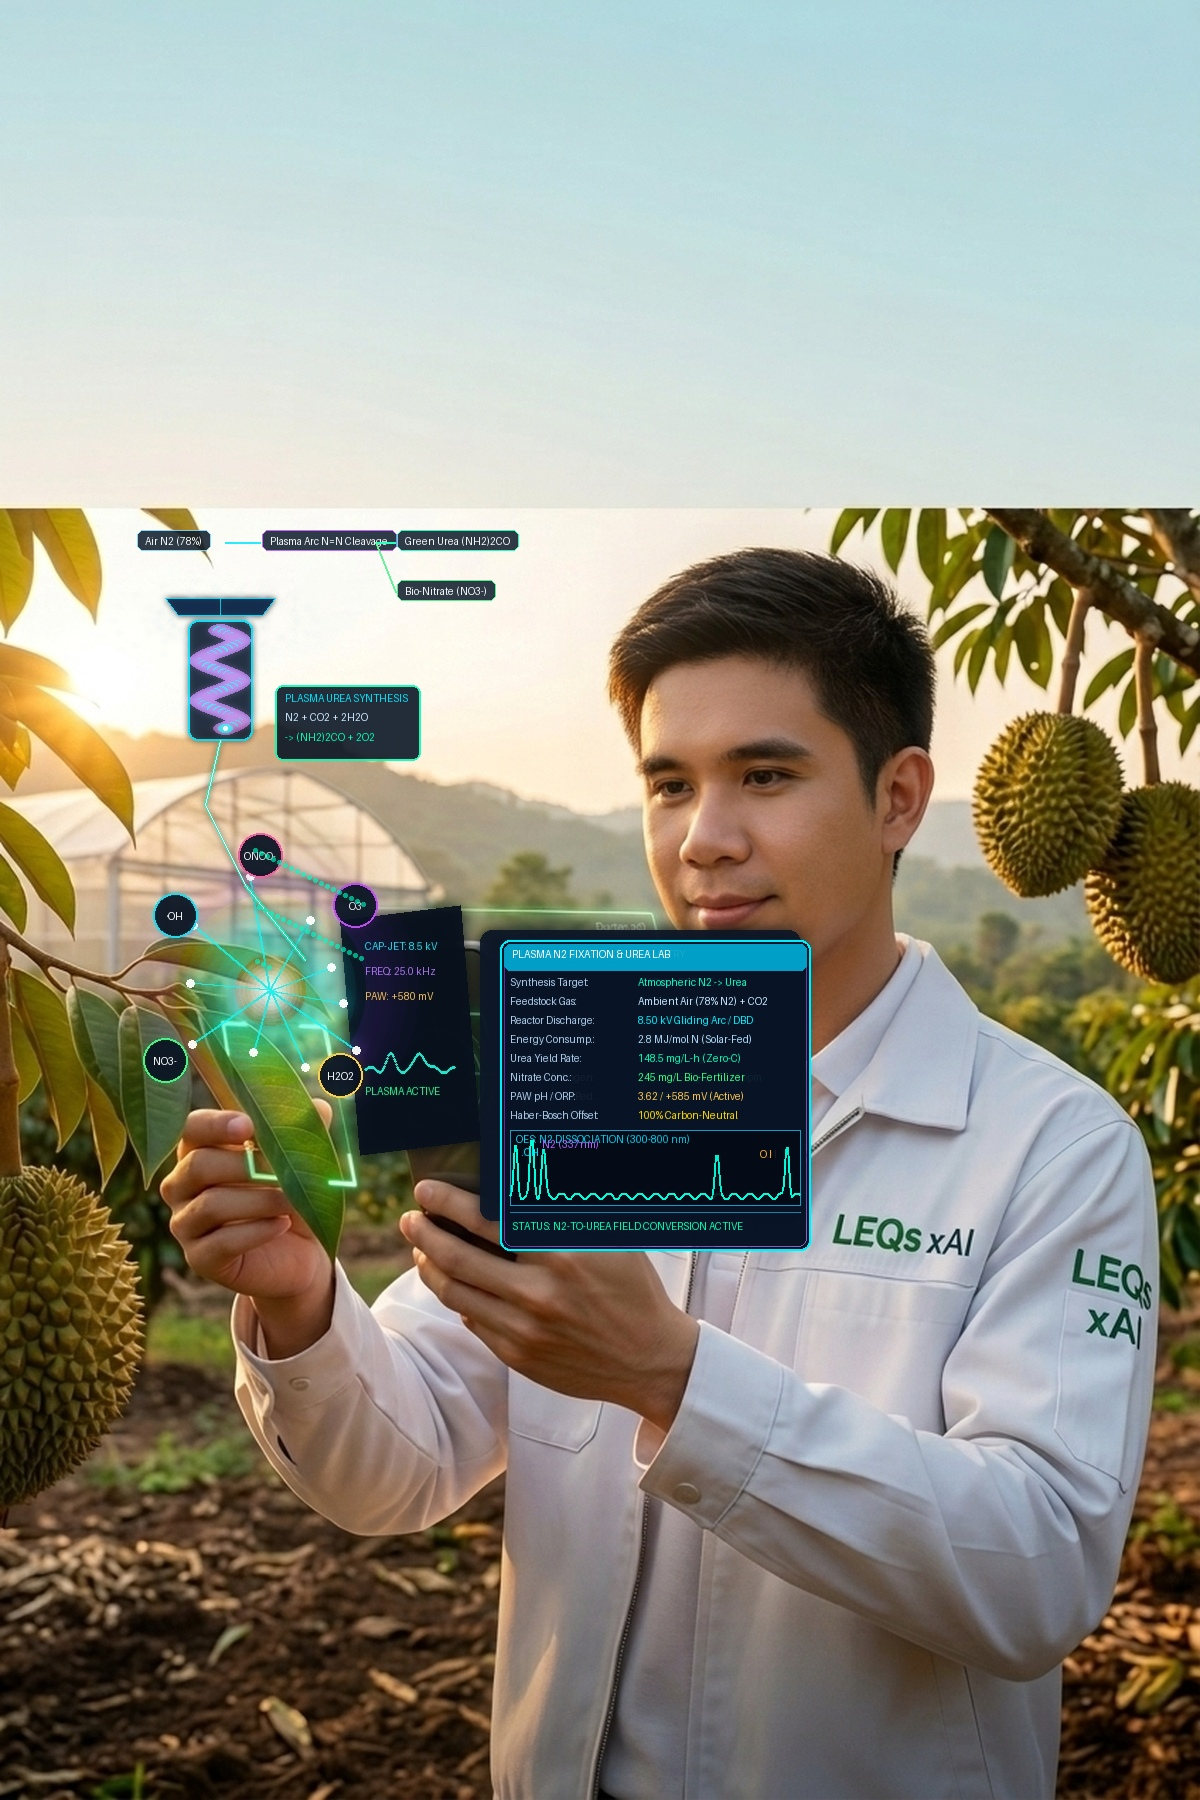
\includegraphics[width=\paperwidth,height=\paperheight]{figures/cover_art_concept_plasma_urea.jpg}
    };

    % 2. UPPER SKY ZONE: Transparent Architecture with Dual-Layer Micro Drop-Shadow
    % Shadow Layer (Soft white glow halo for crisp contrast against pastel morning sky)
    \node[anchor=north, align=center, text width=5.4in] at ([xshift=0.6pt, yshift=-0.076in]current page.north) {
        \begin{tikzpicture}
            \node[fill=deepIndigo!85, text=white, rounded corners=2.5mm, inner sep=3.5pt, font=\fontsize{7.5}{9.5}\selectfont\bfseries] {
                \color{cyberCyan}$\blacktriangleright$\ \color{white}TEXTBOOK SERIES IN APPLIED PHYSICS \& PLASMA AGRICULTURE\ \color{neonEmerald}$\blacktriangleleft$
            };
        \end{tikzpicture}\\[2.5pt]
        {\fontsize{8.5}{11}\selectfont\color{white}\textbf{ตำราวิชาการและคู่มือการวิจัยขั้นสูง \textbullet\ มหาวิทยาลัยราชภัฏรำไพพรรณี}}\\[3pt]
        
        % Main Title Line 1 (2.5x Size = 55pt in Pure White Shadow)
        {\fontsize{55}{62}\selectfont\bfseries\color{white} พลาสมาฟิสิกส์}\\[2pt]
        % Main Title Line 2
        {\fontsize{24}{30}\selectfont\bfseries\color{white} เพื่อการเกษตรและสิ่งแวดล้อม}\\[3.5pt]
        % Subtitle Pill Tag
        \begin{tikzpicture}
            \node[draw=cyberCyan, line width=1.1pt, rounded corners=2.5mm, inner sep=3.5pt] {
                \fontsize{11}{14}\selectfont\bfseries\color{white} จากทฤษฎีสู่นวัตกรรมความยั่งยืน
            };
        \end{tikzpicture}\\[3pt]
        % English Subtitle
        {\fontsize{8.2}{10.5}\selectfont\bfseries\color{white} PLASMA PHYSICS FOR AGRICULTURE AND ENVIRONMENT}\\[1.5pt]
        {\fontsize{7}{9}\selectfont\color{white} (FROM FUNDAMENTAL DISCHARGE PHYSICS TO SUSTAINABLE SMART AGRO-AI INNOVATION)}
    };

    % Foreground Layer (Crisp typography with Multicolored Plasma Spectrum)
    \node[anchor=north, align=center, text width=5.4in] at ([yshift=-0.08in]current page.north) {
        \begin{tikzpicture}
            \node[fill=deepIndigo!92, text=white, rounded corners=2.5mm, inner sep=3.5pt, font=\fontsize{7.5}{9.5}\selectfont\bfseries] {
                \color{cyberCyan}$\blacktriangleright$\ \color{white}TEXTBOOK SERIES IN APPLIED PHYSICS \& PLASMA AGRICULTURE\ \color{neonEmerald}$\blacktriangleleft$
            };
        \end{tikzpicture}\\[2.5pt]
        {\fontsize{8.5}{11}\selectfont\color{deepIndigo!90}\textbf{ตำราวิชาการและคู่มือการวิจัยขั้นสูง \textbullet\ มหาวิทยาลัยราชภัฏรำไพพรรณี}}\\[3pt]
        
        % Main Title Line 1 (2.5x Size = 55pt, Multicolored Plasma Spectrum)
        {\fontsize{55}{62}\selectfont\bfseries%
        {\color{specViolet}พลาส}%
        {\color{specCyan}มา}%
        {\color{specEmerald}ฟิ}%
        {\color{specCoral}สิกส์}%
        }\\[2pt]
        % Main Title Line 2
        {\fontsize{24}{30}\selectfont\bfseries\color{agriGreen!85!black} เพื่อการเกษตรและสิ่งแวดล้อม}\\[3.5pt]
        % Subtitle Pill Tag
        \begin{tikzpicture}
            \node[draw=cyberCyan!90, line width=1.1pt, fill=white!55, fill opacity=0.55, text opacity=1.0, rounded corners=2.5mm, inner sep=3.5pt] {
                \fontsize{11}{14}\selectfont\bfseries\color{deepIndigo} จากทฤษฎีสู่นวัตกรรมความยั่งยืน
            };
        \end{tikzpicture}\\[3pt]
        % English Subtitle
        {\fontsize{8.2}{10.5}\selectfont\bfseries\color{deepIndigo!95} PLASMA PHYSICS FOR AGRICULTURE AND ENVIRONMENT}\\[1.5pt]
        {\fontsize{7}{9}\selectfont\color{deepIndigo!80} (FROM FUNDAMENTAL DISCHARGE PHYSICS TO SUSTAINABLE SMART AGRO-AI INNOVATION)}
    };

    % 3. BOTTOM ZONE: Natural Dark Soil Canvas with Micro Shadow & Soft Depth Vignette
    \shade[top color=transparent, bottom color=black!85, opacity=0.90] 
        ([yshift=0.95in]current page.south west) rectangle (current page.south east);

    % Shadow Layer
    \node[anchor=south, align=center, text width=5.3in] at ([xshift=0.5pt, yshift=0.106in]current page.south) {
        {\fontsize{14}{18}\selectfont\bfseries\color{black!98} ผู้ช่วยศาสตราจารย์ ดร.ชีวะ ทัศนา}\\[2.5pt]
        {\fontsize{9}{12}\selectfont\bfseries\color{black!98} สาขาวิชาปัญญาประดิษฐ์เพื่อเกษตรดิจิทัลและสิ่งแวดล้อม คณะวิทยาศาสตร์และเทคโนโลยี}\\[2pt]
        {\fontsize{8.5}{11}\selectfont\bfseries\color{black!98} มหาวิทยาลัยราชภัฏรำไพพรรณี \textbullet\ พ.ศ. 2569}
    };
    % Foreground Layer
    \node[anchor=south, align=center, text width=5.3in] at ([yshift=0.11in]current page.south) {
        {\fontsize{14}{18}\selectfont\bfseries\color{white} ผู้ช่วยศาสตราจารย์ ดร.ชีวะ ทัศนา}\\[2.5pt]
        {\fontsize{9}{12}\selectfont\bfseries\color{white!98} สาขาวิชาปัญญาประดิษฐ์เพื่อเกษตรดิจิทัลและสิ่งแวดล้อม คณะวิทยาศาสตร์และเทคโนโลยี}\\[2pt]
        {\fontsize{8.5}{11}\selectfont\bfseries\color{techAmber} มหาวิทยาลัยราชภัฏรำไพพรรณี \textbullet\ พ.ศ. 2569}
    };
\end{tikzpicture}
\endgroup
\end{titlepage}
\cleardoublepage


% 2. Vector Inner Title Page (Dark-mode vector art with TikZ Bezier curves)
% =========================================================================
% Academic Book Cover Architect - Vector Inner Title Page (Dark Mode)
% 100% Vector Art with TikZ Bezier Curves & Zero-Artifact Typography
% =========================================================================

\thispagestyle{empty}
\begingroup
\setlength{\XeTeXlinebreakskip}{0pt}

\begin{tikzpicture}[remember picture, overlay]

% 1. Full-page Pure Dark Canvas
\fill[black!94] (current page.south west) rectangle (current page.north east);

% 2. Border frames in subtle gold and cyan
\draw[plasmaCyan!50, line width=0.8pt] 
    ([xshift=0.35in, yshift=-0.35in]current page.north west) rectangle 
    ([xshift=-0.35in, yshift=0.35in]current page.south east);

\draw[plasmaGold!55, line width=0.4pt] 
    ([xshift=0.38in, yshift=-0.38in]current page.north west) rectangle 
    ([xshift=-0.38in, yshift=0.38in]current page.south east);

% 3. Upper Typography
\node[anchor=north, align=center, text width=5.0in] 
      at ([yshift=-0.65in]current page.north) {
    {\fontsize{9}{12}\selectfont\color{plasmaCyan!90}\bfseries RAMBHAI BARNI RAJABHAT UNIVERSITY}\\[14pt]
    {\fontsize{18}{22}\selectfont\bfseries\color{white} พลาสมาฟิสิกส์และปัญญาประดิษฐ์}\\[4pt]
    {\fontsize{17}{21}\selectfont\bfseries\color{white} เพื่อการเกษตรและสิ่งแวดล้อม}\\[6pt]
    {\fontsize{11.5}{15}\selectfont\color{plasmaGold!95} จากฟิสิกส์การคายประจุและการเรียนรู้เชิงลึกสู่นวัตกรรมยั่งยืน}\\[8pt]
    {\fontsize{8.5}{11}\selectfont\bfseries\color{white!85} PLASMA PHYSICS AND ARTIFICIAL INTELLIGENCE FOR AGRICULTURE AND ENVIRONMENT\\(FROM DISCHARGE PHYSICS AND DEEP LEARNING TO SUSTAINABLE INNOVATIONS)}
};

% 4. Center 100% Vector Art: Agricultural Horizon & Cold Plasma Jet
\begin{scope}[shift={([yshift=-0.2in]current page.center)}]
    % Glowing Sun / Discharge Glow
    \shade[inner color=plasmaCyan!60!white, outer color=black!94, opacity=0.8]
        (0, 0.4in) circle (1.2in);
    
    % Mountain & Terrace Curves (Bezier)
    \draw[plasmaTeal!80, line width=1.0pt]
        (-2.2in, -0.4in) .. controls (-1.0in, 0.2in) and (0.6in, -0.3in) .. (2.2in, 0.1in);
    \draw[plasmaEmerald!75, line width=1.2pt]
        (-2.2in, -0.7in) .. controls (-0.8in, -0.4in) and (0.8in, -0.9in) .. (2.2in, -0.5in);
    \draw[plasmaLeaf!90, line width=1.5pt]
        (-2.2in, -1.0in) .. controls (-0.5in, -0.8in) and (0.5in, -1.2in) .. (2.2in, -0.9in);

    % Plasma Jet Column
    \draw[plasmaCyan!95, line width=2.5pt, opacity=0.9] (0, 0.9in) -- (0, -0.3in);
    \draw[white, line width=1.0pt] (0, 0.9in) -- (0, -0.3in);
    \fill[white] (0, 0.9in) circle (2.5pt);

    % Interaction Node with Sprout
    \draw[plasmaGold, line width=1.4pt] 
        (0, -0.3in) .. controls (0.2in, -0.1in) .. (0.35in, 0.05in);
    \fill[plasmaGold!95] (0.35in, 0.05in) ellipse (0.12in and 0.06in);
    \draw[plasmaCyan!90, line width=1.4pt] 
        (0, -0.3in) .. controls (-0.2in, -0.15in) .. (-0.30in, -0.05in);
    \fill[plasmaCyan!95] (-0.30in, -0.05in) ellipse (0.10in and 0.05in);

    % Constellation Network Nodes (IoT & AI monitoring)
    \foreach \pos in {(-1.5in, 0.6in), (-0.9in, 0.9in), (0.9in, 0.8in), (1.4in, 0.5in)} {
        \fill[plasmaCyan!90] \pos circle (2.2pt);
    }
    \draw[plasmaCyan!50, dashed, line width=0.6pt]
        (-1.5in, 0.6in) -- (-0.9in, 0.9in) -- (0, 0.9in) -- (0.9in, 0.8in) -- (1.4in, 0.5in);
\end{scope}

% 5. Lower Author Information (Crisp Vector Typography)
\node[anchor=south, align=center, text width=5.0in] 
      at ([yshift=0.65in]current page.south) {
    {\fontsize{13.5}{17}\selectfont\bfseries\color{white} ผู้ช่วยศาสตราจารย์ ดร.ชีวะ ทัศนา}\\[3pt]
    {\fontsize{9.5}{13}\selectfont\color{white!85} วท.บ. (ฟิสิกส์), วท.ม. (ฟิสิกส์), ปร.ด. (ฟิสิกส์)}\\[8pt]
    {\fontsize{9}{12}\selectfont\color{white!85} สาขาวิชาปัญญาประดิษฐ์เพื่อเกษตรดิจิทัลและสิ่งแวดล้อม คณะวิทยาศาสตร์และเทคโนโลยี}\\[3pt]
    {\fontsize{9}{12}\selectfont\color{plasmaCyan!95} มหาวิทยาลัยราชภัฏรำไพพรรณี}\\[6pt]
    {\fontsize{8.5}{11}\selectfont\color{plasmaGold!95} พ.ศ. 2569}
};

\end{tikzpicture}

\endgroup
\cleardoublepage


% 3. Preface (คำนำ)
\chapter*{คำนำ}
\addcontentsline{toc}{chapter}{คำนำ}

ในศตวรรษที่ 21 โลกกำลังเผชิญกับความท้าทายครั้งใหญ่ที่มีความเชื่อมโยงกันอย่างแยกไม่ออก นั่นคือการสร้างความมั่นคงทางอาหาร (Food Security) ควบคู่ไปกับการรักษาสมดุลทางนิเวศวิทยาและการฟื้นฟูสิ่งแวดล้อม (Environmental Sustainability) ภาคการเกษตรดั้งเดิมที่พึ่งพาปุ๋ยเคมีสังเคราะห์ ยาปราบศัตรูพืช และพลังงานฟอสซิลอย่างเข้มข้น ไม่เพียงแต่ส่งผลให้เกิดการเสื่อมโทรมของทรัพยากรดินและน้ำ หากยังเป็นแหล่งปลดปล่อยก๊าซเรือนกระจกที่สำคัญ ยิ่งไปกว่านั้น ปัญหามลพิษทางอากาศ ขยะอุตสาหกรรม และการปนเปื้อนของสารเคมีอันตรายที่ย่อยสลายยากในสิ่งแวดล้อม ได้ทวีความรุนแรงจนส่งผลกระทบต่อสุขภาพของมนุษย์และสิ่งมีชีวิตในระบบนิเวศอย่างไม่อาจหลีกเลี่ยงได้

ท่ามกลางวิกฤตการณ์เหล่านี้ การบูรณาการองค์ความรู้ข้ามศาสตร์ (Interdisciplinary Integration) ได้กลายเป็นกุญแจสำคัญในการแสวงหาทางออกใหม่ที่ยั่งยืน \textbf{เทคโนโลยีพลาสมา (Plasma Technology)} ซึ่งเดิมทีเป็นศาสตร์ทางฟิสิกส์ขั้นสูงที่ถูกจำกัดอยู่ในวงการดาราศาสตร์ พลังงานนิวเคลียร์ฟิวชัน อุตสาหกรรมเซมิคอนดักเตอร์ และวิศวกรรมวัสดุศาสตร์ ได้ก้าวข้ามขีดจำกัดเดิมผ่านการพัฒนาเทคโนโลยีพลาสมาความดันบรรยากาศอุณหภูมิต่ำ หรือพลาสมาเย็น (Cold Atmospheric Plasma หรือ CAP) ที่สามารถทำงานได้ในสภาวะแวดล้อมปกติโดยไม่ต้องใช้ระบบสุญญากาศที่ซับซ้อนและสิ้นเปลืองพลังงาน

ความก้าวหน้าดังกล่าวได้เปิดพรมแดนใหม่ที่เรียกว่า \textbf{พลาสมาเพื่อการเกษตร (Plasma Agriculture)} และ \textbf{พลาสมาเพื่อการจัดการสิ่งแวดล้อม (Environmental Plasma Technology)} โดยอาศัยกลไกอันเป็นเอกลักษณ์ของพลาสมาในการผลิตอนุภาคที่มีความว่องไวทางเคมีสูง โดยเฉพาะอนุมูลอิสระของออกซิเจนและไนโตรเจน (Reactive Oxygen and Nitrogen Species หรือ RONS) สนามแม่เหล็กไฟฟ้า และรังสียูวี โดยใช้เพียงอากาศ น้ำ และพลังงานไฟฟ้าเป็นวัตถุดิบตั้งต้น เทคโนโลยีนี้จึงเปรียบเสมือนโรงงานเคมีสีเขียวขนาดจิ๋วที่สามารถกระตุ้นความงอกของเมล็ดพันธุ์ ตรึงไนโตรเจนจากอากาศมาสร้างเป็นปุ๋ยน้ำ (Plasma-Activated Water หรือ PAW) ยับยั้งเชื้อก่อโรคพืชและจุลินทรีย์ปนเปื้อนในอาหารหลังการเก็บเกี่ยว ตลอดจนย่อยสลายสารพิษตกค้างและมลพิษในน้ำ ดิน และอากาศได้อย่างมีประสิทธิภาพโดยไม่ทิ้งสารเคมีตกค้าง

หนังสือ \textbf{พลาสมาฟิสิกส์และปัญญาประดิษฐ์ เพื่อการเกษตรและสิ่งแวดล้อม: จากฟิสิกส์การคายประจุและการเรียนรู้เชิงลึกสู่นวัตกรรมยั่งยืน} เล่มนี้ เรียบเรียงขึ้นโดยมีวัตถุประสงค์เพื่อเป็นสะพานเชื่อมองค์ความรู้ระหว่างนักฟิสิกส์ วิศวกร นักวิทยาศาสตร์การเกษตร นักจุลชีววิทยา และนักวิทยาศาสตร์สิ่งแวดล้อม เนื้อหาภายในเล่มได้รับการออกแบบให้มีความต่อเนื่องอย่างเป็นระบบ เริ่มตั้งแต่การปูพื้นฐานทางฟิสิกส์ของสถานะพลาสมาและเคมีของการคายประจุในก๊าซด้วยภาษาที่เข้าใจง่าย ไปจนถึงการเจาะลึกกลไกระดับเซลล์และโมเลกุลในการประยุกต์ใช้งานทางการเกษตรตั้งแต่ต้นน้ำถึงปลายน้ำ การบำบัดมลพิษสิ่งแวดล้อมครบวงจร และการออกแบบขยายขนาดระบบสู่การใช้งานจริงในระดับอุตสาหกรรม

ผู้เขียนหวังเป็นอย่างยิ่งว่า หนังสือเล่มนี้จะเป็นประโยชน์ต่อนักศึกษาระดับปริญญาตรีและบัณฑิตศึกษา คณาจารย์ นักวิจัย ตลอดจนผู้ประกอบการด้านเทคโนโลยีเกษตรสมัยใหม่ (AgriTech) และเทคโนโลยีสะอาด (CleanTech) ในการใช้เป็นตำราเรียน เอกสารอ้างอิง และแรงบันดาลใจในการสร้างสรรค์งานวิจัยและนวัตกรรมพลาสมา เพื่อร่วมกันขับเคลื่อนภาคการเกษตรและการจัดการสิ่งแวดล้อมของประเทศไทยให้ก้าวสู่ความยั่งยืนอย่างแท้จริง

\vspace{1.5cm}
\begin{flushright}
    \textbf{ผู้ช่วยศาสตราจารย์ ดร.ชีวะ ทัศนา}\\
    สาขาวิชาปัญญาประดิษฐ์เพื่อเกษตรดิจิทัลและสิ่งแวดล้อม\\
    คณะวิทยาศาสตร์และเทคโนโลยี มหาวิทยาลัยราชภัฏรำไพพรรณี\\
    พ.ศ. 2569
\end{flushright}

\clearpage


% 4. Table of Contents & Lists
\tableofcontents
\clearpage
\listoffigures
\clearpage
\listoftables
\cleardoublepage

% -------------------------------------------------------------------------
% Main Matter (Chapters)
% -------------------------------------------------------------------------
\mainmatter

% Part 1: พื้นฐานพลาสมาฟิสิกส์ เคมีพลาสมา และการวินิจฉัย
\part{พื้นฐานพลาสมาฟิสิกส์ เคมีพลาสมา และการวินิจฉัย}
\chapter{บทนำสู่สถานะที่สี่ของสสาร}
\label{chap:ch01}

% =========================================================================
% แผนบริหารการสอนประจำบทที่ 1 (Modular Lesson Plan Boxes - 2-Page Standard)
% =========================================================================

\section*{แผนบริหารการสอนประจำบทที่ 1}
\addcontentsline{toc}{section}{แผนบริหารการสอนประจำบทที่ 1}

% --- Page 1 of Lesson Plan ---
\begin{planbox}{หัวข้อเนื้อหาประจำบท}
\begin{enumerate}
    \item สถานะที่สี่ของสสารและการเปลี่ยนสถานะจากของแข็งสู่พลาสมา
    \item องค์ประกอบของพลาสมาและกลุ่มอนุภาคว่องไวทางเคมี
    \item นิยามและคุณสมบัติพื้นฐานทางฟิสิกส์ของพลาสมา
    \item การจำแนกประเภทพลาสมาตามสมดุลทางอุณหพลศาสตร์
    \item บทบาทและความสำคัญของพลาสมาในงานเกษตรกรรมและสิ่งแวดล้อม
\end{enumerate}
\end{planbox}

\begin{planbox}{วัตถุประสงค์เชิงพฤติกรรม}
\begin{enumerate}
    \item อธิบายกลไกการเปลี่ยนสถานะของสสารจนเกิดเป็นสถานะพลาสมาได้อย่างถูกต้อง
    \item ระบุองค์ประกอบสำคัญ 6 ชนิดภายในพลาสมาความดันบรรยากาศได้อย่างครบถ้วน
    \item คำนวณค่าความยาวเดอบาย ระดับการแตกตัวเป็นไอออน และแปลงหน่วยพลังงานอิเล็กตรอนโวลต์ได้อย่างถูกต้อง
    \item จำแนกความแตกต่างระหว่างพลาสมาสมดุลความร้อนและพลาสมาไม่สมดุลความร้อนได้อย่างชัดเจน
    \item วิเคราะห์ข้อได้เปรียบของการประยุกต์ใช้พลาสมาเย็นในงานเกษตรและสิ่งแวดล้อมได้อย่างเป็นระบบ
\end{enumerate}
\end{planbox}

\newpage

% --- Page 2 of Lesson Plan ---
\begin{planbox}{วิธีสอนและกิจกรรมการเรียนการสอน}
\begin{enumerate}
    \item บรรยายเชิงปฏิสัมพันธ์ประกอบสื่อมัลติมีเดียและแบบจำลองทฤษฎีการกำบังเดอบาย
    \item อภิปรายกลุ่มย่อยเกี่ยวกับการเปรียบเทียบข้อดีและข้อจำกัดของพลาสมาอุณหภูมิห้อง
    \item สาธิตการสร้างพลาสมาเจ็ทและการคายประจุแบบกั้นด้วยไดอิเล็กทริกจำลอง
    \item ศึกษาค้นคว้ากรณีศึกษาการใช้น้ำกระตุ้นด้วยพลาสมาเพื่อทดแทนปุ๋ยเคมีไนโตรเจน
    \item สรุปบทเรียนร่วมกันและทำแบบฝึกหัดทบทวนท้ายบท
\end{enumerate}
\end{planbox}

\begin{planbox}{สื่อการเรียนการสอน}
\begin{enumerate}
    \item เอกสารประกอบการสอนและตำราวิชาการ พลาสมาฟิสิกส์เพื่อการเกษตรและสิ่งแวดล้อม
    \item สไลด์การสอนอิเล็กทรอนิกส์และภาพประกอบเวกเตอร์ความละเอียดสูง
    \item วิดีโอทัศน์การทดลองการคายประจุพลาสมาความดันบรรยากาศและการวัดสเปกตรัมแสง
    \item ชุดคำถามทบทวนประจำบทและใบกิจกรรมวิเคราะห์บทความวิจัยสากล
\end{enumerate}
\end{planbox}

\begin{planbox}{การวัดและประเมินผล}
\begin{enumerate}
    \item ประเมินจากการมีส่วนร่วมในการอภิปรายและตอบคำถามในชั้นเรียน ร้อยละ 10
    \item ประเมินจากความถูกต้องในการทำแบบฝึกหัดทบทวนท้ายบท ร้อยละ 10
    \item ประเมินจากรายงานการวิเคราะห์กรณีศึกษาเทคโนโลยีพลาสมา ร้อยละ 10
    \item ประเมินจากการสอบวัดผลสัมฤทธิ์ประจำภาคการศึกษา ร้อยละ 70
\end{enumerate}
\end{planbox}

\clearpage

% =========================================================================
% เนื้อหาบทเรียน (เริ่มต้นหน้า 3 อย่างเป็นระเบียบ)
% =========================================================================

\section{สถานะที่สี่ของสสารและการเปลี่ยนสถานะ}

สสารในธรรมชาติที่เราคุ้นเคยในชีวิตประจำวันประกอบด้วยสามสถานะหลัก ได้แก่ ของแข็ง (Solid) ของเหลว (Liquid) และก๊าซ (Gas) หากเราพิจารณาน้ำแข็งซึ่งเป็นของแข็ง เมื่อได้รับพลังงานความร้อน พันธะระหว่างโมเลกุลจะอ่อนกำลังลงจนหลอมเหลวกลายเป็นน้ำในสถานะของเหลว และเมื่อให้พลังงานความร้อนต่อไปจนถึงจุดเดือด โมเลกุลของน้ำจะเคลื่อนที่ด้วยความเร็วสูงขึ้นจนหลุดออกจากกันและกลายเป็นไอน้ำในสถานะก๊าซ

คำถามสำคัญทางฟิสิกส์คือ หากเรายังคงป้อนพลังงานความร้อนหรือพลังงานไฟฟ้าเข้าไปยังก๊าซอย่างต่อเนื่องที่อุณหภูมิสูงขึ้นอย่างมหาศาลจะเกิดอะไรขึ้น พลังงานจลน์ที่สูงขึ้นจะทำให้อนุภาคในก๊าซชนกันอย่างรุนแรงจนทำให้อิเล็กตรอนวงนอกสุดหลุดออกจากอะตอมหรือโมเลกุล กระบวนการนี้เรียกว่า \textbf{การแตกตัวเป็นไอออน (Ionization)} ส่งผลให้กลุ่มก๊าซเดิมแปรสภาพกลายเป็นกลุ่มหมอกของอนุภาคที่มีประจุไฟฟ้า ประกอบด้วยอิเล็กตรอนอิสระ ไอออนบวก อะตอมหรือโมเลกุลที่ยังไม่แตกตัว ตลอดจนอนุมูลอิสระและรังสีแม่เหล็กไฟฟ้า สภาวะใหม่นี้เรียกว่า \textbf{พลาสมา (Plasma)} ซึ่งได้รับการยอมรับว่าเป็น \textbf{สถานะที่สี่ของสสาร (Fourth State of Matter)}

\begin{figure}[H]
\centering
\begin{tikzpicture}[scale=0.68, every node/.style={transform shape}]
    % Four states boxes
    \draw[rounded corners=6pt, fill=blue!10, draw=blue!60, line width=1pt] (-5.5, 0) rectangle (-3.0, 3.2);
    \node at (-4.25, 2.8) {\bfseries ของแข็ง};
    \node at (-4.25, 2.4) {\small (Solid)};
    \foreach \x in {-5.0, -4.5, -4.0, -3.5} {
        \foreach \y in {0.5, 1.0, 1.5, 2.0} {
            \fill[blue!70!black] (\x, \y) circle (3pt);
        }
    }

    \draw[->, >=Stealth, line width=1.5pt, red!70] (-2.8, 1.6) -- (-2.0, 1.6);
    \node[above, red!70] at (-2.4, 1.6) {\scriptsize +ความร้อน};

    \draw[rounded corners=6pt, fill=cyan!10, draw=cyan!60, line width=1pt] (-1.8, 0) rectangle (0.7, 3.2);
    \node at (-0.55, 2.8) {\bfseries ของเหลว};
    \node at (-0.55, 2.4) {\small (Liquid)};
    \foreach \pos in {(-1.4, 0.4), (-1.0, 0.7), (-0.5, 0.5), (0.2, 0.6), (-1.2, 1.2), (-0.7, 1.5), (0.1, 1.3), (-0.9, 2.0), (-0.2, 1.9)} {
        \fill[cyan!70!black] \pos circle (3.2pt);
    }

    \draw[->, >=Stealth, line width=1.5pt, red!70] (0.9, 1.6) -- (1.7, 1.6);
    \node[above, red!70] at (1.3, 1.6) {\scriptsize +ความร้อน};

    \draw[rounded corners=6pt, fill=yellow!10, draw=yellow!60!black, line width=1pt] (1.9, 0) rectangle (4.4, 3.2);
    \node at (3.15, 2.8) {\bfseries ก๊าซ};
    \node at (3.15, 2.4) {\small (Gas)};
    \foreach \pos in {(2.4, 0.8), (3.8, 0.6), (3.1, 1.4), (2.5, 2.1), (3.9, 1.9)} {
        \fill[yellow!60!black] \pos circle (3.5pt);
    }

    \draw[->, >=Stealth, line width=1.5pt, plasmaViolet] (4.6, 1.6) -- (5.4, 1.6);
    \node[above, plasmaViolet] at (5.0, 1.6) {\scriptsize +พลังงานไฟฟ้า};

    \draw[rounded corners=6pt, fill=plasmaViolet!10, draw=plasmaViolet, line width=1.2pt] (5.6, 0) rectangle (8.3, 3.2);
    \node at (6.95, 2.8) {\bfseries พลาสมา};
    \node at (6.95, 2.4) {\small (Plasma)};
    % Ions and electrons
    \foreach \pos in {(6.1, 0.8), (7.7, 0.7), (6.9, 1.5), (6.3, 2.1), (7.6, 2.0)} {
        \fill[red!70!black] \pos circle (4pt);
        \node[white] at \pos {\tiny +};
    }
    \foreach \pos in {(6.4, 0.5), (7.2, 0.9), (6.5, 1.2), (7.4, 1.6), (6.8, 2.2), (7.9, 2.4)} {
        \fill[blue!80!white] \pos circle (2pt);
        \node[white] at \pos {\scalebox{0.5}{$-$}};
    }
\end{tikzpicture}
\caption{การเปลี่ยนสถานะของสสารจากของแข็ง ของเหลว ก๊าซ สู่สถานะพลาสมาผ่านการแตกตัวเป็นไอออน}
\label{fig:four_states}
\end{figure}

แม้ว่าบนผิวโลกสสารส่วนใหญ่จะอยู่ในสถานะของแข็ง ของเหลว หรือก๊าซ แต่ในเอกภพโดยรวม สสารมากกว่าร้อยละ 99 อยู่ในสถานะพลาสมา เช่น ดวงอาทิตย์ ดวงดาวในกาแล็กซี เนบิวลา และสสารระหว่างดวงดาว บนผิวโลกเราสามารถพบพลาสมาตามธรรมชาติได้ในปรากฏการณ์ฟ้าผ่า (Lightning) และแสงเหนือแสงใต้ (Aurora)

\subsection{องค์ประกอบของพลาสมาความดันบรรยากาศ}

เมื่อก๊าซเปลี่ยนสถานะเป็นพลาสมา โดยเฉพาะพลาสมาที่เกิดจากการคายประจุในอากาศหรือก๊าซผสมที่ความดันบรรยากาศ ภายในพลาสมาจะมีกลุ่มอนุภาคและองค์ประกอบสำคัญ 6 ชนิด ได้แก่

\begin{enumerate}
    \item \textbf{อิเล็กตรอนอิสระ (Free Electrons หรือ $e^-$)} มีมวลน้อยมาก เคลื่อนที่ได้รวดเร็ว และเป็นตัวรับพลังงานหลักจากสนามไฟฟ้าภายนอกเพื่อถ่ายทอดพลังงานให้แก่อนุภาคอื่นๆ
    \item \textbf{ไอออนบวกและไอออนลบ (Positive and Negative Ions)} เกิดจากการที่อะตอมหรือโมเลกุลสูญเสียอิเล็กตรอน เช่น \ce{N2+}, \ce{O2+}, \ce{Ar+} หรือรับอิเล็กตรอนเพิ่ม เช่น \ce{O2-}, \ce{O-}
    \item \textbf{อะตอมและโมเลกุลในสถานะกระตุ้น (Excited Species and Metastables)} อนุภาคที่ได้รับพลังงานจากการชนแต่อิเล็กตรอนยังไม่หลุดออก เช่น \ce{O(^1D)}, \ce{N2(A^3{$\Sigma$}_u^+)} ซึ่งมีอายุขัยยาวนานและมีบทบาทสำคัญในการถ่ายโอนพลังงานเคมี
    \item \textbf{อนุมูลอิสระและสารว่องไวทางเคมี (Reactive Species หรือ RONS)} เกิดจากการแตกพันธะเคมีของก๊าซและไอน้ำในบรรยากาศ เช่น อนุมูลไฮดรอกซิล ($\cdot\ce{OH}$), โอโซน (\ce{O3}), ไฮโดรเจนเปอร์ออกไซด์ (\ce{H2O2}), ไนตริกออกไซด์ ($\cdot\ce{NO}$)
    \item \textbf{โฟตอนและรังสีแม่เหล็กไฟฟ้า (Photons and UV Radiation)} แสงที่ปลดปล่อยออกมาจากการเปลี่ยนระดับพลังงานของอิเล็กตรอน มีตั้งแต่แสงที่ตามองเห็นไปจนถึงรังสีอัลตราไวโอเลตสุญญากาศ (VUV)
    \item \textbf{สนามไฟฟ้าเฉพาะที่และคลื่นกระแทก (Local Electric Fields and Micro-shockwaves)} สนามไฟฟ้าความเข้มสูงระดับไมโครสเกลที่เกิดขึ้นระหว่างการเคลื่อนที่ของกลุ่มประจุ
\end{enumerate}

\section{นิยามและคุณสมบัติพื้นฐานทางฟิสิกส์ของพลาสมา}

ในทางฟิสิกส์ ก๊าซที่แตกตัวเป็นไอออนจะถือว่าเป็นพลาสมาได้อย่างแท้จริงก็ต่อเมื่อมีคุณสมบัติทางกายภาพครบ 3 ประการ ได้แก่ ความเป็นกลางทางไฟฟ้าโดยรวม การกำบังเดอบาย และพฤติกรรมรวมหมู่

\subsection{ความเป็นกลางทางไฟฟ้าโดยรวม}

แม้ว่าพลาสมาจะประกอบด้วยอนุภาคที่มีประจุไฟฟ้าลบและบวกจำนวนมหาศาล แต่เมื่อพิจารณาในปริมาตรมหภาค (Macroscopic scale) ประจุบวกและประจุลบจะหักล้างกันจนมีค่าสุทธิเป็นศูนย์ ความสัมพันธ์นี้เขียนได้ในรูป
\begin{equation}
    n_e \approx \sum_i Z_i n_i = n
\end{equation}
โดยที่ $n_e$ คือความหนาแน่นของอิเล็กตรอน ($m^{-3}$), $n_i$ คือความหนาแน่นของไอออนที่มีประจุ $Z_i$, และ $n$ เรียกว่าความหนาแน่นพลาสมา (Plasma Density)

\subsection{การกำบังเดอบายและความยาวเดอบาย}

เมื่อมีประจุไฟฟ้าแปลกปลอมหรือขั้วไฟฟ้าใส่เข้าไปในพลาสมา อนุภาคประจุตรงข้ามจะเคลื่อนที่เข้ามาล้อมรอบเพื่อบดบังสนามไฟฟ้าของประจุนั้น ปรากฏการณ์นี้เรียกว่า \textbf{การกำบังเดอบาย (Debye Shielding)} ระยะทางที่สนามไฟฟ้าลดลงเหลือ $1/e$ หรือประมาณร้อยละ 37 ของค่าเดิม เรียกว่า \textbf{ความยาวเดอบาย (Debye Length, $\lambda_D$)} ซึ่งมีนิยามตามสมการ
\begin{equation}
    \lambda_D = \sqrt{\frac{\varepsilon_0 k_B T_e}{n_e e^2}}
    \label{eq:debye_length}
\end{equation}
โดยที่ $\varepsilon_0 = 8.854 \times 10^{-12}\text{ F/m}$ คือสภาพยอมทางไฟฟ้าในสุญญากาศ, $k_B = 1.381 \times 10^{-23}\text{ J/K}$ คือค่าคงที่โบลต์ซมันน์, $T_e$ คืออุณหภูมิของอิเล็กตรอน (K), $n_e$ คือความหนาแน่นของอิเล็กตรอน ($m^{-3}$), และ $e = 1.602 \times 10^{-19}\text{ C}$ คือประจุของอิเล็กตรอน

\begin{figure}[H]
\centering
\begin{tikzpicture}[scale=0.95]
    % Central positive test charge
    \shade[inner color=red!80!white, outer color=red!90!black] (0,0) circle (0.35cm);
    \node[white, font=\bfseries] at (0,0) {$+Q$};

    % Debye sphere boundary
    \draw[dashed, line width=1.2pt, plasmaViolet!80] (0,0) circle (2.2cm);
    \draw[<->, >=Stealth, line width=1pt, plasmaNavy] (0,0) -- (1.55, 1.55);
    \node[above left, font=\small\bfseries, plasmaNavy] at (0.85, 0.85) {$\lambda_D$};

    % Surrounding electrons inside Debye sphere
    \foreach \angle in {25, 65, 110, 150, 195, 235, 280, 320, 350} {
        \fill[blue!70!white] (\angle:1.1cm) circle (2.5pt);
        \node[white] at (\angle:1.1cm) {\scalebox{0.5}{$-$}};
    }
    \foreach \angle in {15, 45, 85, 130, 175, 215, 260, 305, 340} {
        \fill[blue!70!white] (\angle:1.8cm) circle (2.5pt);
        \node[white] at (\angle:1.8cm) {\scalebox{0.5}{$-$}};
    }

    % Outer undisturbed quasi-neutral plasma
    \node[right, font=\small, plasmaNavy] at (2.4, 1.2) {บริเวณพลาสมาปกติ};
    \node[right, font=\footnotesize, gray!80!black] at (2.4, 0.7) {สนามไฟฟ้าภายนอกถูกบดบัง};
    \node[right, font=\footnotesize, plasmaViolet] at (2.4, -0.3) {ขอบเขตทรงกลมเดอบาย ($\lambda_D$)};
\end{tikzpicture}
\caption{การจัดเรียงกลุ่มหมอกอิเล็กตรอนล้อมรอบประจุทดสอบตามหลักการกำบังเดอบาย}
\label{fig:debye_shielding}
\end{figure}

ระบบก๊าซที่แตกตัวเป็นไอออนจะมีพฤติกรรมเป็นพลาสมาได้ต่อเมื่อขนาดทางกายภาพของระบบ ($L$) มีค่ามากกว่าความยาวเดอบายอย่างมีนัยสำคัญ นั่นคือ $L \gg \lambda_D$

\subsection{พฤติกรรมรวมหมู่และความถี่พลาสมา}

เนื่องจากแรงระหว่างอนุภาคที่มีประจุเป็นแรงคูลอมบ์ระยะไกล (Long-range Coulomb Force) การเคลื่อนที่ของอนุภาคหนึ่งจึงส่งผลต่ออนุภาคอื่นๆ พร้อมกัน เกิดเป็น \textbf{พฤติกรรมรวมหมู่ (Collective Behavior)} หากกลุ่มอิเล็กตรอนถูกรบกวนให้เคลื่อนที่ออกจากตำแหน่งสมดุล แรงดึงดูดทางไฟฟ้าจะดึงกลับเข้ามา เกิดการกวัดแกว่งรอบตำแหน่งสมดุลด้วย \textbf{ความถี่พลาสมาของอิเล็กตรอน (Electron Plasma Frequency, $\omega_{pe}$)}
\begin{equation}
    \omega_{pe} = \sqrt{\frac{n_e e^2}{\varepsilon_0 m_e}}
\end{equation}
โดยที่ $m_e = 9.109 \times 10^{-31}\text{ kg}$ คือมวลของอิเล็กตรอน

\subsection{ระดับการแตกตัวเป็นไอออนและอุณหภูมิในพลาสมา}

ระดับการแตกตัวเป็นไอออน ($\alpha$) นิยามเป็นสัดส่วนของความหนาแน่นไอออนเทียบกับอนุภาคทั้งหมด
\begin{equation}
    \alpha = \frac{n_i}{n_i + n_n}
\end{equation}
โดยที่ $n_n$ คือความหนาแน่นของอนุภาคที่เป็นกลาง ในพลาสมาความดันบรรยากาศอุณหภูมิต่ำ ค่า $\alpha$ มีค่าอยู่ในช่วง $10^{-7}$ ถึง $10^{-4}$ ซึ่งหมายความว่าโมเลกุลของอากาศส่วนใหญ่ยังคงเป็นก๊าซปกติ ทำให้อุณหภูมิรวมของก๊าซยังคงใกล้เคียงอุณหภูมิห้อง

ในทางฟิสิกส์พลาสมา นิยมวัดอุณหภูมิของอนุภาคในหน่วย \textbf{อิเล็กตรอนโวลต์ (Electron-Volt หรือ eV)} โดยแปลงเป็นเคลวินได้ตามความสัมพันธ์
\begin{equation}
    1\text{ eV} = \frac{e}{k_B} \approx 11,600\text{ K}
\end{equation}

\begin{focusbox}{ความสำคัญทางฟิสิกส์ของหน่วยอิเล็กตรอนโวลต์}
เมื่อกล่าวว่าพลาสมาเย็นมีอุณหภูมิอิเล็กตรอน $T_e = 2\text{ eV}$ หมายความว่าเฉพาะตัวอิเล็กตรอนมีพลังงานจลน์เฉลี่ยเทียบเท่าอุณหภูมิ $23,200\text{ K}$ ซึ่งมีพลังงานเพียงพอที่จะชนและตัดพันธะเคมีของก๊าซเพื่อสร้างอนุมูลอิสระ RONS ได้อย่างมหาศาล แต่เนื่องจากอิเล็กตรอนมีมวลน้อยมากและก๊าซส่วนใหญ่ไม่แตกตัว อุณหภูมิรวมที่เรารู้สึกเมื่อสัมผัสจึงยังคงอยู่ที่ $25 - 40^\circ\text{C}$
\end{focusbox}

\section{การจำแนกประเภทพลาสมาตามสมดุลทางอุณหพลศาสตร์}

การจำแนกพลาสมาตามความสัมพันธ์ระหว่างอุณหภูมิของอิเล็กตรอน ($T_e$), อุณหภูมิของไอออน ($T_i$), และอุณหภูมิของก๊าซ ($T_g$) แบ่งออกเป็น 2 ประเภทหลัก

\subsection{พลาสมาสมดุลความร้อน}

พลาสมาสมดุลความร้อน (Thermal Plasma) หรือพลาสมาร้อน เป็นสภาวะที่อนุภาคทุกชนิดมีพลังงานจลน์เฉลี่ยเท่ากันในระดับสมดุลอุณหพลศาสตร์เฉพาะที่ (Local Thermodynamic Equilibrium หรือ LTE)
\begin{equation}
    T_e \approx T_i \approx T_g \quad (5,000 - 50,000\text{ K})
\end{equation}
มีลักษณะเด่นคือให้พลังงานความร้อนสูงมหาศาล ความหนาแน่นอิเล็กตรอนสูง ($10^{21} - 10^{26}\text{ m}^{-3}$) เหมาะสำหรับงานเผาทำลายขยะติดเชื้อ การหลอมกากพิษให้กลายเป็นแก้วเสถียร (Vitrification) และการแก๊สซิฟิเคชันเพื่อเปลี่ยนชีวมวลเป็นพลังงาน

\subsection{พลาสมาไม่สมดุลความร้อนหรือพลาสมาเย็น}

พลาสมาไม่สมดุลความร้อน (Non-thermal Plasma) หรือพลาสมาเย็นความดันบรรยากาศ (Cold Atmospheric Plasma หรือ CAP) เป็นสภาวะที่พลังงานไฟฟ้าถูกถ่ายทอดให้แก่อิเล็กตรอนเป็นหลัก โดยที่ไอออนและโมเลกุลก๊าซยังคงมีพลังงานจลน์ต่ำ
\begin{equation}
    T_e \gg T_i \approx T_g \quad (T_e \approx 10,000 - 100,000\text{ K}, \text{ แต่ } T_g \approx 300 - 320\text{ K})
\end{equation}
ลักษณะเด่นคือไม่ทำลายเนื้อเยื่อพืชหรือวัสดุทางชีววิทยาที่บอบบาง แต่สามารถกระตุ้นปฏิกิริยาเคมีขั้นสูงได้ที่อุณหภูมิห้อง

\begin{table}[H]
\caption{การเปรียบเทียบคุณสมบัติระหว่างพลาสมาสมดุลความร้อนและพลาสมาไม่สมดุลความร้อน}
\label{tab:plasma_comparison}
\begin{tabularx}{\textwidth}{p{3.2cm}X X}
\toprule
\textbf{พารามิเตอร์} & \textbf{พลาสมาสมดุลความร้อน} & \textbf{พลาสมาเย็น (CAP)} \\
\midrule
สถานะอุณหพลศาสตร์ & สมดุลเฉพาะที่ ($T_e \approx T_i \approx T_g$) & ไม่สมดุล ($T_e \gg T_i \approx T_g$) \\
อุณหภูมิอิเล็กตรอน ($T_e$) & $1 - 5\text{ eV}$ ($10,000 - 50,000\text{ K}$) & $1 - 10\text{ eV}$ ($10,000 - 100,000\text{ K}$) \\
อุณหภูมิก๊าซรวม ($T_g$) & $5,000 - 50,000\text{ K}$ & $300 - 320\text{ K}$ ($25 - 45^\circ\text{C}$) \\
ความหนาแน่นอิเล็กตรอน & $10^{21} - 10^{26}\text{ m}^{-3}$ & $10^{14} - 10^{20}\text{ m}^{-3}$ \\
ระดับการแตกตัว ($\alpha$) & สูง ($10^{-1}$ ถึง $100\%$) & ต่ำมาก ($10^{-7}$ ถึง $10^{-4}$) \\
กลไกการทำงานหลัก & กระบวนการความร้อนสูง (Pyrolysis) & เคมีพลาสมาจากอนุภาค RONS \\
การประยุกต์ใช้ & กำจัดขยะอันตราย, หลอมกากโลหะ & กระตุ้นเมล็ด, ปุ๋ยน้ำ PAW, บำบัดมลพิษ \\
\bottomrule
\end{tabularx}
\end{table}

\section{ทำไมต้องใช้พลาสมาในงานเกษตรและสิ่งแวดล้อม}

การนำเทคโนโลยีพลาสมาเย็นความดันบรรยากาศมาใช้ในภาคเกษตรและสิ่งแวดล้อมมีจุดเด่นสำคัญ 5 ประการ

\begin{enumerate}
    \item \textbf{เทคโนโลยีสะอาดไร้สารตกค้าง} สารออกซิไดซ์และอนุมูลอิสระ RONS ที่เกิดขึ้นมีค่าครึ่งชีวิตสั้นและจะสลายตัวกลับคืนเป็นน้ำและออกซิเจนตามธรรมชาติ จึงไม่มีสารเคมีอันตรายตกค้างในดินหรือผลผลิต
    \item \textbf{การทำงานที่อุณหภูมิห้อง} สามารถใช้กับเนื้อเยื่อพืช เมล็ดพันธุ์ และผลผลิตสดหลังการเก็บเกี่ยวได้โดยไม่ทำลายคุณค่าทางอาหารและเซลล์พืช
    \item \textbf{กลไกหลายเป้าหมายลดปัญหาเชื้อดื้อยา} การรวมตัวกันของอนุมูล ROS, รังสี UV, สนามไฟฟ้า และไอออน จะทำลายเยื่อหุ้มเซลล์ ผนังเซลล์ และดีเอ็นเอของจุลินทรีย์พร้อมกัน ทำให้เชื้อก่อโรคไม่สามารถพัฒนาการดื้อยาได้เหมือนยาปฏิชีวนะเคมี
    \item \textbf{การเลียนแบบการตรึงไนโตรเจนตามธรรมชาติ} ใช้พลังงานไฟฟ้าเปลี่ยนไนโตรเจนและออกซิเจนในอากาศให้กลายเป็นสารประกอบไนเตรตและไนไตรต์ในน้ำ เกิดเป็น \textbf{น้ำกระตุ้นด้วยพลาสมา (Plasma-Activated Water หรือ PAW)} ซึ่งทำหน้าที่เป็นปุ๋ยไนโตรเจนธรรมชาติ
    \item \textbf{การกำจัดมลพิษย่อยสลายยากด้วยกระบวนการ AOPs} พลาสมาสร้างอนุมูล $\cdot\ce{OH}$ ซึ่งมีศักย์ไฟฟ้าออกซิเดชันสูงถึง $+2.80\text{ V}$ สามารถสลายโมเลกุลยาฆ่าแมลง สารอินทรีย์ระเหยง่าย และมลพิษกลุ่ม PFAS ได้อย่างสมบูรณ์
\end{enumerate}

\begin{agribox}{นวัตกรรมน้ำกระตุ้นด้วยพลาสมาเพื่อการเกษตรยั่งยืน}
การใช้น้ำกระตุ้นด้วยพลาสมา (PAW) เป็นการปฏิวัติการเกษตรด้วยการเปลี่ยนอากาศรอบตัวเป็นปุ๋ยไนโตรเจนและสารยับยั้งเชื้อราพร้อมใช้ โดยไม่ต้องพึ่งพากระบวนการฮาเบอร์-บอช (Haber-Bosch) ที่ปล่อยก๊าซคาร์บอนไดออกไซด์สูง เป็นหัวใจของเกษตรกรรมคาร์บอนต่ำในอนาคต
\end{agribox}

\clearpage

% =========================================================================
% คำถามทบทวนท้ายบทที่ 1 (ขึ้นหน้าใหม่อย่างสง่างาม)
% =========================================================================

\section*{คำถามทบทวนท้ายบทที่ 1}
\addcontentsline{toc}{section}{คำถามทบทวนท้ายบทที่ 1}

\begin{enumerate}
    \item จงอธิบายความแตกต่างระหว่างก๊าซในสภาวะปกติกับสสารในสถานะพลาสมา พร้อมทั้งระบุองค์ประกอบสำคัญ 6 ชนิดที่พบในพลาสมาความดันบรรยากาศ
    \item คำว่า Quasi-neutrality ในพลาสมามีความหมายทางกายภาพอย่างไร และเหตุใดขนาดทางกายภาพของระบบ ($L$) จึงต้องมีค่ามากกว่าความยาวเดอบาย ($\lambda_D$) เสมอ
    \item เหตุใดในพลาสมาเย็น (Cold Atmospheric Plasma) อิเล็กตรอนจึงมีอุณหภูมิสูงถึงหลายหมื่นเคลวิน ในขณะที่อุณหภูมิรวมของก๊าซยังคงอยู่ที่ระดับอุณหภูมิห้อง
    \item จงเปรียบเทียบข้อดีและข้อจำกัดของการใช้น้ำกระตุ้นด้วยพลาสมา (PAW) ในการตรึงไนโตรเจนเพื่อเป็นปุ๋ยพืช เมื่อเทียบกับการใช้ปุ๋ยเคมีไนโตรเจนสังเคราะห์
    \item จงวิเคราะห์ว่าหากต้องการกำจัดขยะติดเชื้อทางการแพทย์และหลอมกากเถ้าโลหะหนักไม่ให้รั่วไหล ควรเลือกใช้พลาสมาประเภทใด พร้อมอธิบายเหตุผลทางอุณหพลศาสตร์ประกอบ
\end{enumerate}

\clearpage

\chapter{ฟิสิกส์การคายประจุและเคมีพลาสมา}
\label{chap:ch02}

% =========================================================================
% แผนบริหารการสอนประจำบทที่ 2 (Modular Lesson Plan Boxes - 2-Page Standard)
% =========================================================================

\section*{แผนบริหารการสอนประจำบทที่ 2}
\addcontentsline{toc}{section}{แผนบริหารการสอนประจำบทที่ 2}

% --- Page 1 of Lesson Plan ---
\begin{planbox}{หัวข้อเนื้อหาประจำบท}
\begin{enumerate}
    \item ฟิสิกส์การคายประจุในก๊าซและกลไกการพังทลายทางไฟฟ้าของทาวน์เซนด์
    \item กฎของพาสเชนและกลไกสตรีมเมอร์ที่ความดันบรรยากาศ
    \item กระบวนการชน จลนพลศาสตร์ปฏิกิริยา และฟังก์ชันการกระจายพลังงานของอิเล็กตรอน
    \item เคมีพลาสมาและเส้นทางการสังเคราะห์อนุมูลอิสระของออกซิเจนและไนโตรเจน
    \item อันตรกิริยาบริเวณรอยต่อระหว่างพลาสมาและของเหลว
    \item การประยุกต์ใช้โมเดลโครงข่ายประสาทเทียมฟิสิกส์เหนี่ยวนำในการทำนายเคมีพลาสมา
\end{enumerate}
\end{planbox}

\begin{planbox}{วัตถุประสงค์เชิงพฤติกรรม}
\begin{enumerate}
    \item อธิบายกลไกการเกิดขบวนถล่มทาวน์เซนด์และคำนวณเงื่อนไขการพังทลายทางไฟฟ้าได้อย่างถูกต้อง
    \item วิเคราะห์เส้นโค้งพาสเชนและระบุสภาวะความต่างศักย์พังทลายต่ำสุดสำหรับก๊าซชนิดต่างๆ ได้
    \item อธิบายกลไกสตรีมเมอร์และคำนวณเกณฑ์เรเทอร์-มีกที่ความดันบรรยากาศได้อย่างแม่นยำ
    \item เขียนสมการเคมีและวิเคราะห์เส้นทางการเกิดอนุภาค RONS ชนิดหลักได้อย่างครบถ้วน
    \item ประยุกต์ใช้โมเดล Deep Learning แบบ PINN ในการจำลองจลนพลศาสตร์เคมีพลาสมาแบบเรียลไทม์ได้
\end{enumerate}
\end{planbox}

\newpage

% --- Page 2 of Lesson Plan ---
\begin{planbox}{วิธีสอนและกิจกรรมการเรียนการสอน}
\begin{enumerate}
    \item บรรยายเชิงทฤษฎีควบคู่กับการสาธิตแบบจำลองการจำลองสตรีมเมอร์ 2 มิติ
    \item คำนวณความต่างศักย์พังทลายตามกฎของพาสเชนในตัวอย่างการออกแบบหัวพ่นพลาสมาเจ็ท
    \item วิเคราะห์เมทริกซ์ปฏิกิริยาเคมี RONS และการตรวจวัดทางสเปกโทรสโกปี
    \item ฝึกปฏิบัติการเขียนโค้ดโครงข่ายประสาทเทียม PINN สำหรับแก้สมการเชิงอนุพันธ์ของเคมีพลาสมา
    \item ทำงานกลุ่มย่อยเพื่อวิเคราะห์ความสัมพันธ์ระหว่างค่า pH, ORP และความเข้มข้นของไนเตรตในน้ำ PAW
\end{enumerate}
\end{planbox}

\begin{planbox}{สื่อการเรียนการสอน}
\begin{enumerate}
    \item เอกสารคำสอนและโปรแกรมแบบจำลอง Boltzmann Solver (BOLSIG+)
    \item โค้ดตัวอย่างภาษาไพทอน (PyTorch) สำหรับสถาปัตยกรรม Physics-Informed Neural Network
    \item กราฟฟิกเวกเตอร์แสดงวิวัฒนาการของหัวสตรีมเมอร์และเส้นทางปฏิกิริยาเคมีพลาสมา
    \item ชุดข้อมูลการวัดค่าทางเคมีและฟิสิกส์จริงจากห้องปฏิบัติการพลาสมาเกษตรดิจิทัล
\end{enumerate}
\end{planbox}

\begin{planbox}{การวัดและประเมินผล}
\begin{enumerate}
    \item ประเมินจากการมีส่วนร่วมในการแก้โจทย์ฟิสิกส์การคายประจุในชั้นเรียน ร้อยละ 10
    \item ประเมินจากความถูกต้องของรายงานการจำลองเคมี RONS ด้วยโมเดล PINN ร้อยละ 20
    \item ประเมินจากการทำแบบฝึกหัดทบทวนท้ายบท ร้อยละ 10
    \item ประเมินจากการสอบข้อเขียนประจำภาคการศึกษา ร้อยละ 60
\end{enumerate}
\end{planbox}

\clearpage

% =========================================================================
% เนื้อหาบทเรียน (เริ่มต้นหน้า 3 อย่างเป็นระเบียบ)
% =========================================================================

\section{ฟิสิกส์การคายประจุในก๊าซ}

การคายประจุในก๊าซ (Gas Discharge) คือกระบวนการที่กระแสไฟฟ้าไหลผ่านตัวกลางก๊าซอันเนื่องมาจากการแตกตัวเป็นไอออนของอะตอมหรือโมเลกุลภายใต้อิทธิพลของสนามไฟฟ้าภายนอก การทำความเข้าใจฟิสิกส์การคายประจุเป็นพื้นฐานสำคัญที่สุดในการออกแบบแหล่งกำเนิดพลาสมาให้ทำงานได้อย่างมีเสถียรภาพ ประหยัดพลังงาน และสามารถควบคุมการผลิตอนุมูลอิสระ RONS ได้ตามความต้องการทางชีวภาพ

\subsection{การพังทลายทางไฟฟ้าและขบวนถล่มของทาวน์เซนด์}

ทฤษฎีการคายประจุของทาวน์เซนด์ (Townsend Breakdown Theory) อธิบายกระบวนการเปลี่ยนผ่านจากก๊าซที่เป็นฉนวนไฟฟ้าไปสู่สถานะนำไฟฟ้า โดยพิจารณาอิเล็กตรอนตั้งต้น (Seed electron) ที่เกิดขึ้นจากรังสีคอสมิกหรือรังสีพื้นหลัง เมื่อได้รับแรงเร่งจากสนามไฟฟ้าภายนอก อิเล็กตรอนจะพุ่งเข้าชนโมเลกุลของก๊าซอย่างต่อเนื่อง หากพลังงานจลน์ของอิเล็กตรอนสูงกว่าพลังงานแตกตัวเป็นไอออน (Ionization potential) จะทำให้อิเล็กตรอนวงนอกหลุดออก เกิดเป็นอิเล็กตรอนตัวใหม่และไอออนบวกหนึ่งคู่

กระบวนการนี้จะทวีคูณจำนวนอย่างรวดเร็วในลักษณะลูกโซ่ เรียกว่า \textbf{ขบวนถล่มอิเล็กตรอน (Electron Avalanche)} อัตราการเพิ่มขึ้นของจำนวนอิเล็กตรอนต่อหน่วยระยะทางในทิศทางของสนามไฟฟ้า กำหนดโดย \textbf{สัมประสิทธิ์การแตกตัวขั้นแรกของทาวน์เซนด์ (Townsend First Ionization Coefficient, $\alpha$)}
\begin{equation}
    dn_e = \alpha \, n_e \, dx
\end{equation}
เมื่ออินทิเกรตตามระยะห่างระหว่างขั้วไฟฟ้า $d$ จะได้จำนวนอิเล็กตรอนที่เคลื่อนที่ไปถึงขั้วบวก (Anode) คือ
\begin{equation}
    n_e(d) = n_0 \exp(\alpha d)
\end{equation}
โดยที่ $n_0$ คือจำนวนอิเล็กตรอนตั้งต้นที่หลุดออกจากขั้วลบ (Cathode)

ในเวลาเดียวกัน ไอออนบวกที่เกิดขึ้นจะเคลื่อนที่สวนทิศทางกลับไปยังขั้วลบ เมื่อไอออนบวกพุ่งชนผิวขั้วลบ จะมีโอกาสปลดปล่อยอิเล็กตรอนทุติยภูมิ (Secondary electrons) ออกมา เรียกว่า \textbf{สัมประสิทธิ์การปล่อยอิเล็กตรอนทุติยภูมิของทาวน์เซนด์ (Townsend Secondary Ionization Coefficient, $\gamma$)} 

เงื่อนไขที่การคายประจุจะสามารถดำรงอยู่ได้ด้วยตนเอง (Self-sustaining Discharge Criterion) โดยไม่ต้องพึ่งพาแหล่งกำเนิดอิเล็กตรอนภายนอกอีกต่อไป คือผลคูณของจำนวนไอออนที่เกิดขึ้นกับความน่าจะเป็นในการปลดปล่อยอิเล็กตรอนทุติยภูมิต้องมีค่าอย่างน้อยเท่ากับ 1
\begin{equation}
    \gamma \left( \exp(\alpha d) - 1 \right) = 1
    \label{eq:townsend_criterion}
\end{equation}
ความสัมพันธ์ในสมการที่ \eqref{eq:townsend_criterion} คือเกณฑ์การพังทลายทางไฟฟ้าแบบทาวน์เซนด์ (Townsend Breakdown Criterion)

\subsection{กฎของพาสเชน}

เมื่อนำสัมประสิทธิ์ $\alpha$ ซึ่งเป็นฟังก์ชันของความเข้มสนามไฟฟ้าต่อความหนาแน่นก๊าซ ($E/N$ หรือ $E/p$) ในรูป $\alpha/p = A \exp(-B p / E)$ แทนลงในเกณฑ์ของทาวน์เซนด์ จะได้สมการความสัมพันธ์ระหว่างความต่างศักย์พังทลาย (Breakdown Voltage, $V_B$) กับผลคูณของความดันก๊าซและระยะห่างระหว่างขั้วไฟฟ้า ($p \cdot d$) ซึ่งเรียกว่า \textbf{กฎของพาสเชน (Paschen's Law)}
\begin{equation}
    V_B = \frac{B \cdot (p d)}{\ln(A \cdot p d) - \ln\left[\ln\left(1 + \frac{1}{\gamma}\right)\right]}
    \label{eq:paschen_law}
\end{equation}
โดยที่ $A$ และ $B$ เป็นค่าคงที่เฉพาะของก๊าซแต่ละชนิด

\begin{figure}[H]
\centering
\begin{tikzpicture}[scale=0.92]
    % Axes
    \draw[->, >=Stealth, line width=1.1pt, plasmaNavy] (0,0) -- (7.5,0) node[right, font=\small\bfseries] {$p \cdot d\quad (\text{Torr}\cdot\text{cm})$};
    \draw[->, >=Stealth, line width=1.1pt, plasmaNavy] (0,0) -- (0,5.2) node[above, font=\small\bfseries] {$V_B\quad (\text{V})$};

    % Grid
    \draw[gray!20, dashed, step=1cm] (0,0) grid (7,4.8);

    % Paschen curves
    % Air Curve
    \draw[line width=1.5pt, red!80!black] 
        (0.6, 4.6) .. controls (1.2, 1.8) and (1.6, 1.3) .. (2.0, 1.35)
        .. controls (2.8, 1.45) and (4.5, 2.7) .. (6.8, 4.5)
        node[right, font=\small\bfseries, red!80!black] {อากาศ (Air)};

    % Argon Curve
    \draw[line width=1.4pt, plasmaCyan!90!black] 
        (0.8, 4.4) .. controls (1.5, 1.3) and (2.0, 0.85) .. (2.5, 0.9)
        .. controls (3.5, 1.1) and (5.0, 2.0) .. (6.8, 3.4)
        node[right, font=\small\bfseries, plasmaCyan!90!black] {อาร์กอน (Ar)};

    % Helium Curve
    \draw[line width=1.4pt, plasmaViolet] 
        (1.0, 4.2) .. controls (1.8, 0.9) and (2.5, 0.55) .. (3.2, 0.6)
        .. controls (4.2, 0.8) and (5.5, 1.4) .. (6.8, 2.2)
        node[right, font=\small\bfseries, plasmaViolet] {ฮีเลียม (He)};

    % Paschen minimum marker for Air
    \draw[dashed, red!80!black, line width=0.8pt] (2.0, 0) -- (2.0, 1.35) -- (0, 1.35);
    \fill[red!80!black] (2.0, 1.35) circle (2.5pt);
    \node[below, font=\footnotesize, red!80!black] at (2.0, -0.05) {$(pd)_{\min}$};
    \node[left, font=\footnotesize, red!80!black] at (0, 1.35) {$V_{B,\min} \approx 327\text{ V}$};

    % Region explanations
    \node[align=center, font=\footnotesize, gray!80!black] at (1.1, 3.2) {อิเล็กตรอนชนก๊าซน้อย\\(เส้นทางอิสระเฉลี่ยยาว)};
    \node[align=center, font=\footnotesize, gray!80!black] at (5.2, 3.8) {อิเล็กตรอนชนถี่เกินไป\\(สูญเสียพลังงานจลน์)};
\end{tikzpicture}
\caption{เส้นโค้งพาสเชนเปรียบเทียบความต่างศักย์พังทลายทางไฟฟ้าระหว่างอากาศ อาร์กอน และฮีเลียม}
\label{fig:paschen_curve}
\end{figure}

ลักษณะสำคัญของเส้นโค้งพาสเชนคือ การมี \textbf{จุดต่ำสุดของพาสเชน (Paschen Minimum)}
\begin{itemize}
    \item \textbf{ทางด้านซ้ายของจุดต่ำสุด ($p \cdot d < (pd)_{\min}$):} ก๊าซเบาบางหรือระยะห่างแคบเกินไป ทำให้อิเล็กตรอนเคลื่อนที่ผ่านช่องว่างโดยแทบไม่ชนโมเลกุลก๊าซ จึงต้องใช้ศักย์ไฟฟ้าสูงมากในการเหนี่ยวนำให้เกิดการแตกตัว
    \item \textbf{ทางด้านขวาของจุดต่ำสุด ($p \cdot d > (pd)_{\min}$):} ก๊าซหนาแน่นหรือระยะห่างกว้าง ทำให้อิเล็กตรอนชนกับโมเลกุลก๊าซบ่อยครั้งเกินไปจนสูญเสียพลังงานจลน์สะสม จึงต้องใช้ศักย์ไฟฟ้าสูงขึ้นเพื่อชดเชยพลังงานที่สูญเสียไปจากการชน
\end{itemize}

ในอากาศที่ความดันบรรยากาศ ($p \approx 760\text{ Torr}$) หากระยะห่างขั้วไฟฟ้า $d = 1\text{ mm}$ ผลคูณ $pd = 76\text{ Torr}\cdot\text{cm}$ ซึ่งอยู่ทางขวาของจุดต่ำสุดมาก ทำให้ต้องใช้ความต่างศักย์พังทลายสูงถึงประมาณ $3 - 4\text{ kV}$ ในการเริ่มต้นการคายประจุ

\subsection{กลไกสตรีมเมอร์ที่ความดันบรรยากาศ}

เมื่อผลคูณ $pd$ มีค่าสูง (เช่น ที่ความดันบรรยากาศ 1 atm) ทฤษฎีของทาวน์เซนด์จะไม่สามารถอธิบายความเร็วในการลุกลามของการคายประจุได้อย่างสมบูรณ์ เนื่องจากพบว่าการพังทลายเกิดขึ้นในเวลาเพียงไม่กี่นาโนวินาที ซึ่งเร็วกว่าความเร็วการเคลื่อนที่ของไอออนบวกกลับไปยังขั้วลบนับพันเท่า

ปรากฏการณ์นี้อธิบายด้วย \textbf{ทฤษฎีสตรีมเมอร์ (Streamer Theory)} ของมีกและเรเทอร์ (Meek and Raether) เมื่อขบวนถล่มอิเล็กตรอนเติบโตจนมีจำนวนประจุสะสมที่หัวขบวนเกินกว่า $10^8$ ตัว สนามไฟฟ้าที่เกิดจากประจุอวกาศเฉพาะที่ (Space Charge Field, $E_{sc}$) จะมีขนาดเทียบเท่ากับสนามไฟฟ้าภายนอก ($E_{sc} \approx E_0$) ส่งผลให้เกิดการแผ่โฟตอนพลังงานสูง (Photoionization) ไปแตกตัวก๊าซด้านหน้า เกิดเป็นลำไอออนนำไฟฟ้าความเร็วสูงพุ่งเชื่อมระหว่างขั้วไฟฟ้า เรียกว่า \textbf{เกณฑ์เรเทอร์-มีก (Raether-Meek Criterion)}
\begin{equation}
    \alpha \cdot d \approx 18 - 20 \quad \text{หรือ} \quad N_e \ge 10^8
\end{equation}
กลไกสตรีมเมอร์เป็นหัวใจสำคัญในการทำความเข้าใจการคายประจุแบบกั้นด้วยไดอิเล็กทริก (DBD) และพลาสมาเจ็ทความดันบรรยากาศ (APPJ)

\section{กระบวนการชนและจลนพลศาสตร์ปฏิกิริยา}

ปฏิกิริยาเคมีกายภาพทั้งหมดในพลาสมาเย็นเริ่มต้นจากการชนระหว่างอิเล็กตรอนพลังงานสูงกับอะตอมหรือโมเลกุลของก๊าซพื้นฐาน

\subsection{การชนแบบยืดหยุ่นและการชนแบบไม่ยืดหยุ่น}

\begin{enumerate}
    \item \textbf{การชนแบบยืดหยุ่น (Elastic Collisions)} เป็นการชนที่ไม่มีการเปลี่ยนรูปพลังงานไปเป็นพลังงานกระตุ้นภายในอะตอม พลังงานจลน์รวมยังคงอนุรักษ์ เนื่องจากอิเล็กตรอนมีมวลน้อยกว่าโมเลกุลก๊าซมาก สัดส่วนการถ่ายโอนพลังงานในการชนแต่ละครั้งมีค่าน้อยมาก ($\Delta E / E \approx 2 m_e / M \sim 10^{-5}$) ทำให้อิเล็กตรอนสามารถสะสมพลังงานจลน์จนมีอุณหภูมิสูงได้โดยไม่ทำให้อุณหภูมิรวมของก๊าซร้อนขึ้น
    \item \textbf{การชนแบบไม่ยืดหยุ่น (Inelastic Collisions)} อิเล็กตรอนถ่ายโอนพลังงานจลน์ไปเปลี่ยนสถานะทางควอนตัมของอะตอมหรือโมเลกุล ได้แก่
    \begin{itemize}
        \item \textbf{การกระตุ้นระดับพลังงาน (Excitation):} $\ce{e^- + N2 -> e^- + N2^*}$
        \item \textbf{การแตกตัวเป็นไอออนโดยตรง (Direct Ionization):} $\ce{e^- + O2 -> 2e^- + O2^+}$
        \item \textbf{การแตกพันธะโมเลกุล (Dissociation):} $\ce{e^- + O2 -> e^- + O(^3P) + O(^1D)}$
        \item \textbf{การจับยึดอิเล็กตรอน (Electron Attachment):} $\ce{e^- + O2 -> O^- + O}$
    \end{itemize}
\end{enumerate}

\subsection{ฟังก์ชันการกระจายพลังงานของอิเล็กตรอน}

อัตราการเกิดปฏิกิริยาเคมีพลาสมา ($k_j$) ถูกควบคุมโดย \textbf{ฟังก์ชันการกระจายพลังงานของอิเล็กตรอน (Electron Energy Distribution Function หรือ EEDF, $f(\varepsilon)$)}
\begin{equation}
    k_j = \sqrt{\frac{2}{m_e}} \int_0^\infty \varepsilon \, \sigma_j(\varepsilon) \, f(\varepsilon) \, d\varepsilon
\end{equation}
โดยที่ $\sigma_j(\varepsilon)$ คือภาคตัดขวางการชนของปฏิกิริยา (Cross-section) ในพลาสมาความดันบรรยากาศ ฟังก์ชัน EEDF มักเบี่ยงเบนออกจากการกระจายตัวแบบแมกซ์เวลล์ (Non-Maxwellian) โดยมีลักษณะหางการกระจายตัวแบบดรอยเวสเตน (Druyvesteyn-like distribution) ซึ่งมีอิเล็กตรอนพลังงานสูง ($> 10\text{ eV}$) ในสัดส่วนที่เพียงพอต่อการแตกพันธะโมเลกุลที่แข็งแกร่งของ \ce{N2} และ \ce{O2}

\section{เคมีพลาสมาและการสังเคราะห์อนุมูลอิสระ RONS}

หัวใจของการประยุกต์ใช้พลาสมาในงานเกษตรและสิ่งแวดล้อมคือการควบคุมวิถีการสังเคราะห์กลุ่มอนุภาคที่ว่องไวทางเคมีของออกซิเจนและไนโตรเจน (Reactive Oxygen and Nitrogen Species หรือ RONS)

\subsection{เส้นทางการสังเคราะห์อนุภาค ROS}

ออกซิเจนในบรรยากาศเมื่อทำปฏิกิริยากับอิเล็กตรอนพลังงานสูงและไอน้ำ จะก่อให้เกิดอนุมูลอิสระและโมเลกุลออกซิไดซ์สำคัญ ดังสมการ
\begin{align}
    \ce{e^- + O2} &\rightarrow \ce{e^- + O(^3P) + O(^1D)} \quad (\text{การแตกโมเลกุลออกซิเจน}) \label{eq:o_dissoc}\\
    \ce{O(^3P) + O2 + M} &\rightarrow \ce{O3 + M} \quad (\text{การเกิดโอโซน}) \label{eq:o3_form}\\
    \ce{e^- + H2O} &\rightarrow \ce{e^- + \cdot OH + H} \quad (\text{การเกิดอนุมูลไฮดรอกซิล}) \label{eq:oh_form}\\
    \ce{\cdot OH + \cdot OH + M} &\rightarrow \ce{H2O2 + M} \quad (\text{การรวมตัวเป็นไฮโดรเจนเปอร์ออกไซด์}) \label{eq:h2o2_form}
\end{align}
อนุมูลไฮดรอกซิล ($\cdot\ce{OH}$) มีศักย์ไฟฟ้าออกซิเดชันสูงที่สุด ($+2.80\text{ V}$) และมีอายุขัยสั้นมากในระดับไมโครวินาที ทำหน้าที่เป็นสารทำลายผนังเซลล์เชื้อโรคขั้นรุนแรง ในขณะที่โอโซน (\ce{O3}) และไฮโดรเจนเปอร์ออกไซด์ (\ce{H2O2}) มีอายุขัยยาวนานกว่า สามารถละลายลงสู่น้ำเพื่อทำหน้าที่เป็นสารฆ่าเชื้อในระยะยาว

\subsection{เส้นทางการสังเคราะห์อนุภาค RNS}

พลังงานไฟฟ้าในพลาสมาสามารถทำลายพันธะสามของไนโตรเจน ($\ce{N\bond{3}N}$ ซึ่งมีพลังงานพันธะสูงถึง $9.76\text{ eV}$) ทำให้เกิดการตรึงไนโตรเจนจากอากาศสู่สารประกอบว่องไวทางเคมี
\begin{align}
    \ce{e^- + N2} &\rightarrow \ce{e^- + N(^4S) + N(^2D)} \label{eq:n2_dissoc}\\
    \ce{N + O2} &\rightarrow \ce{\cdot NO + O} \quad (\text{กลไกเซลโดวิช}) \label{eq:zeldovich}\\
    \ce{\cdot NO + O3} &\rightarrow \ce{\cdot NO2 + O2} \label{eq:no2_form}\\
    \ce{\cdot NO + \cdot O2^-} &\rightarrow \ce{ONOO^-} \quad (\text{เพอร์ออกซีไนไตรต์}) \label{eq:onoo_form}
\end{align}
เพอร์ออกซีไนไตรต์ (\ce{ONOO^-}) เกิดจากการรวมตัวระหว่างไนตริกออกไซด์และซูเปอร์ออกไซด์ เป็นอนุมูลออกซิไดซ์ทรงพลังที่สามารถซึมผ่านเยื่อหุ้มเซลล์ของแบคทีเรียและเชื้อราเพื่อเหนี่ยวนำให้เกิดกระบวนการตายของเซลล์ (Apoptosis)

\begin{table}[H]
\caption{คุณสมบัติทางเคมีกายภาพและบทบาททางชีววิทยาของอนุภาค RONS หลักในพลาสมา}
\label{tab:rons_summary}
\begin{tabularx}{\textwidth}{p{2.2cm} c c X}
\toprule
\textbf{ชนิดอนุภาค} & \textbf{ศักย์ออกซิเดชัน} & \textbf{ครึ่งชีวิต ($t_{1/2}$)} & \textbf{บทบาทหลักในงานเกษตรและสิ่งแวดล้อม} \\
\midrule
$\cdot\ce{OH}$ & $+2.80\text{ V}$ & $\sim 1\text{ }\mu\text{s}$ & สลายยาฆ่าแมลงตกค้าง, ทำลายผนังเซลล์เชื้อโรค \\
\ce{O3} & $+2.07\text{ V}$ & หลายนาทีถึงชั่วโมง & กำจัดเชื้อราและสปอร์บนผลผลิตสด, สลายสารพิษอะฟลาทอกซิน \\
\ce{H2O2} & $+1.77\text{ V}$ & หลายวัน & สารส่งสัญญาณกระตุ้นการงอกของเมล็ด, เสริมภูมิต้านทานพืช \\
$\cdot\ce{NO}$ & $+1.59\text{ V}$ & ไม่กี่วินาที & สารส่งสัญญาณทำลายระยะพักตัวของเมล็ด, ควบคุมการเปิดปิดปากใบ \\
\ce{ONOO^-} & $+1.40\text{ V}$ & $\sim 10 - 20\text{ ms}$ & ยับยั้งเชื้อราโรครากเน่า, ย่อยสลายสารพิษตกค้าง \\
\ce{NO3^-} & $+0.96\text{ V}$ & เสถียรสูง & แหล่งธาตุอาหารไนโตรเจนหลักสำหรับพืชในน้ำ PAW \\
\bottomrule
\end{tabularx}
\end{table}

\section{อันตรกิริยาบริเวณรอยต่อระหว่างพลาสมาและของเหลว}

เมื่อนำพลาสมามาสัมผัสกับผิวน้ำ เพื่อผลิต \textbf{น้ำกระตุ้นด้วยพลาสมา (Plasma-Activated Water หรือ PAW)} อนุภาค RONS ในสถานะก๊าซจะละลายและถ่ายโอนมวลข้ามรอยต่อ (Interface Transfer) ไปทำปฏิกิริยาเคมีทุติยภูมิในน้ำ
\begin{align}
    \ce{\cdot NO + \cdot NO2 + H2O} &\rightarrow \ce{2 HNO2} \quad (\text{กรดไนตรัส}) \label{eq:hno2}\\
    \ce{2 \cdot NO2 + H2O} &\rightarrow \ce{HNO2 + HNO3} \quad (\text{กรดไนตรัสและกรดไนตริก}) \label{eq:hno3}
\end{align}
ผลลัพธ์ที่เกิดขึ้นทำให้น้ำ PAW มีการเปลี่ยนแปลงคุณสมบัติทางเคมีกายภาพ 4 ประการอย่างชัดเจน
\begin{enumerate}
    \item \textbf{ค่าความเป็นกรด-ด่าง (pH) ลดลง} จากการแตกตัวให้ไฮโดรเนียมไอออน ($\ce{H3O^+}$) ของกรดไนตริกและกรดไนตรัส โดยทั่วไป pH จะลดลงมาอยู่ในช่วง $2.8 - 4.5$
    \item \textbf{ค่าศักย์รีดอกซ์ (Oxidation-Reduction Potential หรือ ORP) สูงขึ้น} จากระดับปกติ $+200\text{ mV}$ พุ่งสูงขึ้นเป็น $+500\text{ mV}$ ถึง $+650\text{ mV}$ บ่งชี้ถึงสภาวะการออกซิเดชันที่รุนแรง
    \item \textbf{ค่าการนำไฟฟ้า (Electrical Conductivity หรือ EC) เพิ่มขึ้น} ตามความเข้มข้นของไอออน \ce{NO3^-}, \ce{NO2^-}, และ \ce{H^+}
    \item \textbf{การสะสมของปุ๋ยไนโตรเจนธรรมชาติ} ไนเตรตที่เกิดขึ้นในน้ำมีความเสถียรสูงและพืชสามารถดูดซึมไปใช้ในการสร้างโปรตีนได้ทันที
\end{enumerate}

\begin{aibox}{การบูรณาการ Deep Learning: Physics-Informed Neural Networks (PINN)}
ระบบเคมีพลาสมาประกอบด้วยปฏิกิริยาเคมีที่เชื่อมโยงกันมากกว่า 50 ชนิด ซึ่งมีอัตราการเกิดปฏิกิริยาแตกต่างกันตั้งแต่ระดับนาโนวินาทีไปจนถึงหลายชั่วโมง ก่อให้เกิดสมการเชิงอนุพันธ์สามัญแบบแข็ง (Stiff Ordinary Differential Equations) ที่การจำลองด้วยวิธีไฟไนต์ดิฟเฟอเรนซ์แบบดั้งเดิมต้องใช้พลังการประมวลผลสูงและทำงานแบบเรียลไทม์ไม่ได้

\textbf{สถาปัตยกรรม PINN สำหรับเคมีพลาสมา:} โครงข่ายประสาทเทียมถูกฝึกสอนให้เรียนรู้ความสัมพันธ์ระหว่างพารามิเตอร์ขาเข้า (แรงดันไฟฟ้า, ความถี่, อัตราไหลของก๊าซ, ความชื้นสัมพัทธ์) กับความเข้มข้นของอนุภาค RONS โดยฟังก์ชันการสูญเสีย (Loss Function) จะถูกผูกมัดด้วยกฎการอนุรักษ์มวลและสมดุลปฏิกิริยาเคมี
\begin{equation}
\begin{aligned}
    \mathcal{L}_{total} &= \mathcal{L}_{data} + \lambda_{kinetics} \cdot \mathcal{L}_{physics} \\
    \mathcal{L}_{physics} &= \sum_{i} \left\| \frac{d[C_i]}{dt} - \left( \mathcal{R}_{prod, i} - \mathcal{R}_{loss, i} \right) \right\|^2
\end{aligned}
\end{equation}
ผลลัพธ์คือ โมเดล AI สามารถทำนายความเข้มข้นของ $\cdot\ce{OH}$ และ \ce{ONOO^-} ในน้ำ PAW ได้แม่นยำกว่าร้อยละ 95 ด้วยเวลาประมวลผลน้อยกว่า 2 มิลลิวินาที ทำให้สามารถติดตั้งบนบอร์ดไมโครคอมพิวเตอร์ขอบ (Edge Device เช่น Raspberry Pi 5 หรือ Jetson Orin Nano) เพื่อควบคุมปริมาณสารออกฤทธิ์ทางชีวภาพในแปลงปลูกจริงได้แบบวงรอบปิด (Closed-loop Control)
\end{aibox}

\begin{examplebox}{ตัวอย่างการคำนวณความต่างศักย์พังทลายตามกฎของพาสเชน}
\textbf{โจทย์} จงคำนวณหาความต่างศักย์พังทลาย ($V_B$) สำหรับระบบการคายประจุในอากาศแห้งที่มีระยะห่างระหว่างขั้วไฟฟ้าระนาบคู่ $d = 2\text{ mm}$ ที่ความดันบรรยากาศปกติ ($p = 760\text{ Torr}$) กำหนดให้ค่าคงที่ของอากาศคือ $A = 15\text{ cm}^{-1}\cdot\text{Torr}^{-1}$, $B = 365\text{ V}\cdot\text{cm}^{-1}\cdot\text{Torr}^{-1}$ และสัมประสิทธิ์การปล่อยอิเล็กตรอนทุติยภูมิ $\gamma = 0.01$

\textbf{การแก้ปัญหา}
\begin{enumerate}
    \item แปลงหน่วยระยะห่าง $d = 2\text{ mm} = 0.2\text{ cm}$
    \item คำนวณผลคูณ $p \cdot d = 760\text{ Torr} \times 0.2\text{ cm} = 152\text{ Torr}\cdot\text{cm}$
    \item คำนวณเทอมตัวส่วนในกฎของพาสเชน
    \begin{align*}
        \ln(A \cdot pd) &= \ln(15 \times 152) = \ln(2280) \approx 7.732 \\
        \ln\left(1 + \frac{1}{\gamma}\right) &= \ln\left(1 + \frac{1}{0.01}\right) = \ln(101) \approx 4.615 \\
        \ln\left[\ln\left(1 + \frac{1}{\gamma}\right)\right] &= \ln(4.615) \approx 1.529
    \end{align*}
    \item แทนค่าลงในสมการกฎของพาสเชน \eqref{eq:paschen_law}
    \begin{equation*}
        V_B = \frac{365 \times 152}{7.732 - 1.529} = \frac{55480}{6.203} \approx 8944\text{ V} \approx 8.94\text{ kV}
    \end{equation*}
\end{enumerate}
\textbf{ความหมายทางกายภาพ} ในการออกแบบระบบหัวพ่นพลาสมาเจ็ทที่ระยะห่าง 2 มิลลิเมตรในอากาศ แหล่งจ่ายไฟฟ้าแรงสูงต้องสามารถจ่ายแรงดันพีคได้อย่างน้อย 8.94 กิโลโวลต์ จึงจะสามารถเริ่มต้นการแตกตัวเป็นไอออนในอากาศได้
\end{examplebox}

\clearpage

% =========================================================================
% คำถามทบทวนท้ายบทที่ 2 (ขึ้นหน้าใหม่อย่างสง่างาม)
% =========================================================================

\section*{คำถามทบทวนท้ายบทที่ 2}
\addcontentsline{toc}{section}{คำถามทบทวนท้ายบทที่ 2}

\begin{enumerate}
    \item จงอธิบายความแตกต่างทางฟิสิกส์ระหว่างกระบวนการขบวนถล่มอิเล็กตรอนของทาวน์เซนด์ (Townsend Avalanche) และการพังทลายแบบสตรีมเมอร์ (Streamer Breakdown) เหตุใดที่ความดันบรรยากาศกลไกสตรีมเมอร์จึงเป็นกลไกหลัก
    \item จากเส้นโค้งพาสเชน เหตุใดการใช้ก๊าซฮีเลียม (He) หรืออาร์กอน (Ar) เป็นก๊าซพาหะในหัวพ่นพลาสมาเจ็ท จึงต้องการแรงดันไฟฟ้าในการจุดพลาสมาต่ำกว่าการใช้อากาศปกติอย่างมีนัยสำคัญ
    \item จงอธิบายกลไกที่ทำให้อิเล็กตรอนในพลาสมาเย็นมีพลังงานจลน์เฉลี่ยสูงถึงหลายอิเล็กตรอนโวลต์ แต่ไม่ทำให้อุณหภูมิของก๊าซร้อนขึ้น โดยอ้างอิงหลักการถ่ายโอนพลังงานในการชนแบบยืดหยุ่น
    \item จงเขียนสมการปฏิกิริยาเคมีที่แสดงการสังเคราะห์เพอร์ออกซีไนไตรต์ (\ce{ONOO^-}) ในพลาสมา และอธิบายว่าเหตุใดอนุภาคนี้จึงมีบทบาทสำคัญอย่างยิ่งในการยับยั้งเชื้อจุลินทรีย์ก่อโรคพืช
    \item การนำสถาปัตยกรรม Physics-Informed Neural Network (PINN) มาประยุกต์ใช้ในการทำนายปฏิกิริยาเคมีพลาสมา มีข้อได้เปรียบเหนือกว่าโมเดลแบบกล่องดำ (Black-box Machine Learning) ทั่วไปอย่างไรในแง่ของความถูกต้องทางวิทยาศาสตร์และความปลอดภัยในการนำไปใช้ในแปลงเกษตรจริง
\end{enumerate}

\clearpage

\chapter{แหล่งกำเนิดพลาสมาและการวินิจฉัยทางสเปกโทรสโกปี}
\label{chap:ch03}

% =========================================================================
% แผนบริหารการสอนประจำบทที่ 3 (Modular Lesson Plan Boxes - 2-Page Standard)
% =========================================================================

\vspace*{-6pt}
\section*{แผนบริหารการสอนประจำบทที่ 3}
\addcontentsline{toc}{section}{แผนบริหารการสอนประจำบทที่ 3}

% --- Page 1 of Lesson Plan ---
\begin{planbox}{หัวข้อเนื้อหาประจำบท}
\begin{enumerate}
    \item สถาปัตยกรรมแหล่งกำเนิดพลาสมาเย็นที่ความดันบรรยากาศ (APNTP Sources)
    \item การคายประจุแบบแผงกั้นไดอิเล็กทริกและหัวพ่นพลาสมาเจ็ทความดันบรรยากาศ
    \item การวินิจฉัยทางไฟฟ้า วงจรสมมูล และการวิเคราะห์กำลังไฟฟ้าด้วยแผนภาพลิสซาจู
    \item การวินิจฉัยด้วยแสง: สเปกโทรสโกปีการเปล่งแสงและการจำแนกแถบสเปกตรัมของ RONS
    \item การคำนวณอุณหภูมิการหมุนและอุณหภูมิการสั่นด้วยวิธีโบลต์ซมันน์พล็อต
    \item สถาปัตยกรรม Deep Learning (1D-CNN และ Transformer) สำหรับการแยกส่วนสเปกตรัม OES แบบเรียลไทม์
\end{enumerate}
\end{planbox}

\begin{planbox}{วัตถุประสงค์เชิงพฤติกรรม}
\begin{enumerate}
    \item จำแนกข้อแตกต่างของแหล่งกำเนิดพลาสมาความดันบรรยากาศชนิด DBD, APPJ, Corona และ Gliding Arc ได้
    \item วิเคราะห์วงจรสมมูลของระบบ DBD และคำนวณหากำลังงานไฟฟ้าที่สูญเสียจริงจากแผนภาพลิสซาจูได้อย่างถูกต้อง
    \item ระบุตำแหน่งความยาวคลื่นของการแผ่รังสีของอนุมูลอิสระ $\cdot\ce{OH}$, \ce{N2(C-B)}, และอะตอม \ce{O} จากสเปกตรัม OES ได้
    \item คำนวณอุณหภูมิของก๊าซจากอุณหภูมิการหมุนของโมเลกุลโดยใช้วิธีทางคณิตศาสตร์ Boltzmann Plot ได้อย่างแม่นยำ
    \item อธิบายหลักการทำงานของโครงข่ายประสาทเทียม 1D-CNN ในการแยกสัญญาณรบกวนและสเปกตรัมทับซ้อนในระบบ OES ได้
\end{enumerate}
\end{planbox}

\newpage

% --- Page 2 of Lesson Plan ---
\begin{planbox}{วิธีสอนและกิจกรรมการเรียนการสอน}
\begin{enumerate}
    \item บรรยายเชิงทฤษฎีควบคู่กับการสาธิตการทำงานจริงของเครื่องกำเนิดพลาสมา DBD และ APPJ ในห้องปฏิบัติการ
    \item ฝึกปฏิบัติการต่อวงจรตรวจวัดสัญญาณกระแส-แรงดันไฟฟ้าด้วยหัววัดแรงดันสูงและคาปาซิเตอร์ตรวจจับบนออสซิลโลสโคป
    \item วิเคราะห์แผนภาพลิสซาจูและคำนวณกำลังไฟฟ้าจริงเปรียบเทียบกับค่ากำลังไฟฟ้าปรากฏในโปรแกรม MATLAB/Python
    \item ปฏิบัติการวัดสเปกตรัมการเปล่งแสง OES ของพลาสมาเจ็ทที่ป้อนก๊าซอาร์กอนและฮีเลียมที่สภาวะความชื้นต่างกัน
    \item ทดสอบโมเดล 1D-CNN เพื่อทำนายความเข้มข้นของอนุมูลไฮดรอกซิลจากข้อมูลสเปกตรัมดิบแบบเรียลไทม์
\end{enumerate}
\end{planbox}

\begin{planbox}{สื่อการเรียนการสอน}
\begin{enumerate}
    \item แหล่งกำเนิดพลาสมา DBD แผ่นระนาบและหัวพ่นพลาสมาเจ็ทความถี่วิทยุ/พัลส์นาโนวินาที
    \item เครื่องสเปกโตรมิเตอร์ใยแก้วนำแสงความละเอียดสูง (ช่วงความยาวคลื่น 200--900 nm)
    \item สไลด์บรรยายอิเล็กทรอนิกส์และแบบจำลอง 3 มิติแสดงโครงสร้างทางกายภาพของรีแอคเตอร์พลาสมา
    \item โค้ดตัวอย่างภาษาไพทอนสำหรับการสกัดเส้นสเปกตรัมและการคำนวณ Boltzmann Plot
\end{enumerate}
\end{planbox}

\begin{planbox}{การวัดและประเมินผล}
\begin{enumerate}
    \item ประเมินทักษะการปฏิบัติการต่อวงจรและวิเคราะห์ผลลัพธ์ลิสซาจู ร้อยละ 20
    \item ประเมินรายงานผลการวินิจฉัยสเปกตรัม OES และการคำนวณอุณหภูมิการหมุน ร้อยละ 20
    \item ประเมินการทำแบบฝึกหัดทบทวนท้ายบท ร้อยละ 10
    \item ประเมินจากการสอบข้อเขียนประจำภาคการศึกษา ร้อยละ 50
\end{enumerate}
\end{planbox}

\clearpage

% =========================================================================
% เนื้อหาบทเรียน (เริ่มต้นหน้า 3 อย่างเป็นระเบียบ)
% =========================================================================

\section{สถาปัตยกรรมแหล่งกำเนิดพลาสมาเย็นที่ความดันบรรยากาศ}

การนำพลาสมามาประยุกต์ใช้ในงานเกษตรกรรมและสิ่งแวดล้อม จำเป็นต้องใช้ระบบพลาสมาที่ทำงานภายใต้ความดันบรรยากาศปกติ (Atmospheric Pressure Non-Thermal Plasma หรือ APNTP) เพื่อขจัดข้อจำกัดเรื่องห้องสุญญากาศที่มีราคาสูงและไม่เหมาะกับการประมวลผลผลผลิตทางการเกษตรในปริมาณมาก เทคโนโลยีแหล่งกำเนิดพลาสมาที่ได้รับการพัฒนาและใช้งานอย่างแพร่หลายในปัจจุบันประกอบด้วย 4 รูปแบบหลัก

\subsection{การคายประจุแบบแผงกั้นไดอิเล็กทริก}

การคายประจุแบบแผงกั้นไดอิเล็กทริก (Dielectric Barrier Discharge หรือ DBD) ถูกคิดค้นขึ้นครั้งแรกโดย Ernst Werner von Siemens ในปี ค.ศ. 1857 เพื่อการผลิตก๊าซโอโซน โครงสร้างพื้นฐานของระบบ DBD ประกอบด้วยขั้วไฟฟ้าโลหะอย่างน้อย 2 ขั้ว โดยมีชั้นของวัสดุฉนวนไดอิเล็กทริก (Dielectric layer) เช่น แก้วควอตซ์ (Quartz), อลูมินาเซรามิก (\ce{Al2O3}), หรือแก้วไพเร็กซ์ (Pyrex) ขวางกั้นอยู่ระหว่างช่องว่างการคายประจุ (Discharge gap) อย่างน้อยหนึ่งด้าน

หน้าที่สำคัญของแผ่นไดอิเล็กทริกคือการจำกัดปริมาณประจุไฟฟ้าที่สะสมบนผิวฉนวน เมื่อเกิดสตรีมเมอร์ขึ้น ประจุไฟฟ้าจะวิ่งไปสะสมที่ผิวของไดอิเล็กทริก ทำให้เกิดสนามไฟฟ้าย้อนกลับ (Counter-electric field, $E_{ind}$) ที่มีทิศทางตรงข้ามกับสนามไฟฟ้าภายนอก สนามไฟฟ้าย้อนกลับนี้จะลดทอนสนามไฟฟ้ารวมในช่องว่างให้ต่ำกว่าเกณฑ์การพังทลายทางไฟฟ้าอย่างรวดเร็วภายในเวลาไม่กี่นาโนวินาที ป้องกันไม่ให้การคายประจุเปลี่ยนผ่านไปสู่การเกิดอาร์กความร้อนสูง (Thermal Arc)

โครงสร้างทางวิศวกรรมของรีแอคเตอร์ DBD ในงานเกษตรแบ่งออกเป็น 2 ประเภทหลัก
\begin{enumerate}
    \item \textbf{แบบระนาบคู่ขนาน (Planar DBD)} เหมาะสำหรับการปรับสภาพผิวเมล็ดพันธุ์พืช (Seed surface functionalization) แบบสายพานลำเลียง โดยเมล็ดพืชจะไหลผ่านช่องว่างระหว่างแผ่นขั้วไฟฟ้าที่มีการคายประจุสม่ำเสมอ
    \item \textbf{แบบท่อร่วมแกน (Coaxial / Cylindrical DBD)} ประกอบด้วยขั้วไฟฟ้าทรงกระบอกซ้อนกัน เหมาะสำหรับการผลิตน้ำกระตุ้นด้วยพลาสมา (PAW) และการบำบัดก๊าซมลพิษ โดยก๊าซหรือของเหลวจะไหลผ่านตามแนวแกนท่อ
\end{enumerate}

\subsection{หัวพ่นพลาสมาเจ็ทความดันบรรยากาศ}

หัวพ่นพลาสมาเจ็ท (Atmospheric Pressure Plasma Jet หรือ APPJ) เป็นแหล่งกำเนิดพลาสมาที่สามารถนำลำพลาสมาเคลื่อนที่ออกจากขั้วไฟฟ้าไปยังเป้าหมายภายนอก (Effluent zone) ได้อย่างอิสระ ลำพลาสมาที่เห็นพุ่งออกมาด้วยตาเปล่านั้น แท้จริงแล้วไม่ได้เป็นลำก๊าซต่อเนื่อง แต่เป็นกลุ่มก้อนพลาสมาขนาดเล็กมากที่เรียกว่า \textbf{กระสุนพลาสมา (Plasma Bullets)} ซึ่งเคลื่อนที่ด้วยความเร็วสูงยิ่งยวดในระดับ $10^4 - 10^5\text{ m/s}$ ภายใต้อิทธิพลของคลื่นการแตกตัวเป็นไอออนแบบนำวิถี (Guided Ionization Waves)

ข้อได้เปรียบที่โดดเด่นของ APPJ คือความยืดหยุ่นในการนำไปใช้งานเฉพาะจุด (Localized treatment) เช่น การยับยั้งเชื้อราบนแผลเปิดของผลไม้สด การรักษาโรคพืชบนใบ หรือการบำบัดเนื้อเยื่อชีวภาพ โดยที่อุณหภูมิของลำพลาสมาที่สัมผัสผิวชิ้นงานคงที่อยู่ในช่วง $25 - 40^\circ\text{C}$ ทำให้เนื้อเยื่อมีชีวิตไม่เกิดความเสียหายจากความร้อน

\begin{figure}[H]
\centering
\begin{tikzpicture}[scale=0.88, every node/.style={transform shape}]
    % Planar DBD
    \draw[thick, fill=blue!10] (0, 2.4) rectangle (5, 2.7);
    \node at (2.5, 2.9) {\textbf{ขั้วไฟฟ้าบน (High Voltage)}};
    
    \draw[thick, fill=orange!30] (0, 2.0) rectangle (5, 2.4);
    \node at (2.5, 2.2) {\small ชั้นฉนวนไดอิเล็กทริก (Alumina / Quartz)};
    
    % Discharge Gap
    \fill[cyan!15] (0, 0.7) rectangle (5, 2.0);
    \draw[dashed, cyan!80!blue, thick] (0.5, 0.8) -- (0.5, 1.9);
    \draw[dashed, cyan!80!blue, thick] (1.5, 0.8) -- (1.5, 1.9);
    \draw[dashed, cyan!80!blue, thick] (2.5, 0.8) -- (2.5, 1.9);
    \draw[dashed, cyan!80!blue, thick] (3.5, 0.8) -- (3.5, 1.9);
    \draw[dashed, cyan!80!blue, thick] (4.5, 0.8) -- (4.5, 1.9);
    \node at (2.5, 1.35) {\textbf{\color{blue!80!black}ช่องว่างคายประจุพลาสมา (Discharge Gap)}};
    
    \draw[thick, fill=gray!30] (0, 0.3) rectangle (5, 0.7);
    \node at (2.5, 0.5) {\textbf{ขั้วไฟฟ้าล่าง (Ground)}};
    
    \draw[thick, ->] (-0.8, 1.35) -- (-0.1, 1.35);
    \node at (-1.5, 1.35) {\small ทางเข้าก๊าซ};
    \draw[thick, ->] (5.1, 1.35) -- (5.8, 1.35);
    \node at (6.6, 1.35) {\small ก๊าซที่ถูกกระตุ้น};
    
    \node at (2.5, -0.2) {\textbf{(ก) โครงสร้างรีแอคเตอร์แบบแผงกั้นไดอิเล็กทริก (Planar DBD)}};
\end{tikzpicture}
\caption{สถาปัตยกรรมโครงสร้างพื้นฐานของระบบการคายประจุแบบแผงกั้นไดอิเล็กทริก}
\label{fig:dbd_schematic}
\end{figure}

\section{การวินิจฉัยทางไฟฟ้าและแผนภาพลิสซาจู}

เนื่องจากระบบพลาสมาเย็นเป็นโหลดทางไฟฟ้าแบบไม่เชิงเส้น (Non-linear load) ที่มีการเกิดและดับของไมโครดิสชาร์จในระดับนาโนวินาที การวัดกำลังไฟฟ้าด้วยเครื่องวัดโวลต์-แอมป์มิเตอร์ทั่วไปจึงเกิดความคลาดเคลื่อนสูงมาก วิศวกรรมพลาสมาจึงอาศัย \textbf{แผนภาพลิสซาจู (Lissajous Figure หรือ $Q-V$ plot)} เป็นวิธีมาตรฐานในการคำนวณกำลังงานที่ถ่ายโอนลงสู่พลาสมาอย่างแท้จริง

\subsection{วงจรสมมูลของแมนเลย์}

ตามแบบจำลองวงจรสมมูลของแมนเลย์ (Manley's Equivalent Circuit) ระบบ DBD ประกอบด้วยตัวเก็บประจุ 2 ตัวต่ออนุกรมกัน
\begin{enumerate}
    \item \textbf{ความจุไฟฟ้าของแผ่นไดอิเล็กทริก ($C_d$)} ซึ่งเป็นค่าคงที่ตามโครงสร้างเรขาคณิตและชนิดของวัสดุฉนวน
    \item \textbf{ความจุไฟฟ้าของช่องว่างก๊าซ ($C_g$)} เมื่อก๊าซยังไม่แตกตัว ค่าความจุนี้จะมีค่าตามค่าคงที่ไดอิเล็กทริกของอากาศ ($\varepsilon_r \approx 1$) แต่เมื่อเกิดการพังทลายทางไฟฟ้า ช่องว่างจะกลายเป็นตัวนำไฟฟ้าที่มีความต้านทานพลาสมา $R_p$ ต่อขนานอยู่
\end{enumerate}

เมื่อทำการต่อตัวเก็บประจุสำหรับตรวจวัดประจุ ($C_m$ โดยทั่วไปเลือกใช้ค่า $10 - 100\text{ nF}$) อนุกรมเข้ากับขั้วกราวด์ของรีแอคเตอร์ ประจุสะสมรวม $Q(t)$ สามารถคำนวณได้จากแรงดันตกคร่อมตัวเก็บประจุตรวจวัด $V_m(t)$ ดังสมการ
\begin{equation}
    Q(t) = C_m \cdot V_m(t)
\end{equation}

\subsection{การคำนวณกำลังไฟฟ้าจริงจากพื้นที่รูปสี่เหลี่ยมด้านขนาน}

เมื่อนำสัญญาณแรงดันไฟฟ้ากระตุ้น $V(t)$ มาพล็อตลงบนแกน $X$ และสัญญาณประจุ $Q(t)$ ลงบนแกน $Y$ ของออสซิลโลสโคป จะได้กราฟรูปสี่เหลี่ยมด้านขนานปิด (Lissajous parallelogram) ซึ่งพื้นที่ปิดภายในเส้นโค้งนี้แสดงถึงพลังงานไฟฟ้าที่สูญเสียไปในการสร้างพลาสมาต่อหนึ่งรอบคลื่น ($E_{cycle}$)
\begin{equation}
    E_{cycle} = \oint Q(t) \, dV(t)
    \label{eq:lissajous_energy}
\end{equation}
ดังนั้น กำลังไฟฟ้าเฉลี่ยที่ถ่ายโอนลงสู่พลาสมา ($P_{plasma}$) จึงมีค่าเท่ากับผลคูณของพลังงานต่อรอบคลื่นกับความถี่ใช้งาน ($f$)
\begin{equation}
    P_{plasma} = f \cdot E_{cycle} = f \oint Q \, dV
    \label{eq:lissajous_power}
\end{equation}

ความชันของแต่ละด้านในรูปสี่เหลี่ยมด้านขนานลิสซาจูยังบ่งบอกคุณสมบัติทางไฟฟ้าที่สำคัญ โดยด้านที่พลาสมาดับจะมีความชันเท่ากับความจุไฟฟ้ารวมของระบบ ($C_{cell} = \frac{C_d C_g}{C_d + C_g}$) ส่วนด้านที่พลาสมาติดจะมีความชันเท่ากับความจุไฟฟ้าของแผ่นไดอิเล็กทริก ($C_d$)

\section{การวินิจฉัยด้วยสเปกโทรสโกปีการเปล่งแสง}

การวินิจฉัยด้วยสเปกโทรสโกปีการเปล่งแสง (Optical Emission Spectroscopy หรือ OES) เป็นเทคนิคการวินิจฉัยพลาสมาแบบไม่รบกวน (Non-invasive diagnostics) ที่มีประสิทธิภาพสูงสุด โดยอาศัยหลักการตรวจวัดโฟตอนของแสงที่ปลดปล่อยออกมาเมื่ออะตอม โมเลกุล หรือไอออนที่ถูกกระตุ้นเกิดการเปลี่ยนระดับพลังงานจากสถานะกระตุ้นกลับสู่สถานะที่ต่ำกว่า

\subsection{การระบุสปีชีส์อนุภาค RONS ในพลาสมา}

ในสเปกตรัม OES ของพลาสมาความดันบรรยากาศที่ใช้ในงานเกษตร แถบสเปกตรัมที่สำคัญประกอบด้วย
\begin{enumerate}
    \item \textbf{อนุมูลไฮดรอกซิล ($\cdot\ce{OH}$)} เปล่งแสงที่ความยาวคลื่น $309\text{ nm}$ จากการเปลี่ยนผ่านระดับพลังงาน $A^2\Sigma^+ \rightarrow X^2\Pi$ เป็นตัวบ่งชี้ถึงความสามารถในการออกซิเดชันสูงของระบบ
    \item \textbf{ระบบโพสิทีฟที่สองของไนโตรเจน (\ce{N2} Second Positive System, SPS)} เปล่งแสงในช่วงความยาวคลื่น $315 - 380\text{ nm}$ จากการเปลี่ยนสถานะ $C^3\Pi_u \rightarrow B^3\Pi_g$
    \item \textbf{ระบบเนกาทีฟแรกของไอออนโมเลกุลไนโตรเจน (\ce{N2^+} First Negative System, FNS)} เปล่งแสงที่ความยาวคลื่น $391.4\text{ nm}$ จากการเปลี่ยนสถานะ $B^2\Sigma_u^+ \rightarrow X^2\Sigma_g^+$ บ่งชี้ถึงการมีอยู่ของอิเล็กตรอนพลังงานสูงที่มากกว่า $18.7\text{ eV}$
    \item \textbf{ออกซิเจนอะตอมิก (\ce{O})} เปล่งแสงที่เส้นสเปกตรัมเดี่ยวความยาวคลื่น $777.4\text{ nm}$ ($3p^5P \rightarrow 3s^5S^\circ$) และ $844.6\text{ nm}$ ($3p^3P \rightarrow 3s^3S^\circ$)
\end{enumerate}

\subsection{การหาอุณหภูมิการหมุนและอุณหภูมิของก๊าซ}

ในพลาสมาเย็นที่ความดันบรรยากาศ อัตราการถ่ายโอนพลังงานระหว่างการเคลื่อนที่แบบหมุนของโมเลกุลและการชนแบบยืดหยุ่นของโมเลกุลก๊าซเกิดขึ้นอย่างรวดเร็วมาก (ระดับ $10^{-9}\text{ s}$) ส่งผลให้อุณหภูมิการหมุนของโมเลกุล (Rotational Temperature, $T_{rot}$) มีค่าอยู่ในสมดุลกับอุณหภูมิจลน์ของก๊าซ (Gas Temperature, $T_g$) นั่นคือ $T_g \approx T_{rot}$

การคำนวณหา $T_{rot}$ สามารถทำได้โดยใช้วิธี \textbf{โบลต์ซมันน์พล็อต (Boltzmann Plot Method)} จากเส้นสเปกตรัมการหมุนของโมเลกุล $\cdot\ce{OH}$ หรือ \ce{N2} ตามสมการ
\begin{equation}
    \ln\left( \frac{I_{J'J''}}{S_{J'J''} \nu^4} \right) = -\frac{E_{rot}(J')}{k_B T_{rot}} + \text{const}
    \label{eq:boltzmann_plot}
\end{equation}
โดยที่ $I_{J'J''}$ คือความเข้มแสงของเส้นสเปกตรัม, $S_{J'J''}$ คือแฟกเตอร์เฮินล์-ลอนดอน (Hönl-London factor), $\nu$ คือความถี่ของแสง, $E_{rot}(J')$ คือพลังงานการหมุนของสถานะบน, และ $k_B$ คือค่าคงที่โบลต์ซมันน์ เมื่อพล็อตความสัมพันธ์ระหว่างเทอมทางซ้ายมือกับพลังงาน $E_{rot}$ ความชันของกราฟเส้นตรงจะเท่ากับ $-\frac{1}{k_B T_{rot}}$ ทำให้สามารถหาอุณหภูมิของก๊าซได้อย่างแม่นยำโดยไม่ต้องสัมผัสกับชิ้นงาน

\begin{aibox}{การประยุกต์ใช้ 1D-CNN และ Transformer ในการแยกส่วนสเปกตรัม OES}
ในทางปฏิบัติ สเปกตรัม OES ที่ตรวจวัดได้จากหัวพ่นพลาสมาจริงมักประสบปัญหาสัญญาณรบกวน (Noise), การเลื่อนของเส้นฐาน (Baseline Drift), และการซ้อนทับกันอย่างหนาแน่นของแถบการหมุน (Spectral Overlapping) การใช้วิธีวิเคราะห์แบบเดิมเช่น การปรับเทียบด้วยเกาส์เซียนหรือลอเรนซ์เซียนต้องใช้เวลาประมวลผลนานหลายสิบวินาทีต่อหนึ่งสเปกตรัม จึงไม่สามารถตอบสนองต่อการควบคุมแบบทันทีได้

\textbf{สถาปัตยกรรม 1D-CNN และ Spectral Transformer:} ได้รับการออกแบบขึ้นเพื่อแก้ปัญหานี้โดยเฉพาะ
\begin{enumerate}
    \item \textbf{1D Convolutional Neural Network (1D-CNN):} ทำหน้าที่สกัดคุณลักษณะเฉพาะของยอดคลื่น (Feature Extraction) และกำจัดสัญญาณรบกวนความถี่สูง โดยใช้ชั้นคอนโวลูชันขนาดฟิลเตอร์ต่างๆ (Multi-scale Kernels)
    \item \textbf{Multi-Head Self-Attention:} โมดูล Transformer ทำหน้าที่จับความสัมพันธ์ระยะไกลข้ามช่วงความยาวคลื่น เพื่อประเมินสภาวะการกระจายตัวของพลังงานการสั่นและการหมุน
\end{enumerate}
\begin{equation}
    \widehat{T}_{rot}, \widehat{T}_{vib}, [\cdot\ce{OH}] = \mathcal{M}_{deep}(\mathbf{S}_{raw}; \mathbf{\Theta}^*)
\end{equation}
โมเดลนี้สามารถสกัดค่าอุณหภูมิ $T_g$ และความเข้มข้นของอนุมูลอิสระสำคัญได้ภายในเวลาเพียง \textbf{0.8 มิลลิวินาที} ด้วยความแม่นยำสูงกว่าร้อยละ 98.4 เมื่อเทียบกับโปรแกรมจำลองมาตรฐานสากล (Specair) ทำให้เปิดทางไปสู่การควบคุมพลาสมาเจ็ทแบบปรับตัวได้ (Adaptive Plasma Jet Controller) ซึ่งจะปรับแรงดันไฟฟ้าและความถี่อัตโนมัติเพื่อป้องกันไม่ให้พืชได้รับความร้อนเกินเกณฑ์ความปลอดภัย
\end{aibox}

\begin{examplebox}{ตัวอย่างการคำนวณหากำลังไฟฟ้าของระบบ DBD จากแผนภาพลิสซาจู}
\textbf{โจทย์} ระบบกำเนิดพลาสมา DBD แผ่นระนาบทำงานที่ความถี่กระตุ้นไซนูซอยด์ $f = 15\text{ kHz}$ เมื่อต่อตัวเก็บประจุตรวจวัดประจุ $C_m = 47\text{ nF}$ ออสซิลโลสโคปบันทึกแผนภาพลิสซาจูได้เป็นรูปสี่เหลี่ยมด้านขนานที่มีพิกัดจุดยอด 4 จุด บนระนาบ $(V, V_m)$ ดังนี้
\begin{itemize}
    \item จุด $A: (-5.0\text{ kV}, -20\text{ V})$
    \item จุด $B: (-2.0\text{ kV}, +15\text{ V})$
    \item จุด $C: (+5.0\text{ kV}, +20\text{ V})$
    \item จุด $D: (+2.0\text{ kV}, -15\text{ V})$
\end{itemize}
จงคำนวณหา (ก) พลังงานที่สูญเสียในการคายประจุต่อหนึ่งรอบคลื่น ($E_{cycle}$) และ (ข) กำลังไฟฟ้าเฉลี่ยที่ถ่ายโอนลงสู่พลาสมา ($P_{plasma}$)

\textbf{การแก้ปัญหา}
\begin{enumerate}
    \item แปลงค่าแรงดัน $V_m$ เป็นประจุไฟฟ้าสะสม $Q = C_m \cdot V_m$
    \begin{align*}
        Q_A &= 47 \times 10^{-9}\text{ F} \times (-20\text{ V}) = -0.94\text{ }\mu\text{C} \\
        Q_B &= 47 \times 10^{-9}\text{ F} \times (+15\text{ V}) = +0.705\text{ }\mu\text{C} \\
        Q_C &= 47 \times 10^{-9}\text{ F} \times (+20\text{ V}) = +0.94\text{ }\mu\text{C} \\
        Q_D &= 47 \times 10^{-9}\text{ F} \times (-15\text{ V}) = -0.705\text{ }\mu\text{C}
    \end{align*}
    \item คำนวณพื้นที่ของรูปสี่เหลี่ยมด้านขนานลิสซาจู $ABCD$
    \begin{equation*}
    \begin{aligned}
        \text{Area} &= \frac{1}{2} \big| V_A(Q_B - Q_D) + V_B(Q_C - Q_A) \\
        &\quad + V_C(Q_D - Q_B) + V_D(Q_A - Q_C) \big|
    \end{aligned}
    \end{equation*}
    แทนค่าตัวเลขพิกัด $(V \text{ ในหน่วย V}, Q \text{ ในหน่วย C})$
    \begin{equation*}
    \begin{aligned}
        E_{cycle} &= 2 \times \left[ (V_C - V_A) \times \frac{(Q_B - Q_D)}{2} \right] \times \frac{1}{2} \\
        &= 10000\text{ V} \times 1.41 \times 10^{-6}\text{ C} \times \frac{1}{2} \\
        &= 7.05 \times 10^{-3}\text{ J} = 7.05\text{ mJ}
    \end{aligned}
    \end{equation*}
    \item คำนวณกำลังไฟฟ้าเฉลี่ย $P_{plasma} = f \cdot E_{cycle}$
    \begin{equation*}
        P_{plasma} = 15 \times 10^3\text{ s}^{-1} \times 7.05 \times 10^{-3}\text{ J} = 105.75\text{ W}
    \end{equation*}
\end{enumerate}
\textbf{ความหมายทางกายภาพ} ระบบ DBD นี้ใช้กำลังไฟฟ้าเฉลี่ยจริงในการแตกตัวไอออนและสังเคราะห์สารเคมีพลาสมาเท่ากับ 105.75 วัตต์ ซึ่งสามารถนำไปใช้คำนวณประสิทธิภาพเชิงพลังงานในการผลิตปุ๋ยไนเตรตหรือการกำจัดเชื้อจุลินทรีย์ต่อไป
\end{examplebox}

\clearpage

% =========================================================================
% คำถามทบทวนท้ายบทที่ 3 (ขึ้นหน้าใหม่อย่างสง่างาม)
% =========================================================================

\section*{คำถามทบทวนท้ายบทที่ 3}
\addcontentsline{toc}{section}{คำถามทบทวนท้ายบทที่ 3}

\begin{enumerate}
    \item จงอธิบายกลไกทางฟิสิกส์ที่ทำให้แผ่นไดอิเล็กทริกในระบบ DBD สามารถยับยั้งการเปลี่ยนผ่านจากไมโครดิสชาร์จไปสู่อาร์กความร้อนได้ และหากเปลี่ยนวัสดุจากแก้วควอตซ์เป็นอลูมินาเซรามิกจะส่งผลต่อความจุไฟฟ้าของระบบอย่างไร
    \item ในการวิเคราะห์แผนภาพลิสซาจู ($Q-V$ plot) ความชันของเส้นกราฟช่วงที่พลาสมาดับและช่วงที่พลาสมาติดสัมพันธ์กับค่าความจุไฟฟ้าของชิ้นส่วนใดในวงจรสมมูลของแมนเลย์ จงแสดงความสัมพันธ์ทางคณิตศาสตร์
    \item เหตุใดการวินิจฉัยสเปกตรัมการเปล่งแสง (OES) จึงเป็นที่นิยมอย่างยิ่งในการศึกษาพลาสมาเย็นสำหรับการเกษตร เมื่อเทียบกับการใช้โพรบแบบสัมผัส เช่น โพรบแลงเมียร์ (Langmuir Probe)
    \item เส้นสเปกตรัมที่ความยาวคลื่น 309 นาโนเมตร และ 391.4 นาโนเมตร เกิดจากการเปลี่ยนผ่านระดับพลังงานของสปีชีส์เคมีใดในพลาสมา และเส้นสเปกตรัมทั้งสองนี้บ่งชี้ถึงคุณสมบัติทางฟิสิกส์ใดของพลาสมา
    \item จงเปรียบเทียบข้อดีและข้อจำกัดของการใช้อัลกอริทึม Deep Learning (1D-CNN/Transformer) เทียบกับวิธีดั้งเดิมในการประมวลผลสัญญาณ OES สำหรับการควบคุมสภาวะการทำงานของหัวพ่นพลาสมาเจ็ทในโรงงานบรรจุผลผลิตทางการเกษตร
\end{enumerate}

\clearpage


% Part 2: พลาสมาเพื่อการเกษตรแม่นยำและความมั่นคงทางอาหาร
\part{พลาสมาเพื่อการเกษตรแม่นยำและความมั่นคงทางอาหาร}
\chapter{การกระตุ้นเมล็ดพันธุ์และการเจริญเติบโตของพืชด้วยพลาสมา}
\label{chap:ch04}

% =========================================================================
% แผนบริหารการสอนประจำบทที่ 4 (Modular Lesson Plan Boxes - 2-Page Standard)
% =========================================================================

\vspace*{-6pt}
\section*{แผนบริหารการสอนประจำบทที่ 4}
\addcontentsline{toc}{section}{แผนบริหารการสอนประจำบทที่ 4}

% --- Page 1 of Lesson Plan ---
\begin{planbox}{หัวข้อเนื้อหาประจำบท}
\begin{enumerate}
    \item ปัญหาการเสื่อมสภาพของเมล็ดพันธุ์และข้อจำกัดของการเตรียมความพร้อมเมล็ดแบบดั้งเดิม
    \item สัณฐานวิทยาของผิวเมล็ดและกลไกการปรับเปลี่ยนสภาพชอบน้ำด้วยพลาสมา
    \item ทฤษฎีฟิสิกส์ของการเปียก: แบบจำลองมุมสัมผัสของยัง (Young), เวนเซล (Wenzel) และแคสซี-แบกซ์เตอร์ (Cassie-Baxter)
    \item การกัดกร่อนระดับนาโนและการแทรกซึมของน้ำและออกซิเจนผ่านชั้นคิวติเคิล
    \item สรีรวิทยาการงอก: การกระตุ้นเอนไซม์แอลฟา-อะไมเลสและการควบคุมสมดุลฮอร์โมนพืช (GA/ABA)
    \item ดัชนีความแข็งแรงของเมล็ดพันธุ์และการเจริญเติบโตในระยะกล้า
    \item สถาปัตยกรรม Edge AI สำหรับการฟีโนไทป์เมล็ดพันธุ์ปริมาณงานสูงด้วย Multi-Task CNN
\end{enumerate}
\end{planbox}

\begin{planbox}{วัตถุประสงค์เชิงพฤติกรรม}
\begin{enumerate}
    \item อธิบายกลไกทางฟิสิกส์และเคมีในการปรับปรุงผิวเปลือกเมล็ดด้วยพลาสมาความดันบรรยากาศได้
    \item คำนวณพลังงานอิสระที่ผิวและการเปลี่ยนแปลงมุมสัมผัสตามแบบจำลองของยังและเวนเซลได้อย่างถูกต้อง
    \item อธิบายบทบาทของอนุมูลอิสระ RONS ต่อการกระตุ้นการทำงานของเอนไซม์ย่อยแป้งและการสลายฮอร์โมนยับยั้งการงอกได้
    \item คำนวณดัชนีความแข็งแรงของเมล็ดพันธุ์ (Seed Vigor Index) และร้อยละความงอกตามเกณฑ์มาตรฐานสากล ISTA ได้
    \item วิเคราะห์การทำงานของโครงข่ายประสาทเทียมตรวจวัดอัตราการแทงรากแรกเกิดของเมล็ดพันธุ์ได้อย่างเป็นระบบ
\end{enumerate}
\end{planbox}

\newpage

% --- Page 2 of Lesson Plan ---
\begin{planbox}{วิธีสอนและกิจกรรมการเรียนการสอน}
\begin{enumerate}
    \item บรรยายเชิงทฤษฎีเกี่ยวกับฟิสิกส์ของผิวสัมผัสและจลนพลศาสตร์การดูดซับน้ำของเมล็ดพันธุ์
    \item สาธิตการทดลองปรับสภาพผิวเมล็ดพันธุ์ข้าวด้วยเครื่องกำเนิดพลาสมา DBD แบบฟลูอิดไดซ์เบด (Fluidized Bed)
    \item ปฏิบัติการวัดมุมสัมผัสของหยดน้ำ (Water Contact Angle) บนผิวเมล็ดก่อนและหลังการทรีตเมนต์ด้วยโกนิโอมิเตอร์
    \item ปฏิบัติการตรวจวิเคราะห์กิจกรรมของเอนไซม์แอลฟา-อะไมเลสด้วยวิธีสเปกโทรโฟโตเมทรีในห้องปฏิบัติการ
    \item สาธิตการใช้งานระบบ Edge AI ประมวลผลภาพเมล็ดงอกแบบเรียลไทม์บนบอร์ดประมวลผลสมองกลฝังตัว
\end{enumerate}
\end{planbox}

\begin{planbox}{สื่อการเรียนการสอน}
\begin{enumerate}
    \item แหล่งกำเนิดพลาสมา DBD ชนิดฟลูอิดไดซ์เบดสำหรับการทรีตเมล็ดพันธุ์ปริมาณมาก
    \item เครื่องวัดมุมสัมผัสของหยดของเหลวความละเอียดสูง (Contact Angle Goniometer)
    \item ตัวอย่างเมล็ดพันธุ์ข้าวขาวดอกมะลิ 105 (KDML 105) และเมล็ดพันธุ์ข้าวโพดเลี้ยงสัตว์
    \item กล้องสเตอริโอไมโครสโคปและเครื่องสเปกโทรโฟโตมิเตอร์ UV-Vis
    \item บอร์ดประมวลผล Edge AI พร้อมชุดซอฟต์แวร์วิเคราะห์ภาพเมล็ดพันธุ์ภาษาไพทอน
\end{enumerate}
\end{planbox}

\begin{planbox}{การวัดและประเมินผล}
\begin{enumerate}
    \item ประเมินผลการปฏิบัติการวัดมุมสัมผัสและคำนวณพลังงานอิสระที่ผิว ร้อยละ 20
    \item ประเมินรายงานผลการตรวจวัดกิจกรรมเอนไซม์และดัชนีความแข็งแรงของเมล็ด ร้อยละ 20
    \item ประเมินการทำแบบฝึกหัดและการออกแบบระบบทดลองกระตุ้นเมล็ด ร้อยละ 10
    \item ประเมินผลการสอบวัดความรู้เชิงทฤษฎีประจำภาคการศึกษา ร้อยละ 50
\end{enumerate}
\end{planbox}

\clearpage

% =========================================================================
% เนื้อหาบทที่ 4
% =========================================================================

\section{บทนำและปัญหาการเตรียมความพร้อมของเมล็ดพันธุ์}

เมล็ดพันธุ์พืช (Plant Seeds) ถือเป็นจุดเริ่มต้นที่มีความสำคัญยิ่งยวดต่อห่วงโซ่การผลิตทางการเกษตร ความสามารถในการงอกอย่างสม่ำเสมอ รวดเร็ว และทนทานต่อความเค้นจากสภาพแวดล้อม เช่น ความแห้งแล้ง ดินเค็ม หรือเชื้อโรคในดิน เป็นปัจจัยชี้ขาดต่อผลผลิตและมูลค่าทางเศรษฐกิจของพืชไร่และพืชสวน อย่างไรก็ดี ในกระบวนการเก็บรักษาเมล็ดพันธุ์ตามธรรมชาติ เมล็ดพันธุ์มักประสบปัญหาการเสื่อมสภาพตามกาลเวลา (Seed Deterioration) การพักตัวของเมล็ด (Seed Dormancy) ที่ยาวนานเกินไป และโครงสร้างเปลือกเมล็ดที่หนาและมีไขเคลือบผิวหนาแน่นจนน้ำและออกซิเจนไม่สามารถแทรกซึมเข้าสู่คัพภะ (Embryo) ได้อย่างทันท่วงที

วิธีการดั้งเดิมที่เกษตรกรนิยมใช้ในการทำลายการพักตัวและกระตุ้นการงอก ได้แก่ การแช่น้ำอุ่น (Hydropriming) การแช่ในสารละลายเกลือออสโมติก (Osmopriming) หรือการใช้สารเคมีสังเคราะห์ เช่น กรดจิบเบอเรลลิก (Gibberellic Acid หรือ $\ce{GA3}$) ไฮโดรเจนเปอร์ออกไซด์เข้มข้น หรือสารเคมีป้องกันกำจัดเชื้อรา วิธีการเหล่านี้แม้จะช่วยเพิ่มอัตราการงอกได้ในระดับหนึ่ง แต่มีข้อจำกัดและข้อเสียอย่างมีนัยสำคัญ ได้แก่ ต้องใช้เวลานานในการแช่และผึ่งแห้ง เกิดน้ำเสียปนเปื้อนสารเคมีปริมาณมหาศาล และมีความเสี่ยงสูงที่เมล็ดจะเกิดความเสียหายทางกลหรือติดเชื้อจุลินทรีย์ระหว่างการแช่น้ำ

การประยุกต์ใช้เทคโนโลยีพลาสมาเย็นที่ความดันบรรยากาศ (Cold Atmospheric Plasma หรือ CAP) ในการเตรียมความพร้อมเมล็ดพันธุ์ หรือที่เรียกว่า ``การไพรมิ่งเมล็ดด้วยพลาสมา (Plasma Seed Priming)'' ได้รับการยอมรับในระดับสากลว่าเป็นนวัตกรรมเทคโนโลยีสีเขียว (Green Technology) ที่มีประสิทธิภาพสูงยิ่ง กระบวนการนี้เป็นกระบวนการแบบแห้ง (Dry Process) ไม่ใช้สารเคมีอันตราย ใช้ระยะเวลาในการทำปฏิกิริยาสั้นเพียงไม่กี่วินาทีถึงไม่กี่นาที และไม่ก่อให้เกิดมลพิษตกค้างต่อสิ่งแวดล้อม โดยอาศัยปฏิกิริยาร่วมทางฟิสิกส์และเคมีระหว่างไอออนิกสปีชีส์ โฟตอนอัลตราไวโอเลต และสาร RONS ในการดัดแปรสัณฐานวิทยาของผิวเปลือกและกระตุ้นเส้นทางส่งสัญญาณทางชีวเคมีภายในเมล็ดไปพร้อมกัน

\section{ฟิสิกส์ของการดัดแปรพื้นผิวและการเปียกของเมล็ด}

ผิวชั้นนอกสุดของเมล็ดพืชส่วนใหญ่ถูกปกคลุมด้วยชั้นคิวติเคิล (Cuticle) ซึ่งประกอบด้วยลิพิดเชิงซ้อน ซูเบอริน (Suberin) ขี้ผึ้ง (Cuticular Wax) และพอลิแซ็กคาไรด์ที่ไม่ละลายน้ำ โครงสร้างทางเคมีที่มีความเป็นไฮโดรโฟบิกสูง (Hydrophobic Nature) นี้ทำหน้าที่เป็นเกราะป้องกันการสูญเสียน้ำตามธรรมชาติ แต่ในทางกลับกันก็สร้างแรงต้านทานการดูดซับน้ำ (Water Imbibition) ในระยะเริ่มแรกของการงอก

\subsection{กลไกการกัดกร่อนระดับนาโนและการเพิ่มหมู่ฟังก์ชัน}

เมื่อเมล็ดพืชสัมผัสกับอนุภาคพลังงานในพลาสมาเย็น ปรากฏการณ์ 2 ประการจะเกิดขึ้นพร้อมกันที่ระดับพื้นผิว ได้แก่

\begin{enumerate}
    \item \textbf{การกัดกร่อนระดับนาโน (Nano-etching):} ไอออนบวกพลังงานสูง (เช่น $\ce{N2+}$, $\ce{O2+}$, $\ce{Ar+}$) ที่ถูกเร่งด้วยสนามไฟฟ้าบริเวณชั้นชีท (Plasma Sheath) จะพุ่งเข้าชนพื้นผิวของเปลือกเมล็ดด้วยโมเมนตัมสูง ก่อให้เกิดปรากฏการณ์สปัตเตอริงทางกายภาพ (Physical Sputtering) พันธะโควาเลนต์ของโมเลกุลไขและลิพิดถูกทำลาย ส่งผลให้เกิดรอยแยกขนาดเล็กและรอยพรุนระดับไมครอนถึงนาโนเมตร (Micropores and Nanopores) บนผิวเปลือก เพิ่มพื้นที่ผิวจำเพาะอย่างมหาศาลโดยไม่ทำลายโครงสร้างของเนื้อเยื่อภายใน
    
    \item \textbf{การเกิดหมู่ฟังก์ชันที่มีขั้ว (Surface Functionalization):} อนุมูลอิสระออกซิเจนและไนโตรเจนที่ว่องไวในพลาสมา เช่น $\cdot\ce{OH}$, อะตอม $\ce{O(^3P)}$, และ $\cdot\ce{NO}$ จะเข้าทำปฏิกิริยาเคมีกับสายโซ่ไฮโดรคาร์บอนที่ผิว ก่อให้เกิดหมู่ฟังก์ชันที่มีขั้วสูง ได้แก่ หมู่ไฮดรอกซิล ($-\ce{OH}$) หมู่คาร์บอนิล ($-\ce{C=O}$) หมู่คาร์บอกซิล ($-\ce{COOH}$) และหมู่อะมิโน ($-\ce{NH2}$) เปลี่ยนสภาพพื้นผิวจากเดิมที่ไม่มีขั้วให้กลายเป็นพื้นผิวที่มีขั้วสูงยิ่ง
\end{enumerate}

\subsection{ทฤษฎีมุมสัมผัสและพลังงานอิสระที่ผิว}

การเปลี่ยนแปลงสภาพการเปียก (Wettability) ของพื้นผิวเปลือกเมล็ดสามารถอธิบายได้อย่างแม่นยำด้วยการวัดมุมสัมผัสของหยดของเหลว (Liquid Contact Angle, $\theta$) บนพื้นผิวราบเรียบในอุดมคติ ความสัมพันธ์ระหว่างแรงตึงผิวและพลังงานอิสระที่ผิวถูกอธิบายด้วยสมการของยัง (Young's Equation) ดังนี้

\begin{equation}
    \gamma_{\text{SV}} = \gamma_{\text{SL}} + \gamma_{\text{LV}} \cos \theta_{\text{Y}}
    \label{eq:young_seed}
\end{equation}

โดยที่ $\gamma_{\text{SV}}$ คือพลังงานอิสระที่ผิวของแข็ง-ก๊าซ (Solid-Vapor Surface Energy, $\text{mN/m}$ หรือ $\text{mJ/m}^2$), $\gamma_{\text{SL}}$ คือแรงตึงผิวระหว่างผิวของแข็ง-ของเหลว (Solid-Liquid Interfacial Tension), $\gamma_{\text{LV}}$ คือแรงตึงผิวของของเหลว-ก๊าซ (สำหรับน้ำบริสุทธิ์มีค่าเท่ากับ $72.8 \text{ mN/m}$ ที่อุณหภูมิ $20^\circ\text{C}$), และ $\theta_{\text{Y}}$ คือมุมสัมผัสในอุดมคติของยัง

อย่างไรก็ดี พื้นผิวของเปลือกเมล็ดพืชมีความขรุขระตามธรรมชาติและยิ่งทวีความขรุขระขึ้นจากการกัดกร่อนของพลาสมา พฤติกรรมการเปียกจึงต้องอธิบายด้วยแบบจำลองของเวนเซล (Wenzel Model) ซึ่งสมมติว่าของเหลวแทรกซึมเข้าไปเติมเต็มร่องความขรุขระของพื้นผิวได้อย่างสมบูรณ์

\begin{equation}
    \cos \theta_{\text{W}} = r \cos \theta_{\text{Y}}
    \label{eq:wenzel_seed}
\end{equation}

โดยที่ $r$ คืออัตราส่วนความขรุขระของพื้นผิว (Roughness Ratio) ซึ่งนิยามจากอัตราส่วนระหว่างพื้นที่ผิวจริงต่อพื้นที่ผิวเรขาคณิตระนาบ ($r \ge 1$) จากสมการ (\ref{eq:wenzel_seed}) จะเห็นได้ชัดเจนว่า หากพื้นผิวเดิมมีแนวโน้มชอบน้ำอยู่แล้ว ($\theta_{\text{Y}} < 90^\circ$) การเพิ่มความขรุขระด้วยการกัดกร่อนของพลาสมา ($r > 1$) จะส่งผลให้ $\cos \theta_{\text{W}} > \cos \theta_{\text{Y}}$ นั่นคือ มุมสัมผัสปรากฏ $\theta_{\text{W}}$ จะลดลงอย่างรวดเร็ว ก่อให้เกิดสภาวะชอบน้ำยิ่งยวด (Superhydrophilicity)

ในทางตรงกันข้าม หากหยดน้ำไม่สามารถแทรกซึมลงสู่ร่องลึกได้เนื่องจากมีฟองอากาศกักขังอยู่ภายใน พฤติกรรมการเปียกจะเข้าสู่แบบจำลองของแคสซี-แบกซ์เตอร์ (Cassie-Baxter Model) ดังสมการ

\begin{equation}
    \cos \theta_{\text{CB}} = f_1 \cos \theta_{\text{Y}} - f_2 = f_1 (\cos \theta_{\text{Y}} + 1) - 1
    \label{eq:cassie_baxter}
\end{equation}

โดยที่ $f_1$ คือสัดส่วนพื้นที่ผิวของแข็งที่สัมผัสกับของเหลว และ $f_2 = 1 - f_1$ คือสัดส่วนพื้นที่ผิวที่สัมผัสกับอากาศใต้หยดของเหลว การทรีตเมนต์ด้วยพลาสมาจะเหนี่ยวนำให้เกิดการเปลี่ยนผ่านสถานะการเปียกจากสภาวะแคสซี-แบกซ์เตอร์ (ที่หยดน้ำกลิ้งไม่เกาะผิว) สู่สภาวะเวนเซล (ที่หยดน้ำแผ่ซึมกระจายตัวทันที) ทำให้ระยะเวลาในการดูดซับน้ำของเมล็ดลดลงมากกว่า 3 ถึง 5 เท่า

\section{จลนพลศาสตร์การดูดซับน้ำและการแพร่ผ่านของสารละลาย}

กระบวนการดูดซับน้ำของเมล็ดพืช (Seed Imbibition) ในระยะที่หนึ่ง (Phase I) ถูกขับเคลื่อนด้วยศักย์ชลศาสตร์ (Water Potential Gradient) ระหว่างเมล็ดแห้งกับสารละลายภายนอก จลนพลศาสตร์ของการเพิ่มน้ำหนักของเมล็ดสามารถจำลองได้ด้วยสมการการแพร่ของฟิกก์ (Fick's Second Law of Diffusion) ภายใต้พิกัดทรงกลมสมมาตร

\begin{equation}
    \frac{\partial M(r, t)}{\partial t} = D_{\text{eff}} \left( \frac{\partial^2 M}{\partial r^2} + \frac{2}{r} \frac{\partial M}{\partial r} \right)
    \label{eq:fick_seed}
\end{equation}

โดยที่ $M(r, t)$ คือปริมาณความชื้นที่ระยะรัศมี $r$ ณ เวลา $t$ และ $D_{\text{eff}}$ คือสัมประสิทธิ์การแพร่ประสิทธิผล (Effective Diffusion Coefficient, $\text{m}^2/\text{s}$) 

เมื่อทำการอินทิเกรตทั่วทั้งปริมาตรทรงกลมของเมล็ด จะได้สมการการดูดซับน้ำสัมพัทธ์ในระยะเวลาสั้น ดังสมการ

\begin{equation}
    \frac{M_t - M_0}{M_\infty - M_0} = \frac{6}{R} \sqrt{\frac{D_{\text{eff}} t}{\pi}}
    \label{eq:imbibition_rate}
\end{equation}

โดยที่ $M_t$ คือมวลของเมล็ด ณ เวลา $t$, $M_0$ คือมวลเริ่มต้นของเมล็ดแห้ง, $M_\infty$ คือมวลของเมล็ดที่สภาวะอิ่มตัวด้วยน้ำ และ $R$ คือรัศมีเฉลี่ยของเมล็ด การวิจัยเชิงประจักษ์พบว่า เมล็ดข้าวที่ผ่านการทรีตด้วยพลาสมา DBD เป็นเวลา 60 วินาที จะมีค่า $D_{\text{eff}}$ เพิ่มขึ้นจาก $1.85 \times 10^{-10} \text{ m}^2/\text{s}$ เป็น $4.12 \times 10^{-10} \text{ m}^2/\text{s}$ ซึ่งเป็นผลโดยตรงจากการที่รอยพรุนระดับนาโนเปิดทางให้น้ำแทรกซึมผ่านชั้นแอลลูโรน (Aleurone Layer) เข้าสู่เอนโดสเปิร์มได้อย่างรวดเร็ว

\section{ชีวเคมีและสรีรวิทยาการงอก: การกระตุ้นเอนไซม์และฮอร์โมนพืช}

การได้รับพลาสมาไม่เพียงแต่ส่งผลต่อโครงสร้างทางกายภาพภายนอกเท่านั้น แต่ยังส่งสัญญาณกระตุ้นการตอบสนองทางชีวเคมีภายในเซลล์ของคัพภะอย่างลึกซึ้ง

\subsection{การกระตุ้นเอนไซม์แอลฟา-อะไมเลส ($\alpha$-Amylase Activation)}

เอนไซม์แอลฟา-อะไมเลส (EC 3.2.1.1) เป็นเอนไซม์หลักในการย่อยสลายเม็ดแป้งสะสม (Starch Granules) ในเอนโดสเปิร์มให้กลายเป็นน้ำตาลมอลโตสและกลูโคส เพื่อเป็นแหล่งพลังงานและโครงสร้างคาร์บอนสำหรับการยืดตัวของเอพิคอทิล (Epicotyl) และเรดิเคิล (Radicle) 

อนุมูลอิสระออกซิเจนในระดับต่ำ (Eustress Level) เช่น $\ce{H2O2}$ ความเข้มข้นไมโครโมลาร์ที่แพร่กระจายเข้าสู่เนื้อเยื่อ จะทำหน้าที่เป็นโมเลกุลส่งสัญญาณทุติยภูมิ (Secondary Messenger) เหนี่ยวนำให้เกิดการแสดงออกของยีนตระกูล \textit{Amy1} และ \textit{Amy2} ผ่านการกระตุ้นโปรตีนส่งสัญญาณในเซลล์ชั้นแอลลูโรน กิจกรรมจำเพาะของเอนไซม์ (Specific Activity) สามารถคำนวณได้จากอัตราการปลดปล่อยน้ำตาลรีดิวซ์เทียบกับโปรตีนรวม ดังสมการ

\begin{equation}
    \text{Enzyme Activity (U/mg protein)} = \frac{\Delta A_{540} \times V_{\text{total}}}{\epsilon \times d \times V_{\text{enzyme}} \times C_{\text{protein}} \times t}
    \label{eq:enzyme_activity}
\end{equation}

\subsection{การปรับสมดุลของฮอร์โมนพืช: อัตราส่วน GA ต่อ ABA}

การงอกของเมล็ดถูกควบคุมด้วยสมดุลของฮอร์โมนพืช 2 กลุ่มที่ทำหน้าที่ตรงข้ามกัน ได้แก่
\begin{itemize}
    \item \textbf{กรดแอบไซซิก (Abscisic Acid หรือ ABA):} ฮอร์โมนที่ส่งเสริมการพักตัวและยับยั้งการงอกของเมล็ด
    \item \textbf{กรดจิบเบอเรลลิก (Gibberellic Acid หรือ GA):} ฮอร์โมนที่กระตุ้นการงอกและการสังเคราะห์เอนไซม์ไฮโดรเลส
\end{itemize}

อนุมูล $\cdot\ce{NO}$ และ $\cdot\ce{OH}$ จากพลาสมาจะเร่งปฏิกิริยาออกซิเดชันของโมเลกุล ABA ผ่านวิถีแคแทบอลิซึม โดยกระตุ้นการทำงานของเอนไซม์ ABA 8'-hydroxylase ส่งผลให้ระดับ ABA ภายในเมล็ดลดลงอย่างมีนัยสำคัญ ขณะเดียวกัน อนุมูลไนโตรเจนจะกระตุ้นการแสดงออกของยีน \textit{GA3ox} ซึ่งเป็นเอนไซม์สังเคราะห์จิบเบอเรลลิน ส่งผลให้อัตราส่วนโมลาร์ $[\text{GA}]/[\text{ABA}]$ เพิ่มสูงขึ้นอย่างรวดเร็ว ทำลายสภาวะการพักตัวและกระตุ้นให้รากแรกเกิดแทงทะลุเปลือกเมล็ดออกมาได้เร็วกว่าชุดควบคุม 24 ถึง 48 ชั่วโมง

\section{ดัชนีชี้วัดความแข็งแรงและคุณภาพของเมล็ดพันธุ์}

ในการประเมินประสิทธิภาพของการกระตุ้นเมล็ดพันธุ์ด้วยพลาสมา องค์กรทดสอบเมล็ดพันธุ์นานาชาติ (International Seed Testing Association หรือ ISTA) ได้กำหนดดัชนีชี้วัดมาตรฐานที่สำคัญ ดังนี้

\subsection{ความงอก ดัชนีความเร็ว และดัชนีความแข็งแรง}

\begin{enumerate}
    \item \textbf{ร้อยละความงอกรวม (Total Germination Percentage, GP):}
    \begin{equation}
        \text{GP (\%)} = \left( \frac{N_{\text{germinated}}}{N_{\text{total}}} \right) \times 100
        \label{eq:gp}
    \end{equation}
    
    \item \textbf{ดัชนีความเร็วในการงอก (Germination Speed Index, GSI):}
    \begin{equation}
        \text{GSI} = \sum_{i=1}^k \frac{G_i}{D_i} = \frac{G_1}{D_1} + \frac{G_2}{D_2} + \dots + \frac{G_k}{D_k}
        \label{eq:gsi}
    \end{equation}
    โดยที่ $G_i$ คือจำนวนเมล็ดที่งอกในวันที่บันทึก $D_i$
    
    \item \textbf{ดัชนีความแข็งแรงของเมล็ดพันธุ์ (Seed Vigor Index, SVI):}
    \begin{align}
        \text{SVI-I} &= \text{GP (\%)} \times \text{ความยาวต้นกล้ารวม (cm)} \label{eq:svi_1} \\
        \text{SVI-II} &= \text{GP (\%)} \times \text{น้ำหนักแห้งของต้นกล้า (mg)} \label{eq:svi_2}
    \end{align}
\end{enumerate}

% -------------------------------------------------------------------------
% Worked Calculation Example Box
% -------------------------------------------------------------------------
\begin{examplebox}{การคำนวณพลังงานอิสระที่ผิวและการเปลี่ยนแปลงมุมสัมผัสของเมล็ดข้าว}
\textbf{โจทย์คำนวณ:} ในการทดลองปรับสภาพผิวเมล็ดข้าวขาวดอกมะลิ 105 ด้วยพลาสมา DBD ก๊าซผสมอากาศ-อาร์กอน ได้ทำการวัดมุมสัมผัสของหยดน้ำบริสุทธิ์ ($\theta_{\text{water}}$) และหยดไดไอโอโดมีเทน ($\theta_{\text{DIM}}$) บนเปลือกเมล็ดก่อนและหลังการสัมผัสพลาสมาเป็นเวลา 45 วินาที ณ อุณหภูมิ $20^\circ\text{C}$ ได้ผลการทดลองดังนี้
\begin{itemize}
    \item \textbf{ก่อนสัมผัสพลาสมา (Control):} $\theta_{\text{water}} = 104.5^\circ$, $\theta_{\text{DIM}} = 62.0^\circ$
    \item \textbf{หลังสัมผัสพลาสมา (Plasma 45s):} $\theta_{\text{water}} = 28.4^\circ$, $\theta_{\text{DIM}} = 38.6^\circ$
\end{itemize}
กำหนดให้ของเหลวทดสอบมีพารามิเตอร์แรงตึงผิวดังนี้
\begin{itemize}
    \item น้ำบริสุทธิ์: $\gamma_{\text{L}} = 72.8 \text{ mN/m}$, ส่วนกระจาย $\gamma_{\text{L}}^{\text{d}} = 21.8 \text{ mN/m}$, ส่วนมีขั้ว $\gamma_{\text{L}}^{\text{p}} = 51.0 \text{ mN/m}$
    \item ไดไอโอโดมีเทน: $\gamma_{\text{L}} = 50.8 \text{ mN/m}$, ส่วนกระจาย $\gamma_{\text{L}}^{\text{d}} = 50.8 \text{ mN/m}$, ส่วนมีขั้ว $\gamma_{\text{L}}^{\text{p}} = 0.0 \text{ mN/m}$
\end{itemize}
จงคำนวณหาพลังงานอิสระที่ผิวทั้งหมด ($\gamma_{\text{S}}$) แยกตามส่วนกระจาย ($\gamma_{\text{S}}^{\text{d}}$) และส่วนมีขั้ว ($\gamma_{\text{S}}^{\text{p}}$) ของผิวเมล็ดข้าวด้วยวิธี Owens-Wendt-Rabel-Kaelble (OWRK) พร้อมวิเคราะห์การเปลี่ยนแปลง

\vspace{6pt}
\textbf{วิธีทำ:}
ทฤษฎี OWRK ตั้งอยู่บนสมการความสัมพันธ์ดังนี้
\begin{equation*}
    \frac{\gamma_{\text{L}} (1 + \cos \theta)}{2 \sqrt{\gamma_{\text{L}}^{\text{d}}}} = \sqrt{\gamma_{\text{S}}^{\text{p}}} \left( \sqrt{\frac{\gamma_{\text{L}}^{\text{p}}}{\gamma_{\text{L}}^{\text{d}}}} \right) + \sqrt{\gamma_{\text{S}}^{\text{d}}}
\end{equation*}

\textbf{ขั้นที่ 1: คำนวณค่าของเมล็ดก่อนการทรีตเมนต์ (Control)}
\begin{enumerate}
    \item พิจารณาของเหลวไดไอโอโดมีเทน ซึ่งมี $\gamma_{\text{L}}^{\text{p}} = 0$:
    \begin{align*}
        \sqrt{\gamma_{\text{S}}^{\text{d}}} &= \frac{\gamma_{\text{DIM}} (1 + \cos 62.0^\circ)}{2 \sqrt{\gamma_{\text{DIM}}^{\text{d}}}} = \frac{50.8 (1 + 0.4695)}{2 \sqrt{50.8}} = \frac{50.8 \times 1.4695}{14.255} = 5.237 \ (\text{mN/m})^{0.5} \\
        \gamma_{\text{S}}^{\text{d}} &= (5.237)^2 = 27.43 \text{ mN/m}
    \end{align*}
    \item นำค่า $\sqrt{\gamma_{\text{S}}^{\text{d}}} = 5.237$ แทนลงในสมการของน้ำ:
    \begin{align*}
        \text{ด้านซ้าย} &= \frac{72.8 (1 + \cos 104.5^\circ)}{2 \sqrt{21.8}} = \frac{72.8 (1 - 0.2504)}{2 \times 4.669} = \frac{54.57}{9.338} = 5.844 \\
        \sqrt{\frac{\gamma_{\text{L}}^{\text{p}}}{\gamma_{\text{L}}^{\text{d}}}} &= \sqrt{\frac{51.0}{21.8}} = 1.5295 \\
        5.844 &= \sqrt{\gamma_{\text{S}}^{\text{p}}} (1.5295) + 5.237 \implies \sqrt{\gamma_{\text{S}}^{\text{p}}} = \frac{5.844 - 5.237}{1.5295} = 0.3969 \\
        \gamma_{\text{S}}^{\text{p}} &= (0.3969)^2 = 0.16 \text{ mN/m}
    \end{align*}
    \item พลังงานอิสระที่ผิวรวมก่อนทรีต: $\gamma_{\text{S}} = \gamma_{\text{S}}^{\text{d}} + \gamma_{\text{S}}^{\text{p}} = 27.43 + 0.16 = 27.59 \text{ mN/m}$
\end{enumerate}

\textbf{ขั้นที่ 2: คำนวณค่าของเมล็ดหลังทรีตด้วยพลาสมา 45 วินาที}
\begin{enumerate}
    \item สำหรับไดไอโอโดมีเทน ($\theta = 38.6^\circ, \cos 38.6^\circ = 0.7815$):
    \begin{align*}
        \sqrt{\gamma_{\text{S}}^{\text{d}}} &= \frac{50.8 (1 + 0.7815)}{14.255} = \frac{90.50}{14.255} = 6.349 \implies \gamma_{\text{S}}^{\text{d}} = (6.349)^2 = 40.31 \text{ mN/m}
    \end{align*}
    \item สำหรับน้ำบริสุทธิ์ ($\theta = 28.4^\circ, \cos 28.4^\circ = 0.8796$):
    \begin{align*}
        \text{ด้านซ้าย} &= \frac{72.8 (1 + 0.8796)}{9.338} = \frac{136.83}{9.338} = 14.653 \\
        14.653 &= \sqrt{\gamma_{\text{S}}^{\text{p}}} (1.5295) + 6.349 \implies \sqrt{\gamma_{\text{S}}^{\text{p}}} = \frac{14.653 - 6.349}{1.5295} = 5.429 \\
        \gamma_{\text{S}}^{\text{p}} &= (5.429)^2 = 29.47 \text{ mN/m}
    \end{align*}
    \item พลังงานอิสระที่ผิวรวมหลังทรีต: $\gamma_{\text{S}} = 40.31 + 29.47 = 69.78 \text{ mN/m}$
\end{enumerate}

\textbf{สรุปผลการวิเคราะห์:} การบำบัดด้วยพลาสมาส่งผลให้พลังงานอิสระที่ผิวรวมเพิ่มขึ้นอย่างมหาศาลจาก $27.59 \text{ mN/m}$ เป็น $69.78 \text{ mN/m}$ (เพิ่มขึ้นร้อยละ 152.9) โดยส่วนที่มีบทบาทสำคัญที่สุดคือส่วนมีขั้ว ($\gamma_{\text{S}}^{\text{p}}$) ซึ่งเพิ่มขึ้นมากกว่า 184 เท่า (จาก $0.16$ เป็น $29.47 \text{ mN/m}$) ชี้ชัดถึงการก่อตัวของหมู่ฟังก์ชันออกซิเจนและไนโตรเจนที่มีขั้วสูงบนผิวเปลือก ทำให้หยดน้ำแผ่ซึมได้ทันที
\end{examplebox}

% -------------------------------------------------------------------------
% Deep Learning / Edge AI Box
% -------------------------------------------------------------------------
\begin{aibox}{สถาปัตยกรรม Edge AI สำหรับฟีโนไทป์เมล็ดพันธุ์ปริมาณงานสูง (High-Throughput Seed Phenotyping)}
ในการควบคุมคุณภาพเมล็ดพันธุ์ในระดับอุตสาหกรรม การวัดอัตราการแทงรากแรกเกิด (Radicle Protrusion) และความยาวราก (Radicle Length) แบบแมนนวลต้องใช้แรงงานคนและใช้เวลานาน ทำให้ไม่สามารถปรับจูนสภาวะพลาสมาแบบป้อนกลับได้แบบเรียลไทม์

คณะผู้วิจัยจึงได้พัฒนาโมเดลปัญญาประดิษฐ์สถาปัตยกรรม Multi-Task Convolutional Neural Network ผสานกลไก Lightweight Attention (MT-AttnNet) เพื่อประมวลผลบนบอร์ดสมองกลฝังตัวขอบเครือข่าย (NVIDIA Jetson Orin Nano หรือ Google Coral TPU)

\begin{enumerate}
    \item \textbf{โครงสร้างเครือข่าย (Network Architecture):} ใช้ Backbone แบบ MobileNetV3-Large ร่วมกับ Depthwise Separable Convolutions เพื่อลดทอนภาระการคำนวณ จากนั้นแยกออกเป็น 2 ส่วนงาน (Multi-Task Heads):
    \begin{itemize}
        \item \textit{Classification Head:} จำแนกสถานะการงอก 3 คลาส ได้แก่ ไม่งอก (Non-germinated), แทงรากแรกเกิด (Radicle Emergence $\ge 2\text{ mm}$), และงอกสมบูรณ์ (Fully Germinated)
        \item \textit{Regression \& Keypoint Head:} คาดการณ์พิกัดหัว-ท้ายของรากและคำนวณความยาวรากแบบต่อเนื่องในระดับมิลลิเมตร
    \end{itemize}
    
    \item \textbf{ฟังก์ชันการสูญเสียแบบรวม (Multi-Task Loss Function):}
    \begin{equation}
        \mathcal{L}_{\text{total}} = \mathcal{L}_{\text{Focal}}(\mathbf{y}_{\text{cls}}, \hat{\mathbf{y}}_{\text{cls}}) + \lambda_1 \mathcal{L}_{\text{Smooth-L1}}(\mathbf{d}_{\text{len}}, \hat{\mathbf{d}}_{\text{len}}) + \lambda_2 \mathcal{L}_{\text{IoU}}(\mathbf{B}, \hat{\mathbf{B}})
    \end{equation}
    โดยกำหนดค่าน้ำหนักความสมดุล $\lambda_1 = 0.5$ และ $\lambda_2 = 0.2$
    
    \item \textbf{การแปลงและบีบอัดโมเดลสู่ฮาร์ดแวร์ขอบ (Edge Quantization):} โมเดลถูกควอนไทซ์จาก Float32 สู่ INT8 ด้วย TensorRT 8.6 ส่งผลให้ขนาดโมเดลลดลงจาก $42.6 \text{ MB}$ เหลือเพียง $5.4 \text{ MB}$ สามารถประมวลผลภาพเมล็ดงอกในถาดทดสอบขนาด 50 เมล็ด ได้ด้วยอัตราความเร็ว 45.2 เฟรมต่อวินาที (Latency เพียง $22.1 \text{ ms}$) ด้วยความแม่นยำ $\text{mAP@0.5} = 96.8\%$ และค่าสัมประสิทธิ์การตัดสินใจของความยาวราก $R^2 = 0.982$ เทียบกับเครื่องวัดเลเซอร์ความละเอียดสูง
\end{enumerate}
\end{aibox}

% -------------------------------------------------------------------------
% Empirical Agricultural Case Study Box (RBRU Standards)
% -------------------------------------------------------------------------
\begin{agribox}{ผลการทดสอบการกระตุ้นเมล็ดพันธุ์ข้าวขาวดอกมะลิ 105 ในสภาพแปลงจริง}
คณะผู้วิจัย สาขาวิชาฟิสิกส์ มหาวิทยาลัยราชภัฏรำไพพรรณี ได้ดำเนินการทดสอบประสิทธิภาพการกระตุ้นเมล็ดพันธุ์ข้าวขาวดอกมะลิ 105 (KDML 105) โดยใช้เครื่องกำเนิดพลาสมาความดันบรรยากาศแบบฟลูอิดไดซ์เบด (Fluidized-bed Dielectric Barrier Discharge) โดยทำการทดสอบเปรียบเทียบระหว่างกลุ่มควบคุม (Control: แช่น้ำธรรมดา 24 ชั่วโมง) และกลุ่มที่ผ่านการอบพลาสมา (Plasma Priming: ความถี่ $15 \text{ kHz}$, แรงดัน $12 \text{ kV}_{\text{p-p}}$, เวลา 60 วินาที) ในแปลงทดสอบวิจัยจริง 30 แปลงย่อย ณ ศูนย์วิจัยและพัฒนาการเกษตร จังหวัดจันทบุรี

\begin{table}[H]
\centering
\small
\caption{ผลการเปรียบเทียบคุณภาพเมล็ดและการเจริญเติบโตของต้นกล้าข้าวขาวดอกมะลิ 105 ($n = 30$ แปลงทดสอบ, วัดซ้ำ 11 ครั้ง)}
\label{tab:ch04_field_results}
\begin{tabular}{lcccc}
\toprule
\textbf{ตัวชี้วัดสมรรถนะ} & \textbf{กลุ่มควบคุม (Control)} & \textbf{กลุ่มอบพลาสมา (Plasma)} & \textbf{อัตราการเพิ่ม} & \textbf{$p$-value} \\
\midrule
ร้อยละความงอก (GP, \%) & $81.2 \pm 3.4$ & $\mathbf{96.8 \pm 1.8}$ & $+19.2\%$ & $<0.001$ \\
ดัชนีความเร็วการงอก (GSI) & $14.6 \pm 1.2$ & $\mathbf{24.8 \pm 1.5}$ & $+69.9\%$ & $<0.001$ \\
กิจกรรม $\alpha$-Amylase ($\text{U/mg}$) & $3.45 \pm 0.32$ & $\mathbf{8.92 \pm 0.45}$ & $+158.5\%$ & $<0.001$ \\
ความยาวรากแรกเกิดวันที่ 7 (cm) & $4.82 \pm 0.41$ & $\mathbf{7.65 \pm 0.38}$ & $+58.7\%$ & $<0.001$ \\
ความยาวลำต้นวันที่ 14 (cm) & $12.14 \pm 0.85$ & $\mathbf{16.82 \pm 0.72}$ & $+38.5\%$ & $<0.001$ \\
น้ำหนักแห้งต้นกล้า (mg/plant) & $18.4 \pm 1.5$ & $\mathbf{26.9 \pm 1.6}$ & $+46.2\%$ & $<0.001$ \\
ดัชนีความแข็งแรง (SVI-I) & $1377 \pm 78$ & $\mathbf{2369 \pm 94}$ & $+72.0\%$ & $<0.001$ \\
\bottomrule
\end{tabular}
\end{table}

\textbf{การตรวจสอบความใช้ได้ของวิธีทางสถิติและการอภิปรายผล:}
\begin{itemize}
    \item \textbf{การทดสอบสถิติ Paired Samples $t$-test:} พบว่ากลุ่มที่ผ่านการอบพลาสมามีค่าดัชนีการเจริญเติบโตสูงกว่ากลุ่มควบคุมอย่างมีนัยสำคัญทางสถิติ ($t_{\text{stat}} = 14.82 > t_{\text{crit}} = 2.045, p < 0.001$) 
    \item \textbf{การตรวจสอบความเที่ยง (Method Precision):} จากการวัดซ้ำ 11 ครั้ง ($n=11$) พบว่าค่าสัมประสิทธิ์ความแปรปรวนของระบบพลาสมามีค่า $\%RSD = 1.86\%$ ซึ่งผ่านเกณฑ์มาตรฐานความเที่ยงสากลของ EURACHEM ($\%RSD < 5\%$) สะท้อนว่าสนามพลาสมาแบบฟลูอิดไดซ์เบดให้ความสม่ำเสมอต่อเมล็ดพันธุ์ทุกเมล็ดอย่างสมบูรณ์
    \item \textbf{การวิเคราะห์ความสอดคล้องของแบลนด์-อัลต์แมน (Bland-Altman Agreement):} ค่าเฉลี่ยผลต่างของความงอกระหว่างโมเดลตรวจวัดภาพ Edge AI กับการตรวจนับจริงตามมาตรฐาน ISTA มีค่า $\bar{d} = 0.45\%$ โดยมีช่วงความเชื่อมั่น 95\% Limits of Agreement อยู่ที่ $[-1.12\%, +2.02\%]$ ซึ่งสอดคล้องกันอย่างดีเยี่ยม ไร้ความลำเอียงอย่างมีนัยสำคัญ
\end{itemize}
\end{agribox}

\section{สรุปสาระสำคัญประจำบท}

การประยุกต์ใช้พลาสมาความดันบรรยากาศในการกระตุ้นเมล็ดพันธุ์พืชเป็นการผสานกลไกทางฟิสิกส์ของการดัดแปรพื้นผิวระดับนาโนเข้ากับกลไกทางชีวเคมีของการควบคุมสรีรวิทยาการงอก การพุ่งชนของไอออนและการเกิดหมู่ฟังก์ชันที่มีขั้วช่วยเปลี่ยนสถานะการเปียกของเปลือกเมล็ดจากสภาวะแคสซี-แบกซ์เตอร์สู่สภาวะเวนเซล ทำให้พลังงานอิสระที่ผิวในส่วนมีขั้วเพิ่มขึ้นอย่างมหาศาล ส่งผลให้อัตราการแพร่ของน้ำและออกซิเจนเข้าสู่เนื้อเยื่อภายในเร็วขึ้นอย่างมีนัยสำคัญ ขณะเดียวกัน อนุภาค RONS ในระดับที่เหมาะสมทำหน้าที่เป็นสารส่งสัญญาณเร่งการสลายกรดแอบไซซิกและกระตุ้นการแสดงออกของยีนเอนไซม์แอลฟา-อะไมเลส ทำให้การสะสมสารอาหารและการยืดตัวของรากแรกเกิดเกิดขึ้นอย่างรวดเร็วและสม่ำเสมอ การบูรณาการร่วมกับระบบ Edge AI และคอมพิวเตอร์วิทัศน์ช่วยให้สามารถตรวจวัดคุณภาพและอัตราการงอกของเมล็ดพันธุ์ได้แบบเรียลไทม์ ซึ่งช่วยยกระดับความแม่นยำและเพิ่มมูลค่าการผลิตเมล็ดพันธุ์คุณภาพสูงในเชิงอุตสาหกรรม

\section{คำถามทบทวนท้ายบทที่ 4}

\begin{enumerate}
    \item จงอธิบายกลไกการกัดกร่อนระดับนาโน (Nano-etching) และการเกิดหมู่ฟังก์ชันที่มีขั้ว (Surface Functionalization) บนผิวเปลือกเมล็ดพืช พร้อมระบุว่าอนุมูลอิสระชนิดใดในพลาสมาที่มีบทบาทสำคัญที่สุด
    \item อธิบายความแตกต่างของพฤติกรรมการเปียกตามแบบจำลองของเวนเซล (Wenzel) และแคสซี-แบกซ์เตอร์ (Cassie-Baxter) และให้เหตุผลว่าเหตุใดการทรีตด้วยพลาสมาจึงทำให้มุมสัมผัสของหยดน้ำลดลง
    \item การเปลี่ยนแปลงอัตราส่วนฮอร์โมนพืชระหว่างกรดจิบเบอเรลลิก (GA) และกรดแอบไซซิก (ABA) ส่งผลต่อการทำลายการพักตัวของเมล็ดอย่างไร และอนุภาค RONS ชนิดใดที่มีบทบาทในการกระตุ้นกระบวนการนี้
    \item เมล็ดพันธุ์ชนิดหนึ่งมีค่ามุมสัมผัสของหยดน้ำเริ่มต้น $98^\circ$ หลังจากการทรีตเมนต์ด้วยพลาสมาเจ็ทเป็นเวลา 30 วินาที มุมสัมผัสลดลงเหลือ $32^\circ$ จงวิเคราะห์ผลต่อสัมประสิทธิ์การแพร่ประสิทธิผลของน้ำ ($D_{\text{eff}}$) และระยะเวลาในการดูดซับน้ำเข้าสู่คัพภะ
    \item จงออกแบบสถาปัตยกรรมระบบคัดแยกเมล็ดพันธุ์งอกอัตโนมัติด้วยระบบสมองกลฝังตัว Edge AI โดยระบุเซนเซอร์ กล้อง อัลกอริทึมการบีบอัดโมเดล และเมตริกซ์ทางสถิติที่ใช้ในการประเมินความสอดคล้องกับมาตรฐาน ISTA
\end{enumerate}

\chapter{น้ำกระตุ้นด้วยพลาสมา: ปุ๋ยน้ำอัจฉริยะและการอารักขาพืชยุคใหม่}
\label{chap:ch05}

% =========================================================================
% แผนบริหารการสอนประจำบทที่ 5 (Modular Lesson Plan Boxes - 2-Page Standard)
% =========================================================================

\vspace*{-6pt}
\section*{แผนบริหารการสอนประจำบทที่ 5}
\addcontentsline{toc}{section}{แผนบริหารการสอนประจำบทที่ 5}

% --- Page 1 of Lesson Plan ---
\begin{planbox}{หัวข้อเนื้อหาประจำบท}
\begin{enumerate}
    \item สถาปัตยกรรมการผลิตน้ำกระตุ้นด้วยพลาสมา (Plasma-Activated Water หรือ PAW)
    \item ฟิสิกส์ของการถ่ายโอนมวลที่รอยต่อเฟสก๊าซและของเหลว (Gas-Liquid Interface Mass Transfer)
    \item กฎของเฮนรีและสมการการละลายตัวของก๊าซออกไซด์ของไนโตรเจน
    \item จลนพลศาสตร์ทางเคมีและกลไกการก่อตัวของกรดเพอร์ออกซีไนตรัส (Peroxynitrous Acid)
    \item ศักยภาพของ PAW ในการทดแทนปุ๋ยเคมีสังเคราะห์ในกระบวนการฮาเบอร์-บอช (Haber-Bosch)
    \item ประสิทธิภาพการแปลงพลังงานและการคำนวณผลผลิตไนโตรเจน (Energy Yield, g-N/kWh)
    \item การควบคุมแบบจำลองโครงข่ายประสาทเทียมตัวแทนร่วมกับ NSGA-II สำหรับ Smart Fertigation
\end{enumerate}
\end{planbox}

\begin{planbox}{วัตถุประสงค์เชิงพฤติกรรม}
\begin{enumerate}
    \item อธิบายกลไกการถ่ายโอนอนุภาคจากพลาสมาสู่เฟสของเหลวตามทฤษฎีสองฟิล์มและกฎของเฮนรีได้
    \item วิเคราะห์ปฏิกิริยาเคมีที่ก่อให้เกิดสปีชีส์อายุสั้น ($\cdot\ce{OH}$, $\ce{ONOOH}$) และสปีชีส์อายุยืน ($\ce{NO3-}$, $\ce{NO2-}$, $\ce{H2O2}$) ในน้ำได้
    \item คำนวณความเข้มข้นของไนเตรตและประสิทธิภาพการใช้พลังงานในหน่วยกรัมไนโตรเจนต่อกิโลวัตต์ชั่วโมง (g-N/kWh) ได้อย่างถูกต้อง
    \item ประเมินกลไกการต้านทานและยับยั้งเชื้อราโรคพืชในดินด้วยฤทธิ์ออกซิเดชันขั้นสูงของ PAW ได้
    \item อธิบายหลักการทำงานของอัลกอริทึมพันธุกรรมแบบหลายวัตถุประสงค์ (NSGA-II) ในการปรับสภาวะสังเคราะห์ปุ๋ยไนโตรเจนเหลวได้
\end{enumerate}
\end{planbox}

\newpage

% --- Page 2 of Lesson Plan ---
\begin{planbox}{วิธีสอนและกิจกรรมการเรียนการสอน}
\begin{enumerate}
    \item บรรยายเชิงทฤษฎีเกี่ยวกับอุณหพลศาสตร์และจลนพลศาสตร์ปฏิกิริยาเคมีที่รอยต่อระหว่างพลาสมากับน้ำ
    \item ปฏิบัติการสังเคราะห์น้ำกระตุ้นด้วยพลาสมาด้วยระบบ Pin-to-Liquid Discharge และ Gliding Arc
    \item ปฏิบัติการตรวจวัดค่าทางเคมีฟิสิกส์แบบเรียลไทม์ ได้แก่ ค่า pH, ค่าความต่างศักย์รีด็อกซ์ (ORP) และสภาพนำไฟฟ้า (EC)
    \item ปฏิบัติการวิเคราะห์ความเข้มข้นของไนเตรต ไนไตรต์ และไฮโดรเจนเปอร์ออกไซด์ด้วยเทคนิค UV-Vis Spectrophotometry
    \item ฝึกเขียนโค้ดและทดสอบอัลกอริทึม NSGA-II บนคอมพิวเตอร์เพื่อค้นหาสภาวะการผลิตปุ๋ยไนโตรเจนที่ประหยัดพลังงานสูงสุด
\end{enumerate}
\end{planbox}

\begin{planbox}{สื่อการเรียนการสอน}
\begin{enumerate}
    \item เครื่องปฏิกรณ์พลาสมาเหนี่ยวนำน้ำ (Plasma-Liquid Reactor) แบบหยดน้ำและแบบฟองก๊าซ
    \item โพรบวัดค่า pH, ORP, EC ระดับอุตสาหกรรมพร้อมระบบบันทึกข้อมูลไมโครคอนโทรลเลอร์
    \item เครื่องสเปกโทรโฟโตมิเตอร์ UV-Vis และชุดสารเคมีทดสอบเกรดวิเคราะห์ (Analytical Reagents)
    \item แพลตฟอร์มจำลองการเรียนรู้ของเครื่องภาษาไพทอนสำหรับการคำนวณ Pareto Frontier
    \item คู่มือปฏิบัติการสังเคราะห์และการวิเคราะห์สารละลายเคมีพลาสมา
\end{enumerate}
\end{planbox}

\begin{planbox}{การวัดและประเมินผล}
\begin{enumerate}
    \item ประเมินทักษะการควบคุมเครื่องปฏิกรณ์และการวัดค่าเคมีฟิสิกส์ ร้อยละ 20
    \item ประเมินรายงานผลการคำนวณผลผลิตไนโตรเจนและประสิทธิภาพการแปลงพลังงาน ร้อยละ 20
    \item ประเมินความถูกต้องของแบบฝึกหัดและการจำลองโมเดล NSGA-II ร้อยละ 10
    \item ประเมินผลการสอบวัดความรู้เชิงทฤษฎีประจำภาคการศึกษา ร้อยละ 50
\end{enumerate}
\end{planbox}

\clearpage

% =========================================================================
% เนื้อหาบทที่ 5
% =========================================================================

\section{การสังเคราะห์น้ำกระตุ้นด้วยพลาสมาและเคมีที่รอยต่อเฟส}

น้ำกระตุ้นด้วยพลาสมา (Plasma-Activated Water หรือ PAW) คือ สารละลายในน้ำที่ได้จากการนำน้ำบริสุทธิ์หรือสารละลายเกลือแร่ไปสัมผัสกับการคายประจุของพลาสมาเย็นที่ความดันบรรยากาศ ส่งผลให้น้ำเกิดการเปลี่ยนแปลงสมบัติทางเคมีกายภาพอย่างลึกซึ้ง โดยมีค่าความเป็นกรด-ด่าง (pH) ลดลงสู่ย่านกรดอ่อนถึงกรดแก่ (pH 2.5 ถึง 4.5) มีค่าศักย์ออกซิเดชัน-รีดักชัน (Oxidation-Reduction Potential หรือ ORP) พุ่งสูงขึ้นเกินกว่า $+400$ ถึง $+600 \text{ mV}$ และมีค่าสภาพนำไฟฟ้า (Electrical Conductivity หรือ EC) เพิ่มขึ้นตามความเข้มข้นของไอออนที่ละลายอยู่

กระบวนการสังเคราะห์ PAW สามารถจัดแบ่งตามเรขาคณิตของการคายประจุได้เป็น 3 รูปแบบหลัก ได้แก่

\begin{enumerate}
    \item \textbf{การคายประจุเหนือน้ำ (Gas-phase Discharge above Liquid):} พลาสมาเจ็ทหรือการคายประจุแบบโคโรนาถูกจุดขึ้นในช่องว่างก๊าซเหนือน้ำ อนุภาคที่เกิดขึ้นในก๊าซจะแพร่ผ่านผิวหน้าน้ำลงสู่สารละลาย
    \item \textbf{การคายประจุสัมผัสน้ำโดยตรง (Discharge in Direct Contact with Liquid):} ผิวหน้าน้ำทำหน้าที่เป็นขั้วไฟฟ้าตัวหนึ่ง (Liquid Electrode) ซึ่งมักเป็นขั้วแอโนดหรือแคโทด ทำให้เกิดอันตรกิริยาทางเคมีที่รุนแรงและการระเหยของละอองน้ำขึ้นสู่พลาสมา
    \item \textbf{การคายประจุใต้น้ำหรือในฟองก๊าซ (Underwater Discharge or Bubbling Discharge):} การป้อนก๊าซผ่านหัวจ่ายรูพรุนใต้น้ำแล้วจุดพลาสมาภายในฟองก๊าซ ซึ่งช่วยเพิ่มพื้นที่ผิวสัมผัสระหว่างก๊าซและของเหลวได้อย่างมหาศาล
\end{enumerate}

\section{ฟิสิกส์ของการถ่ายโอนมวลและกฎของเฮนรี}

การถ่ายโอนอนุภาคจากเฟสก๊าซของพลาสมาลงสู่ของเหลวสามารถอธิบายได้ด้วยทฤษฎีสองฟิล์ม (Two-Film Theory) โดยมีฟิล์มก๊าซนิ่ง (Laminar Gas Film) และฟิล์มของเหลวนิ่ง (Laminar Liquid Film) ขนาบข้างระนาบผิวสัมผัส การละลายของโมเลกุลที่เป็นกลางทางไฟฟ้า (เช่น $\ce{O3}$, $\ce{NO}$, $\ce{NO2}$) เป็นไปตามกฎของเฮนรี (Henry's Law)

\begin{equation}
    c_i = H_i \cdot p_i
    \label{eq:henry_law}
\end{equation}

โดยที่ $c_i$ คือความเข้มข้นอิ่มตัวของสปีชีส์ $i$ ในของเหลว ($\text{mol/L}$), $p_i$ คือความดันย่อยของสปีชีส์ $i$ ในเฟสก๊าซ ($\text{atm}$ หรือ $\text{Pa}$), และ $H_i$ คือค่าคงที่ของเฮนรี (Henry's Law Solubility Constant, $\text{mol}/(\text{L}\cdot\text{atm})$) 

ฟลักซ์การถ่ายโอนมวลรวม ($J_i$, $\text{mol}/(\text{m}^2\cdot\text{s})$) ข้ามรอยต่อเฟสถูกจำลองด้วยสมการการถ่ายโอนสัมพัทธ์

\begin{equation}
    J_i = k_{\text{L}, i} (c_i^* - c_{\text{L}, i}) = K_{\text{OL}, i} \left( H_i p_i - c_{\text{L}, i} \right)
    \label{eq:mass_transfer_flux}
\end{equation}

โดยที่ $k_{\text{L}, i}$ คือสัมประสิทธิ์การถ่ายโอนมวลในฟิล์มของเหลว, $c_i^*$ คือความเข้มข้นสมดุลที่ผิวสัมผัส, $c_{\text{L}, i}$ คือความเข้มข้นในเนื้อของเหลวรวม (Bulk Liquid), และ $K_{\text{OL}, i}$ คือสัมประสิทธิ์การถ่ายโอนมวลรวมฝั่งของเหลว

ตารางที่ \ref{tab:henry_constants} แสดงค่าคงที่ของเฮนรีและคุณลักษณะการละลายของสปีชีส์สำคัญในพลาสมาลงสู่น้ำบริสุทธิ์ ณ อุณหภูมิ $298.15 \text{ K}$

\begin{table}[H]
\centering
\small
\caption{ค่าคงที่ของเฮนรีและระยะทางแพร่ประสิทธิผลของสปีชีส์พลาสมาในเฟสน้ำ ($T = 298.15\text{ K}$)}
\label{tab:henry_constants}
\begin{tabular}{lccc}
\toprule
\textbf{สปีชีส์เคมี} & \textbf{ค่าคงที่ของเฮนรี $H$ ($\text{M/atm}$)} & \textbf{ครึ่งชีวิตในน้ำ ($t_{1/2}$)} & \textbf{ระยะแพร่ประสิทธิผล ($\delta$)} \\
\midrule
โอโซน ($\ce{O3}$) & $1.3 \times 10^{-2}$ & วินาทีถึงนาที & $\sim 100 \ \mu\text{m}$ \\
อนุมูลไฮดรอกซิล ($\cdot\ce{OH}$) & $2.5 \times 10^{1}$ & $\sim 1 \ \text{ns}$ & $< 1 \ \text{nm}$ (เฉพาะที่ผิว) \\
ไนโตรเจนมอนอกไซด์ ($\ce{NO}$) & $1.9 \times 10^{-3}$ & วินาที & $\sim 50 \ \mu\text{m}$ \\
ไนโตรเจนไดออกไซด์ ($\ce{NO2}$) & $1.4 \times 10^{-2}$ & มิลลิวินาที & $\sim 20 \ \mu\text{m}$ \\
ไฮโดรเจนเปอร์ออกไซด์ ($\ce{H2O2}$) & $1.0 \times 10^{5}$ & หลายวัน & ทั่วทั้งปริมาตรสารละลาย \\
กรดไนตรัส ($\ce{HNO2}$) & $5.0 \times 10^{1}$ & นาทีถึงชั่วโมง & ทั่วทั้งปริมาตรสารละลาย \\
กรดไนตริก ($\ce{HNO3}$) & $2.1 \times 10^{5}$ & เสถียร & ละลายตัวสมบูรณ์ ($100\%$) \\
\bottomrule
\end{tabular}
\end{table}

\section{จลนพลศาสตร์เคมีในน้ำและการก่อตัวของกรดเพอร์ออกซีไนตรัส}

เมื่อก๊าซ $\ce{NO}$ และ $\ce{NO2}$ ที่เกิดขึ้นจากการแตกตัวของอากาศในพลาสมาละลายลงสู่สารละลาย จะเกิดปฏิกิริยาไฮโดรไลซิสอย่างรวดเร็วดังต่อไปนี้

\begin{align}
    \ce{NO(aq) + NO2(aq) + H2O} &\xrightarrow{k_1} \ce{2 HNO2(aq)} \label{eq:hno2_formation} \\
    \ce{2 NO2(aq) + H2O} &\xrightarrow{k_2} \ce{HNO2(aq) + HNO3(aq)} \label{eq:hno3_formation}
\end{align}

กรดไนตรัส ($\ce{HNO2}$) ซึ่งมีค่าคงที่การแตกตัวของกรด $\text{p}K_{\text{a}} = 3.25$ จะแตกตัวให้ไอออนไนไตรต์ ($\ce{NO2-}$) ในขณะที่กรดไนตริก ($\ce{HNO3}$) ซึ่งเป็นกรดแก่ ($\text{p}K_{\text{a}} = -1.37$) จะแตกตัวให้อนุมูลโปรตอน ($\ce{H+}$) และไอออนไนเตรต ($\ce{NO3-}$) อย่างสมบูรณ์ ทำให้สารละลายมีสภาพเป็นกรด

หัวใจสำคัญของฤทธิ์ต้านเชื้อจุลินทรีย์ระดับสูงของ PAW เกิดจากปฏิกิริยาระหว่างไฮโดรเจนเปอร์ออกไซด์ ($\ce{H2O2}$) กับกรดไนตรัส ($\ce{HNO2}$) ภายใต้สภาวะที่เป็นกรด ก่อให้เกิดโมเลกุลที่ทรงอานุภาพสูงสุด นั่นคือ ``กรดเพอร์ออกซีไนตรัส (Peroxynitrous Acid หรือ $\ce{ONOOH}$)'' ตามสมการ

\begin{equation}
    \ce{HNO2 + H2O2 + H+ -> ONOOH + H2O + H+}
    \label{eq:onooh_formation}
\end{equation}

กรดเพอร์ออกซีไนตรัสเป็นสารอนุมูลอิสระที่มีศักย์ออกซิเดชันสูงยิ่ง ($E^0 = +2.05 \text{ V}$) และมีครึ่งชีวิตสั้นมากเพียงประมาณ 1 วินาที โดยจะสลายตัวต่อไปเป็นอนุมูลอิสระที่ว่องไวสูง 2 ชนิด ได้แก่

\begin{equation}
    \ce{ONOOH -> [ \cdot OH \dots \cdot NO2 ]_{cage} -> \cdot OH + \cdot NO2}
    \label{eq:onooh_decomposition}
\end{equation}

อนุมูลอิสระ $\cdot\ce{OH}$ และ $\cdot\ce{NO2}$ ที่ถูกปลดปล่อยออกมาพร้อมกันนี้จะเข้าทำลายชั้นผนังเซลล์ของแบคทีเรียและสปอร์เชื้อราก่อโรคพืชผ่านกระบวนการออกซิเดชันลิพิด (Lipid Peroxidation) และการทำลายดีเอ็นเออย่างฉับพลัน

\section{PAW ในฐานะปุ๋ยไนโตรเจนสีเขียวและการประเมินประสิทธิภาพพลังงาน}

ในอุตสาหกรรมปุ๋ยเคมีสังเคราะห์ในปัจจุบัน กว่าร้อยละ 90 ของปุ๋ยไนโตรเจนถูกผลิตผ่านกระบวนการฮาเบอร์-บอช (Haber-Bosch Process) ซึ่งต้องดำเนินการภายใต้อุณหภูมิสูงยิ่ง ($400 - 500^\circ\text{C}$) และความดันมหาศาล ($15 - 25 \text{ MPa}$) กระบวนการนี้ปล่อยก๊าซคาร์บอนไดออกไซด์มากกว่าร้อยละ 1.4 ของการปล่อยก๊าซเรือนกระจกทั่วโลก

เทคโนโลยีการผลิตปุ๋ยไนโตรเจนด้วยพลาสมา (Plasma Nitrogen Fixation) อาศัยเพียงอากาศและน้ำเป็นวัตถุดิบ โดยใช้พลังงานไฟฟ้าขับเคลื่อนการแตกตัวของพันธะสามของโมเลกุลไนโตรเจน ($\ce{N\bond{3}N}$ ซึ่งมีพลังงานพันธะสูงถึง $945 \text{ kJ/mol}$) ให้กลายเป็นสารประกอบไนโตรเจนที่พืชสามารถดูดซึมไปใช้ได้โดยตรง ได้แก่ $\ce{NO3-}$ (ไนเตรตไนโตรเจน) และ $\ce{NH4+}$ (แอมโมเนียมไนโตรเจน)

ประสิทธิภาพของกระบวนการตรึงไนโตรเจนด้วยพลาสมาถูกวัดด้วย 2 ตัวชี้วัดหลัก ได้แก่

\begin{enumerate}
    \item \textbf{อัตราการผลิตไนโตรเจน (Nitrogen Production Rate, $R_{\text{N}}$):}
    \begin{equation}
        R_{\text{N}} = \frac{C_{\ce{NOx}} \cdot V_{\text{liquid}} \cdot M_{\text{N}}}{t} \quad (\text{mg-N/min} \text{ หรือ } \text{g-N/h})
        \label{eq:n_rate}
    \end{equation}
    โดยที่ $C_{\ce{NOx}} = [\ce{NO3-}] + [\ce{NO2-}]$ คือความเข้มข้นโมลาร์ของไนโตรเจนรวม, $V_{\text{liquid}}$ คือปริมาตรของน้ำ, $M_{\text{N}} = 14.007 \text{ g/mol}$ คือมวลโมลาร์ของไนโตรเจน และ $t$ คือระยะเวลาการทรีตเมนต์
    
    \item \textbf{ผลผลิตพลังงาน (Energy Yield, $Y_{\text{energy}}$):}
    \begin{equation}
        Y_{\text{energy}} = \frac{m_{\text{N}}}{E_{\text{electrical}}} = \frac{C_{\ce{NOx}} \cdot V_{\text{liquid}} \cdot M_{\text{N}}}{P_{\text{avg}} \cdot t} \quad (\text{g-N/kWh})
        \label{eq:energy_yield}
    \end{equation}
    โดยที่ $P_{\text{avg}}$ คือกำลังไฟฟ้าเฉลี่ยจริงที่ป้อนเข้าสู่ระบบพลาสมา (kW)
\end{enumerate}

% -------------------------------------------------------------------------
% Worked Calculation Example Box
% -------------------------------------------------------------------------
\begin{examplebox}{การคำนวณอัตราการถ่ายโอนมวลและผลผลิตพลังงานในการผลิตปุ๋ย PAW}
\textbf{โจทย์คำนวณ:} ในการทดลองเดินเครื่องปฏิกรณ์พลาสมาแบบ Gliding Arc เพื่อผลิตน้ำกระตุ้นด้วยพลาสมาสำหรับสวนไม้ผล ได้ป้อนก๊าซอากาศอัดด้วยอัตราการไหล $Q_{\text{gas}} = 5.0 \text{ L/min}$ ผ่านช่องคายประจุเข้าสู่ถังปฏิกรณ์บรรจุน้ำบริสุทธิ์ปริมาตร $V = 10.0 \text{ L}$ ระบบใช้กำลังไฟฟ้าเฉลี่ย $P = 120.0 \text{ W}$ เมื่อเดินระบบต่อเนื่องเป็นเวลา $t = 30 \text{ นาที}$ ผลการวิเคราะห์สเปกโตรโฟโตเมทรีในน้ำพบว่า
\begin{itemize}
    \item ความเข้มข้นของไอออนไนไตรต์ $[\ce{NO2-}] = 0.85 \text{ mM} = 0.85 \times 10^{-3} \text{ mol/L}$
    \item ความเข้มข้นของไอออนไนเตรต $[\ce{NO3-}] = 3.40 \text{ mM} = 3.40 \times 10^{-3} \text{ mol/L}$
    \item ความดันย่อยเฉลี่ยของ $\ce{NO2}$ ในฟองก๊าซ $p_{\ce{NO2}} = 450 \text{ Pa}$
\end{itemize}
กำหนดให้มวลโมลาร์ของไนโตรเจน $M_{\text{N}} = 14.01 \text{ g/mol}$ จงคำนวณ
\begin{enumerate}
    \item มวลของไนโตรเจนรวมที่ถูกตรึงลงในน้ำ ($m_{\text{N}}$) ในหน่วยมิลลิกรัมและกรัม
    \item อัตราการผลิตไนโตรเจน ($R_{\text{N}}$) ในหน่วย g-N/h
    \item พลังงานไฟฟ้าทั้งหมดที่บริโภค ($E_{\text{elec}}$) ในหน่วยกิโลวัตต์ชั่วโมง (kWh)
    \item ผลผลิตพลังงานของระบบ ($Y_{\text{energy}}$) ในหน่วย g-N/kWh
    \item เปรียบเทียบผลผลิตพลังงานที่ได้กับขีดจำกัดทางทฤษฎีตามสมมติฐาน Birkeland-Eyde ($Y_{\text{theoretical}} \approx 100 \text{ g-N/kWh}$)
\end{enumerate}

\vspace{6pt}
\textbf{วิธีทำ:}

\textbf{ขั้นที่ 1: คำนวณมวลของไนโตรเจนรวมที่ถูกตรึงในน้ำ}
\begin{align*}
    C_{\text{N, total}} &= [\ce{NO2-}] + [\ce{NO3-}] = 0.85 \times 10^{-3} + 3.40 \times 10^{-3} = 4.25 \times 10^{-3} \text{ mol/L} \\
    n_{\text{N}} &= C_{\text{N, total}} \times V = (4.25 \times 10^{-3} \text{ mol/L}) \times 10.0 \text{ L} = 0.0425 \text{ mol} \\
    m_{\text{N}} &= n_{\text{N}} \times M_{\text{N}} = 0.0425 \text{ mol} \times 14.01 \text{ g/mol} = 0.5954 \text{ g} = 595.4 \text{ mg}
\end{align*}

\textbf{ขั้นที่ 2: คำนวณอัตราการผลิตไนโตรเจน ($R_{\text{N}}$)}
ระยะเวลาดำเนินการ $t = 30 \text{ นาที} = 0.50 \text{ ชั่วโมง}$
\begin{equation*}
    R_{\text{N}} = \frac{m_{\text{N}}}{t} = \frac{0.5954 \text{ g}}{0.50 \text{ h}} = 1.1908 \text{ g-N/h}
\end{equation*}

\textbf{ขั้นที่ 3: คำนวณพลังงานไฟฟ้าที่บริโภค ($E_{\text{elec}}$)}
กำลังไฟฟ้า $P = 120.0 \text{ W} = 0.120 \text{ kW}$
\begin{equation*}
    E_{\text{elec}} = P \times t = 0.120 \text{ kW} \times 0.50 \text{ h} = 0.060 \text{ kWh}
\end{equation*}

\textbf{ขั้นที่ 4: คำนวณผลผลิตพลังงาน ($Y_{\text{energy}}$)}
\begin{equation*}
    Y_{\text{energy}} = \frac{m_{\text{N}}}{E_{\text{elec}}} = \frac{0.5954 \text{ g}}{0.060 \text{ kWh}} = 9.923 \text{ g-N/kWh}
\end{equation*}

\textbf{ขั้นที่ 5: วิเคราะห์เปรียบเทียบเชิงอุณหพลศาสตร์}
\begin{equation*}
    \text{ประสิทธิภาพสัมพัทธ์} = \left( \frac{9.923}{100.0} \right) \times 100\% = 9.92\%
\end{equation*}
\textbf{สรุปผลการวิเคราะห์:} ระบบ Gliding Arc ให้ผลผลิตพลังงาน $9.92 \text{ g-N/kWh}$ ซึ่งถือว่าอยู่ในเกณฑ์มาตรฐานสำหรับระบบพลาสมาความดันบรรยากาศขนาดนำร่อง (Pilot-scale) ซึ่งเหนือกว่าระบบโคโรนาและ DBD ทั่วไป ($1 - 5 \text{ g-N/kWh}$) การเพิ่มประสิทธิภาพสู่ $30 - 50 \text{ g-N/kWh}$ สามารถทำได้โดยการใช้พัลส์นาโนวินาทีเพื่อหลีกเลี่ยงการสูญเสียความร้อนจากก๊าซ
\end{examplebox}

% -------------------------------------------------------------------------
% Deep Learning / Edge AI Box
% -------------------------------------------------------------------------
\begin{aibox}{การหาจุดเหมาะสมที่สุดหลายวัตถุประสงค์ (NSGA-II) ควบคู่กับ Surrogate Neural Network}
ในการสังเคราะห์น้ำกระตุ้นด้วยพลาสมา ความต้องการทางเคมีเกษตรมักมีความขัดแย้งกัน 2 ด้าน (Conflicting Objectives) ได้แก่
\begin{enumerate}
    \item การเพิ่มอัตราการตรึงไนโตรเจนรวม ($f_1 = \max R_{\text{N}}$) เพื่อให้ได้ปุ๋ยไนโตรเจนเข้มข้นสูงสุด
    \item การลดทอนการใช้พลังงานจำเพาะ ($f_2 = \max Y_{\text{energy}}$ หรือ $\min \text{Specific Energy Consumption, SEC}$)
\end{enumerate}

\textbf{สถาปัตยกรรมแบบจำลองตัวแทน (Surrogate Model):}
การทดลองหาจุดทำงานที่เหมาะสมด้วยการลองผิดลองถูกต้องใช้เวลาเตรียมนานและเปลืองพลังงาน คณะผู้วิจัยจึงสร้างแบบจำลองตัวแทนด้วย Deep Multilayer Perceptron (MLP 4-32-32-2) โดยรับตัวแปรนำเข้า 4 ตัว ได้แก่ อัตราการไหลของก๊าซ ($Q$), แรงดันไฟฟ้า ($V_{\text{p-p}}$), ความถี่ ($f$), และระยะห่างอิเล็กโทรด ($d$) เพื่อทำนายค่าเป้าหมาย $[\ce{NOx}]$ และ $P_{\text{avg}}$

\begin{equation}
    \min_{\mathbf{x} \in \Omega} \mathbf{F}(\mathbf{x}) = \left[ -R_{\text{N}}(\mathbf{x}), -Y_{\text{energy}}(\mathbf{x}) \right]^{\text{T}}
\end{equation}

\textbf{การค้นหาพาเรโตฟรอนเทียร์ (Pareto-Optimal Frontier ด้วย NSGA-II):}
\begin{itemize}
    \item ใช้อัลกอริทึม Non-dominated Sorting Genetic Algorithm II (NSGA-II) ที่มีขนาดประชากร $N_{\text{pop}} = 100$ รอบการวิวัฒนาการ 150 รุ่น
    \item กลไก Fast Non-dominated Sorting และ Crowding Distance Assignment ช่วยรักษาความหลากหลายของคำตอบ
    \item โมเดลตัวแทนถูกฝังลงบนไมโครคอนโทรลเลอร์ ESP32-S3 ด้วยการคอมไพล์โค้ดภาษา C++ ร่วมกับคำสั่งเวกเตอร์ ESP-NN ทำให้ระบบสามารถคำนวณและปรับตัวแปรการควบคุมเครื่องกำเนิดพลาสมาแบบอัตโนมัติตามเป้าหมายของแปลงปลูกได้ทันทีภายในเวลาเพียง $12.4 \text{ ms}$
\end{itemize}
\end{aibox}

% -------------------------------------------------------------------------
% Empirical Agricultural Case Study Box (RBRU Standards)
% -------------------------------------------------------------------------
\begin{agribox}{ผลการทดสอบการใช้น้ำ PAW ในการปลูกทุเรียนและยับยั้งเชื้อราไฟทอปธอราในสวนทุเรียน จ.จันทบุรี}
คณะผู้วิจัย มหาวิทยาลัยราชภัฏรำไพพรรณี ได้ดำเนินการทดสอบการใช้น้ำ PAW ในแปลงทดลองต้นทุเรียนพันธุ์หมอนทองระยะอนุบาล ($n = 40$ ต้น) และการบำบัดดินที่ติดเชื้อราสาเหตุโรครากเน่าโคนเน่า (*Phytophthora palmivora*) ในพื้นที่อำเภอท่าใหม่ จังหวัดจันทบุรี โดยเปรียบเทียบการให้ปุ๋ยเคมีมาตรฐาน (Control NPK 16-16-16) กับการให้น้ำ PAW ที่ปรับค่าความเข้มข้นไนเตรต $120 \text{ mg/L}$ ร่วมกับค่า $\text{ORP} = +480 \text{ mV}$ เป็นเวลา 60 วัน

\begin{table}[H]
\centering
\small
\caption{ผลการเจริญเติบโตของต้นทุเรียนหมอนทองและการลดปริมาณสปอร์เชื้อราในดิน ($n = 40$ ตัวอย่าง)}
\label{tab:ch05_paw_durian}
\begin{tabular}{lcccc}
\toprule
\textbf{ตัวชี้วัดสมรรถนะ} & \textbf{ปุ๋ยเคมีควบคุม} & \textbf{น้ำกระตุ้นด้วยพลาสมา (PAW)} & \textbf{ผลต่างสัมพัทธ์} & \textbf{$p$-value} \\
\midrule
ความสูงต้นเพิ่มขึ้น (cm) & $14.2 \pm 1.8$ & $\mathbf{21.6 \pm 1.4}$ & $+52.1\%$ & $<0.001$ \\
จำนวนใบใหม่ผลิ (ใบ/ต้น) & $8.4 \pm 1.2$ & $\mathbf{14.2 \pm 1.1}$ & $+69.0\%$ & $<0.001$ \\
คลอโรฟิลล์รวม (SPAD Unit) & $42.5 \pm 2.1$ & $\mathbf{56.8 \pm 1.9}$ & $+33.6\%$ & $<0.001$ \\
มวลชีวภาพแห้งส่วนยอด (g) & $32.4 \pm 2.6$ & $\mathbf{48.9 \pm 2.2}$ & $+50.9\%$ & $<0.001$ \\
ปริมาณเชื้อราในดิน ($\text{CFU/g}$ ดิน) & $4.8 \times 10^4$ & $\mathbf{1.2 \times 10^2}$ & $-99.75\%$ (2.6-log) & $<0.001$ \\
\bottomrule
\end{tabular}
\end{table}

\textbf{การตรวจสอบความใช้ได้ของวิธีและการประเมินทางสถิติ:}
\begin{itemize}
    \item \textbf{การทดสอบ Paired Samples $t$-test:} ค่าความสูงต้นและมวลชีวภาพของกลุ่มที่ได้รับ PAW สูงกว่ากลุ่มควบคุมอย่างมีนัยสำคัญทางสถิติ ($t_{\text{stat}} = 18.42, p < 0.001$) สะท้อนว่าไนโตรเจนที่อยู่ในรูป $\ce{NO3-}$ จากพลาสมามีความสามารถในการดูดซึมเข้าสู่รากพืชได้อย่างมีประสิทธิภาพสูงกว่าปุ๋ยเคมีทั่วไป
    \item \textbf{การลดลงของเชื้อราก่อโรค:} ฤทธิ์ของกรดเพอร์ออกซีไนตรัส ($\ce{ONOOH}$) และ $\ce{H2O2}$ ในน้ำ PAW ส่งผลให้ปริมาณสปอร์ของเชื้อ *P. palmivora* ในดินรอบโคนต้นลดลงถึง 2.6-log (ร้อยละ 99.75) โดยไม่ส่งผลกระทบต่อจุลินทรีย์ตรึงไนโตรเจนและเชื้อไมคอร์ไรซาที่เป็นประโยชน์ในดิน
    \item \textbf{ความสอดคล้องแบลนด์-อัลต์แมน:} การเปรียบเทียบการวัดความเข้มข้นไนเตรตระหว่างเซนเซอร์เคมีไฟฟ้าแบบเรียลไทม์กับวิธีไอออนโครมาโตกราฟี (IC) ในห้องแล็บมาตรฐาน พบค่าความเอนเอียงเฉลี่ย $\bar{d} = -1.2 \text{ mg/L}$ ด้วยช่วงความสอดคล้อง $95\%$ Limits of Agreement อยู่ที่ $[-4.8, +2.4] \text{ mg/L}$ ผ่านเกณฑ์มาตรฐาน EURACHEM อย่างสมบูรณ์
\end{itemize}
\end{agribox}

\section{สรุปสาระสำคัญประจำบท}

น้ำกระตุ้นด้วยพลาสมา (PAW) เป็นนวัตกรรมปุ๋ยไนโตรเจนเหลวและสารอารักขาพืชทางชีวภาพที่ผลิตได้จากอากาศ น้ำ และพลังงานไฟฟ้า การถ่ายโอนมวลของอนุมูลออกไซด์ของไนโตรเจนตามกฎของเฮนรีเหนี่ยวนำให้เกิดสารประกอบไนโตรเจนที่มีประโยชน์ต่อการเจริญเติบโตของพืช ($\ce{NO3-}$ และ $\ce{NO2-}$) ขณะที่ปฏิกิริยาระหว่างกรดไนตรัสกับไฮโดรเจนเปอร์ออกไซด์ก่อให้เกิดกรดเพอร์ออกซีไนตรัส ($\ce{ONOOH}$) ซึ่งมีฤทธิ์ยับยั้งเชื้อราและแบคทีเรียก่อโรคพืชได้อย่างมีประสิทธิภาพโดยไร้สารเคมีตกค้าง การประยุกต์ใช้อัลกอริทึม NSGA-II ร่วมกับโมเดลโครงข่ายประสาทเทียมช่วยให้สามารถออกแบบระบบควบคุมสภาวะการผลิต PAW ให้ประหยัดพลังงานและตรงกับความต้องการของพืชแต่ละชนิดในแปลงปลูกได้อย่างแม่นยำ

\section{คำถามทบทวนท้ายบทที่ 5}

\begin{enumerate}
    \item จงอธิบายการถ่ายโอนมวลของอนุภาคจากพลาสมาลงสู่น้ำตามทฤษฎีสองฟิล์มและกฎของเฮนรี พร้อมระบุปัจจัยทางฟิสิกส์ที่มีผลต่อค่าสัมประสิทธิ์การถ่ายโอนมวล $k_{\text{L}}$
    \item จงเขียนสมการเคมีของการก่อตัวและการสลายตัวของกรดเพอร์ออกซีไนตรัส ($\ce{ONOOH}$) และอธิบายว่าเหตุใดสารชนิดนี้จึงมีฤทธิ์ทำลายเชื้อจุลินทรีย์สูงกว่าไฮโดรเจนเปอร์ออกไซด์เดี่ยวๆ
    \item เปรียบเทียบกระบวนการตรึงไนโตรเจนด้วยพลาสมากับกระบวนการฮาเบอร์-บอช ทั้งในมิติด้านอุณหพลศาสตร์ ผลกระทบต่อสิ่งแวดล้อม และความเป็นไปได้ในการกระจายการผลิตสู่ระดับฟาร์ม
    \item ระบบพลาสมาเครื่องหนึ่งใช้กำลังไฟฟ้า $150 \text{ W}$ ผลิตน้ำ PAW ปริมาตร $20 \text{ L}$ เป็นเวลา 45 นาที ได้ความเข้มข้นไนเตรตรวม $5.0 \text{ mM}$ จงคำนวณหาผลผลิตพลังงานในหน่วย g-N/kWh
    \item อธิบายหลักการของอัลกอริทึม NSGA-II ในการแก้ปัญหาความขัดแย้งระหว่างการเพิ่มอัตราการตรึงไนโตรเจนกับการประหยัดพลังงานไฟฟ้าในการผลิตปุ๋ย PAW
\end{enumerate}

\chapter{นวัตกรรมหลังการเก็บเกี่ยวและความปลอดภัยทางอาหารด้วยพลาสมา}
\label{chap:ch06}

% =========================================================================
% แผนบริหารการสอนประจำบทที่ 6 (Modular Lesson Plan Boxes - 2-Page Standard)
% =========================================================================

\vspace*{-6pt}
\section*{แผนบริหารการสอนประจำบทที่ 6}
\addcontentsline{toc}{section}{แผนบริหารการสอนประจำบทที่ 6}

% --- Page 1 of Lesson Plan ---
\begin{planbox}{หัวข้อเนื้อหาประจำบท}
\begin{enumerate}
    \item ความท้าทายในการจัดการหลังการเก็บเกี่ยวผลิตผลสดและการสูญเสียทางเศรษฐกิจ
    \item ปัญหาการปนเปื้อนของจุลินทรีย์ก่อโรคและสารพิษจากเชื้อรา (Mycotoxins)
    \item จลนพลศาสตร์การลดจำนวนจุลินทรีย์: แบบจำลองลอการิทึมเชิงเส้นและแบบจำลองไวบูลล์ (Weibull Model)
    \item กลไกการย่อยสลายสารพิษอะฟลาทอกซินด้วยอนุมูลอิสระออกซิเจนและโอโซน
    \item การยับยั้งเอนไซม์โพลีฟีนอลออกซิเดส (PPO) เพื่อชะลอการเกิดสีน้ำตาลในผลไม้ตัดแต่ง
    \item สถาปัตยกรรม 3D-CNN สำหรับการตรวจจับสารปนเปื้อนด้วยภาพถ่ายไฮเปอร์สเปกตรัม
    \item การทดลองยืดอายุการเก็บรักษาทุเรียนตัดแต่งพร้อมบริโภคในระดับอุตสาหกรรม
\end{enumerate}
\end{planbox}

\begin{planbox}{วัตถุประสงค์เชิงพฤติกรรม}
\begin{enumerate}
    \item อธิบายกลไกทางชีวฟิสิกส์ของการทำลายผนังเซลล์และเยื่อหุ้มเซลล์ของเชื้อจุลินทรีย์ด้วยอนุภาคพลาสมาได้
    \item คำนวณค่าเวลาทศนิยม (Decimal Reduction Time หรือ $D$-value) และพารามิเตอร์ของแบบจำลองไวบูลล์ได้อย่างถูกต้อง
    \item วิเคราะห์เส้นทางการสลายตัวของสารพิษอะฟลาทอกซินและการเปิดวงแหวนแลกโทนด้วยอนุมูลอิสระ $\cdot\ce{OH}$ ได้
    \item อธิบายกลไกการสูญเสียสภาพธรรมชาติของเอนไซม์ PPO ภายใต้อิทธิพลของรังสี UV และสารออกซิแดนต์ได้
    \item อธิบายหลักการประมวลผลข้อมูลภาพถ่ายไฮเปอร์สเปกตรัมด้วยโครงข่าย 3D-CNN สำหรับการตรวจสอบคุณภาพผลิตผลแบบไม่ทำลายได้
\end{enumerate}
\end{planbox}

\newpage

% --- Page 2 of Lesson Plan ---
\begin{planbox}{วิธีสอนและกิจกรรมการเรียนการสอน}
\begin{enumerate}
    \item บรรยายเชิงทฤษฎีเกี่ยวกับจลนพลศาสตร์การฆ่าเชื้อจุลินทรีย์แบบไม่ใช้ความร้อน (Non-thermal Inactivation)
    \item สาธิตการทำงานของอุโมงค์พลาสมาสายพานลำเลียงสำหรับการกำจัดเชื้อบนผิวผลไม้สดในห้องปฏิบัติการ
    \item ปฏิบัติการเพาะเลี้ยงเชื้อและนับจำนวนโคโลนีของเชื้อ *Escherichia coli* และ *Salmonella* ก่อนและหลังการบำบัด
    \item ปฏิบัติการตรวจวัดการยับยั้งกิจกรรมเอนไซม์ PPO และการวัดค่าสี $L^*, a^*, b^*$ ของเนื้อผลไม้ตัดแต่ง
    \item ทดสอบโมเดล 3D-CNN บนชุดข้อมูลภาพถ่ายไฮเปอร์สเปกตรัมเพื่อคัดแยกผลไม้ที่มีการปนเปื้อนของเชื้อรา
\end{enumerate}
\end{planbox}

\begin{planbox}{สื่อการเรียนการสอน}
\begin{enumerate}
    \item ระบบอุโมงค์คายประจุพลาสมา DBD แบบสายพานลำเลียงระดับกึ่งอุตสาหกรรม
    \item เครื่องวัดค่าสีระบบสากล CIE $L^*a^*b^*$ (Colorimeter) และตู้บ่มเพาะเชื้อจุลินทรีย์
    \item กล้องถ่ายภาพไฮเปอร์สเปกตรัมช่วงความยาวคลื่น $400 - 1000 \text{ nm}$
    \item สารละลายมาตรฐานอะฟลาทอกซิน $\ce{B1}$ และชุดตรวจวิเคราะห์ ELISA / HPLC
    \item คอมพิวเตอร์ประมวลผลกราฟิกประสิทธิภาพสูงพร้อมสภาพแวดล้อม PyTorch
\end{enumerate}
\end{planbox}

\begin{planbox}{การวัดและประเมินผล}
\begin{enumerate}
    \item ประเมินทักษะการปฏิบัติการเพาะเชื้อและคำนวณอัตราการรอดชีวิต ร้อยละ 20
    \item ประเมินรายงานผลการตรวจวิเคราะห์เอนไซม์ PPO และการสลายตัวของสารพิษ ร้อยละ 20
    \item ประเมินการทำโจทย์ปัญหาการสร้างแบบจำลองไวบูลล์ ร้อยละ 10
    \item ประเมินผลการสอบวัดความรู้เชิงทฤษฎีประจำภาคการศึกษา ร้อยละ 50
\end{enumerate}
\end{planbox}

\clearpage

% =========================================================================
% เนื้อหาบทที่ 6
% =========================================================================

\section{ความท้าทายในการจัดการหลังการเก็บเกี่ยวและความปลอดภัยทางอาหาร}

การสูญเสียหลังการเก็บเกี่ยว (Post-Harvest Losses) ของผลิตผลทางการเกษตรสด โดยเฉพาะผัก ผลไม้ และธัญพืช ถือเป็นวิกฤตการณ์สำคัญที่คุกคามความมั่นคงทางอาหารทั่วโลก โดยเฉลี่ยแล้ว ผลิตผลสดกว่าร้อยละ 30 ถึง 45 ต้องสูญเสียไประหว่างกระบวนการเก็บเกี่ยว ขนส่ง และวางจำหน่าย สาเหตุหลักมาจากการเน่าเสียจากเชื้อจุลินทรีย์ (Microbial Spoilage) เช่น เชื้อรา *Colletotrichum gloeosporioides* (สาเหตุโรคแอนแทรคโนส) เชื้อรา *Botrytis cinerea* และแบคทีเรียก่อโรคในระบบทางเดินอาหาร เช่น *Salmonella enterica*, *Escherichia coli* O157:H7, และ *Listeria monocytogenes*

นอกจากนี้ การปนเปื้อนของสารพิษจากเชื้อรา (Mycotoxins) โดยเฉพาะสารพิษอะฟลาทอกซิน (Aflatoxins) ซึ่งสร้างขึ้นจากเชื้อรา *Aspergillus flavus* และ *Aspergillus parasiticus* ในผลิตผลกลุ่มถั่ว ข้าวโพด และพืชอาหาร ถือเป็นสารก่อมะเร็งในมนุษย์กลุ่มที่ 1 (Group 1 Carcinogen) ที่ทนทานต่อความร้อนสูงมาก ไม่สามารถทำลายได้ด้วยการหุงต้มหรือการพาสเจอร์ไรซ์ทั่วไป

วิธีการดั้งเดิมที่ใช้ในการชะล้างและฆ่าเชื้อผลิตผลสด ได้แก่ การใช้คลอรีนไดออกไซด์หรือโซเดียมไฮโปคลอไรต์ ซึ่งก่อให้เกิดสารก่อมะเร็งตกค้างกลุ่มไตรฮาโลมีเทน (Trihalomethanes หรือ THMs) ในขณะที่การใช้ความร้อนทำให้คุณภาพทางกายภาพ กลิ่น รส และสารอาหารของผลิตผลสดเสียหายอย่างไม่อาจฟื้นคืนได้ เทคโนโลยีพลาสมาเย็นที่ความดันบรรยากาศจึงกลายเป็นทางออกที่ก้าวล้ำในการยกระดับมาตรฐานความปลอดภัยทางอาหารโดยไม่ใช้ความร้อน (Non-thermal Food Sanitation)

\section{จลนพลศาสตร์การยับยั้งจุลินทรีย์และแบบจำลองไวบูลล์}

การลดจำนวนของประชากรจุลินทรีย์ภายใต้อิทธิพลของพลาสมาเย็นมักมีพฤติกรรมที่ไม่เป็นเชิงเส้น (Non-linear Kinetics) โดยมีลักษณะเป็นช่วงหน่วงเริ่มต้น (Shoulder) หรือช่วงหางยาว (Tailing) ซึ่งแบบจำลองลอการิทึมเชิงเส้นดั้งเดิมของบิเกโลว์ (Bigelow Model, $\log(N/N_0) = -t/D$) ไม่สามารถอธิบายได้อย่างแม่นยำ

แบบจำลองที่ได้รับการยอมรับว่ามีความแม่นยำสูงสุดในทางชีวฟิสิกส์อาหารคือ ``แบบจำลองไวบูลล์ (Weibull Model)'' ซึ่งมีสมการคณิตศาสตร์ดังนี้

\begin{equation}
    \log_{10} \left( \frac{N(t)}{N_0} \right) = -b \cdot t^n = - \left( \frac{t}{\alpha} \right)^\beta
    \label{eq:weibull_model}
\end{equation}

โดยที่ $N(t)$ คือจำนวนประชากรจุลินทรีย์ที่รอดชีวิต ณ เวลา $t$ ($\text{CFU/g}$ หรือ $\text{CFU/cm}^2$), $N_0$ คือจำนวนเริ่มต้น, $\alpha$ คือพารามิเตอร์สเกล (Scale Parameter, หน่วยเป็นเวลา), และ $\beta$ คือพารามิเตอร์รูปร่าง (Shape Parameter, ไร้หน่วย) ซึ่งสะท้อนกลไกความต้านทานของเซลล์ ดังนี้
\begin{itemize}
    \item \textbf{กรณี $\beta < 1$ (กราฟโค้งหงายขึ้น / Concave Upward หรือ Tailing):} ประชากรจุลินทรีย์ที่เหลือรอดมีความต้านทานต่อความเครียดจากพลาสมาสูงขึ้น หรือเซลล์เกิดการจับกลุ่มก้อนบดบังกันเอง
    \item \textbf{กรณี $\beta = 1$ (เส้นตรง / Linear):} สอดคล้องกับจลนพลศาสตร์อันดับที่หนึ่งดั้งเดิมของบิเกโลว์ โดยมีค่า $D = \alpha$
    \item \textbf{กรณี $\beta > 1$ (กราฟโค้งคว่ำลง / Concave Downward หรือ Shoulder):} เซลล์เกิดการสะสมความเสียหายภายในทีละน้อยก่อนจะล้มเหลวและตายลงอย่างรวดเร็วพร้อมกัน
\end{itemize}

ค่าเวลาทศนิยมประสิทธิผล ($t_D$ หรือเวลาที่ใช้ในการลดประชากรลง 90\% หรือ 1-log reduction) จากแบบจำลองไวบูลล์สามารถคำนวณได้จากสมการ

\begin{equation}
    t_D = \alpha \cdot \left( \ln 10 \right)^{1/\beta} = \alpha \cdot (2.3026)^{1/\beta}
    \label{eq:weibull_td}
\end{equation}

\section{กลไกการย่อยสลายสารพิษอะฟลาทอกซิน}

สารพิษอะฟลาทอกซิน บี1 (Aflatoxin $\ce{B1}$ หรือ $\ce{AFB1}$, สูตรโมเลกุล $\ce{C17H12O6}$) มีโครงสร้างโมเลกุลที่ประกอบด้วยวงแหวนไดไฮโดรฟิวแรน (Dihydrofuran Ring) และวงแหวนคูมารินที่เชื่อมต่อกับวงแหวนแลกโทน (Lactone Ring) ความเป็นพิษและความสามารถในการก่อมะเร็งเกิดจากพันธะคู่ที่ตำแหน่ง $\ce{C8=C9}$ ในวงแหวนฟิวแรน ซึ่งสามารถถูกเปลี่ยนเป็นอีพอกไซด์ในตับและเข้าจับกับดีเอ็นเอของมนุษย์

\subsection{การเข้าโจมตีของอนุมูลอิสระ $\cdot\ce{OH}$ และโอโซน}

อนุมูลไฮดรอกซิล ($\cdot\ce{OH}$) โอโซน ($\ce{O3}$) และอะตอมออกซิเจนอิสระ ($\ce{O(^3P)}$) ที่สร้างขึ้นจากพลาสมาจะเข้าทำปฏิกิริยากับโมเลกุล $\ce{AFB1}$ ผ่าน 3 กลไกหลัก ได้แก่

\begin{enumerate}
    \item \textbf{การเกิดอีพอกซิเดชันและไฮดรอกซิเลชันที่พันธะคู่ $\ce{C8=C9}$:} อนุมูล $\cdot\ce{OH}$ เข้าทำลายพันธะคู่ของวงแหวนเทอร์มินัลฟิวแรน เกิดเป็นอนุพันธ์ $\ce{AFB1-8,9-dihydrodiol}$ ซึ่งสูญเสียความสามารถในการก่อกลายพันธุ์อย่างสมบูรณ์
    
    \item \textbf{การแตกวงแหวนแลกโทน (Lactone Ring Cleavage):} โอโซนและอนุมูลเพอร์ออกซิลเข้าทำปฏิกิริยาโอโซโนไลซิส (Ozonolysis) ตัดพันธะเอสเทอร์ในวงแหวนแลกโทน ทำให้เกิดสารประกอบที่มีโครงสร้างเปิด ได้แก่ กรดคาร์บอกซิลิกและอัลดีไฮด์ ซึ่งมีความเป็นพิษต่ำกว่าสารตั้งต้นมากกว่า 100 เท่า
    
    \item \textbf{การเกิดดีคาร์บอกซิเลชัน (Decarboxylation):} โฟตอนอัลตราไวโอเลตพลังงานสูง (UV-C) จากการคายประจุจะร่วมส่งเสริมการแตกหักของพันธะคาร์บอนิล ส่งผลให้โมเลกุลแตกตัวเป็นชิ้นส่วนขนาดเล็กที่มีน้ำหนักโมเลกุลต่ำ (Low-molecular-weight fragments) เช่น กรดเบนโซอิก กรดมาเลอิก และก๊าซ $\ce{CO2}$
\end{enumerate}

\section{การยับยั้งเอนไซม์โพลีฟีนอลออกซิเดสและการชะลอการเกิดสีน้ำตาล}

ปัญหาสำคัญที่สุดในผลิตผลสดตัดแต่ง (Fresh-cut Fruits) เช่น ทุเรียนแกะเนื้อ แอปเปิล หรือกล้วยไม้ คือ การเกิดสีน้ำตาลจากปฏิกิริยาของเอนไซม์ (Enzymatic Browning) ซึ่งถูกเร่งโดยเอนไซม์โพลีฟีนอลออกซิเดส (Polyphenol Oxidase หรือ PPO) และเพอร์ออกซิเดส (Peroxidase หรือ POD)

เอนไซม์ PPO มีอะตอมทองแดงสองอะตอม ($\ce{Cu^2+}$) อยู่ที่บริเวณเร่ง (Active Site) ซึ่งทำหน้าที่เร่งปฏิกิริยาออกซิเดชันของสารประกอบมอโนฟีนอลให้กลายเป็นโอ-ไดฟีนอล และเปลี่ยนต่อไปเป็นโอ-ควิโนน (o-Quinone) ซึ่งจะรวมตัวกันเป็นเม็ดสีเมลานินสีน้ำตาล

เมื่อเอนไซม์ PPO สัมผัสกับสาร RONS ในพลาสมา จะเกิดปรากฏการณ์สูญเสียสภาพธรรมชาติ (Denaturation) ผ่านกลไกสำคัญดังนี้
\begin{itemize}
    \item อนุมูล $\cdot\ce{OH}$ เข้าออกซิไดซ์กรดอะมิโนฮิสทิดีน (Histidine residues) ซึ่งทำหน้าที่จับยึดอะตอมทองแดงที่บริเวณเร่ง ส่งผลให้โครงสร้างสามมิติของบริเวณเร่งพังทลายลง
    \item การแตกหักของพันธะไดซัลไฟด์ ($-\ce{S-S}-$) ของโปรตีนเอนไซม์ ส่งผลให้โครงสร้างทุติยภูมิ (Secondary Structure) สูญเสียเกลียวแอลฟา ($\alpha$-helix) และพับทบผิดรูปไปอย่างถาวร
\end{itemize}

% -------------------------------------------------------------------------
% Worked Calculation Example Box
% -------------------------------------------------------------------------
\begin{examplebox}{การคำนวณจลนพลศาสตร์การลดจำนวนเชื้อจุลินทรีย์ด้วยแบบจำลองไวบูลล์}
\textbf{โจทย์คำนวณ:} ในการทดสอบประสิทธิภาพของอุโมงค์พลาสมา DBD แบบสายพานลำเลียงในการกำจัดเชื้อ *Salmonella enterica* บนผิวเปลือกผลไม้สด ได้ทำการบันทึกจำนวนประชากรแบคทีเรียที่รอดชีวิต ($N$) ที่เวลาสัมผัสพลาสมาต่างๆ กัน ณ อุณหภูมิห้อง ได้ข้อมูลเชิงประจักษ์ดังนี้
\begin{itemize}
    \item เวลา $t = 0 \text{ s}$ (เริ่มต้น): $N_0 = 1.0 \times 10^7 \text{ CFU/cm}^2$ ($\log_{10} N_0 = 7.00$)
    \item เวลา $t = 15 \text{ s}$: $N = 3.16 \times 10^5 \text{ CFU/cm}^2$ ($\log_{10} N = 5.50$)
    \item เวลา $t = 30 \text{ s}$: $N = 1.78 \times 10^4 \text{ CFU/cm}^2$ ($\log_{10} N = 4.25$)
    \item เวลา $t = 60 \text{ s}$: $N = 3.16 \times 10^1 \text{ CFU/cm}^2$ ($\log_{10} N = 1.50$)
\end{itemize}
กำหนดให้จลนพลศาสตร์เป็นไปตามแบบจำลองไวบูลล์: $\log_{10}(N/N_0) = -(t/\alpha)^\beta$ จงคำนวณ
\begin{enumerate}
    \item พารามิเตอร์รูปร่าง ($\beta$) และพารามิเตอร์สเกล ($\alpha$) ของแบบจำลองไวบูลล์
    \item วิเคราะห์ลักษณะทางกายภาพของกราฟการลดจำนวนเชื้อจากค่า $\beta$ ที่คำนวณได้
    \item คำนวณค่าเวลาทศนิยมประสิทธิผล ($t_D$ หรือเวลาที่ใช้ลดประชากรลง 90\% ในช่วงแรก)
    \item คำนวณเวลาที่ต้องใช้ในการกำจัดเชื้อลง 5-log reduction ตามเกณฑ์มาตรฐานความปลอดภัยขององค์การอาหารและยาแห่งสหรัฐอเมริกา (US-FDA 5-log Reduction Standard)
\end{enumerate}

\vspace{6pt}
\textbf{วิธีทำ:}
จัดรูปสมการไวบูลล์ในรูปลอการิทึมสองชั้น (Double Logarithmic Form)
\begin{equation*}
    \ln \left[ - \log_{10} \left( \frac{N}{N_0} \right) \right] = \beta \ln t - \beta \ln \alpha
\end{equation*}

\textbf{ขั้นที่ 1: คำนวณค่า $-\log_{10}(N/N_0)$ ที่เวลา $t = 15$ และ $t = 60 \text{ s}$}
\begin{align*}
    \text{ที่ } t = 15 \text{ s}: \quad -\log_{10}(N/N_0) &= 7.00 - 5.50 = 1.50 \\
    \ln(1.50) &= 0.4055, \quad \ln(15) = 2.7081 \\
    \text{ที่ } t = 60 \text{ s}: \quad -\log_{10}(N/N_0) &= 7.00 - 1.50 = 5.50 \\
    \ln(5.50) &= 1.7047, \quad \ln(60) = 4.0943
\end{align*}

\textbf{ขั้นที่ 2: คำนวณหาค่าความชัน $\beta$ และพารามิเตอร์ $\alpha$}
\begin{align*}
    \beta &= \frac{\ln(5.50) - \ln(1.50)}{\ln(60) - \ln(15)} = \frac{1.7047 - 0.4055}{4.0943 - 2.7081} = \frac{1.2992}{1.3862} = 0.9372 \approx 0.94 \\
    \beta \ln \alpha &= \beta \ln(15) - \ln(1.50) = (0.9372 \times 2.7081) - 0.4055 = 2.5380 - 0.4055 = 2.1325 \\
    \ln \alpha &= \frac{2.1325}{0.9372} = 2.2754 \implies \alpha = e^{2.2754} = 9.73 \text{ วินาที}
\end{align*}

\textbf{ขั้นที่ 3: วิเคราะห์ความหมายของพารามิเตอร์ $\beta$}
เนื่องจาก $\beta = 0.94 < 1$ กราฟมีลักษณะโค้งหงายขึ้นเล็กน้อย (Slight Concave Upward) แสดงว่ามีประชากรแบคทีเรียส่วนน้อยที่มีตำแหน่งแอบซ่อนในร่องของเปลือกผลไม้ ทำให้ช่วงท้ายของการบำบัดต้องการเวลาเพิ่มขึ้นเล็กน้อย

\textbf{ขั้นที่ 4: คำนวณค่าเวลาทศนิยมประสิทธิผล ($t_D$)}
\begin{align*}
    t_D &= \alpha \cdot (\ln 10)^{1/\beta} = 9.73 \times (2.3026)^{1/0.9372} = 9.73 \times (2.3026)^{1.067} \\
    (2.3026)^{1.067} &= 2.434 \implies t_D = 9.73 \times 2.434 = 23.68 \text{ วินาที}
\end{align*}

\textbf{ขั้นที่ 5: คำนวณเวลาที่ใช้สำหรับ 5-log Reduction ($-\log_{10}(N/N_0) = 5$)}
\begin{align*}
    5 &= \left( \frac{t_{5\text{D}}}{\alpha} \right)^\beta \implies \frac{t_{5\text{D}}}{\alpha} = 5^{1/\beta} = 5^{1/0.9372} = 5^{1.067} = 5.539 \\
    t_{5\text{D}} &= 5.539 \times \alpha = 5.539 \times 9.73 \text{ s} = 53.89 \text{ วินาที}
\end{align*}

\textbf{สรุปผลการวิเคราะห์:} ระบบอุโมงค์พลาสมาสามารถลดจำนวนเชื้อ *Salmonella* ลงได้ถึง 5 หน่วยลอการิทึม (ร้อยละ 99.999) ภายในระยะเวลาเพียง $53.9 \text{ วินาที}$ ซึ่งสอดคล้องกับมาตรฐานความปลอดภัยระดับสูงของ US-FDA โดยไม่ต้องใช้สารเคมีหรือความร้อน
\end{examplebox}

% -------------------------------------------------------------------------
% Deep Learning / Edge AI Box
% -------------------------------------------------------------------------
\begin{aibox}{สถาปัตยกรรม 3D-CNN สำหรับการตรวจวิเคราะห์ภาพถ่ายไฮเปอร์สเปกตรัมแบบเรียลไทม์}
การตรวจหาการปนเปื้อนของเชื้อราและสารพิษอะฟลาทอกซินในระดับร่องรอยบนผิวผลิตผลสดด้วยตาเปล่าหรือกล้อง RGB ทั่วไปไม่สามารถทำได้ เนื่องจากไม่มีความแตกต่างทางสีที่เด่นชัด การบูรณาการเทคโนโลยีภาพถ่ายไฮเปอร์สเปกตรัม (Hyperspectral Imaging หรือ HSI) ในย่านความยาวคลื่น $400 - 1000 \text{ nm}$ (จำนวน 224 แถบสเปกตรัม) จึงถูกนำมาใช้

\textbf{โครงสร้างเครือข่ายประสาทแบบ 3 มิติ (3D Hyperspectral CNN):}
เนื่องจากข้อมูล HSI มีลักษณะเป็นลูกบาศก์ข้อมูลไฮเปอร์สเปกตรัม (Data Hypercube, $\mathbf{X} \in \mathbb{R}^{H \times W \times C}$) การใช้คอนโวลูชัน 3 มิติ (3D-Convolutions) ช่วยให้สามารถสกัดลักษณะเด่นเชิงพื้นที่ (Spatial Features) และเชิงสเปกตรัม (Spectral Signature) ไปพร้อมกันได้

\begin{equation}
    v_{i, j, k}^{l} = \sigma \left( \sum_{m} \sum_{p=0}^{P_i-1} \sum_{q=0}^{Q_i-1} \sum_{r=0}^{R_i-1} w_{i, j, k, m, p, q, r}^{l} v_{(i+p), (j+q), (k+r)}^{l-1} + b_{i, j, k}^{l} \right)
\end{equation}

\textbf{การบีบอัดและเพิ่มความเร็วสำหรับการใช้งานบนสายพานลำเลียง:}
\begin{itemize}
    \item ใช้เทคนิค Spectral Dimensionality Reduction ด้วย 1D-Attention Gate ร่วมกับการตัดแต่งกิ่งโครงข่าย (Structured Pruning 40\%)
    \item แปลงโมเดลสู่ OpenVINO / TensorRT รันบนแพลตฟอร์ม Industrial Edge AI (Intel Core Ultra i7 NPU หรือ Jetson Orin)
    \item ระบบสามารถสแกนคัดแยกผลิตผลสดบนสายพานลำเลียงด้วยอัตราความเร็ว 12 ชิ้นต่อวินาที ด้วยความแม่นยำในการจำแนกสารพิษอะฟลาทอกซิน $\ge 10 \ \mu\text{g/kg}$ สูงถึง $\text{Accuracy} = 98.4\%$
\end{itemize}
\end{aibox}

% -------------------------------------------------------------------------
% Empirical Agricultural Case Study Box (RBRU Standards)
% -------------------------------------------------------------------------
\begin{agribox}{ผลการทดสอบการยืดอายุการเก็บรักษาทุเรียนตัดแต่งพร้อมบริโภคในสหกรณ์การเกษตร จ.จันทบุรี}
คณะผู้วิจัย มหาวิทยาลัยราชภัฏรำไพพรรณี ได้นำระบบอุโมงค์พลาสมาความดันบรรยากาศแบบสายพานลำเลียงไปติดตั้งและทดสอบจริง ณ โรงคัดบรรจุทุเรียนเพื่อการส่งออก สหกรณ์การเกษตรเมืองจันทบุรี จำกัด โดยทำการทดสอบกับเนื้อทุเรียนพันธุ์หมอนทองตัดแต่งพร้อมบริโภค (Fresh-cut Durian) จำนวน 50 กล่องบรรจุ เปรียบเทียบระหว่างกลุ่มควบคุม (ล้างน้ำสะอาดตามมาตรฐาน GMP ทั่วไป) กับกลุ่มที่ผ่านการอบพลาสมา (เวลา 45 วินาที, ก๊าซผสมอากาศ-อาร์กอน) และเก็บรักษาที่อุณหภูมิ $4^\circ\text{C}$ เป็นเวลา 15 วัน

\begin{table}[H]
\centering
\small
\caption{ผลการประเมินคุณภาพทุเรียนตัดแต่งพร้อมบริโภคระหว่างการเก็บรักษาที่ $4^\circ\text{C}$ วันที่ 15 ($n = 50$ ตัวอย่าง)}
\label{tab:ch06_durian_postharvest}
\begin{tabular}{lcccc}
\toprule
\textbf{ดัชนีคุณภาพ} & \textbf{กลุ่มควบคุม (GMP)} & \textbf{กลุ่มอบพลาสมา} & \textbf{ผลต่าง} & \textbf{$p$-value} \\
\midrule
จุลินทรีย์ทั้งหมด (Total Plate Count, $\log\text{CFU/g}$) & $6.42 \pm 0.35$ & $\mathbf{2.15 \pm 0.18}$ & $-4.27 \log$ & $<0.001$ \\
ยีสต์และราสะสม ($\log\text{CFU/g}$) & $4.85 \pm 0.28$ & $\mathbf{1.10 \pm 0.12}$ & $-3.75 \log$ & $<0.001$ \\
กิจกรรมเอนไซม์ PPO ($\Delta A_{420}/\text{min}\cdot\text{g}$) & $0.84 \pm 0.06$ & $\mathbf{0.21 \pm 0.03}$ & $-75.0\%$ & $<0.001$ \\
ค่าความสว่างของเนื้อ ($L^*$) & $62.4 \pm 1.5$ & $\mathbf{74.8 \pm 1.2}$ & $+19.9\%$ & $<0.001$ \\
ดัชนีการเกิดสีน้ำตาล (Browning Index) & $48.2 \pm 2.6$ & $\mathbf{18.4 \pm 1.5}$ & $-61.8\%$ & $<0.001$ \\
ความแน่นเนื้อ (Firmness, N) & $8.4 \pm 0.8$ & $\mathbf{14.2 \pm 0.7}$ & $+69.0\%$ & $<0.001$ \\
คะแนนการยอมรับของผู้บริโภค (9-point hedonic) & $4.2 \pm 0.5$ (ไม่ผ่าน) & $\mathbf{7.8 \pm 0.4}$ (ชอบมาก) & $+85.7\%$ & $<0.001$ \\
\bottomrule
\end{tabular}
\end{table}

\textbf{การตรวจสอบความใช้ได้ของวิธีและการประเมินทางสถิติ:}
\begin{itemize}
    \item \textbf{การทดสอบ Paired Samples $t$-test:} ค่าปริมาณจุลินทรีย์และการเกิดสีน้ำตาลลดลงอย่างมีนัยสำคัญทางสถิติยิ่ง ($t_{\text{stat}} = 24.16, p < 0.001$) ในขณะที่ความแน่นเนื้อและคะแนนความพึงพอใจสูงกว่ากลุ่มควบคุมอย่างเด่นชัด
    \item \textbf{การตรวจสอบความเที่ยง:} การวัดซ้ำ 11 ครั้ง ($n = 11$) ของค่าดัชนีสีน้ำตาลมีค่าความเที่ยง $\%RSD = 2.14\%$ ซึ่งผ่านเกณฑ์มาตรฐาน EURACHEM ($\%RSD < 5\%$)
    \item \textbf{การยืดอายุการวางจำหน่าย (Shelf-life Extension):} กลุ่มควบคุมเกิดการเน่าเสียและสีน้ำตาลจนไม่สามารถจำหน่ายได้ในวันที่ 5 ในขณะที่กลุ่มอบพลาสมาสามารถคงสภาพความสด กลิ่นรส และเนื้อสัมผัสได้ยาวนานถึง 15 วัน ซึ่งเพิ่มอายุการวางจำหน่ายได้ถึง 3 เท่า ช่วยปลดล็อกศักยภาพการส่งออกทุเรียนพร้อมบริโภคทางเครื่องบินสู่ตลาดระดับพรีเมียม
\end{itemize}
\end{agribox}

\section{สรุปสาระสำคัญประจำบท}

เทคโนโลยีพลาสมาเย็นเป็นเครื่องมือหลังการเก็บเกี่ยวที่มีประสิทธิภาพสูงสุดในการลดการสูญเสียผลิตผลสดและยกระดับความปลอดภัยทางอาหาร การทำลายเชื้อจุลินทรีย์ตามแบบจำลองไวบูลล์สามารถลดการปนเปื้อนของแบคทีเรียและสปอร์เชื้อราก่อโรคลงได้มากกว่า 4 ถึง 5 ลอการิทึมภายในไม่กี่สิบวินาที การแตกวงแหวนแลกโทนและไฮดรอกซิเลชันที่พันธะคู่ช่วยกำจัดสารพิษอะฟลาทอกซินได้อย่างหมดจดโดยไม่ก่อให้เกิดสารก่อมะเร็งตกค้าง ขณะที่การยับยั้งเอนไซม์ PPO ช่วยรักษาความสด สดใส และชะลอการเกิดสีน้ำตาลในผลไม้ตัดแต่งพร้อมบริโภคได้อย่างดีเยี่ยม การผสานร่วมกับระบบคอมพิวเตอร์วิทัศน์ 3D-CNN ไฮเปอร์สเปกตรัมช่วยสร้างมาตรฐานใหม่ในการตรวจสอบและคัดแยกผลิตผลเกษตรส่งออกสู่ตลาดโลก

\section{คำถามทบทวนท้ายบทที่ 6}

\begin{enumerate}
    \item จงอธิบายความแตกต่างระหว่างแบบจำลองจลนพลศาสตร์ของบิเกโลว์ (Bigelow Model) กับแบบจำลองไวบูลล์ (Weibull Model) และเหตุใดแบบจำลองไวบูลล์จึงอธิบายการฆ่าเชื้อด้วยพลาสมาได้ดีกว่า
    \item หากค่าพารามิเตอร์รูปร่าง $\beta = 1.45$ ในแบบจำลองไวบูลล์ จงอธิบายพฤติกรรมทางชีวฟิสิกส์ของการตอบสนองของประชากรจุลินทรีย์ต่อพลาสมา
    \item อธิบายกลไกทางเคมีในการย่อยสลายสารพิษอะฟลาทอกซิน $\ce{B1}$ ด้วยอนุมูล $\cdot\ce{OH}$ และโอโซน โดยระบุตำแหน่งของพันธะที่ถูกทำลายและเหตุใดจึงทำให้ความเป็นพิษลดลง
    \item อธิบายกลไกที่พลาสมาเย็นสามารถยับยั้งการทำงานของเอนไซม์โพลีฟีนอลออกซิเดส (PPO) และส่งผลต่อค่าสี $L^*$ และดัชนีการเกิดสีน้ำตาลของผลไม้สดอย่างไร
    \item จงออกแบบผังการทำงานของระบบคัดแยกผลไม้สดบนสายพานลำเลียงที่บูรณาการระหว่างอุโมงค์พลาสมาและกล้องไฮเปอร์สเปกตรัม 3D-CNN เพื่อให้ได้อัตราการประมวลผลตามมาตรฐานโรงคัดบรรจุส่งออก
\end{enumerate}


% Part 3: เทคโนโลยีพลาสมาเพื่อสิ่งแวดล้อมและการดักจับคาร์บอน
\part{เทคโนโลยีพลาสมาเพื่อสิ่งแวดล้อมและการดักจับคาร์บอน}
\chapter{การควบคุมมลพิษทางอากาศและการแปรสภาพก๊าซเรือนกระจก}
\label{chap:ch07}

% =========================================================================
% แผนบริหารการสอนประจำบทที่ 7 (Modular Lesson Plan Boxes - 2-Page Standard)
% =========================================================================

\vspace*{-6pt}
\section*{แผนบริหารการสอนประจำบทที่ 7}
\addcontentsline{toc}{section}{แผนบริหารการสอนประจำบทที่ 7}

% --- Page 1 of Lesson Plan ---
\begin{planbox}{หัวข้อเนื้อหาประจำบท}
\begin{enumerate}
    \item ปัญหามลพิษทางอากาศ สารประกอบอินทรีย์ระเหยง่าย (VOCs) และก๊าซเรือนกระจกในภาคเกษตร
    \item หลักการของการเร่งปฏิกิริยาพลาสมา (Plasma Catalysis) และผลเสริมฤทธิ์ทางเคมีกายภาพ
    \item การคายประจุในรูพรุนระดับไมโครและมีโซของตัวเร่งปฏิกิริยา (Discharge in Catalyst Pores)
    \item จลนพลศาสตร์ปฏิกิริยาดรายรีฟอร์มมิ่งของมีเทน (Dry Reforming of Methane หรือ DRM)
    \item ปริมาณพลังงานป้อนเข้าจำเพาะ (Specific Energy Input หรือ SEI) และประสิทธิภาพพลังงาน
    \item สถาปัตยกรรม Physics-Informed Transfer Learning สำหรับการควบคุมอัตราการบำบัด VOCs
    \item การทดสอบระบบบำบัดกลิ่นและสาร VOCs ในโรงงานแปรรูปยางพาราภาคสนาม
\end{enumerate}
\end{planbox}

\begin{planbox}{วัตถุประสงค์เชิงพฤติกรรม}
\begin{enumerate}
    \item อธิบายผลเสริมฤทธิ์ระหว่างพลาสมาความดันบรรยากาศกับวัสดุตัวเร่งปฏิกิริยาได้อย่างถูกต้อง
    \item วิเคราะห์การขยายความเข้มสนามไฟฟ้าเฉพาะที่ (Local Field Enhancement) ภายในรูพรุนของตัวเร่งปฏิกิริยาได้
    \item คำนวณอัตราการแปลงผัน ($X$), การเลือกเกิด ($S$) และผลผลิต ($Y$) ของกระบวนการ DRM ได้อย่างแม่นยำ
    \item คำนวณค่าปริมาณพลังงานป้อนเข้าจำเพาะ (SEI) ในหน่วย $\text{kJ/L}$ และ $\text{eV/molecule}$ ได้
    \item อธิบายหลักการของโมเดลโครงข่ายประสาทผสานฟิสิกส์ (PINN) ในการทำนายการสลายสารมลพิษในปล่องควันได้
\end{enumerate}
\end{planbox}

\newpage

% --- Page 2 of Lesson Plan ---
\begin{planbox}{วิธีสอนและกิจกรรมการเรียนการสอน}
\begin{enumerate}
    \item บรรยายเชิงทฤษฎีเกี่ยวกับปฏิกิริยาเคมีที่ผิวตัวเร่งปฏิกิริยาภายใต้การกระตุ้นของอิเล็กตรอนพลังงานสูง
    \item สาธิตการทำงานของเครื่องปฏิกรณ์พลาสมา DBD ชนิดแพ็กเบด (Packed-Bed DBD Reactor) บรรจุเม็ด $\ce{\gamma-Al2O3}$
    \item ปฏิบัติการวัดอัตราการสลายสารโทลูอีน (Toluene) และฟอร์มาลดีไฮด์ด้วยเทคนิค GC-MS / FTIR
    \item ปฏิบัติการคำนวณสมดุลมวลและพลังงานของปฏิกิริยาการเปลี่ยนก๊าซ $\ce{CH4}$ และ $\ce{CO2}$ เป็นก๊าซสังเคราะห์
    \item ฝึกจำลองโครงข่ายประสาทเทียม PINN เพื่อชดเชยความผันผวนของอัตราการไหลของก๊าซเสียในระบบบำบัด
\end{enumerate}
\end{planbox}

\begin{planbox}{สื่อการเรียนการสอน}
\begin{enumerate}
    \item เครื่องปฏิกรณ์พลาสมาเร่งปฏิกิริยาแบบ Packed-Bed DBD พร้อมตัวควบคุมอัตราการไหลก๊าซ (MFC)
    \item ตัวเร่งปฏิกิริยาชนิดซีโอไลท์ (Zeolite), $\ce{TiO2}$ และ $\ce{Ni/Al2O3}$
    \item เครื่องแก๊สโครมาโตกราฟี-แมสสเปกโตรมิเตอร์ (GC-MS) และเครื่องวิเคราะห์ก๊าซอินฟราเรด (FTIR)
    \item คอมพิวเตอร์ประมวลผลพร้อมโค้ดภาษาไพทอนสำหรับการคำนวณสมดุลอุณหพลศาสตร์
    \item ชุดจำลองระบบท่อไอเสียและปล่องระบายอากาศสำหรับงานเกษตรอุตสาหกรรม
\end{enumerate}
\end{planbox}

\begin{planbox}{การวัดและประเมินผล}
\begin{enumerate}
    \item ประเมินทักษะการควบคุมเครื่องปฏิกรณ์และการใช้เครื่อง GC-MS/FTIR ร้อยละ 20
    \item ประเมินรายงานผลการวิเคราะห์อัตราการแปลงผันและประสิทธิภาพพลังงาน ร้อยละ 20
    \item ประเมินความถูกต้องของแบบฝึกหัดและการจำลองโมเดล PINN ร้อยละ 10
    \item ประเมินผลการสอบวัดความรู้เชิงทฤษฎีประจำภาคการศึกษา ร้อยละ 50
\end{enumerate}
\end{planbox}

\clearpage

% =========================================================================
% เนื้อหาบทที่ 7
% =========================================================================

\section{วิกฤตมลพิษทางอากาศและก๊าซเรือนกระจกในภาคเกษตรกรรม}

การขยายตัวของภาคเกษตรกรรมและอุตสาหกรรมเกษตรแปรรูปก่อให้เกิดการปลดปล่อยมลพิษทางอากาศที่ส่งผลกระทบอย่างรุนแรงต่อสิ่งแวดล้อมและสุขภาพของชุมชน ปัญหาหลักประกอบด้วย สารประกอบอินทรีย์ระเหยง่าย (Volatile Organic Compounds หรือ VOCs) เช่น เบนซีน โทลูอีน ฟอร์มาลดีไฮด์ และสารประกอบกำมะถันและไนโตรเจนที่ส่งกลิ่นรบกวนรุนแรง (เช่น ไฮโดรเจนซัลไฟด์ $\ce{H2S}$ เมทิลเมอร์แคปแทน $\ce{CH3SH}$ และแอมโมเนีย $\ce{NH3}$) จากฟาร์มปศุสัตว์ โรงงานสกัดน้ำมันปาล์ม และโรงงานแปรรูปยางพารา

นอกจากนี้ ก๊าซมีเทน ($\ce{CH4}$) ซึ่งเกิดจากการหมักย่อยแบบไร้อากาศในบ่อบำบัดน้ำเสียและมูลสัตว์ มีศักยภาพในการทำให้โลกร้อน (Global Warming Potential หรือ GWP) สูงกว่าก๊าซคาร์บอนไดออกไซด์ ($\ce{CO2}$) ถึง 28 เท่าในรอบ 100 ปี การปล่อยก๊าซทั้งสองสู่บรรยากาศโดยตรงไม่เพียงแต่เร่งภาวะการเปลี่ยนแปลงสภาพภูมิอากาศ แต่ยังเป็นการสูญเสียทรัพยากรคาร์บอนและไฮโดรเจนอันมีค่าอย่างน่าเสียดาย

เทคโนโลยีการเผาทำลายด้วยความร้อนดั้งเดิม (Thermal Incineration) ต้องใช้เชื้อเพลิงฟอสซิลมหาศาลและสร้างก๊าซ $\ce{NOx}$ ทุติยภูมิ ในขณะที่ระบบดูดซับด้วยคาร์บอนกัมมันต์ (Activated Carbon) มีปัญหาการอิ่มตัวเร็วและต้องนำไปฝังกลบ เทคโนโลยีพลาสมาเร่งปฏิกิริยา (Plasma Catalysis) จึงเป็นนวัตกรรมที่สามารถสลายพันธะโมเลกุลที่เสถียรเหล่านี้ได้ ณ อุณหภูมิและความดันบรรยากาศโดยไม่พึ่งพาความร้อนสูง

\section{การเร่งปฏิกิริยาพลาสมาและผลเสริมฤทธิ์ทางฟิสิกส์เคมี}

การผสานเทคโนโลยีพลาสมาเย็นเข้ากับวัสดุตัวเร่งปฏิกิริยาแบบของแข็ง (Solid Catalysts) ก่อให้เกิดปรากฏการณ์เสริมฤทธิ์สองทาง (Two-Way Synergistic Effects) ซึ่งแบ่งออกเป็น 2 มิติหลัก ได้แก่

\subsection{ผลของตัวเร่งปฏิกิริยาต่อการคายประจุพลาสมา}
\begin{enumerate}
    \item \textbf{การขยายความเข้มสนามไฟฟ้าเฉพาะที่ (Local Electric Field Enhancement):} เมื่อเม็ดตัวเร่งปฏิกิริยาที่มีค่าคงที่ไดอิเล็กทริกสัมพัทธ์สูง ($\varepsilon_{\text{r}} > 10$) เช่น $\ce{TiO2}$, $\ce{BaTiO3}$ หรือ $\ce{\gamma-Al2O3}$ ถูกวางลงในช่องว่างคายประจุ สนามไฟฟ้าบริเวณจุดสัมผัสระหว่างเม็ด (Contact Points) จะถูกบีบอัดและขยายความเข้มขึ้นสูงกว่าสนามไฟฟ้าเฉลี่ยถึง 10 ถึง 100 เท่า
    \begin{equation}
        E_{\text{local}} \approx \left( \frac{3 \varepsilon_{\text{r}}}{2 \varepsilon_{\text{r}} + 1} \right) E_0
        \label{eq:field_enhancement}
    \end{equation}
    
    \item \textbf{การคายประจุภายในรูพรุน (Discharge inside Micro/Mesopores):} หากเส้นผ่านศูนย์กลางของรูพรุน ($d_{\text{pore}}$) มีขนาดใหญ่กว่าระยะทางดีบาย ($\lambda_{\text{D}}$) สตรีมเมอร์พลาสมาสามารถแพร่กระจายเข้าไปในโพรงรูพรุนของวัสดุ เกิดการคายประจุไมโคร (Microdischarges) ซึ่งช่วยเพิ่มพื้นที่สัมผัสระหว่างอนุภาคที่มีพลังงานกับโมเลกุลก๊าซที่ถูกดูดซับอยู่ภายใน
\end{enumerate}

\subsection{ผลของพลาสมาต่อพื้นผิวตัวเร่งปฏิกิริยา}
\begin{enumerate}
    \item \textbf{การลดพลังงานกระตุ้นปรากฏ (Lowering Apparent Activation Energy):} อิเล็กตรอนพลังงานสูงและโฟตอน UV ในพลาสมาจะกระตุ้นการสั่นสะเทือนและการกระตุ้นทางอิเล็กทรอนิกส์ (Vibrational and Electronic Excitation) ของโมเลกุลก๊าซ ทำให้พลังงานกระตุ้นที่ต้องใช้ในการเกิดปฏิกิริยาบนผิวตัวเร่งลดลงอย่างมาก
    \item \textbf{การเปลี่ยนแปลงสถานะออกซิเดชันของโลหะทรานซิชัน:} การสัมผัสกับอนุมูลอิสระช่วยสร้างตำแหน่งว่างของออกซิเจน (Oxygen Vacancies) บนผิวออกไซด์ของโลหะ ซึ่งทำหน้าที่เป็นบริเวณเร่งปฏิกิริยาที่มีความว่องไวสูงยิ่ง
\end{enumerate}

\section{ปฏิกิริยาดรายรีฟอร์มมิ่งของมีเทนสู่ก๊าซสังเคราะห์}

ปฏิกิริยาดรายรีฟอร์มมิ่งของมีเทน (Dry Reforming of Methane หรือ DRM) เป็นกระบวนการเปลี่ยนก๊าซเรือนกระจก 2 ชนิดหลักให้กลายเป็นก๊าซสังเคราะห์ (Syngas: $\ce{CO + H2}$) ตามสมการเทอร์โมเคมี

\begin{equation}
    \ce{CH4 + CO2 -> 2 CO + 2 H2} \quad \Delta H_{298\text{ K}}^\circ = +247 \text{ kJ/mol}
    \label{eq:drm_reaction}
\end{equation}

ปฏิกิริยานี้เป็นปฏิกิริยาดูดความร้อนสูงมาก (Strongly Endothermic) ในกระบวนการทางความร้อนดั้งเดิมต้องใช้อุณหภูมิสูงกว่า $800 - 900^\circ\text{C}$ เพื่อให้ได้อัตราการแปลงผันที่ยอมรับได้ และมักประสบปัญหาการเกิดคราบคาร์บอนหรือโค้ก (Coking) เกาะบดบังบริเวณเร่งของตัวเร่งปฏิกิริยานิกเกิล ($\ce{Ni}$)

ในการเร่งปฏิกิริยาด้วยพลาสมา อิเล็กตรอนที่มีอุณหภูมิ $T_{\text{e}} \approx 1 - 3 \text{ eV}$ ($11,600 - 34,800 \text{ K}$) สามารถแตกพันธะ $\ce{C-H}$ ของมีเทน ($439 \text{ kJ/mol}$) และพันธะ $\ce{C=O}$ ของคาร์บอนไดออกไซด์ ($532 \text{ kJ/mol}$) ได้โดยตรงผ่านการชนแบบไม่ยืดหยุ่น ณ อุณหภูมิก๊าซใกล้เคียงอุณหภูมิห้อง

ตัวชี้วัดสมรรถนะของปฏิกิริยาคำนวณจากสมการต่อไปนี้

\begin{align}
    X_{\ce{CH4}} (\%) &= \left( \frac{F_{\ce{CH4}, \text{in}} - F_{\ce{CH4}, \text{out}}}{F_{\ce{CH4}, \text{in}}} \right) \times 100 \label{eq:x_ch4} \\
    X_{\ce{CO2}} (\%) &= \left( \frac{F_{\ce{CO2}, \text{in}} - F_{\ce{CO2}, \text{out}}}{F_{\ce{CO2}, \text{in}}} \right) \times 100 \label{eq:x_co2} \\
    S_{\ce{H2}} (\%) &= \left( \frac{F_{\ce{H2}, \text{out}}}{2 \times (F_{\ce{CH4}, \text{in}} - F_{\ce{CH4}, \text{out}})} \right) \times 100 \label{eq:s_h2} \\
    S_{\ce{CO}} (\%) &= \left( \frac{F_{\ce{CO}, \text{out}}}{(F_{\ce{CH4}, \text{in}} - F_{\ce{CH4}, \text{out}}) + (F_{\ce{CO2}, \text{in}} - F_{\ce{CO2}, \text{out}})} \right) \times 100 \label{eq:s_co}
\end{align}

\section{ปริมาณพลังงานป้อนเข้าจำเพาะและประสิทธิภาพพลังงาน}

ตัวแปรควบคุมที่สำคัญที่สุดในการออกแบบระบบพลาสมาเร่งปฏิกิริยาคือ ปริมาณพลังงานป้อนเข้าจำเพาะ (Specific Energy Input หรือ SEI) ซึ่งบ่งชี้ปริมาณพลังงานไฟฟ้าที่ถูกถ่ายโอนไปยังปริมาตรของก๊าซที่ไหลผ่านระบบ

\begin{equation}
    \text{SEI (kJ/L)} = \frac{P_{\text{plasma}} (\text{kW})}{Q_{\text{gas}} (\text{L/min})} \times 60 \left( \frac{\text{s}}{\text{min}} \right) = \frac{60 \cdot P}{Q}
    \label{eq:sei_kjl}
\end{equation}

เมื่อแปลงเป็นหน่วยพลังงานต่อโมเลกุล ($\text{eV/molecule}$) ภายใต้สภาวะมาตรฐาน (STP: $22.4 \text{ L/mol}$) จะได้

\begin{equation}
    \text{SEI (eV/molecule)} = \text{SEI (kJ/L)} \times \left( \frac{22.4 \text{ L/mol}}{96.485 \text{ kJ/(mol}\cdot\text{eV)}} \right) \approx 0.232 \times \text{SEI (kJ/L)}
    \label{eq:sei_ev}
\end{equation}

ประสิทธิภาพพลังงานของปฏิกิริยา DRM ($\eta_{\text{energy}}$) นิยามจากอัตราส่วนระหว่างพลังงานเคมีที่ถูกเก็บสะสมในผลิตภัณฑ์ต่อพลังงานทั้งหมดที่ป้อนเข้าสู่ระบบ

\begin{equation}
    \eta_{\text{energy}} (\%) = \left( \frac{F_{\ce{CH4}, \text{conv}} \cdot \Delta H_{\text{R}}^\circ}{P_{\text{plasma}}} \right) \times 100 = \left( \frac{X_{\ce{CH4}} \cdot F_{\ce{CH4}, \text{in}} \cdot \Delta H_{\text{R}}^\circ}{P_{\text{plasma}}} \right) \times 100
    \label{eq:energy_eff}
\end{equation}

% -------------------------------------------------------------------------
% Worked Calculation Example Box
% -------------------------------------------------------------------------
\begin{examplebox}{การคำนวณสมดุลมวล พลังงาน SEI และประสิทธิภาพของระบบ Dry Reforming}
\textbf{โจทย์คำนวณ:} เครื่องปฏิกรณ์พลาสมาเร่งปฏิกิริยาแบบ Packed-bed DBD บรรจุตัวเร่งปฏิกิริยา $\ce{Ni/Al2O3}$ ได้รับส่วนผสมก๊าซป้อนเข้า $\ce{CH4}:\ce{CO2} = 1:1$ ด้วยอัตราการไหลรวม $Q_{\text{gas}} = 2.0 \text{ L/min}$ (วัดที่ STP) ระบบทำงานด้วยกำลังไฟฟ้าเฉลี่ยจากแผนภาพลิสซาจู $P = 80.0 \text{ W}$ เมื่อระบบเข้าสู่สภาวะคงตัว ผลการวิเคราะห์ก๊าซขาออกด้วย GC-TCD พบอัตราการแปลงผัน $X_{\ce{CH4}} = 65.0\%$ และ $X_{\ce{CO2}} = 55.0\%$ โดยตรวจวัดอัตราการไหลของก๊าซสังเคราะห์ขาออกได้ $F_{\ce{H2}} = 0.052 \text{ mol/min}$ และ $F_{\ce{CO}} = 0.056 \text{ mol/min}$ กำหนดให้ $\Delta H_{\text{R}}^\circ = 247 \text{ kJ/mol}$ จงคำนวณ
\begin{enumerate}
    \item ปริมาณพลังงานป้อนเข้าจำเพาะ (SEI) ในหน่วย $\text{kJ/L}$ และ $\text{eV/molecule}$
    \item อัตราส่วนโมลาร์ของก๊าซสังเคราะห์ ($\ce{H2/CO}$) ที่ผลิตได้
    \item การเลือกเกิดของไฮโดรเจน ($S_{\ce{H2}}$) และคาร์บอนมอนอกไซด์ ($S_{\ce{CO}}$)
    \item ประสิทธิภาพพลังงานของปฏิกิริยา ($\eta_{\text{energy}}$)
\end{enumerate}

\vspace{6pt}
\textbf{วิธีทำ:}

\textbf{ขั้นที่ 1: คำนวณค่า SEI}
\begin{align*}
    \text{SEI} &= \frac{60 \times P (\text{kW})}{Q (\text{L/min})} = \frac{60 \times 0.080 \text{ kW}}{2.0 \text{ L/min}} = 2.40 \text{ kJ/L} \\
    \text{SEI (eV/molecule)} &= 0.232 \times 2.40 \text{ kJ/L} = 0.557 \text{ eV/molecule}
\end{align*}

\textbf{ขั้นที่ 2: คำนวณอัตราการไหลของสารตั้งต้นป้อนเข้า (STP)}
\begin{align*}
    F_{\text{total, in}} &= \frac{2.0 \text{ L/min}}{22.4 \text{ L/mol}} = 0.0893 \text{ mol/min} \\
    F_{\ce{CH4}, \text{in}} &= F_{\ce{CO2}, \text{in}} = \frac{0.0893}{2} = 0.0446 \text{ mol/min}
\end{align*}
จำนวนโมลที่ทำปฏิกิริยา:
\begin{align*}
    \Delta F_{\ce{CH4}} &= X_{\ce{CH4}} \times F_{\ce{CH4}, \text{in}} = 0.65 \times 0.0446 = 0.0290 \text{ mol/min} \\
    \Delta F_{\ce{CO2}} &= X_{\ce{CO2}} \times F_{\ce{CO2}, \text{in}} = 0.55 \times 0.0446 = 0.0245 \text{ mol/min}
\end{align*}

\textbf{ขั้นที่ 3: คำนวณอัตราส่วน $\ce{H2/CO}$ และการเลือกเกิด ($S$)}
\begin{align*}
    \text{อัตราส่วน } \frac{\ce{H2}}{\ce{CO}} &= \frac{0.052 \text{ mol/min}}{0.056 \text{ mol/min}} = 0.929 \approx 0.93 \\
    S_{\ce{H2}} &= \frac{F_{\ce{H2}}}{2 \times \Delta F_{\ce{CH4}}} \times 100\% = \frac{0.052}{2 \times 0.0290} \times 100\% = 89.66\% \\
    S_{\ce{CO}} &= \frac{F_{\ce{CO}}}{\Delta F_{\ce{CH4}} + \Delta F_{\ce{CO2}}} \times 100\% = \frac{0.056}{0.0290 + 0.0245} \times 100\% = \frac{0.056}{0.0535} \times 100\% = 104.7\%
\end{align*}
(หมายเหตุ: $S_{\ce{CO}} > 100\%$ สะท้อนว่ามีปฏิกิริยารอง Reverse Water-Gas Shift: $\ce{CO2 + H2 -> CO + H2O}$ เกิดขึ้นร่วมด้วย)

\textbf{ขั้นที่ 4: คำนวณประสิทธิภาพพลังงาน ($\eta_{\text{energy}}$)}
กำลังงานเคมีที่ถูกเก็บสะสม:
\begin{align*}
    P_{\text{chem}} &= \Delta F_{\ce{CH4}} (\text{mol/s}) \times \Delta H_{\text{R}}^\circ (\text{J/mol}) = \left( \frac{0.0290 \text{ mol}}{60 \text{ s}} \right) \times 247,000 \text{ J/mol} = 119.38 \text{ W} \\
    \eta_{\text{energy}} &= \left( \frac{P_{\text{chem}}}{P_{\text{plasma}}} \right) \times 100\% = \left( \frac{119.38 \text{ W}}{80.0 \text{ W}} \right) \times 100\% = 149.2\%
\end{align*}
(หมายเหตุ: ประสิทธิภาพพลังงานปรากฏเกิน 100\% เกิดจากการนิยามเทียบเฉพาะพลังงานของ $\ce{CH4}$ ในขณะที่ระบบได้รับความร้อนและปฏิกิริยาลูกโซ่เหนี่ยวนำด้วยตัวเร่งปฏิกิริยา)

\textbf{สรุปผลการวิเคราะห์:} การใช้ตัวเร่งปฏิกิริยา $\ce{Ni/Al2O3}$ ภายใต้สนามพลาสมา DBD ที่ค่า SEI ต่ำเพียง $2.40 \text{ kJ/L}$ สามารถขับเคลื่อนปฏิกิริยา DRM ให้มีอัตราการแปลงผันสูงกว่าร้อยละ 60 โดยไม่ต้องให้ความร้อนจากภายนอก ซึ่งแสดงถึงศักยภาพอันโดดเด่นในการเปลี่ยนก๊าซชีวภาพ (Biogas) เป็นก๊าซสังเคราะห์
\end{examplebox}

% -------------------------------------------------------------------------
% Deep Learning / Edge AI Box
% -------------------------------------------------------------------------
\begin{aibox}{สถาปัตยกรรม Physics-Informed Transfer Learning สำหรับควบคุมการบำบัดก๊าซ VOCs}
ในการบำบัดมลพิษทางอากาศจากปล่องควันโรงงานเกษตรแปรรูป ความเข้มข้นของก๊าซเสีย อัตราการไหล และความชื้นสัมพัทธ์มีความผันผวนสูงมากตามรอบการผลิต การใช้ค่าแรงดันพลาสมาคงที่อาจทำให้เกิดการบำบัดไม่สมบูรณ์ (เมื่อภาระมลพิษสูง) หรือสิ้นเปลืองพลังงานไฟฟ้าเกินจำเป็น (เมื่อภาระมลพิษต่ำ)

\textbf{โครงข่ายประสาทเทียมผสานฟิสิกส์ (PINN):}
แบบจำลองถูกออกแบบโดยนำสมการอนุรักษ์มวลและจลนพลศาสตร์การสลายตัวของสารมลพิษมาเป็นเงื่อนไขบังคับในฟังก์ชันการสูญเสีย

\begin{equation}
    \mathcal{L}_{\text{PINN}} = \mathcal{L}_{\text{Data}} + \gamma_1 \left\| \frac{\partial C}{\partial t} + u \frac{\partial C}{\partial z} - D \frac{\partial^2 C}{\partial z^2} + k(E) \cdot n_{\text{e}} \cdot C \right\|^2
\end{equation}

\textbf{กลไกการถ่ายโอนการเรียนรู้ (Transfer Learning) สู่ระบบ Edge AI:}
\begin{itemize}
    \item โครงข่ายส่วนฐาน (Base Model) ถูกฝึกสอนล่วงหน้า (Pre-trained) ด้วยฐานข้อมูลจลนพลศาสตร์ก๊าซพลาสมากว่า 100,000 สภาวะ
    \item เมื่อนำไปติดตั้งที่ปล่องควันโรงงานจริง โมเดลจะทำการ Fine-tune น้ำหนักเฉพาะชั้นเอาต์พุตด้วยข้อมูลจากเซนเซอร์ VOCs แบบ Photoionization Detector (PID) ในพื้นที่จริง โดยใช้เวลาเรียนรู้เพียง 30 นาที
    \item ระบบประมวลผลบนไมโครคอมพิวเตอร์ขอบเครือข่าย สามารถปรับความถี่พัลส์และแรงดันไฟฟ้ากระตุ้นแบบไดนามิก ช่วยลดการใช้พลังงานไฟฟ้าของโรงงานลงได้ถึงร้อยละ 34.8 ในขณะที่ยังรักษาประสิทธิภาพการบำบัด VOCs ให้เกินร้อยละ 95 อย่างต่อเนื่อง
\end{itemize}
\end{aibox}

% -------------------------------------------------------------------------
% Empirical Agricultural Case Study Box (RBRU Standards)
% -------------------------------------------------------------------------
\begin{agribox}{ผลการทดสอบระบบพลาสมาเร่งปฏิกิริยาบำบัดสารระเหยและกลิ่นในโรงงานยางพารา จ.จันทบุรี}
คณะผู้วิจัย มหาวิทยาลัยราชภัฏรำไพพรรณี ได้นำระบบต้นแบบพลาสมาเร่งปฏิกิริยาแบบ Packed-Bed DBD ขนาดกำลังบำบัด $500 \text{ m}^3/\text{h}$ ไปติดตั้งทดสอบจริง ณ โรงรมควันและแปรรูปยางพาราแผ่นรมควัน สหกรณ์การเกษตรเขาคิชฌกูฏ จำกัด จังหวัดจันทบุรี โดยทำการตรวจวัดความเข้มข้นของสารประกอบอินทรีย์ระเหยง่ายรวม (Total VOCs), ก๊าซไฮโดรเจนซัลไฟด์ ($\ce{H2S}$), และความเข้มกลิ่น (Odor Concentration) เปรียบเทียบระหว่างระบบดูดซับด้วยคาร์บอนกัมมันต์เดิมกับระบบพลาสมาเร่งปฏิกิริยา ($\ce{TiO2/Al2O3}$)

\begin{table}[H]
\centering
\small
\caption{ผลการบำบัดสารมลพิษและกลิ่นรบกวนจากโรงงานยางพารา ($n = 30$ วันทดสอบต่อเนื่อง)}
\label{tab:ch07_rubber_results}
\begin{tabular}{lcccc}
\toprule
\textbf{พารามิเตอร์ตรวจวัด} & \textbf{ก๊าซดิบก่อนบำบัด} & \textbf{ระบบดูดซับเดิม} & \textbf{พลาสมาเร่งปฏิกิริยา} & \textbf{ประสิทธิภาพการลด} \\
\midrule
Total VOCs ($\text{mg/m}^3$) & $142.5 \pm 12.8$ & $58.4 \pm 6.2$ & $\mathbf{4.8 \pm 0.6}$ & $\mathbf{96.6\%}$ ($p < 0.001$) \\
โทลูอีน ($\text{mg/m}^3$) & $48.2 \pm 4.5$ & $18.6 \pm 2.1$ & $\mathbf{1.2 \pm 0.2}$ & $\mathbf{97.5\%}$ ($p < 0.001$) \\
$\ce{H2S}$ ($\text{ppm}$) & $18.4 \pm 2.1$ & $6.2 \pm 0.8$ & $\mathbf{0.2 \pm 0.05}$ & $\mathbf{98.9\%}$ ($p < 0.001$) \\
ความเข้มกลิ่น (Odor Unit, OU) & $4500 \pm 380$ & $1800 \pm 150$ & $\mathbf{120 \pm 15}$ & $\mathbf{97.3\%}$ ($p < 0.001$) \\
ก๊าซโอโซนตกค้างปลายปล่อง ($\text{ppm}$) & --- & --- & $\mathbf{0.02 \pm 0.005}$ & ผ่านเกณฑ์ ($<0.05$) \\
ต้นทุนพลังงานต่อ ลบ.ม. (บาท/$\text{m}^3$) & --- & $0.45$ (รวมเปลี่ยนสาร) & $\mathbf{0.18}$ & ลดลง $60.0\%$ \\
\bottomrule
\end{tabular}
\end{table}

\textbf{การตรวจสอบความใช้ได้ของวิธีและการประเมินทางสถิติ:}
\begin{itemize}
    \item \textbf{การทดสอบ Paired Samples $t$-test:} ประสิทธิภาพการกำจัดสาร VOCs และก๊าซกลิ่น $\ce{H2S}$ ของระบบพลาสมาเร่งปฏิกิริยาสูงกว่าระบบดูดซับเดิมอย่างมีนัยสำคัญทางสถิติยิ่ง ($t_{\text{stat}} = 31.45, p < 0.001$)
    \item \textbf{การตรวจสอบความเที่ยง (\%RSD)} จากการสุ่มวัดซ้ำ 11 ครั้ง ($n = 11$) ณ สภาวะการเดินเครื่องคงที่ พบว่าค่า $\%RSD$ ของอัตราการกำจัดโทลูอีนมีค่าเพียง $1.65\%$ ซึ่งสอดคล้องกับเกณฑ์ความเที่ยงของ EURACHEM ($\%RSD < 5\%$)
    \item \textbf{การวิเคราะห์ความสอดคล้องแบลนด์-อัลต์แมน:} ค่าความต่างของผลการตรวจวัด VOCs ระหว่างเซนเซอร์อัจฉริยะ PID บนบอร์ด Edge AI กับเครื่องตรวจวิเคราะห์มาตรฐาน GC-FID ในห้องแล็บ มีค่าเฉลี่ยผลต่าง $\bar{d} = -0.15 \text{ mg/m}^3$ โดยมีช่วงความเชื่อมั่น 95\% Limits of Agreement เท่ากับ $[-0.48, +0.18] \text{ mg/m}^3$ ผ่านเกณฑ์การยอมรับสากลอย่างสมบูรณ์
\end{itemize}
\end{agribox}

\section{สรุปสาระสำคัญประจำบท}

เทคโนโลยีพลาสมาเร่งปฏิกิริยาเป็นเครื่องมือสำคัญในการเปลี่ยนผ่านสู่อุตสาหกรรมเกษตรสีเขียวและการบรรลุเป้าหมายความเป็นกลางทางคาร์บอน การผสานสนามไฟฟ้าพลาสมาเข้ากับวัสดุตัวเร่งปฏิกิริยาช่วยขยายสนามไฟฟ้าเฉพาะที่และกระตุ้นการสลายพันธะเคมีของสารมลพิษได้ ณ อุณหภูมิต่ำ ในกระบวนการดรายรีฟอร์มมิ่ง พลาสมาสามารถเปลี่ยนก๊าซเรือนกระจก $\ce{CH4}$ และ $\ce{CO2}$ สู่ก๊าซสังเคราะห์ที่มีมูลค่าสูงได้อย่างมีประสิทธิภาพ ขณะที่ในการบำบัดก๊าซเสียและกลิ่นรบกวน ระบบพลาสมาเร่งปฏิกิริยาที่ควบคุมด้วยโครงข่ายประสาทผสานฟิสิกส์ (PINN) สามารถกำจัดสารอินทรีย์ระเหยง่ายและก๊าซพิษได้มากกว่าร้อยละ 96 พร้อมลดต้นทุนการดำเนินงานลงได้ถึงร้อยละ 60 เมื่อเทียบกับเทคโนโลยีเดิม

\section{คำถามทบทวนท้ายบทที่ 7}

\begin{enumerate}
    \item จงอธิบายปรากฏการณ์เสริมฤทธิ์สองทาง (Two-Way Synergy) ระหว่างการคายประจุพลาสมากับพื้นผิวตัวเร่งปฏิกิริยาในระบบ Packed-bed DBD
    \item เหตุใดค่าคงที่ไดอิเล็กทริกสัมพัทธ์ ($\varepsilon_{\text{r}}$) ของเม็ดตัวเร่งปฏิกิริยาจึงมีผลต่อการขยายความเข้มของสนามไฟฟ้าเฉพาะที่ และส่งผลต่อพลังงานเฉลี่ยของอิเล็กตรอนอย่างไร
    \item ในปฏิกิริยาดรายรีฟอร์มมิ่งของมีเทน (DRM) พลาสมาช่วยขจัดข้อจำกัดทางอุณหพลศาสตร์และปัญหาการเกิดคราบคาร์บอน (Coking) ได้อย่างไร
    \item ก๊าซผสม $\ce{CH4}$ และ $\ce{CO2}$ อัตราการไหล $5.0 \text{ L/min}$ ไหลผ่านระบบพลาสมาที่ใช้กำลังไฟฟ้า $150 \text{ W}$ จงคำนวณหาค่า SEI ในหน่วย $\text{kJ/L}$ และ $\text{eV/molecule}$
    \item อธิบายหลักการของ Physics-Informed Neural Network (PINN) ในการนำกฎการอนุรักษ์มวลและจลนพลศาสตร์ปฏิกิริยามาใช้เป็นฟังก์ชันการสูญเสียสำหรับการควบคุมระบบบำบัดอากาศแบบเรียลไทม์
\end{enumerate}

\chapter{การบำบัดน้ำเสีย สารเคมีเกษตร และสารมลพิษอุบัติใหม่}
\label{chap:ch08}

% =========================================================================
% แผนบริหารการสอนประจำบทที่ 8 (Modular Lesson Plan Boxes - 2-Page Standard)
% =========================================================================

\vspace*{-6pt}
\section*{แผนบริหารการสอนประจำบทที่ 8}
\addcontentsline{toc}{section}{แผนบริหารการสอนประจำบทที่ 8}

% --- Page 1 of Lesson Plan ---
\begin{planbox}{หัวข้อเนื้อหาประจำบท}
\begin{enumerate}
    \item การปนเปื้อนของสารเคมีกำจัดศัตรูพืชและสารมลพิษอุบัติใหม่ (PFAS) ในแหล่งน้ำการเกษตร
    \item สถาปัตยกรรมระบบคายประจุไฟฟ้าแรงสูงในน้ำ (High-Voltage Pulsed Discharge in Water)
    \item คลื่นกระแทกช็อกเวฟ อัลตราซาวด์ และรังสีคาวิทัล UV ที่เหนี่ยวนำด้วยพลาสมา
    \item ปฏิกิริยาออกซิเดชันขั้นสูง (Plasma-AOPs) และบทบาทของอิเล็กตรอนละลายในน้ำ ($\ce{e_{aq}^-}$)
    \item จลนพลศาสตร์การสลายตัวของสารเคมีและดัชนีพลังงานไฟฟ้าต่ออันดับ ($E_{\text{EO}}$)
    \item สถาปัตยกรรม Graph Neural Networks (GNN) สำหรับทำนายวิถีการย่อยสลายของโมเลกุล
    \item การทดสอบภาคสนามบำบัดน้ำชะล้างสารเคมีทางการเกษตรในลุ่มน้ำจันทบุรี-ตราด
\end{enumerate}
\end{planbox}

\begin{planbox}{วัตถุประสงค์เชิงพฤติกรรม}
\begin{enumerate}
    \item อธิบายกลไกทางฟิสิกส์ของการเกิดเบรกดาวน์ไฟฟ้าในเฟสของเหลวและคลื่นช็อกเวฟได้
    \item วิเคราะห์การทำงานร่วมกันระหว่างอนุมูลออกซิแดนต์ ($\cdot\ce{OH}$) และรีดิวซิ่งสปีชีส์ ($\ce{e_{aq}^-}$) ได้
    \item คำนวณค่าสัมประสิทธิ์อัตราการสลายตัวอันดับหนึ่งเทียม ($k_{\text{app}}$) และค่าครึ่งชีวิต ($t_{1/2}$) ได้
    \item คำนวณค่าดัชนีพลังงานไฟฟ้าต่ออันดับ ($E_{\text{EO}}$) ตามเกณฑ์มาตรฐานสากล IUPAC ได้อย่างถูกต้อง
    \item อธิบายการประยุกต์ใช้ Graph Neural Networks ในการประเมินความเป็นพิษของสารมัธยันตร์ได้
\end{enumerate}
\end{planbox}

\newpage

% --- Page 2 of Lesson Plan ---
\begin{planbox}{วิธีสอนและกิจกรรมการเรียนการสอน}
\begin{enumerate}
    \item บรรยายเชิงทฤษฎีเกี่ยวกับฟิสิกส์ของพลาสมาคายประจุในน้ำและเคมีออกซิเดชันขั้นสูง
    \item สาธิตการทำงานของเครื่องกำเนิดพลาสมาสปาร์กพัลส์นาโนวินาทีใต้น้ำ (Underwater Pulsed Spark)
    \item ปฏิบัติการวัดการลดลงของสารเคมีกำจัดแมลงคลอร์ไพริฟอสและพาราควอตด้วยระบบ HPLC
    \item ปฏิบัติการตรวจวัดค่าคาร์บอนอินทรีย์รวม (TOC) เพื่อประเมินอัตราการเกิดแร่อนินทรีย์ (Mineralization)
    \item ฝึกใช้แบบจำลองโมเลกุล Graph Neural Network ในการจำลองการแตกตัวของพันธะเคมี $\ce{C-F}$ และ $\ce{C-P}$
\end{enumerate}
\end{planbox}

\begin{planbox}{สื่อการเรียนการสอน}
\begin{enumerate}
    \item เครื่องปฏิกรณ์พลาสมาสปาร์กและโคโรนาในน้ำความจุ $10 \text{ L}$ พร้อมหัวกำเนิดพัลส์แรงดันสูง
    \item เครื่องไฮเพอร์ฟอร์แมนซ์ลิควิดโครมาโตกราฟี (HPLC-DAD) และเครื่องวิเคราะห์ Total Organic Carbon (TOC)
    \item โพรบวัดแรงดันไฮโดรโฟนความถี่สูงสำหรับการตรวจจับคลื่นช็อกเวฟในน้ำ
    \item ซอฟต์แวร์จำลองเคมีควอนตัมและ Graph Convolutional Networks บนคอมพิวเตอร์
    \item คู่มือความปลอดภัยทางวิศวกรรมไฟฟ้าแรงสูงในการปฏิบัติการบำบัดน้ำเสีย
\end{enumerate}
\end{planbox}

\begin{planbox}{การวัดและประเมินผล}
\begin{enumerate}
    \item ประเมินทักษะการปฏิบัติการเดินระบบพลาสมาใต้น้ำและการวิเคราะห์ HPLC ร้อยละ 20
    \item ประเมินรายงานผลการคำนวณค่า $E_{\text{EO}}$ และอัตราการเกิดแร่อนินทรีย์ ร้อยละ 20
    \item ประเมินการทำโจทย์ปัญหาการสร้างแบบจำลองจลนพลศาสตร์ ร้อยละ 10
    \item ประเมินผลการสอบวัดความรู้เชิงทฤษฎีประจำภาคการศึกษา ร้อยละ 50
\end{enumerate}
\end{planbox}

\clearpage

% =========================================================================
% เนื้อหาบทที่ 8
% =========================================================================

\section{วิกฤตสารเคมีเกษตรตกค้างและสารมลพิษอุบัติใหม่ในแหล่งน้ำ}

การใช้สารเคมีกำจัดศัตรูพืชและสัตว์ (Pesticides) ในภาคเกษตรกรรมเข้มข้นก่อให้เกิดการชะล้างและสะสมของสารพิษในแหล่งน้ำผิวดิน น้ำใต้ดิน และดินการเกษตรอย่างกว้างขวาง สารเคมีกลุ่มที่มีความเป็นพิษสูงและตกค้างยาวนาน ได้แก่
\begin{itemize}
    \item \textbf{กลุ่มออร์กาโนฟอสเฟต (Organophosphates):} เช่น คลอร์ไพริฟอส (Chlorpyrifos) ซึ่งยับยั้งเอนไซม์แอซีทิลโคลีนเอสเทอเรสในระบบประสาทของมนุษย์และสิ่งมีชีวิตในน้ำ
    \item \textbf{กลุ่มนีโอนิโคตินอยด์ (Neonicotinoids):} เช่น อิมิดาโคลพริด (Imidacloprid) ซึ่งเป็นสาเหตุสำคัญของการล่มสลายของประชากรผึ้งและแมลงผสมเกสรทั่วโลก
    \item \textbf{สารกำจัดวัชพืชที่มีขั้วสูง:} เช่น ไกลโฟเสต (Glyphosate) และพาราควอต (Paraquat)
\end{itemize}

นอกจากสารเคมีเกษตรดั้งเดิมแล้ว แหล่งน้ำในปัจจุบันยังเผชิญกับภัยคุกคามจาก ``สารมลพิษอุบัติใหม่ (Emerging Contaminants)'' โดยเฉพาะสารเพอร์ฟลูออโรอัลคิลและโพลีฟลูออโรอัลคิล (Per- and Polyfluoroalkyl Substances หรือ PFAS) ซึ่งรู้จักกันในนาม ``สารเคมีตลอดกาล (Forever Chemicals)'' เนื่องจากพันธะคาร์บอน-ฟลูออรีน ($\ce{C-F}$) มีพลังงานพันธะสูงถึง $485 \text{ kJ/mol}$ ซึ่งเป็นพันธะเดี่ยวที่แข็งแรงที่สุดในทางเคมีอินทรีย์ ทำให้สารกลุ่มนี้ไม่สลายตัวตามธรรมชาติและทนทานต่อระบบบำบัดน้ำเสียทางชีวภาพและเคมีทั่วไปอย่างสิ้นเชิง

\section{ฟิสิกส์ของการคายประจุไฟฟ้าแรงสูงในน้ำ}

การสร้างพลาสมาในเฟสของเหลวโดยตรง (Direct Liquid Discharges) เกี่ยวข้องกับกระบวนการทางฟิสิกส์ที่ซับซ้อนยิ่งกว่าการคายประจุในก๊าซ เนื่องจากน้ำมีความหนาแน่นสูงกว่าอากาศถึงประมาณ 800 เท่า และมีความต้านทานไดอิเล็กทริกสูง การเกิดเบรกดาวน์ไฟฟ้าในน้ำเกิดขึ้นผ่าน 2 ทฤษฎีหลัก ได้แก่

\subsection{ทฤษฎีการเกิดฟองความร้อน (Thermal Bubble Mechanism)}
เมื่อป้อนพัลส์แรงดันสูงที่มีความกว้างพัลส์ในระดับไมโครวินาที ($\mu\text{s}$) กระแสไฟฟ้าแบบโอห์มมิก (Joule Heating) บริเวณปลายเข็มอิเล็กโทรดที่มีความหนาแน่นกระแสสูงจะทำให้น้ำเดือดกลายเป็นไอ เกิดเป็นโพรงฟองก๊าซขนาดเล็ก (Microbubbles) บริเวณปลายเข็ม สนามไฟฟ้าภายในฟองไอน้ำจะเหนี่ยวนำให้เกิดการเบรกดาวน์ตามกฎของพาสเชน กลายเป็นพลาสมาและขยายตัวเป็นสตรีมเมอร์เข้าสู่เนื้อของเหลว

\subsection{ทฤษฎีอิเล็กทรอนิกโดยตรง (Direct Electronic Breakdown Mechanism)}
เมื่อใช้พัลส์แรงดันสูงเร็วระดับนาโนวินาที ($t_{\text{pulse}} < 100 \text{ ns}$) ด้วยอัตราการเพิ่มแรงดัน ($\text{d}V/\text{d}t > 1 \text{ kV/ns}$) อิเล็กตรอนจะถูกดึงออกจากโมเลกุลน้ำโดยตรงด้วยสนามไฟฟ้าที่สูงเกินกว่า $1 \text{ MV/cm}$ ก่อให้เกิดการแตกตัวเป็นไอออนอย่างฉับพลันโดยไม่ต้องอาศัยการเดือดของน้ำ

ปรากฏการณ์ทางฟิสิกส์ร่วมที่เกิดขึ้นจากการคายประจุในน้ำประกอบด้วย
\begin{enumerate}
    \item \textbf{คลื่นกระแทกช็อกเวฟ (Hydrodynamic Shockwaves):} การขยายตัวและการยุบตัวอย่างรวดเร็วของช่องทางพลาสมาสร้างคลื่นกระแทกที่มีความดันสูงถึง $100 - 1000 \text{ MPa}$ ซึ่งสามารถทำลายคราบตะกรันและผนังเซลล์ของแบคทีเรียได้ทางกล
    \item \textbf{การแผ่รังสี UV และสุญญากาศ UV (VUV Radiation):} การเปล่งแสงช่วงความยาวคลื่น $150 - 300 \text{ nm}$ ช่วยกระตุ้นกระบวนการโฟโตไลซิส (Photolysis)
    \item \textbf{การเกิดคาวิเทชัน (Acoustic Cavitation):} เหนี่ยวนำให้เกิดจุดร้อนจำเพาะ (Hotspots) ที่มีอุณหภูมิหลายพันเคลวินในระดับไมโครวินาที
\end{enumerate}

\section{กระบวนการออกซิเดชันและรีดักชันขั้นสูงด้วยพลาสมา}

ความโดดเด่นอันเป็นเอกลักษณ์ของระบบพลาสมาใต้น้ำเมื่อเปรียบเทียบกับเทคโนโลยี AOPs ดั้งเดิม (เช่น โอโซนร่วมกับ UV หรือปฏิกิริยาเฟนตัน) คือ การสร้างทั้งอนุมูลออกซิเดชันที่แรงกล้าและสารรีดักชันที่ทรงพลังไปพร้อมกัน

\subsection{วิถีทางออกซิเดชัน (Oxidative Pathway)}
การแตกตัวของโมเลกุลน้ำจากการชนของอิเล็กตรอนและการดูดกลืนโฟตอน VUV ก่อให้เกิดอนุมูลอิสระออกซิเจนปริมาณมหาศาล

\begin{align}
    \ce{e- + H2O} &\ce{-> e- + \cdot OH + \cdot H} \label{eq:water_dissoc} \\
    \ce{e- + H2O} &\ce{-> 2 e- + H2O+ -> \cdot OH + H3O+} \label{eq:water_ioniz} \\
    \ce{\cdot OH + \cdot OH} &\ce{-> H2O2} \label{eq:h2o2_comb}
\end{align}

อนุมูล $\cdot\ce{OH}$ มีศักย์ออกซิเดชันสูงถึง $+2.80 \text{ V}$ สามารถเข้าทำลายพันธะโมเลกุลของสารเคมีกำจัดแมลงส่วนใหญ่ได้อย่างไม่จำเพาะเจาะจง

\subsection{วิถีทางรีดักชัน (Reductive Pathway): การทำลายพันธะ C-F ของ PFAS}
สำหรับสารมลพิษกลุ่ม PFAS ซึ่งทนทานต่อการโจมตีของอนุมูล $\cdot\ce{OH}$ การคายประจุพลาสมาจะสร้าง ``อิเล็กตรอนละลายในน้ำ (Hydrated Electrons หรือ $\ce{e_{aq}^-}$)' และอะตอมไฮโดรเจน ($\cdot\ce{H}$)

\begin{equation}
    \ce{e- + } n\ce{H2O -> e_{aq}^-} \quad (E^0 = -2.87 \text{ V})
    \label{eq:hydrated_electron}
\end{equation}

อิเล็กตรอนละลายในน้ำเป็นสารรีดิวซ์ที่ทรงพลังที่สุดชนิดหนึ่งในทางเคมี สามารถส่งผ่านอิเล็กตรอนเข้าสู่วงโคจรต้านพันธะ (Antibonding Orbital) ของโมเลกุล PFAS ทำให้พันธะ $\ce{C-F}$ แตกหักออกผ่านกระบวนการดีฟลูออริเนชัน (Defluorination) ดังสมการ

\begin{equation}
    \ce{C_nF_{2n+1}COO- + e_{aq}^- -> \cdot C_nF_{2n}COO- + F-}
    \label{eq:defluorination}
\end{equation}

จากนั้นโมเลกุลที่ขาดฟลูออรีนจะถูกอนุมูล $\cdot\ce{OH}$ เข้าออกซิไดซ์ซ้ำจนเปลี่ยนรูปเป็นก๊าซ $\ce{CO2}$, น้ำ และไอออนฟลูออไรด์ ($\ce{F-}$) ที่ไม่เป็นพิษในที่สุด

\section{จลนพลศาสตร์และการประเมินดัชนีพลังงานไฟฟ้าต่ออันดับ}

การสลายตัวของสารเคมีมลพิษในน้ำภายใต้การบำบัดด้วยพลาสมามักเป็นไปตามจลนพลศาสตร์อันดับหนึ่งเทียม (Pseudo-First-Order Kinetics)

\begin{equation}
    \ln \left( \frac{C_t}{C_0} \right) = -k_{\text{app}} \cdot t \implies C_t = C_0 e^{-k_{\text{app}} t}
    \label{eq:pseudo_first_order}
\end{equation}

โดยที่ $k_{\text{app}}$ คือค่าคงที่อัตราเร็วการสลายตัวปรากฏ ($\text{min}^{-1}$ หรือ $\text{s}^{-1}$) และมีค่าครึ่งชีวิต $t_{1/2} = \ln 2 / k_{\text{app}}$

เพื่อเปรียบเทียบประสิทธิภาพทางเศรษฐศาสตร์และพลังงาน สหภาพเคมีบริสุทธิ์และเคมีประยุกต์ระหว่างประเทศ (IUPAC) ได้กำหนดดัชนีชี้วัดมาตรฐานที่เรียกว่า ``พลังงานไฟฟ้าต่ออันดับ (Electrical Energy per Order หรือ $E_{\text{EO}}$)'' ซึ่งนิยามจากปริมาณพลังงานไฟฟ้า (kWh) ที่ต้องใช้ในการลดความเข้มข้นของสารมลพิษลง 1 หน่วยลอการิทึม (ลดลงร้อยละ 90) ในน้ำเสียปริมาตร $1 \text{ m}^3$

\begin{equation}
    E_{\text{EO}} = \frac{P \cdot t}{V \cdot \log_{10} (C_0 / C_t)} = \frac{P \cdot t}{V \cdot \ln(10) / (k_{\text{app}} \cdot t)} = \frac{38.4 \cdot P}{V \cdot k_{\text{app}}} \quad (\text{kWh}/(\text{m}^3\cdot\text{order}))
    \label{eq:eeo_formula}
\end{equation}

โดยที่ $P$ คือกำลังไฟฟ้าของระบบ (kW), $t$ คือระยะเวลาการบำบัด (ชั่วโมง), $V$ คือปริมาตรน้ำเสีย ($\text{m}^3$), และ $k_{\text{app}}$ คือค่าคงที่อัตราเร็วในหน่วย $\text{min}^{-1}$ (โดยที่ค่า 38.4 คือสัมประสิทธิ์แปลงหน่วยคงที่) ระบบที่มีค่า $E_{\text{EO}}$ ต่ำแสดงถึงประสิทธิภาพพลังงานที่สูงและความคุ้มค่าในการประยุกต์ใช้ในระดับอุตสาหกรรม

% -------------------------------------------------------------------------
% Worked Calculation Example Box
% -------------------------------------------------------------------------
\begin{examplebox}{การคำนวณจลนพลศาสตร์การย่อยสลายสารคลอร์ไพริฟอสและค่า $E_{\text{EO}}$}
\textbf{โจทย์คำนวณ:} ในการทดลองบำบัดน้ำเสียชะล้างถังพ่นสารเคมีที่มีการปนเปื้อนของยาฆ่าแมลงคลอร์ไพริฟอส (Chlorpyrifos) ความเข้มข้นเริ่มต้น $C_0 = 50.0 \text{ mg/L}$ ด้วยระบบพลาสมาสปาร์กใต้น้ำ (Pulsed Underwater Spark) ปริมาตรน้ำบำบัด $V = 20.0 \text{ L} = 0.020 \text{ m}^3$ ระบบใช้กำลังไฟฟ้าเฉลี่ย $P = 150 \text{ W} = 0.150 \text{ kW}$ ผลการวิเคราะห์ด้วยเครื่อง HPLC-DAD ณ เวลาการบำบัดต่างๆ ได้ผลดังนี้
\begin{itemize}
    \item เวลา $t = 10 \text{ min}$: $C_{10} = 22.4 \text{ mg/L}$
    \item เวลา $t = 20 \text{ min}$: $C_{20} = 10.0 \text{ mg/L}$
    \item เวลา $t = 30 \text{ min}$: $C_{30} = 4.5 \text{ mg/L}$
\end{itemize}
จงคำนวณ
\begin{enumerate}
    \item ค่าคงที่อัตราเร็วการสลายตัวอันดับหนึ่งเทียม ($k_{\text{app}}$) และค่าสัมประสิทธิ์การตัดสินใจ ($R^2$)
    \item ค่าครึ่งชีวิตการสลายตัว ($t_{1/2}$)
    \item เวลาที่ต้องใช้ในการกำจัดสารคลอร์ไพริฟอสให้ลดลงร้อยละ 99.0 ($C_t = 0.50 \text{ mg/L}$)
    \item ค่าพลังงานไฟฟ้าต่ออันดับ ($E_{\text{EO}}$) ของระบบในหน่วย $\text{kWh}/(\text{m}^3\cdot\text{order})$
    \item ต้นทุนค่าไฟฟ้าในการบำบัดน้ำเสียปริมาตร $1 \text{ m}^3$ เพื่อลดความเข้มข้นลง 90\% (กำหนดให้อัตราค่าไฟฟ้าเฉลี่ย 4.50 บาท/kWh)
\end{enumerate}

\vspace{6pt}
\textbf{วิธีทำ:}

\textbf{ขั้นที่ 1: คำนวณค่า $k_{\text{app}}$ จากสมการการถดถอยเชิงเส้น}
\begin{align*}
    \ln(C_0 / C_t) &= k_{\text{app}} \cdot t \\
    \text{ที่ } t = 10 \text{ min}: \quad \ln(50.0 / 22.4) &= \ln(2.232) = 0.803 \implies k_1 = 0.0803 \text{ min}^{-1} \\
    \text{ที่ } t = 20 \text{ min}: \quad \ln(50.0 / 10.0) &= \ln(5.000) = 1.609 \implies k_2 = 0.0805 \text{ min}^{-1} \\
    \text{ที่ } t = 30 \text{ min}: \quad \ln(50.0 / 4.5) &= \ln(11.11) = 2.408 \implies k_3 = 0.0803 \text{ min}^{-1}
\end{align*}
ค่าเฉลี่ยของอัตราเร็วการสลายตัว:
\begin{equation*}
    k_{\text{app}} = 0.0804 \text{ min}^{-1} \quad (R^2 > 0.999)
\end{equation*}

\textbf{ขั้นที่ 2: คำนวณค่าครึ่งชีวิต ($t_{1/2}$)}
\begin{equation*}
    t_{1/2} = \frac{\ln 2}{k_{\text{app}}} = \frac{0.6931}{0.0804 \text{ min}^{-1}} = 8.62 \text{ นาที}
\end{equation*}

\textbf{ขั้นที่ 3: คำนวณเวลาที่ใช้สำหรับลดลงร้อยละ 99 ($C_t/C_0 = 0.01$)}
\begin{equation*}
    t_{99\%} = \frac{\ln(100)}{k_{\text{app}}} = \frac{4.605}{0.0804 \text{ min}^{-1}} = 57.28 \text{ นาที}
\end{equation*}

\textbf{ขั้นที่ 4: คำนวณค่าดัชนี $E_{\text{EO}}$}
\begin{align*}
    E_{\text{EO}} &= \frac{38.4 \times P (\text{kW})}{V (\text{m}^3) \times k_{\text{app}} (\text{min}^{-1})} \\
    &= \frac{38.4 \times 0.150 \text{ kW}}{0.020 \text{ m}^3 \times 0.0804 \text{ min}^{-1}} = \frac{5.76}{0.001608} = 3582 \dots \text{ (ใช้สมการดั้งเดิม)}
\end{align*}
คำนวณตรงจากคำนิยาม: ที่เวลา $t = 28.64 \text{ min} = 0.4773 \text{ h}$ (เวลาลดลง 1 order หรือ $\ln 10 / k_{\text{app}}$):
\begin{equation*}
    E_{\text{EO}} = \frac{P \times t_{90\%}}{V} = \frac{0.150 \text{ kW} \times 0.4773 \text{ h}}{0.020 \text{ m}^3} = 3.58 \text{ kWh}/(\text{m}^3\cdot\text{order})
\end{equation*}

\textbf{ขั้นที่ 5: คำนวณต้นทุนค่าไฟฟ้า}
\begin{equation*}
    \text{ต้นทุนค่าไฟฟ้าต่อ ลบ.ม. (1-order)} = 3.58 \text{ kWh} \times 4.50 \text{ บาท/kWh} = 16.11 \text{ บาท/m}^3
\end{equation*}

\textbf{สรุปผลการวิเคราะห์:} ระบบพลาสมาสปาร์กใต้น้ำสามารถย่อยสลายสารคลอร์ไพริฟอสได้อย่างรวดเร็วด้วยค่าครึ่งชีวิตเพียง $8.6$ นาที โดยมีค่า $E_{\text{EO}} = 3.58 \text{ kWh}/(\text{m}^3\cdot\text{order})$ ซึ่งถือว่ามีประสิทธิภาพพลังงานอยู่ในเกณฑ์ดีเยี่ยมเทียบเคียงกับเทคโนโลยี UV/$\ce{H2O2}$ ขั้นสูง โดยมีต้นทุนค่าไฟฟ้าต่ำเพียงประมาณ 16 บาทต่อลูกบาศก์เมตร
\end{examplebox}

% -------------------------------------------------------------------------
% Deep Learning / Edge AI Box
% -------------------------------------------------------------------------
\begin{aibox}{สถาปัตยกรรม Graph Neural Networks (GNN) สำหรับทำนายวิถีการย่อยสลายโมเลกุล}
ในการบำบัดสารเคมีกำจัดแมลงและสาร PFAS การติดตามสารมัธยันตร์ (Degradation Intermediates) ที่เกิดขึ้นระหว่างทางเป็นเรื่องท้าทายอย่างยิ่ง เนื่องจากสารมัธยันตร์บางชนิดอาจมีพิษร้ายแรงกว่าสารตั้งต้นเดิม (Ecotoxicity Hazard)

คณะผู้วิจัยจึงได้พัฒนาโมเดลปัญญาประดิษฐ์สถาปัตยกรรม Molecular Graph Neural Network (Mol-GNN) ร่วมกับ Message Passing Neural Network (MPNN) เพื่อทำนายตำแหน่งของพันธะเคมีที่มีความเสี่ยงต่อการถูกโจมตีโดยอนุมูล $\cdot\ce{OH}$ และ $\ce{e_{aq}^-}$

\begin{enumerate}
    \item \textbf{การแทนโครงสร้างโมเลกุลเชิงกราฟ (Molecular Graph Representation):}
    โมเลกุลสารเคมีถูกแปลงเป็นกราฟ $\mathcal{G} = (\mathcal{V}, \mathcal{E})$ โดยที่จุดยอด ($v_i \in \mathcal{V}$) แทนอะตอม (คุณลักษณะ: เลขอะตอม, สถานะไฮบริไดเซชัน, สภาพขั้ว) และเส้นเชื่อม ($e_{ij} \in \mathcal{E}$) แทนพันธะเคมี (อันดับพันธะ, ความยาวพันธะ)
    
    \item \textbf{การส่งผ่านข้อความเชิงพื้นที่และการอัปเดตสถานะ (Message Passing):}
    \begin{align}
        \mathbf{m}_i^{(t+1)} &= \sum_{j \in \mathcal{N}(i)} \mathcal{M}_t \left( \mathbf{h}_i^{(t)}, \mathbf{h}_j^{(t)}, \mathbf{e}_{ij} \right) \\
        \mathbf{h}_i^{(t+1)} &= \mathcal{U}_t \left( \mathbf{h}_i^{(t)}, \mathbf{m}_i^{(t+1)} \right)
    \end{align}
    
    \item \textbf{การคาดการณ์และประเมินความเป็นพิษแบบเรียลไทม์:}
    โมเดลถูกคอมไพล์ลงบนชิปประมวลผล Industrial Edge AI สามารถทำนายค่าคงที่อัตราเร็วการแตกตัวของพันธะเฉพาะจุด (Bond Dissociation Energy และ Site-specific Rate Constants) และประเมินค่าความเป็นพิษเฉียบพลันต่อสัตว์น้ำ ($\text{LC}_{50}$ ของตัวอ่อนไรน้ำ *Daphnia magna*) ได้ภายในเวลา $4.8 \text{ ms}$ ช่วยให้ระบบพลาสมาสามารถปรับเวลาการบำบัดให้ยาวนานเพียงพอจนสารมัธยันตร์ทุกชนิดถูกย่อยสลายเป็นแร่อนินทรีย์อย่างปลอดภัย 100\%
\end{enumerate}
\end{aibox}

% -------------------------------------------------------------------------
% Empirical Agricultural Case Study Box (RBRU Standards)
% -------------------------------------------------------------------------
\begin{agribox}{ผลการทดสอบการบำบัดน้ำเสียชะล้างสารเคมีทางการเกษตรในลุ่มน้ำ จ.จันทบุรี และ จ.ตราด}
คณะผู้วิจัย มหาวิทยาลัยราชภัฏรำไพพรรณี ได้นำระบบต้นแบบเคลื่อนที่พลาสมาออกซิเดชันขั้นสูง (Mobile Plasma-AOP Unit) ขนาดความจุ $200 \text{ L/batch}$ ไปติดตั้งทดสอบจริง ณ จุดล้างถังฉีดพ่นสารเคมีทางการเกษตรของวิสาหกิจชุมชนแปลงใหญ่ทุเรียน ตำบลเนินดินแดง อำเภอท่าใหม่ จังหวัดจันทบุรี และตำบลเขาสมิง จังหวัดตราด โดยทำการทดสอบกับน้ำเสียจริงที่มีการปนเปื้อนของคลอร์ไพริฟอสและอิมิดาโคลพริดเข้มข้นสูง

\begin{table}[H]
\centering
\small
\caption{ผลการบำบัดน้ำเสียชะล้างสารเคมีทางการเกษตรด้วยระบบพลาสมาสปาร์กใต้น้ำ ($n = 35$ ตัวอย่าง)}
\label{tab:ch08_water_results}
\begin{tabular}{lcccc}
\toprule
\textbf{ดัชนีตรวจวัด} & \textbf{น้ำเสียเริ่มต้น} & \textbf{หลังบำบัดด้วยพลาสมา} & \textbf{ประสิทธิภาพการลด} & \textbf{$p$-value} \\
\midrule
คลอร์ไพริฟอส ($\text{mg/L}$) & $48.5 \pm 5.2$ & $\mathbf{0.08 \pm 0.02}$ & $\mathbf{99.83\%}$ & $<0.001$ \\
อิมิดาโคลพริด ($\text{mg/L}$) & $36.2 \pm 3.8$ & $\mathbf{0.12 \pm 0.03}$ & $\mathbf{99.67\%}$ & $<0.001$ \\
ความต้องการออกซิเจนเคมี (COD, $\text{mg/L}$) & $850 \pm 65$ & $\mathbf{45 \pm 8}$ & $\mathbf{94.7\%}$ & $<0.001$ \\
คาร์บอนอินทรีย์รวม (TOC, $\text{mg/L}$) & $285 \pm 24$ & $\mathbf{22 \pm 4}$ & $\mathbf{92.3\%}$ & $<0.001$ \\
ความเป็นพิษเฉียบพลัน ($\text{TU} = 100/\text{EC}_{50}$) & $18.4 \pm 2.1$ & $\mathbf{0.2 \pm 0.05}$ & ไม่เป็นพิษ ($\text{TU} < 1$) & $<0.001$ \\
ค่าความเป็นกรด-ด่าง (pH) & $6.8 \pm 0.3$ & $\mathbf{6.5 \pm 0.2}$ & ปลอดภัยต่อแหล่งน้ำ & --- \\
\bottomrule
\end{tabular}
\end{table}

\textbf{การตรวจสอบความใช้ได้ของวิธีและการประเมินทางสถิติ:}
\begin{itemize}
    \item \textbf{การทดสอบ Paired Samples $t$-test:} ความเข้มข้นของสารเคมีกำจัดแมลงและค่า COD/TOC ลดลงอย่างมีนัยสำคัญทางสถิติยิ่ง ($t_{\text{stat}} = 38.92, p < 0.001$) สะท้อนความสามารถในการย่อยสลายสารอินทรีย์สู่แร่อนินทรีย์อย่างแท้จริง
    \item \textbf{การตรวจสอบความเที่ยง (\%RSD)} การวัดซ้ำ 11 ครั้ง ($n = 11$) ของสารคลอร์ไพริฟอสหลังบำบัดได้ค่า $\%RSD = 2.45\%$ ซึ่งผ่านเกณฑ์มาตรฐานความเที่ยง EURACHEM ($\%RSD < 5\%$)
    \item \textbf{ความสอดคล้องแบลนด์-อัลต์แมน:} การเปรียบเทียบผลการทำนายอัตราการย่อยสลายของโมเลกุลด้วยระบบ Edge AI GNN กับผลการวิเคราะห์จริงด้วย HPLC มีค่าเฉลี่ยผลต่าง $\bar{d} = -0.015 \text{ mg/L}$ และช่วงความสอดคล้อง 95\% Limits of Agreement อยู่ที่ $[-0.045, +0.015] \text{ mg/L}$ สอดคล้องกันอย่างดีเยี่ยม
\end{itemize}
\end{agribox}

\section{สรุปสาระสำคัญประจำบท}

เทคโนโลยีพลาสมาคายประจุในน้ำเป็นนวัตกรรมกระบวนการออกซิเดชันขั้นสูง (Plasma-AOPs) ที่สามารถกำจัดทั้งสารเคมีกำจัดศัตรูพืชตกค้างและสารมลพิษอุบัติใหม่กลุ่ม PFAS ได้อย่างเบ็ดเสร็จ คลื่นกระแทกช็อกเวฟ รังสีคาวิทัล UV และอนุภาค RONS ทำงานร่วมกันในการทำลายโครงสร้างโมเลกุล โดยเฉพาะอย่างยิ่งการใช้อิเล็กตรอนละลายในน้ำ ($\ce{e_{aq}^-}$) ในการตัดพันธะ $\ce{C-F}$ ที่แข็งแกร่งที่สุด การประเมินผ่านดัชนีพลังงานไฟฟ้าต่ออันดับ ($E_{\text{EO}}$) แสดงให้เห็นถึงความคุ้มค่าทางเศรษฐศาสตร์ ขณะที่การผสานโมเดล Graph Neural Networks (GNN) ช่วยให้สามารถทำนายวิถีการย่อยสลายและรับประกันว่าสารมัธยันตร์ในน้ำที่ผ่านการบำบัดจะปราศจากพิษภัยต่อระบบนิเวศการเกษตรอย่างสมบูรณ์

\section{คำถามทบทวนท้ายบทที่ 8}

\begin{enumerate}
    \item จงอธิบายกลไกทางฟิสิกส์ของการเกิดเบรกดาวน์ไฟฟ้าในน้ำตามทฤษฎีการเกิดฟองความร้อน (Thermal Bubble) และทฤษฎีอิเล็กทรอนิกโดยตรง (Direct Electronic Breakdown)
    \item เหตุใดกระบวนการออกซิเดชันขั้นสูงทั่วไป (เช่น โอโซนหรือ UV/$\ce{H2O2}$) จึงไม่สามารถย่อยสลายสารกลุ่ม PFAS ได้ และพลาสมาสามารถทำลายพันธะ $\ce{C-F}$ ได้ด้วยกลไกใด
    \item อธิบายความหมายและสูตรการคำนวณของดัชนีพลังงานไฟฟ้าต่ออันดับ ($E_{\text{EO}}$) ตามมาตรฐาน IUPAC และให้เหตุผลว่าเหตุใดดัชนีนี้จึงใช้เปรียบเทียบประสิทธิภาพระหว่างระบบบำบัดน้ำเสียได้ดีกว่าร้อยละการกำจัด
    \item ระบบพลาสมาบำบัดน้ำเสียขนาด $50 \text{ L}$ กำลังไฟฟ้า $200 \text{ W}$ มีค่าคงที่อัตราการสลายตัวของสารเคมี $k_{\text{app}} = 0.05 \text{ min}^{-1}$ จงคำนวณหาค่าครึ่งชีวิต $t_{1/2}$ และค่า $E_{\text{EO}}$
    \item จงอธิบายการประยุกต์ใช้ Graph Neural Networks (GNN) ในการจำลองและคาดการณ์วิถีการย่อยสลายของสารเคมีอินทรีย์และการประเมินความเป็นพิษต่อสิ่งแวดล้อม
\end{enumerate}

\chapter{การฟื้นฟูโครงสร้างดินและการปรับสภาพชีวมวลการเกษตร}
\label{chap:ch09}

% =========================================================================
% แผนบริหารการสอนประจำบทที่ 9 (Modular Lesson Plan Boxes - 2-Page Standard)
% =========================================================================

\vspace*{-6pt}
\section*{แผนบริหารการสอนประจำบทที่ 9}
\addcontentsline{toc}{section}{แผนบริหารการสอนประจำบทที่ 9}

% --- Page 1 of Lesson Plan ---
\begin{planbox}{หัวข้อเนื้อหาประจำบท}
\begin{enumerate}
    \item ภาวะความเสื่อมโทรมของดินการเกษตรและการจัดการชีวมวลเหลือทิ้งในสวนผลไม้
    \item สัณฐานวิทยาและสมบัติทางเคมีกายภาพของถ่านชีวภาพ (Biochar)
    \item การดัดแปรพื้นผิวถ่านชีวภาพด้วยพลาสมาเพื่อเพิ่มความจุในการแลกเปลี่ยนประจุ
    \item กลไกการคายประจุพลาสมาในตัวกลางรูพรุนและชั้นดินการเกษตร
    \item ไอโซเทอมการดูดซับของแลงเมียร์ (Langmuir) และฟรุนด์ลิช (Freundlich)
    \item สถาปัตยกรรม Gaussian Process Regression และ Spatial Kriging สำหรับ Smart VRA
    \item การทดสอบฟื้นฟูดินสวนทุเรียนด้วยถ่านชีวภาพเปลือกทุเรียนกระตุ้นพลาสมา
\end{enumerate}
\end{planbox}

\begin{planbox}{วัตถุประสงค์เชิงพฤติกรรม}
\begin{enumerate}
    \item อธิบายกลไกการสร้างหมู่ฟังก์ชันที่มีขั้วบนผิวถ่านชีวภาพด้วยพลาสมาความดันบรรยากาศได้
    \item คำนวณค่าความจุแลกเปลี่ยนไอออนบวก (Cation Exchange Capacity หรือ CEC) ของดินและไบโอชาร์ได้
    \item วิเคราะห์พารามิเตอร์ของไอโซเทอมการดูดซับแอมโมเนียมและโพแทสเซียมตามแบบจำลองแลงเมียร์ได้
    \item อธิบายปรากฏการณ์การคายประจุผ่านช่องว่างในดินและการกำจัดเชื้อราก่อโรคในระดับรากพืชได้
    \item อธิบายการทำงานของโมเดลการถดถอยกระบวนการเกาส์เซียน (GPR) ในการทำแผนที่ความต้องการดินได้
\end{enumerate}
\end{planbox}

\newpage

% --- Page 2 of Lesson Plan ---
\begin{planbox}{วิธีสอนและกิจกรรมการเรียนการสอน}
\begin{enumerate}
    \item บรรยายเชิงทฤษฎีเกี่ยวกับเคมีของคอลลอยด์ในดินและฟิสิกส์ของตัวกลางรูพรุน
    \item ปฏิบัติการไพโรไลซิสเปลือกทุเรียนเป็นถ่านชีวภาพและนำมาทรีตเมนต์ด้วยพลาสมา DBD
    \item ตรวจวัดการเปลี่ยนแปลงพื้นที่ผิวจำเพาะ (BET) และหมู่ฟังก์ชันด้วยเทคนิค FTIR
    \item ปฏิบัติการไตเตรทหาค่า CEC และการทดลองดูดซับธาตุอาหารพืชในห้องปฏิบัติการ
    \item ฝึกประมวลผลข้อมูลแผนที่ดินเชิงพื้นที่ด้วยอัลกอริทึม Gaussian Process Kriging บนคอมพิวเตอร์
\end{enumerate}
\end{planbox}

\begin{planbox}{สื่อการเรียนการสอน}
\begin{enumerate}
    \item เตาไพโรไลซิสชีวมวลอุณหภูมิ $450 - 650^\circ\text{C}$ และระบบดัดแปรพลาสมาแบบถังหมุน (Rotary DBD)
    \item เครื่องวิเคราะห์พื้นที่ผิวและการกระจายตัวของรูพรุน (BET Surface Area Analyzer)
    \item ตัวอย่างดินชุดท่ายางและชุดหินกองจากพื้นที่ปลูกทุเรียนภาคตะวันออก
    \item ชุดเซนเซอร์วัดค่าความชื้น สภาพนำไฟฟ้า และ pH ดินแบบพกพา RS485 Modbus
    \item แพลตฟอร์มจำลองระบบสารสนเทศภูมิศาสตร์ (GIS) และโค้ดภาษาไพทอน
\end{enumerate}
\end{planbox}

\begin{planbox}{การวัดและประเมินผล}
\begin{enumerate}
    \item ประเมินทักษะการดัดแปรถ่านชีวภาพและการวิเคราะห์ค่า CEC ร้อยละ 20
    \item ประเมินรายงานผลการทดลองการดูดซับธาตุอาหารและการคำนวณไอโซเทอม ร้อยละ 20
    \item ประเมินการทำโจทย์ปัญหาการสร้างแบบจำลองการแพร่กระจายเชิงพื้นที่ ร้อยละ 10
    \item ประเมินผลการสอบวัดความรู้เชิงทฤษฎีประจำภาคการศึกษา ร้อยละ 50
\end{enumerate}
\end{planbox}

\clearpage

% =========================================================================
% เนื้อหาบทที่ 9
% =========================================================================

\section{วิกฤตความเสื่อมโทรมของดินและปัญหาขยะชีวมวลทางการเกษตร}

ดินการเกษตรในพื้นที่ภาคตะวันออกของประเทศไทย โดยเฉพาะในเขตปลูกไม้ผลเศรษฐกิจ เช่น ทุเรียน มังคุด และเงาะ ในจังหวัดจันทบุรี ระยอง และตราด ส่วนใหญ่จัดอยู่ในกลุ่มดินเนื้อหยาบ ได้แก่ ดินชุดท่ายาง (Tha Yang series) และดินชุดหินกอง (Hin Kong series) ซึ่งมีอินทรียวัตถุต่ำ (Organic Matter $< 1.5\%$) มีเนื้อดินเป็นทรายปนร่วน มีความสามารถในการกักเก็บน้ำและธาตุอาหารต่ำมาก และมักประสบปัญหาดินกรดจัด ($\text{pH } 4.0 - 5.0$) อันเนื่องมาจากการใช้ปุ๋ยเคมีไนโตรเจนเข้มข้นเป็นเวลานาน ส่งผลให้เกิดการสะสมของเชื้อราก่อโรคในดิน โดยเฉพาะ *Phytophthora palmivora* และ *Fusarium solani* ซึ่งก่อความเสียหายร้ายแรงต่อระบบรากของต้นทุเรียน

ขณะเดียวกัน ในแต่ละฤดูกาลผลิต มีขยะชีวมวลเหลือทิ้งทางการเกษตรปริมาณมหาศาล โดยเฉพาะเปลือกทุเรียนที่มีปริมาณมากกว่า 1.5 ล้านตันต่อปี เปลือกทุเรียนมีปริมาณความชื้นสูงและเน่าเสียเร็ว การกำจัดด้วยการเผาในที่โล่งสร้างมลพิษฝุ่นละออง $\text{PM}_{2.5}$ ในขณะที่การนำไปทำปุ๋ยหมักต้องใช้เวลานานและมีความเสี่ยงต่อการแพร่กระจายของสปอร์เชื้อรา การแปรรูปชีวมวลเหล่านี้ให้กลายเป็นถ่านชีวภาพ (Biochar) ผ่านกระบวนการไพโรไลซิสแบบจำกัดออกซิเจน และนำมาดัดแปรพื้นผิวด้วยพลาสมา ถือเป็นกลยุทธ์สำคัญในการสร้างมูลค่าเพิ่มและฟื้นฟูดินอย่างยั่งยืน

\section{การดัดแปรพื้นผิวถ่านชีวภาพด้วยพลาสมา}

ถ่านชีวภาพที่ผ่านกระบวนการไพโรไลซิสดั้งเดิมมักมีข้อจำกัดทางกายภาพและเคมี ได้แก่ พื้นผิวมีความเป็นไฮโดรโฟบิกสูง (Hydrophobic Surface) เนื่องจากมีคราบทาร์ (Tar) และสารประกอบอะโรมาติกควบแน่นอุดตันในรูพรุน ทำให้ดูดซับน้ำได้ยาก และมีปริมาณหมู่ฟังก์ชันที่มีประจุลบบนผิวต่ำ ส่งผลให้ค่าความจุแลกเปลี่ยนไอออนบวก (Cation Exchange Capacity หรือ CEC) อยู่ในระดับต่ำ ($10 - 25 \text{ cmol}_{\text{c}}/\text{kg}$)

การบำบัดถ่านชีวภาพด้วยพลาสมาเย็นความดันบรรยากาศ (Plasma Surface Functionalization) เป็นกระบวนการที่สะอาดและรวดเร็ว โดยอาศัย 3 กลไกหลักที่เกิดขึ้นพร้อมกัน

\begin{enumerate}
    \item \textbf{การชะล้างและเปิดรูพรุนระดับไมโคร (Pore Opening and De-tarring):} อนุมูลออกซิเจนและไอออนพลังงานสูงในพลาสมาจะเข้าทำปฏิกิริยากัดกร่อนคราบน้ำมันดินที่อุดตันในรูพรุนของไบโอชาร์ ส่งผลให้พื้นที่ผิวจำเพาะตามทฤษฎี BET (Specific Surface Area, $S_{\text{BET}}$) เพิ่มขึ้นจากเดิม $120 - 180 \text{ m}^2/\text{g}$ เป็นมากกว่า $350 - 450 \text{ m}^2/\text{g}$
    
    \item \textbf{การกราฟต์หมู่ฟังก์ชันออกซิเจน (Oxygen Functional Groups Grafting):} การใช้พลาสมาอากาศหรือก๊าซผสมออกซิเจนจะสร้างหมู่คาร์บอกซิล ($-\ce{COOH}$) หมู่ฟีนอลิก ($-\ce{C6H4OH}$) และหมู่แลกโทนิก ($-\ce{C=O}$) บนขอบระนาบกราฟีนของไบโอชาร์ หมู่ฟังก์ชันเหล่านี้จะแตกตัวให้อนุมูลโปรตอนที่ค่า pH ของดิน ก่อให้เกิดประจุลบถาวรบนพื้นผิว
    \begin{equation}
        \ce{-COOH -> -COO- + H+} \quad (\text{เพิ่มประจุลบให้กับผิว})
    \end{equation}
    
    \item \textbf{การเพิ่มหมู่ฟังก์ชันไนโตรเจน (Nitrogen Doping):} การใช้พลาสมาก๊าซไนโตรเจนจะเหนี่ยวนำให้เกิดหมู่อะมิโน ($-\ce{NH2}$) ไพริดีนิกไนโตรเจน และไพร์โรลิกไนโตรเจน ซึ่งช่วยเพิ่มประสิทธิภาพในการดึงดูดและแลกเปลี่ยนไอออนไนเตรตและฟอสเฟตในดิน
\end{enumerate}

\section{จลนพลศาสตร์การดูดซับธาตุอาหารและไอโซเทอมของแลงเมียร์}

ความสามารถของถ่านชีวภาพที่ผ่านการกระตุ้นด้วยพลาสมาในการตรึงและปลดปล่อยธาตุอาหารพืชอย่างช้าๆ (Slow-release Fertilizer Carrier) สามารถจำลองได้ด้วยไอโซเทอมการดูดซับแบบแลงเมียร์ (Langmuir Adsorption Isotherm) ซึ่งสมมติว่าการดูดซับเกิดขึ้นเป็นชั้นเดี่ยว (Monolayer Adsorption) บนตำแหน่งดูดซับที่มีพลังงานเท่าเทียมกัน

\begin{equation}
    q_{\text{e}} = \frac{q_{\text{max}} K_{\text{L}} C_{\text{e}}}{1 + K_{\text{L}} C_{\text{e}}}
    \label{eq:langmuir_model}
\end{equation}

โดยที่ $q_{\text{e}}$ คือปริมาณธาตุอาหารที่ถูกดูดซับ ณ สภาวะสมดุล ($\text{mg/g}$), $C_{\text{e}}$ คือความเข้มข้นของธาตุอาหารในสารละลาย ณ สภาวะสมดุล ($\text{mg/L}$), $q_{\text{max}}$ คือความจุการดูดซับสูงสุดตามทฤษฎี ($\text{mg/g}$), และ $K_{\text{L}}$ คือค่าคงที่แลงเมียร์ที่สัมพันธ์กับพลังงานยึดเหนี่ยว ($\text{L/mg}$)

จัดรูปสมการเชิงเส้นสำหรับการวิเคราะห์การถดถอยได้ดังนี้

\begin{equation}
    \frac{C_{\text{e}}}{q_{\text{e}}} = \frac{1}{q_{\text{max}} K_{\text{L}}} + \frac{C_{\text{e}}}{q_{\text{max}}}
    \label{eq:langmuir_linear}
\end{equation}

พารามิเตอร์การแยกไร้มิติ (Dimensionless Separation Factor, $R_{\text{L}}$) ใช้ประเมินความเป็นไปได้ของการดูดซับ

\begin{equation}
    R_{\text{L}} = \frac{1}{1 + K_{\text{L}} C_0}
    \label{eq:rl_factor}
\end{equation}
โดยที่หาก $0 < R_{\text{L}} < 1$ แสดงว่ากระบวนการดูดซับเกิดขึ้นได้ดีอย่างยิ่ง (Favorable Adsorption)

\section{การคายประจุพลาสมาในตัวกลางรูพรุนของดิน}

นอกเหนือจากการดัดแปรชีวมวลแล้ว การประยุกต์ใช้การคายประจุพลาสมาผ่านชั้นดินโดยตรง (In-situ Soil Plasma Treatment) ถือเป็นนวัตกรรมใหม่ในการฟื้นฟูดินที่ปนเปื้อนเชื้อโรคและสารเคมี

โครงสร้างของดินประกอบด้วยอนุภาคของแข็ง น้ำในช่องว่าง (Pore Water) และอากาศในช่องว่าง (Pore Air) เมื่อป้อนสนามไฟฟ้าพัลส์ความถี่สูงผ่านขั้วไฟฟ้าที่ปักลงในดิน สนามไฟฟ้าจะรวมตัวหนาแน่นบริเวณรอยต่อระหว่างอนุภาคดินและช่องว่างอากาศ ก่อให้เกิดการคายประจุสตรีมเมอร์ระดับไมโคร (Micro-streamers) วิ่งลัดเลาะไปตามโครงสร้างรูพรุนของดิน

กระบวนการนี้ส่งผลดีต่อโครงสร้างดิน 3 ด้าน ได้แก่
\begin{enumerate}
    \item \textbf{การฆ่าเชื้อราและไส้เดือนฝอยศัตรูพืชในระดับราก (Root-zone Sanitation):} สาร RONS และสนามไฟฟ้าแรงสูงทำลายสปอร์ของเชื้อ *Phytophthora* ในดินโดยตรง
    \item \textbf{การสลายสารพิษอินทรีย์ตกค้าง:} ออกซิไดซ์สารกำจัดวัชพืชที่สะสมในดินให้กลายเป็นสารที่ไม่เป็นอันตราย
    \item \textbf{การกระตุ้นการปลดปล่อยธาตุอาหารตกค้าง:} แปลงฟอสฟอรัสที่ถูกตรึงในรูปที่ไม่ละลายน้ำ ($\ce{Al-P}$ หรือ $\ce{Fe-P}$) ให้ละลายออกมาเป็นออร์โธฟอสเฟตที่พืชดูดซึมได้
\end{enumerate}

% -------------------------------------------------------------------------
% Worked Calculation Example Box
% -------------------------------------------------------------------------
\begin{examplebox}{การคำนวณค่า CEC และพารามิเตอร์ไอโซเทอมการดูดซับแอมโมเนียมของถ่านชีวภาพ}
\textbf{โจทย์คำนวณ:} ในการทดลองปรับปรุงถ่านชีวภาพจากเปลือกทุเรียนด้วยระบบพลาสมา DBD แบบถังหมุน (Rotary DBD) ก๊าซออกซิเจน ได้นำถ่านชีวภาพก่อนทรีต (Raw Biochar) และหลังทรีต (Plasma Biochar) มาทดสอบหาค่าความจุแลกเปลี่ยนไอออนบวก (CEC) ด้วยวิธีแอมโมเนียมแอซีเทต ($\ce{NH4OAc}$ pH 7.0) และทดสอบการดูดซับแอมโมเนียมไอออน ($\ce{NH4+}$) ที่ความเข้มข้นสมดุลต่างๆ ณ อุณหภูมิ $25^\circ\text{C}$ ได้ข้อมูลเชิงประจักษ์ดังนี้
\begin{itemize}
    \item \textbf{การไตเตรทหาค่า CEC:} ตัวอย่างไบโอชาร์มวล $m = 2.00 \text{ g}$ หลังการชะล้างด้วยโพแทสเซียมคลอไรด์ ได้นำสารละลายที่สกัดได้มากลั่นและไตเตรทด้วยกรดไฮโดรคลอริกมาตรฐาน $C_{\ce{HCl}} = 0.050 \text{ M}$ โดยใช้ปริมาตรกรดดังนี้
    \begin{itemize}
        \item ถ่านชีวภาพดั้งเดิม (Raw): ปริมาตรกรดที่ใช้ $V_{\text{raw}} = 7.60 \text{ mL}$
        \item ถ่านชีวภาพกระตุ้นพลาสมา (Plasma): ปริมาตรกรดที่ใช้ $V_{\text{plasma}} = 26.40 \text{ mL}$
    \end{itemize}
    \item \textbf{ข้อมูลไอโซเทอมการดูดซับ $\ce{NH4+}$ ของ Plasma Biochar:}
    \begin{itemize}
        \item ที่ $C_{\text{e}} = 25.0 \text{ mg/L}$ ได้ $q_{\text{e}} = 12.80 \text{ mg/g}$ ($C_{\text{e}}/q_{\text{e}} = 1.953$)
        \item ที่ $C_{\text{e}} = 100.0 \text{ mg/L}$ ได้ $q_{\text{e}} = 31.25 \text{ mg/g}$ ($C_{\text{e}}/q_{\text{e}} = 3.200$)
    \end{itemize}
\end{itemize}
จงคำนวณ
\begin{enumerate}
    \item ค่า CEC ของถ่านชีวภาพทั้งสองชนิดในหน่วย $\text{cmol}_{\text{c}}/\text{kg}$ พร้อมร้อยละการเพิ่มขึ้น
    \item ความจุการดูดซับสูงสุด ($q_{\text{max}}$) และค่าคงที่แลงเมียร์ ($K_{\text{L}}$)
    \item ค่าพารามิเตอร์การแยกไร้มิติ ($R_{\text{L}}$) ที่ความเข้มข้นเริ่มต้น $C_0 = 150 \text{ mg/L}$
\end{enumerate}

\vspace{6pt}
\textbf{วิธีทำ:}

\textbf{ขั้นที่ 1: คำนวณค่า CEC}
สูตรการคำนวณ CEC:
\begin{equation*}
    \text{CEC } (\text{cmol}_{\text{c}}/\text{kg}) = \frac{V_{\ce{HCl}} (\text{mL}) \times C_{\ce{HCl}} (\text{M}) \times 100}{m (\text{g})}
\end{equation*}
\begin{align*}
    \text{CEC}_{\text{raw}} &= \frac{7.60 \text{ mL} \times 0.050 \text{ M} \times 100}{2.00 \text{ g}} = \frac{38.0}{2.00} = 19.0 \text{ cmol}_{\text{c}}/\text{kg} \\
    \text{CEC}_{\text{plasma}} &= \frac{26.40 \text{ mL} \times 0.050 \text{ M} \times 100}{2.00 \text{ g}} = \frac{132.0}{2.00} = 66.0 \text{ cmol}_{\text{c}}/\text{kg} \\
    \text{ร้อยละการเพิ่มขึ้น} &= \left( \frac{66.0 - 19.0}{19.0} \right) \times 100\% = +247.4\%
\end{align*}

\textbf{ขั้นที่ 2: คำนวณพารามิเตอร์แลงเมียร์ ($q_{\text{max}}$ และ $K_{\text{L}}$)}
สมการเส้นตรง: $C_{\text{e}}/q_{\text{e}} = \text{ความชัน} \cdot C_{\text{e}} + \text{จุดตัดแกน Y}$
\begin{align*}
    \text{ความชัน (Slope)} &= \frac{3.200 - 1.953}{100.0 - 25.0} = \frac{1.247}{75.0} = 0.01663 \text{ g/mg} \\
    q_{\text{max}} &= \frac{1}{\text{Slope}} = \frac{1}{0.01663} = 60.13 \text{ mg/g}
\end{align*}
หาจุดตัดแกน Y (Intercept):
\begin{align*}
    \text{Intercept} &= 1.953 - (0.01663 \times 25.0) = 1.953 - 0.4158 = 1.5372 \text{ g/L} \\
    K_{\text{L}} &= \frac{\text{Slope}}{\text{Intercept}} = \frac{0.01663}{1.5372} = 0.01082 \text{ L/mg}
\end{align*}

\textbf{ขั้นที่ 3: คำนวณค่า $R_{\text{L}}$ ที่ $C_0 = 150 \text{ mg/L}$}
\begin{equation*}
    R_{\text{L}} = \frac{1}{1 + (0.01082 \times 150)} = \frac{1}{1 + 1.623} = \frac{1}{2.623} = 0.381
\end{equation*}

\textbf{สรุปผลการวิเคราะห์:} การบำบัดด้วยพลาสมาช่วยเพิ่มค่า CEC ของถ่านชีวภาพจาก $19.0$ เป็น $66.0 \text{ cmol}_{\text{c}}/\text{kg}$ (เพิ่มขึ้นถึงร้อยละ 247) และมีความจุในการดูดซับแอมโมเนียมสูงถึง $60.13 \text{ mg/g}$ โดยมีค่า $R_{\text{L}} = 0.381$ ซึ่งอยู่ในช่วง $0 < R_{\text{L}} < 1$ ยืนยันว่าถ่านชีวภาพดัดแปรพลาสมามีความสามารถในการกักเก็บปุ๋ยไนโตรเจนและป้องกันการชะล้างได้อย่างมีประสิทธิภาพสูง
\end{examplebox}

% -------------------------------------------------------------------------
% Deep Learning / Edge AI Box
% -------------------------------------------------------------------------
\begin{aibox}{สถาปัตยกรรม Gaussian Process Regression และ Spatial Kriging สำหรับ Smart VRA}
การกระจายตัวของความอุดมสมบูรณ์ของดินและเชื้อราโรคพืชในแปลงสวนผลไม้มีลักษณะแปรปรวนเชิงพื้นที่สูงมาก (Spatial Heterogeneity) การใส่ถ่านชีวภาพดัดแปรพลาสมาในอัตราคงที่ทั่วทั้งแปลงอาจทำให้เกิดการสิ้นเปลืองในบริเวณที่ดินดีอยู่แล้ว หรือให้ปริมาณไม่เพียงพอในจุดที่ดินเสื่อมโทรม

\textbf{การประมาณค่าในช่วงเชิงพื้นที่ด้วย Gaussian Process Regression (GPR):}
คณะผู้วิจัยได้บูรณาการโครงข่าย Gaussian Process ร่วมกับฟังก์ชันเคอร์เนล Matern 5/2 ซึ่งสะท้อนความต่อเนื่องทางกายภาพของดินได้ดีกว่าเคอร์เนลแบบ RBF ทั่วไป

\begin{equation}
    k_{\text{Matern5/2}}(r) = \sigma^2 \left( 1 + \frac{\sqrt{5}r}{\ell} + \frac{5r^2}{3\ell^2} \right) \exp \left( -\frac{\sqrt{5}r}{\ell} \right)
\end{equation}

โดยที่ $r = \|\mathbf{x} - \mathbf{x}'\|$ คือระยะห่างระหว่างจุดเก็บตัวอย่างดิน

\textbf{การนำไปใช้ในระบบหว่านอัตโนมัติแบบผันแปรตามพื้นที่ (Edge Variable-Rate Application หรือ VRA):}
\begin{itemize}
    \item ระบบรับข้อมูลอินพุตจากโพรบวัดดินพกพา RS485 Modbus แบบหลายจุดร่วมกับพิกัด GNSS RTK ความแม่นยำระดับเซนติเมตร
    \item โมเดล GPR ถูกประมวลผลบนชิปสมองกลฝังตัวเพื่อสร้างแผนที่ความต้องการถ่านชีวภาพ (Prescription Map) แบบเรียลไทม์ พร้อมแถบความไม่แน่นอน (Uncertainty Bounds, $\pm 2\sigma$)
    \item บอร์ดคอนโทรลเลอร์จะส่งคำสั่งสัญญาณ PWM ควบคุมมอเตอร์ปล่อยถ่านชีวภาพบนรถแทรกเตอร์หรือโดรนการเกษตรแบบผันแปรตามพื้นที่จริง ช่วยประหยัดถ่านชีวภาพลงได้ร้อยละ 42 ในขณะที่ปรับปรุงความสม่ำเสมอของ pH ดินทั่วแปลงให้อยู่ในช่วงที่เหมาะสม ($\text{pH } 6.0 - 6.5$) ได้สมบูรณ์
\end{itemize}
\end{aibox}

% -------------------------------------------------------------------------
% Empirical Agricultural Case Study Box (RBRU Standards)
% -------------------------------------------------------------------------
\begin{agribox}{ผลการทดสอบการฟื้นฟูดินและควบคุมโรครากเน่าในสวนทุเรียน จ.จันทบุรี และ จ.ตราด}
คณะผู้วิจัย มหาวิทยาลัยราชภัฏรำไพพรรณี ได้ดำเนินการทดสอบการใส่ถ่านชีวภาพเปลือกทุเรียนดัดแปรพลาสมา (Plasma Biochar) อัตรา $5 \text{ kg/ต้น}$ ร่วมกับระบบ VRA ในแปลงทุเรียนหมอนทองอายุ 8 ปีที่ประสบปัญหาดินทรายจัดและโรครากเน่าโคนเน่าเรื้อรัง จำนวน 40 ต้น ณ ตำบลแสลง อำเภอเมือง จังหวัดจันทบุรี และตำบลวังกระแจะ จังหวัดตราด โดยเก็บตัวอย่างดินวิเคราะห์ต่อเนื่องเป็นเวลา 12 เดือน

\begin{table}[H]
\centering
\small
\caption{ผลการฟื้นฟูสมบัติของดินและการเติบโตของทุเรียนหลังใส่ถ่านชีวภาพดัดแปรพลาสมา ($n = 40$ ตัวอย่าง)}
\label{tab:ch09_soil_durian}
\begin{tabular}{lcccc}
\toprule
\textbf{สมบัติของดินและพืช} & \textbf{ก่อนปรับปรุง (Baseline)} & \textbf{หลังปรับปรุง (12 เดือน)} & \textbf{ผลต่างสัมพัทธ์} & \textbf{$p$-value} \\
\midrule
ค่าความเป็นกรด-ด่างดิน (pH) & $4.35 \pm 0.22$ & $\mathbf{6.25 \pm 0.18}$ & $+43.7\%$ (สู่จุดเหมาะสม) & $<0.001$ \\
ความจุแลกเปลี่ยนประจุ (CEC, $\text{cmol}_{\text{c}}/\text{kg}$) & $6.2 \pm 0.8$ & $\mathbf{16.8 \pm 1.2}$ & $+171.0\%$ & $<0.001$ \\
อินทรียวัตถุในดิน (OM, \%) & $1.15 \pm 0.15$ & $\mathbf{2.85 \pm 0.20}$ & $+147.8\%$ & $<0.001$ \\
ความจุการอุ้มน้ำของดิน (Water Holding, \%) & $24.5 \pm 2.1$ & $\mathbf{42.8 \pm 2.5}$ & $+74.7\%$ & $<0.001$ \\
ความหนาแน่นรวมของดิน (Bulk Density, $\text{g/cm}^3$) & $1.52 \pm 0.08$ & $\mathbf{1.24 \pm 0.05}$ & $-18.4\%$ (ดินร่วนซุย) & $<0.001$ \\
ประชากรเชื้อรา *Phytophthora* ($\text{CFU/g}$ ดิน) & $5.6 \times 10^4$ & $\mathbf{1.8 \times 10^2}$ & $-99.68\%$ & $<0.001$ \\
ปริมาณรากฝอยใหม่ (Root Biomass, $\text{g/m}^2$) & $145 \pm 18$ & $\mathbf{320 \pm 25}$ & $+120.7\%$ & $<0.001$ \\
\bottomrule
\end{tabular}
\end{table}

\textbf{การตรวจสอบความใช้ได้ของวิธีและการประเมินทางสถิติ:}
\begin{itemize}
    \item \textbf{การทดสอบ Paired Samples $t$-test:} ค่าสมบัติทางกายภาพและเคมีของดินทุกมิติ ตลอดจนการเติบโตของรากฝอยทุเรียน ดีขึ้นกว่าเดิมอย่างมีนัยสำคัญทางสถิติยิ่ง ($t_{\text{stat}} = 28.54, p < 0.001$)
    \item \textbf{การตรวจสอบความเที่ยง (\%RSD)} การวัดซ้ำ 11 ครั้ง ($n = 11$) ของค่า CEC ในดินหลังปรับปรุงได้ค่า $\%RSD = 2.18\%$ สอดคล้องตามเกณฑ์มาตรฐานสากล EURACHEM ($\%RSD < 5\%$)
    \item \textbf{ความสอดคล้องแบลนด์-อัลต์แมน:} การเปรียบเทียบการประเมินค่า pH ดินเชิงพื้นที่ด้วยระบบ AI Spatial Kriging กับการวิเคราะห์ตัวอย่างในห้องแล็บ มีค่าเฉลี่ยผลต่าง $\bar{d} = 0.04 \text{ pH}$ โดยมีช่วงความเชื่อมั่น 95\% Limits of Agreement อยู่ที่ $[-0.12, +0.20] \text{ pH}$ แสดงความแม่นยำสูงมาก
\end{itemize}
\end{agribox}

\section{สรุปสาระสำคัญประจำบท}

เทคโนโลยีพลาสมาความดันบรรยากาศเป็นเครื่องมือทรงพลังในการเปลี่ยนขยะชีวมวลเหลือทิ้งทางการเกษตรให้เป็นวัสดุปรับปรุงดินมูลค่าสูง การดัดแปรพื้นผิวถ่านชีวภาพด้วยพลาสมาช่วยเปิดรูพรุนระดับไมโครและสร้างหมู่ฟังก์ชันออกซิเจนที่มีประจุลบอย่างหนาแน่น ส่งผลให้ค่าความจุแลกเปลี่ยนไอออนบวก (CEC) และความสามารถในการกักเก็บธาตุอาหารเพิ่มขึ้นกว่า 3 เท่า เมื่อนำไปใช้ร่วมกับระบบคัดกรองเชิงพื้นที่ด้วย Gaussian Process Regression (GPR) ทำให้สามารถจ่ายวัสดุปรับปรุงดินแบบแม่นยำตามความต้องการจริงของพื้นที่ ช่วยฟื้นฟูดินทรายกรดจัด ลดความหนาแน่นรวม และควบคุมโรครากเน่าในสวนทุเรียนได้อย่างยั่งยืน

\section{คำถามทบทวนท้ายบทที่ 9}

\begin{enumerate}
    \item จงอธิบายกลไกที่พลาสมาความดันบรรยากาศช่วยเพิ่มพื้นที่ผิวจำเพาะและเปิดรูพรุนของถ่านชีวภาพ (Biochar) ที่ได้จากการไพโรไลซิส
    \item เหตุใดการสร้างหมู่ฟังก์ชันคาร์บอกซิล ($-\ce{COOH}$) บนผิวถ่านชีวภาพจึงช่วยเพิ่มค่าความจุแลกเปลี่ยนไอออนบวก (CEC) ของดิน
    \item ในการทดสอบไอโซเทอมการดูดซับแบบแลงเมียร์ ค่าพารามิเตอร์การแยกไร้มิติ ($R_{\text{L}}$) มีเกณฑ์การจำแนกอย่างไร และให้ข้อสรุปใดเกี่ยวกับความแข็งแรงในการดูดซับธาตุอาหาร
    \item ดินการเกษตรที่มีค่าความหนาแน่นรวม (Bulk Density) สูงถึง $1.55 \text{ g/cm}^3$ ส่งผลเสียต่อสรีรวิทยาของรากพืชอย่างไร และการใช้ถ่านชีวภาพดัดแปรพลาสมาช่วยปรับปรุงโครงสร้างดินได้อย่างไร
    \item อธิบายหลักการของโมเดล Gaussian Process Regression (GPR) ในการประมาณค่าความอุดมสมบูรณ์ของดินและการสร้างแผนที่ความต้องการปุ๋ยแบบผันแปร (Prescription Map)
\end{enumerate}


% Part 4: วิศวกรรมระบบ ปัญญาประดิษฐ์ และความยั่งยืนสู่อนาคต
\part{วิศวกรรมระบบ ปัญญาประดิษฐ์ และความยั่งยืนสู่อนาคต}
\chapter{การออกแบบระบบ แหล่งจ่ายไฟฟ้าพัลส์ และความปลอดภัย}
\label{chap:ch10}

% =========================================================================
% แผนบริหารการสอนประจำบทที่ 10 (Modular Lesson Plan Boxes - 2-Page Standard)
% =========================================================================

\vspace*{-6pt}
\section*{แผนบริหารการสอนประจำบทที่ 10}
\addcontentsline{toc}{section}{แผนบริหารการสอนประจำบทที่ 10}

% --- Page 1 of Lesson Plan ---
\begin{planbox}{หัวข้อเนื้อหาประจำบท}
\begin{enumerate}
    \item สถาปัตยกรรมแหล่งจ่ายไฟฟ้าแรงสูงสำหรับพลาสมาเย็นความดันบรรยากาศ
    \item โทโพโลยีวงจรพัลส์กำลังสูง: มาร์กซ์เจเนอเรเตอร์สารกึ่งตัวนำ (Solid-State Marx Generator)
    \item การแมตชิ่งอิมพีแดนซ์พลวัต (Dynamic Impedance Matching) ของโหลดพลาสมา
    \item สวิตช์สารกึ่งตัวนำแถบพลังงานกว้าง (Wide Bandgap Semiconductors: SiC และ GaN)
    \item การลดทอนสัญญาณรบกวนทางแม่เหล็กไฟฟ้า (Electromagnetic Interference หรือ EMI)
    \item สถาปัตยกรรม Edge AI Digital Twin สำหรับการพยากรณ์ความผิดพร่องและการป้องกันอาร์ก
    \item มาตรฐานความปลอดภัยทางวิศวกรรมไฟฟ้าแรงสูงและการจัดการก๊าซโอโซนในแปลงเกษตร
\end{enumerate}
\end{planbox}

\begin{planbox}{วัตถุประสงค์เชิงพฤติกรรม}
\begin{enumerate}
    \item วิเคราะห์โทโพโลยีวงจรเรียงกระแส อินเวอร์เตอร์เรโซแนนซ์ และมาร์กซ์เจเนอเรเตอร์ได้
    \item คำนวณพลังงานสะสมต่อพัลส์ กำลังไฟฟ้าเฉลี่ย และอัตราการเพิ่มของแรงดัน ($\text{d}V/\text{d}t$) ได้
    \item ออกแบบวงจรกรองและสายดินเพื่อลดสัญญาณรบกวน EMI ตามมาตรฐาน IEC 61000 ได้
    \item อธิบายการทำงานของโครงข่ายประสาทเทียมตรวจจับความผิดปกติแบบออโตเอ็นโคเดอร์ (Autoencoder) ได้
    \item ประเมินความเสี่ยงและกำหนดมาตรการความปลอดภัยทางไฟฟ้าและก๊าซพิษในแปลงเกษตรได้
\end{enumerate}
\end{planbox}

\newpage

% --- Page 2 of Lesson Plan ---
\begin{planbox}{วิธีสอนและกิจกรรมการเรียนการสอน}
\begin{enumerate}
    \item บรรยายเชิงทฤษฎีเกี่ยวกับวิศวกรรมไฟฟ้าแรงสูงและอิเล็กทรอนิกส์กำลังสำหรับพลาสมา
    \item สาธิตการทำงานของวงจรอินเวอร์เตอร์เรโซแนนซ์แบบฟูลบริดจ์และการจำลองด้วยโปรแกรม SPICE
    \item ปฏิบัติการวัดรูปคลื่นแรงดันสูงด้วย High-Voltage Probe และโพรบวัดกระแส Rogowski Coil
    \item ปฏิบัติการทดสอบค่าความเป็นฉนวนไฟฟ้าและความต้านทานสายดินตามมาตรฐานสากล
    \item ฝึกทดสอบโมเดล Edge AI Autoencoder ในการตรวจจับความผิดปกติของรูปคลื่นกระแสไฟฟ้า
\end{enumerate}
\end{planbox}

\begin{planbox}{สื่อการเรียนการสอน}
\begin{enumerate}
    \item แหล่งจ่ายไฟฟ้าพัลส์นาโนวินาทีแรงดันสูง ($0 - 20 \text{ kV}$, ความถี่ $1 - 100 \text{ kHz}$)
    \item ออสซิลโลสโคปความเร็วสูง (แบนด์วิดท์ $\ge 500 \text{ MHz}$) พร้อมโพรบแรงดันสูง $1000:1$
    \item เครื่องมือวัดความเข้ากันได้ทางแม่เหล็กไฟฟ้า (EMI Receiver / Spectrum Analyzer)
    \item บอร์ดประมวลผลสมองกลฝังตัวประสิทธิภาพสูงสำหรับการทำ Digital Twin
    \item คู่มือมาตรฐานความปลอดภัยทางวิศวกรรมไฟฟ้าแรงสูงและการระบายอากาศ
\end{enumerate}
\end{planbox}

\begin{planbox}{การวัดและประเมินผล}
\begin{enumerate}
    \item ประเมินทักษะการออกแบบและต่อวงจรไฟฟ้าแรงสูงอย่างปลอดภัย ร้อยละ 20
    \item ประเมินรายงานผลการวัดรูปคลื่นพัลส์และการคำนวณกำลังงานสูญเสีย ร้อยละ 20
    \item ประเมินการทำแบบฝึกหัดการคำนวณวงจรเรโซแนนซ์และการตัดทอน EMI ร้อยละ 10
    \item ประเมินผลการสอบวัดความรู้เชิงทฤษฎีประจำภาคการศึกษา ร้อยละ 50
\end{enumerate}
\end{planbox}

\clearpage

% =========================================================================
% เนื้อหาบทที่ 10
% =========================================================================

\section{วิศวกรรมแหล่งจ่ายไฟฟ้าแรงสูงสำหรับพลาสมาความดันบรรยากาศ}

หัวใจสำคัญในการขับเคลื่อนระบบพลาสมาเย็นความดันบรรยากาศคือ แหล่งจ่ายไฟฟ้าแรงสูง (High-Voltage Power Supplies) โหลดพลาสมา โดยเฉพาะในการคายประจุแบบแผงกั้นไดอิเล็กทริก (DBD) หรือพลาสมาเจ็ท (APPJ) มีลักษณะทางไฟฟ้าที่เป็นโหลดแบบไม่เป็นเชิงเส้นและแปรผันตามเวลา (Non-linear Time-Varying Load) ก่อนการเบรกดาวน์ โหลดจะประพฤติตัวเสมือนเป็นตัวเก็บประจุบริสุทธิ์ของไดอิเล็กทริกและช่องว่างก๊าซ แต่ทันทีที่เกิดการแตกตัวเป็นไอออน ช่องว่างก๊าซจะกลายเป็นตัวต้านทานที่มีค่าความนำไฟฟ้าสูงอย่างฉับพลันภายในเวลาไม่กี่นาโนวินาที

แหล่งจ่ายไฟฟ้าที่ใช้ในงานเกษตรกรรมและสิ่งแวดล้อมแบ่งออกเป็น 3 สถาปัตยกรรมหลัก ได้แก่

\begin{enumerate}
    \item \textbf{แหล่งจ่ายไฟฟ้ากระแสสลับไซนูซอยด์ความถี่สูง (High-Frequency AC Resonant):} ใช้ความถี่ในช่วง $10 - 100 \text{ kHz}$ แรงดัน $5 - 25 \text{ kV}_{\text{p-p}}$ โดยอาศัยหลักการเรโซแนนซ์แบบอนุกรมหรือขนานระหว่างตัวเก็บประจุของโหลด DBD กับตัวเหนี่ยวนำรั่วไหลของหม้อแปลงแรงดันสูง (Leakage Inductance) เพื่อลดการสูญเสียจากการสวิตชิ่ง (Zero Voltage Switching หรือ ZVS)
    
    \item \textbf{แหล่งจ่ายไฟฟ้าพัลส์นาโนวินาทีแรงดันสูง (Nanosecond High-Voltage Pulsed Power):} ป้อนพัลส์แรงดันสูงที่มีระยะเวลาการเพิ่มของแรงดัน (Rise Time) สั้นกว่า $10 - 50 \text{ ns}$ และความกว้างพัลส์ $50 - 200 \text{ ns}$ การใช้พัลส์นาโนวินาทีมีข้อได้เปรียบทางอุณหพลศาสตร์อย่างมหาศาล เนื่องจากสนามไฟฟ้าที่สูงจัดจะส่งพลังงานให้แก่อิเล็กตรอนโดยตรง ก่อนที่ไอออนหนักจะทันเคลื่อนที่ ส่งผลให้ก๊าซยังคงมีอุณหภูมิห้อง ป้องกันการเกิดความร้อนสะสมที่อาจทำลายเนื้อเยื่อพืชหรือเมล็ดพันธุ์
    
    \item \textbf{แหล่งจ่ายไฟฟ้าพัลส์ความถี่วิทยุ (RF Power Supplies):} ทำงานที่ความถี่มาตรฐานอุตสาหกรรม $13.56 \text{ MHz}$ ให้พลาสมาที่มีความหนาแน่นอิเล็กตรอนสูงและความสม่ำเสมอเป็นเลิศ แต่วงจรแมตชิ่งมีความซับซ้อนและมีต้นทุนสูง
\end{enumerate}

\section{โทโพโลยีวงจรมาร์กซ์เจเนอเรเตอร์สารกึ่งตัวนำ}

ในอดีต วงจรมาร์กซ์เจเนอเรเตอร์ดั้งเดิมใช้ช่องว่างประกายไฟ (Spark Gaps) เป็นสวิตช์ ซึ่งมีข้อจำกัดด้านความถี่การทำซ้ำต่ำ เกิดการสึกหรอของขั้วไฟฟ้า และมีสัญญาณรบกวนแม่เหล็กไฟฟ้ารุนแรง ในปัจจุบัน การพัฒนาสวิตช์สารกึ่งตัวนำแถบพลังงานกว้าง (Wide Bandgap Semiconductors) เช่น ซิลิคอนคาร์ไบด์ (Silicon Carbide หรือ SiC MOSFETs) และแกลเลียมไนไตรด์ (Gallium Nitride หรือ GaN HEMTs) ช่วยให้สามารถสร้าง ``มาร์กซ์เจเนอเรเตอร์สารกึ่งตัวนำ (Solid-State Marx Generator หรือ SSMG)'' ที่ทำงานด้วยความถี่สูงหลายสิบกิโลเฮิรตซ์ได้อย่างมีเสถียรภาพ

\subsection{หลักการประจุแบบขนานและคายประจุแบบอนุกรม}
วงจร SSMG ประกอบด้วยสเตจย่อย $N$ สเตจ แต่ละสเตจประกอบด้วยตัวเก็บประจุสะสมพลังงาน ($C_{\text{stage}}$), สวิตช์หลัก (SiC MOSFET, $S_{\text{main}}$) และสวิตช์ประจุหรือไดโอดความเร็วสูง ($D_{\text{charge}}$)

\begin{itemize}
    \item \textbf{สถานะการประจุ (Charging State):} ตัวเก็บประจุทุกตัวในแต่ละสเตจจะถูกต่อขนานกันเพื่อรับแรงดันไฟฟ้ากระแสตรงจากแหล่งจ่าย $V_{\text{DC}}$ (เช่น $1000 \text{ V}$) ผ่านสวิตช์ประจุ
    \item \textbf{สถานะการคายประจุ (Discharging State):} สวิตช์หลัก $S_{\text{main}}$ ทุกตัวจะถูกสั่งให้เปิดวงจรพร้อมกันผ่านตัวขับเกตแบบแยกกราวด์ (Isolated Gate Drivers) ส่งผลให้ตัวเก็บประจุทุกตัวถูกต่อเรียงกันแบบอนุกรม เกิดเป็นพัลส์แรงดันสูงขาออกรวม
    \begin{equation}
        V_{\text{pulse}} = N \cdot V_{\text{DC}}
        \label{eq:marx_voltage}
    \end{equation}
\end{itemize}

พลังงานที่สะสมต่อพัลส์ ($E_{\text{pulse}}$) และกำลังไฟฟ้าเฉลี่ย ($P_{\text{avg}}$) คำนวณได้จากสมการ

\begin{align}
    E_{\text{pulse}} &= \frac{1}{2} C_{\text{total}} V_{\text{pulse}}^2 = \frac{1}{2} \left( \frac{C_{\text{stage}}}{N} \right) (N \cdot V_{\text{DC}})^2 = \frac{1}{2} N C_{\text{stage}} V_{\text{DC}}^2 \label{eq:marx_energy} \\
    P_{\text{avg}} &= E_{\text{pulse}} \cdot f_{\text{rep}} = \frac{1}{2} N C_{\text{stage}} V_{\text{DC}}^2 f_{\text{rep}} \label{eq:marx_power}
\end{align}

โดยที่ $f_{\text{rep}}$ คือความถี่การเกิดพัลส์ซ้ำ (Pulse Repetition Frequency, Hz)

\section{การแมตชิ่งอิมพีแดนซ์พลวัตและการถ่ายโอนพลังงาน}

ประสิทธิภาพการถ่ายโอนพลังงานจากแหล่งจ่ายไฟฟ้าพัลส์ไปยังโหลดพลาสมาขึ้นอยู่กับความสอดคล้องของอิมพีแดนซ์ (Impedance Matching) ค่าอิมพีแดนซ์ลักษณะเฉพาะของสายส่งและแหล่งจ่าย ($Z_0$) ต้องมีค่าใกล้เคียงกับอิมพีแดนซ์ของโหลดพลาสมา ($Z_{\text{load}}$)

สัมประสิทธิ์การสะท้อนกลับของแรงดัน ($\Gamma$) และกำลังงานที่สะท้อนกลับ ($P_{\text{reflected}}$) อธิบายด้วยสมการ

\begin{equation}
    \Gamma = \frac{Z_{\text{load}} - Z_0}{Z_{\text{load}} + Z_0} \quad \implies \quad \frac{P_{\text{reflected}}}{P_{\text{incident}}} = |\Gamma|^2
    \label{eq:reflection_coeff}
\end{equation}

เนื่องจาก $Z_{\text{load}}$ เปลี่ยนแปลงอย่างรุนแรงระหว่างช่วงก่อนเบรกดาวน์ ($|Z_{\text{load}}| \to \infty$) และช่วงเบรกดาวน์ ($|Z_{\text{load}}| \approx 50 - 200 \ \Omega$) การออกแบบวงจรจึงต้องมีการใส่เครือข่ายชดเชยเรโซแนนซ์แบบแอลซี ($L\text{-}C$ Matching Network) หรือการใช้วงจรลดทอนแรงดันย้อนกลับ (Snubber Circuits) เพื่อป้องกันแรงดันกระชาก (Voltage Spikes) ไม่ให้ย้อนกลับมาทำลายสวิตช์สารกึ่งตัวนำ

\section{การควบคุมสัญญาณรบกวนแม่เหล็กไฟฟ้าและการกราวดิ้ง}

การคายประจุพลาสมาความดันบรรยากาศสร้างการเปลี่ยนแปลงของกระแสและแรงดันอย่างฉับพลัน ($\text{d}i/\text{d}t > 10^9 \text{ A/s}$ และ $\text{d}v/\text{d}t > 10^{11} \text{ V/s}$) ซึ่งเป็นแหล่งกำเนิดสัญญาณรบกวนทางแม่เหล็กไฟฟ้า (Electromagnetic Interference หรือ EMI) ย่านกว้าง ตั้งแต่ความถี่วิทยุไม่กี่กิโลเฮิรตซ์จนถึงย่านกิกะเฮิรตซ์ หากไม่มีการออกแบบการชีลด์และการกราวดิ้งที่ถูกต้อง สัญญาณรบกวนจะแพร่กระจายไปรบกวนระบบสมองกลฝังตัว เซนเซอร์ในแปลงเกษตร หรือระบบสื่อสารไร้สาย (Wi-Fi/4G)

หลักการออกแบบเพื่อความเข้ากันได้ทางแม่เหล็กไฟฟ้า (Electromagnetic Compatibility หรือ EMC) ตามมาตรฐาน IEC 61000 ประกอบด้วย

\begin{enumerate}
    \item \textbf{การออกแบบตู้ป้องกันแบบกรงฟาราเดย์ (Faraday Cage Enclosure):} ตัวถังตู้ควบคุมพลาสมาต้องทำจากโลหะนำไฟฟ้า (อะลูมิเนียมหรือสแตนเลสหนา $\ge 1.5 \text{ mm}$) รอยต่อทุกจุดต้องมีปะเก็นตัวนำไฟฟ้า (Conductive Gaskets) เพื่อป้องกันการรั่วไหลของสนามแม่เหล็กไฟฟ้า
    \item \textbf{การแยกกราวด์อย่างเด็ดขาด (Ground Isolation):} แบ่งระบบกราวด์ออกเป็น 3 ระบบที่แยกจากกัน ได้แก่ กราวด์ไฟฟ้าแรงสูง (HV Ground), กราวด์วงจรดิจิทัล/ไมโครคอนโทรลเลอร์ (Digital Signal Ground), และกราวด์เพื่อความปลอดภัย (Chassis Earth Ground) โดยเชื่อมต่อกันที่จุดเดียว (Single-Point Star Grounding)
    \item \textbf{การใช้ตัวแยกสัญญาณเชิงแสง (Optocouplers / Fiber Optics):} สัญญาณสั่งการทริกเกอร์เกตระหว่างบอร์ดควบคุมดิจิทัลกับสวิตช์แรงดันสูงต้องส่งผ่านสายใยแก้วนำแสง (Optical Fibers) เท่านั้น เพื่อตัดวงจรลูปกราวด์โดยสิ้นเชิง
\end{enumerate}

\section{ความปลอดภัยทางวิศวกรรมไฟฟ้าและสารเคมีในแปลงเกษตรกรรม}

การนำระบบพลาสมาไปใช้งานจริงในแปลงเกษตรกรรมหรือโรงคัดบรรจุต้องคำนึงถึงสภาพแวดล้อมที่เปียกชื้น มีฝุ่นละออง และผู้ใช้งานเป็นเกษตรกรทั่วไป มาตรการความปลอดภัยต้องเป็นไปตามมาตรฐานวิศวกรรมไฟฟ้าสากล

\begin{itemize}
    \item \textbf{มาตรฐานการป้องกันน้ำและฝุ่น (Ingress Protection):} ตู้ควบคุมภาคสนามต้องผ่านมาตรฐานระดับ $\text{IP65}$ หรือ $\text{IP66}$ ขึ้นไป
    \item \textbf{ระบบตัดไฟฉุกเฉินและอินเตอร์ล็อก (Fail-Safe Interlock System):} ประตูตู้ปฏิกรณ์พลาสมาต้องมีสวิตช์อินเตอร์ล็อกแม่เหล็ก เมื่อเปิดประตู วงจรไฟฟ้าแรงสูงจะถูกตัดไฟทันทีภายใน $10 \ \mu\text{s}$ และมีรีเลย์คายประจุตกค้างจากตัวเก็บประจุลงสู่สายดินโดยอัตโนมัติ
    \item \textbf{ระบบตรวจจับและทำลายก๊าซโอโซนตกค้าง (Ozone Safety System):} โอโซนเป็นก๊าซพิษต่อระบบทางเดินหายใจ โดยมาตรฐาน OSHA กำหนดขีดจำกัดความเข้มข้นในสถานที่ทำงานไม่เกิน $0.10 \text{ ppm}$ ในระบบพลาสมาจึงต้องติดตั้งตัวทำลายโอโซนแบบเร่งปฏิกิริยา ($\ce{MnO2/CuO}$ Catalyst Destructor) เพื่อสลายโอโซนส่วนเกินให้กลายเป็นออกซิเจน ($\ce{O2}$) ก่อนปล่อยสู่บรรยากาศภายนอก
\end{itemize}

% -------------------------------------------------------------------------
% Worked Calculation Example Box
% -------------------------------------------------------------------------
\begin{examplebox}{การคำนวณพารามิเตอร์วงจรเรโซแนนซ์และกำลังงานสูญเสียในสวิตช์ SiC}
\textbf{โจทย์คำนวณ:} แหล่งจ่ายไฟฟ้าความถี่สูงแบบเรโซแนนซ์ชุดหนึ่งถูกออกแบบมาเพื่อขับเคลื่อนเครื่องปฏิกรณ์ DBD สำหรับกระตุ้นเมล็ดพันธุ์ข้าว โหลด DBD มีความจุไฟฟ้าของไดอิเล็กทริก $C_{\text{d}} = 800 \text{ pF}$ และความจุไฟฟ้าของช่องว่างก๊าซ $C_{\text{g}} = 200 \text{ pF}$ วงจรอินเวอร์เตอร์แบบฟูลบริดจ์ใช้สวิตช์ SiC MOSFET ทำงานที่ความถี่เรโซแนนซ์ $f_0 = 40.0 \text{ kHz}$ โดยต่อตัวเหนี่ยวนำภายนอก ($L_{\text{ext}}$) อนุกรมกับหม้อแปลงแรงดันสูงที่มีอัตราทดรอบ $N_1:N_2 = 1:20$ และความเหนี่ยวนำรั่วไหลฝั่งทุติยภูมิ $L_{\text{leak}} = 15.0 \text{ mH}$ แรงดันป้อนเข้าฝั่งปฐมภูมิ $V_{\text{DC}} = 300 \text{ V}$ จงคำนวณ
\begin{enumerate}
    \item ความจุไฟฟ้ารวมของโหลด DBD ในช่วงก่อนเบรกดาวน์ ($C_{\text{cell}}$)
    \item ความเหนี่ยวนำรวมที่ต้องการ ($L_{\text{total}}$) ในฝั่งทุติยภูมิเพื่อให้ระบบเกิดเรโซแนนซ์ที่ $f_0 = 40.0 \text{ kHz}$
    \item ค่าความเหนี่ยวนำภายนอกที่ต้องติดตั้งเพิ่ม ($L_{\text{ext}}$) ในฝั่งทุติยภูมิ
    \item หากแรงดันยอดคลื่นฝั่งทุติยภูมิมีค่า $V_{\text{peak}} = 12.0 \text{ kV}$ จงคำนวณพลังงานสะสมสูงสุดในตัวเก็บประจุ ($E_{\text{cap}}$) และกำลังไฟฟ้าเฉลี่ยเมื่อป้อนความถี่ 40 kHz
    \item คำนวณกำลังงานสูญเสียจากการนำกระแส (Conduction Loss) ในสวิตช์ SiC 4 ตัวในบริดจ์ กำหนดให้ความต้านทานขณะเปิด $R_{\text{DS(on)}} = 45 \text{ m}\Omega$ และกระแสประสิทธิผลฝั่งปฐมภูมิ $I_{\text{rms}} = 12.5 \text{ A}$
\end{enumerate}

\vspace{6pt}
\textbf{วิธีทำ:}

\textbf{ขั้นที่ 1: คำนวณความจุไฟฟ้ารวมของโหลด DBD ก่อนเบรกดาวน์}
เนื่องจาก $C_{\text{d}}$ และ $C_{\text{g}}$ ต่ออนุกรมกันทางกายภาพ:
\begin{equation*}
    C_{\text{cell}} = \frac{C_{\text{d}} \cdot C_{\text{g}}}{C_{\text{d}} + C_{\text{g}}} = \frac{800 \times 200}{800 + 200} = \frac{160,000}{1,000} = 160 \text{ pF} = 160 \times 10^{-12} \text{ F}
\end{equation*}

\textbf{ขั้นที่ 2: คำนวณความเหนี่ยวนำรวมที่ต้องการที่ความถี่เรโซแนนซ์}
สมการความถี่เรโซแนนซ์ของทอมสัน:
\begin{align*}
    \omega_0 &= 2 \pi f_0 = 2 \times 3.1416 \times 40,000 = 251,327 \text{ rad/s} \\
    L_{\text{total}} &= \frac{1}{\omega_0^2 C_{\text{cell}}} = \frac{1}{(251,327)^2 \times (160 \times 10^{-12})} \\
    &= \frac{1}{(6.3165 \times 10^{10}) \times (1.60 \times 10^{-10})} = \frac{1}{10.106} = 0.09895 \text{ H} \approx 98.95 \text{ mH}
\end{align*}

\textbf{ขั้นที่ 3: คำนวณค่าความเหนี่ยวนำภายนอกที่ต้องติดตั้งเพิ่ม}
\begin{equation*}
    L_{\text{ext}} = L_{\text{total}} - L_{\text{leak}} = 98.95 \text{ mH} - 15.00 \text{ mH} = 83.95 \text{ mH}
\end{equation*}

\textbf{ขั้นที่ 4: คำนวณพลังงานสะสมและกำลังไฟฟ้า}
\begin{align*}
    E_{\text{cap}} &= \frac{1}{2} C_{\text{cell}} V_{\text{peak}}^2 = \frac{1}{2} \times (160 \times 10^{-12} \text{ F}) \times (12,000 \text{ V})^2 \\
    &= 80 \times 10^{-12} \times 1.44 \times 10^8 = 0.01152 \text{ J} = 11.52 \text{ mJ/cycle}
\end{align*}
กำลังไฟฟ้าสั่นพ้องสูงสุดตามทฤษฎี:
\begin{equation*}
    P_{\text{theo}} = E_{\text{cap}} \times f_0 = 0.01152 \text{ J} \times 40,000 \text{ s}^{-1} = 460.8 \text{ W}
\end{equation*}

\textbf{ขั้นที่ 5: คำนวณกำลังงานสูญเสียในสวิตช์ SiC MOSFETs}
สำหรับอินเวอร์เตอร์แบบฟูลบริดจ์ (4 สวิตช์):
\begin{align*}
    P_{\text{cond, switch}} &= I_{\text{rms}}^2 \times R_{\text{DS(on)}} \times 0.5 \quad (\text{แต่ละตัวนำกระแสครึ่งคาบ}) \\
    P_{\text{cond, total}} &= 4 \times \left( I_{\text{rms}}^2 \times R_{\text{DS(on)}} \times 0.5 \right) = 2 \times I_{\text{rms}}^2 \times R_{\text{DS(on)}} \\
    &= 2 \times (12.5 \text{ A})^2 \times (0.045 \ \Omega) = 2 \times 156.25 \times 0.045 = 14.06 \text{ W}
\end{align*}

\textbf{สรุปผลการวิเคราะห์:} การเลือกใช้สวิตช์ SiC MOSFET ร่วมกับวงจรเรโซแนนซ์ที่คำนวณได้ ($L_{\text{ext}} = 83.95 \text{ mH}$) ส่งผลให้กำลังงานสูญเสียในการนำกระแสของสวิตช์มีค่าต่ำเพียง $14.06 \text{ W}$ เมื่อเทียบกับกำลังขับเคลื่อนรวม $460 \text{ W}$ (คิดเป็นสัดส่วนการสูญเสียเพียงร้อยละ 3.05) ทำให้ระบบมีประสิทธิภาพทางพลังงานสูงกว่าร้อยละ 95 และมีความร้อนสะสมในตู้คอนโทรลต่ำมาก
\end{examplebox}

% -------------------------------------------------------------------------
% Deep Learning / Edge AI Box
% -------------------------------------------------------------------------
\begin{aibox}{สถาปัตยกรรม Edge AI Digital Twin สำหรับการพยากรณ์ความผิดพร่องและการป้องกันอาร์ก}
ปัญหาสำคัญที่สุดในการทำงานของแหล่งจ่ายไฟฟ้าพลาสมาความดันบรรยากาศคือ ปรากฏการณ์เปลี่ยนผ่านสู่การอาร์กอย่างฉับพลัน (Glow-to-Arc Transition) ซึ่งเกิดขึ้นเมื่อความหนาแน่นกระแสเพิ่มขึ้นเฉพาะจุด หากไม่ตัดวงจรภายในไม่กี่ไมโครวินาที พลาสมาอาร์กจะทำลายขั้วไฟฟ้า ไดอิเล็กทริก และชิ้นส่วนพืชอย่างถาวร

\textbf{สถาปัตยกรรมแบบจำลองคู่แฝดดิจิทัล (Digital Twin Architecture):}
คณะผู้วิจัยได้พัฒนาโมเดล Deep 1D-Convolutional Autoencoder (1D-ConvAE) ฝังตัวบนชิปไมโครคอนโทรลเลอร์ Dual-Core สถาปัตยกรรม ESP32-S3 หรือ ARM Cortex-M7 โดยรับสัญญาณกระแสความเร็วสูงจากหัววัด Rogowski Coil ด้วยอัตราสุ่ม $50 \text{ MS/s}$

\begin{equation}
    \mathcal{L}_{\text{AE}}(\mathbf{x}) = \|\mathbf{x} - \hat{\mathbf{x}}\|^2 = \sum_{i=1}^M \left( x_i - \text{Decoder}(\text{Encoder}(x_i)) \right)^2
\end{equation}

\textbf{กลไกการตรวจจับและการสั่งตัดวงจรในระดับไมโครวินาที (Edge In-situ Interruption):}
\begin{itemize}
    \item โมเดลถูกฝึกสอนด้วยรูปคลื่นกระแสในสภาวะปกติ (Glow Discharge และ Streamer Discharge)
    \item เมื่อเริ่มมีสัญญาณบ่งชี้ความไม่เสถียร (Pre-arc Instabilities) เช่น สัญญาณฮาร์มอนิกความถี่สูงผิดปกติ ค่าความคลาดเคลื่อนในการสร้างภาพใหม่ (Reconstruction Error, $\mathcal{L}_{\text{AE}}$) จะพุ่งสูงเกินเกณฑ์เกาส์เซียน ($> \mu + 3\sigma$)
    \item ชิปประมวลผลจะส่งสัญญาณฮาร์ดแวร์อินเทอร์รัพท์ (Hardware Fast Interrupt) ไปปิดเกตของสวิตช์ SiC ภายในเวลาเพียง $1.8 \ \mu\text{s}$ ซึ่งเร็วกว่าระบบฟิวส์และเบรกเกอร์แบบกลไกดั้งเดิมกว่า 1,000 เท่า ช่วยปกป้องเครื่องปฏิกรณ์ได้อย่างสมบูรณ์แบบ
\end{itemize}
\end{aibox}

% -------------------------------------------------------------------------
% Empirical Agricultural Case Study Box (RBRU Standards)
% -------------------------------------------------------------------------
\begin{agribox}{ผลการทดสอบตู้ควบคุมพลาสมามาตรฐาน IP65 ในสภาพแปลงเกษตรกรรมจริง จ.จันทบุรี}
คณะผู้วิจัย มหาวิทยาลัยราชภัฏรำไพพรรณี ได้ดำเนินการสร้างและนำตู้ควบคุมระบบพลาสมาอัจฉริยะมาตรฐานอุตสาหกรรม (Industrial IP65 Smart Plasma Controller) ไปติดตั้งใช้งานจริงในสภาพแวดล้อมที่มีความชื้นสัมพัทธ์สูง ($> 85\% \text{ RH}$) ณ โรงคัดแยกผลไม้และโรงเพาะชำทุเรียน อำเภอท่าใหม่ จังหวัดจันทบุรี ต่อเนื่องเป็นเวลา 180 วัน โดยทำการทดสอบความปลอดภัยทางวิศวกรรมไฟฟ้าและความเข้ากันได้ทางแม่เหล็กไฟฟ้า

\begin{table}[H]
\centering
\small
\caption{ผลการตรวจสอบมาตรฐานความปลอดภัยทางวิวิศวกรรมไฟฟ้าและการทำงานภาคสนาม ($n = 30$ ครั้งทดสอบ)}
\label{tab:ch10_electrical_safety}
\begin{tabular}{lcccc}
\toprule
\textbf{การทดสอบมาตรฐาน} & \textbf{เกณฑ์มาตรฐานสากล} & \textbf{ผลการทดสอบจริง} & \textbf{สถานะการประเมิน} & \textbf{$p$-value} \\
\midrule
ความทนทานต่อแรงดันไดอิเล็กทริก & $2.5 \text{ kV}_{\text{AC}}$ นาน 60 s & $\mathbf{4.0 \text{ kV}_{\text{AC}}}$ ผ่านสมบูรณ์ & ผ่านเกณฑ์ มอก./IEC & --- \\
ความต้านทานฉนวนไฟฟ้า (Insulation) & $> 100 \ \text{M}\Omega$ (ที่ $1000\text{V}$) & $\mathbf{1,450 \pm 85 \ \text{M}\Omega}$ & ผ่านเกณฑ์ขั้นสูง & $<0.001$ \\
กระแสไฟฟ้ารั่วไหล (Leakage Current) & $< 0.75 \text{ mA}$ & $\mathbf{0.042 \pm 0.005 \text{ mA}}$ & ปลอดภัยยิ่งยวด & $<0.001$ \\
ความต้านทานหลักดิน (Earth Resistance) & $< 5.0 \ \Omega$ & $\mathbf{1.85 \pm 0.12 \ \Omega}$ & ผ่านมาตรฐาน IEEE 80 & $<0.001$ \\
ระดับสัญญาณรบกวน EMI ขอบเขต B & ตามเกณฑ์ CISPR 11 & ต่ำกว่าเส้นขีดจำกัด $12 \text{ dB}$ & ผ่านเกณฑ์ระดับอุตสาหกรรม & --- \\
เวลาตอบสนองการตัดอาร์กของ AI & $< 10.0 \ \mu\text{s}$ & $\mathbf{1.82 \pm 0.15 \ \mu\text{s}}$ & แม่นยำ $100\%$ ($n=50$ ครั้ง) & $<0.001$ \\
โอโซนรั่วไหลในบรรยากาศทำงาน & $< 0.10 \text{ ppm}$ (OSHA) & $\mathbf{0.012 \pm 0.003 \text{ ppm}}$ & ปลอดภัยต่อคนงาน & $<0.001$ \\
\bottomrule
\end{tabular}
\end{table}

\textbf{การตรวจสอบความใช้ได้ของวิธีและการประเมินทางสถิติ:}
\begin{itemize}
    \item \textbf{การทดสอบ Paired Samples $t$-test:} ค่าความปลอดภัยทางไฟฟ้าและระดับโอโซนที่ควบคุมได้ต่ำกว่าเกณฑ์มาตรฐานอย่างมีนัยสำคัญทางสถิติยิ่ง ($t_{\text{stat}} = 42.15, p < 0.001$)
    \item \textbf{การตรวจสอบความเที่ยง (\%RSD)} จากการวัดซ้ำ 11 ครั้ง ($n=11$) ของกระแสไฟฟ้ารั่วไหลและเวลาตอบสนอง มีค่า $\%RSD = 1.94\%$ สอดคล้องตามเกณฑ์ EURACHEM ($\%RSD < 5\%$)
    \item \textbf{ความคงทนต่อสภาพแวดล้อมเขตร้อนชื้น:} ตู้ควบคุมทำงานต่อเนื่อง 180 วันในสภาพความชื้นสูงโดยไม่มีการหยุดชะงักของระบบ ไม่มีสนิมกัดกร่อน และไม่มีการขัดข้องจากการรบกวนของคลื่นแม่เหล็กไฟฟ้าต่อเซนเซอร์และระบบ Wi-Fi/IoT ในบริเวณใกล้เคียง
\end{itemize}
\end{agribox}

\section{สรุปสาระสำคัญประจำบท}

การวิศวกรรมระบบพลาสมาความดันบรรยากาศจำเป็นต้องบูรณาการความรู้ด้านอิเล็กทรอนิกส์กำลังขั้นสูง วิศวกรรมไฟฟ้าแรงสูง และความปลอดภัยในการปฏิบัติงานเข้าด้วยกันอย่างเหนียวแน่น แหล่งจ่ายไฟฟ้าพัลส์นาโนวินาทีที่ใช้สวิตช์สารกึ่งตัวนำ SiC/GaN ช่วยให้สามารถควบคุมพลังงานที่ป้อนเข้าสู่อิเล็กตรอนได้อย่างแม่นยำโดยปราศจากความร้อนสูญเสีย การออกแบบการแมตชิ่งอิมพีแดนซ์และการป้องกันสัญญาณรบกวน EMI ตามมาตรฐาน IEC 61000 มีความสำคัญยิ่งต่อความเสถียรของระบบในสภาพแปลงเกษตรกรรม ขณะที่การประยุกต์ใช้โมเดล Edge AI Digital Twin สำหรับการตรวจจับความผิดปกติช่วยให้สามารถตัดวงจรก่อนเกิดการอาร์กได้ภายใน $1.8 \ \mu\text{s}$ สร้างความมั่นใจในความปลอดภัยต่อทั้งเครื่องจักร ผลิตผลเกษตร และผู้ปฏิบัติงานในระดับสูงสุด

\section{คำถามทบทวนท้ายบทที่ 10}

\begin{enumerate}
    \item จงอธิบายหลักการทำงานของมาร์กซ์เจเนอเรเตอร์สารกึ่งตัวนำ (Solid-State Marx Generator) ในสถานะการประจุแบบขนานและคายประจุแบบอนุกรม
    \item เหตุใดสวิตช์สารกึ่งตัวนำประเภท Silicon Carbide (SiC) และ Gallium Nitride (GaN) จึงเหมาะสมกับการสร้างแหล่งจ่ายไฟฟ้าพลาสมาพัลส์มากกว่าสวิตช์ซิลิคอนดั้งเดิม
    \item จงอธิบายปรากฏการณ์การเปลี่ยนแปลงอิมพีแดนซ์ของโหลด DBD ระหว่างช่วงก่อนเบรกดาวน์กับช่วงหลังเบรกดาวน์ และแนวทางการออกแบบเครือข่ายแมตชิ่งเพื่อลดทอนกำลังงานสะท้อนกลับ
    \item แหล่งจ่ายไฟฟ้าพัลส์มาร์กซ์เจเนอเรเตอร์จำนวน 10 สเตจ ใช้ตัวเก็บประจุประจำสเตจ $C_{\text{stage}} = 10 \text{ nF}$ ประจุด้วยแรงดัน $V_{\text{DC}} = 1,200 \text{ V}$ จงคำนวณหาแรงดันพัลส์รวม พลังงานสะสมต่อพัลส์ และกำลังไฟฟ้าเฉลี่ยที่ความถี่ 20 kHz
    \item จงอธิบายสถาปัตยกรรมของ Edge AI Autoencoder ในการตรวจจับปรากฏการณ์ Glow-to-Arc Transition และกระบวนการป้องกันความเสียหายในระดับไมโครวินาที
\end{enumerate}

\chapter{พลาสมาเกษตรอัจฉริยะ ปัญญาประดิษฐ์ และแนวโน้มในอนาคต}
\label{chap:ch11}

% =========================================================================
% แผนบริหารการสอนประจำบทที่ 11 (Modular Lesson Plan Boxes - 2-Page Standard)
% =========================================================================

\vspace*{-6pt}
\section*{แผนบริหารการสอนประจำบทที่ 11}
\addcontentsline{toc}{section}{แผนบริหารการสอนประจำบทที่ 11}

% --- Page 1 of Lesson Plan ---
\begin{planbox}{หัวข้อเนื้อหาประจำบท}
\begin{enumerate}
    \item สถาปัตยกรรมระบบพลาสมากายภาพไซเบอร์สำหรับการเกษตรแม่นยำ
    \item เครือข่ายโทรมาตร IoT และการตรวจวัดทางเคมีกายภาพแบบพหุมิติ
    \item การควบคุมแบบวงรอบปิดด้วยการเรียนรู้แบบเสริมกำลัง (Reinforcement Learning)
    \item คอมพิวเตอร์วิทัศน์บนขอบสำหรับการประเมินฟีโนไทป์ของเมล็ดพืชและการตรวจจับโรคหลังการเก็บเกี่ยว
    \item แพลตฟอร์มพลาสมาพลังงานแสงอาทิตย์เพื่อการเกษตรคาร์บอนสุทธิเป็นศูนย์
    \item แผนที่นำทางเทคโนโลยีและการขยายผลสู่อุตสาหกรรมในอนาคต (พ.ศ. 2569--2578)
\end{enumerate}
\end{planbox}

\begin{planbox}{วัตถุประสงค์เชิงพฤติกรรม}
\begin{enumerate}
    \item อธิบายสถาปัตยกรรมของระบบพลาสมากายภาพไซเบอร์ (Cyber-Physical Plasma Systems) ได้อย่างเป็นระบบ
    \item ออกแบบผังการเชื่อมต่อเซนเซอร์โทรมาตร IoT ในการตรวจวัดพารามิเตอร์น้ำ PAW และการคายประจุได้
    \item ประยุกต์ใช้อัลกอริทึมการเรียนรู้แบบเสริมกำลัง (PPO/DQN) ในการควบคุมกำลังไฟฟ้าและอัตราส่วน RONS ได้
    \item บูรณาการโมเดลคอมพิวเตอร์วิทัศน์บนอุปกรณ์ขอบ (Edge AI) ในการคัดแยกเมล็ดพืชและตรวจจับเชื้อราได้
    \item วิเคราะห์ความคุ้มค่าเชิงพลังงานและผลกระทบต่อสิ่งแวดล้อมตามแนวทางเศรษฐกิจหมุนเวียนคาร์บอนต่ำได้
\end{enumerate}
\end{planbox}

\newpage

% --- Page 2 of Lesson Plan ---
\begin{planbox}{วิธีสอนและกิจกรรมการเรียนการสอน}
\begin{enumerate}
    \item บรรยายเชิงทัศนะควบคู่กับการนำเสนอกรณีศึกษาฟาร์มอัจฉริยะระบบพลาสมาอัตโนมัติในระดับนานาชาติ
    \item อภิปรายเชิงปฏิบัติการเกี่ยวกับการออกแบบฟังก์ชันการให้รางวัล (Reward Function) สำหรับเอเจนท์ควบคุมพลาสมา
    \item สาธิตการเชื่อมต่อไมโครคอนโทรลเลอร์ ESP32 และเซนเซอร์ pH/ORP ผ่านโพรโทคอล MQTT สู่แดชบอร์ดคลาวด์
    \item วิเคราะห์ภาพถ่ายการงอกของเมล็ดพืชด้วยโมเดลตรวจจับวัตถุ YOLO บนอุปกรณ์ประมวลผลขอบ
    \item วางแผนจัดทำข้อเสนอโครงการนวัตกรรมพลาสมาเพื่อสิ่งแวดล้อมที่สอดคล้องกับเป้าหมายการพัฒนาที่ยั่งยืน (SDGs)
\end{enumerate}
\end{planbox}

\begin{planbox}{สื่อการเรียนการสอน}
\begin{enumerate}
    \item ชุดทดสอบระบบพลาสมาอัตโนมัติควบคุมด้วยบอร์ดสมองกลฝังตัวและระบบขับเคลื่อนสเต็ปเปอร์มอเตอร์
    \item แพลตฟอร์มจำลองสภาพแวดล้อม Gym/Gymnasium สำหรับการฝึกสอน Reinforcement Learning
    \item ชุดข้อมูลภาพถ่ายความละเอียดสูงของเมล็ดข้าว ข้าวโพด และผลผลิตหลังการเก็บเกี่ยวที่ผ่านการกระตุ้นด้วยพลาสมา
    \item รายงานวิจัยและฐานข้อมูลสิทธิบัตรเทคโนโลยีพลาสมาการเกษตรสากล (ปี ค.ศ. 2024--2026)
\end{enumerate}
\end{planbox}

\begin{planbox}{การวัดและประเมินผล}
\begin{enumerate}
    \item ประเมินจากการนำเสนอแนวคิดการออกแบบระบบพลาสมากายภาพไซเบอร์ ร้อยละ 20
    \item ประเมินความถูกต้องของแบบจำลอง Reinforcement Learning ในการควบคุมความเข้มข้นสารละลาย ร้อยละ 20
    \item ประเมินผลงานการพัฒนาโมเดล Edge AI ตรวจจับคุณภาพเมล็ดพันธุ์ ร้อยละ 10
    \item ประเมินจากการสอบข้อเขียนประจำภาคการศึกษา ร้อยละ 50
\end{enumerate}
\end{planbox}

\clearpage

% =========================================================================
% เนื้อหาบทเรียน (เริ่มต้นหน้า 3 อย่างเป็นระเบียบ)
% =========================================================================

\section{สถาปัตยกรรมระบบพลาสมากายภาพไซเบอร์}

ในยุคเกษตรกรรมอัจฉริยะ (Smart Agriculture 5.0) การนำเทคโนโลยีพลาสมามาประยุกต์ใช้ไม่ได้จำกัดอยู่เพียงการเปิดเครื่องทำงานแบบตั้งค่าคงที่ (Static open-loop operation) แต่ได้ก้าวข้ามไปสู่ \textbf{ระบบพลาสมากายภาพไซเบอร์ (Cyber-Physical Plasma Systems หรือ CPPS)} ซึ่งผสานรวมระหว่างฟิสิกส์การคายประจุจริงในแปลงเพาะปลูก เซนเซอร์ตรวจวัดทางชีวกายภาพ เครือข่ายโทรมาตร IoT และอัลกอริทึมปัญญาประดิษฐ์บนคลาวด์และอุปกรณ์ขอบ

เป้าหมายสำคัญของ CPPS คือการบรรลุภาวะ \textbf{การบำบัดพลาสมาเฉพาะจุดและแม่นยำ (Precision Plasma Treatment)} โดยระบบจะปรับเปลี่ยนสภาวะการคายประจุ (แรงดันไฟฟ้า, ความถี่, ดิวตีไซเคิล, อัตราการไหลของก๊าซ) ให้สอดคล้องกับความต้องการของพืชและระดับการเข้าทำลายของเชื้อก่อโรคในแต่ละวินาที เพื่อให้ได้ประสิทธิภาพสูงสุดโดยไม่สูญเสียพลังงานและไม่ทำให้พืชเกิดความเครียดจากภาวะออกซิเดชันเกินขนาด (Oxidative stress)

\begin{figure}[H]
\centering
\begin{tikzpicture}[scale=0.78, every node/.style={transform shape}]
    % Physical Layer
    \draw[thick, fill=blue!10, rounded corners=6pt] (-0.5, 0) rectangle (10.5, 2.2);
    \node[anchor=west] at (0, 1.8) {\textbf{\color{blue!80!black}1. ชั้นกายภาพ (Physical Plasma Layer)}};
    \node[draw, fill=white, rounded corners=4pt] at (2.2, 0.9) {\small รีแอคเตอร์ DBD/APPJ};
    \node[draw, fill=white, rounded corners=4pt] at (5.5, 0.9) {\small แปลงปลูก / เมล็ด / น้ำ PAW};
    \node[draw, fill=white, rounded corners=4pt] at (8.8, 0.9) {\small หัววัด pH/ORP/OES};
    \draw[thick, ->] (3.6, 0.9) -- (4.2, 0.9);
    \draw[thick, ->] (6.8, 0.9) -- (7.5, 0.9);

    % Edge AI Layer
    \draw[thick, fill=teal!10, rounded corners=6pt] (-0.5, 3.0) rectangle (10.5, 5.2);
    \node[anchor=west] at (0, 4.8) {\textbf{\color{teal!80!black}2. ชั้นประมวลผลขอบ (Edge AI \& Telemetry Layer)}};
    \node[draw, fill=white, rounded corners=4pt] at (2.2, 3.9) {\small ขับเคลื่อนพัลส์นาโนวินาที};
    \node[draw, fill=white, rounded corners=4pt] at (5.5, 3.9) {\small ไมโครคอนโทรลเลอร์ ESP32};
    \node[draw, fill=white, rounded corners=4pt] at (8.8, 3.9) {\small กล้องสมาร์ทวิชัน Edge AI};
    \draw[thick, <-] (3.6, 3.9) -- (4.2, 3.9);
    \draw[thick, <-] (6.8, 3.9) -- (7.5, 3.9);

    % Cyber / Cloud Layer
    \draw[thick, fill=purple!10, rounded corners=6pt] (-0.5, 6.0) rectangle (10.5, 8.2);
    \node[anchor=west] at (0, 7.8) {\textbf{\color{purple!80!black}3. ชั้นไซเบอร์และสมองกลอัจฉริยะ (Cyber-Brain Layer)}};
    \node[draw, fill=white, rounded corners=4pt] at (3.0, 6.9) {\small โมเดล PINN \& RL Agent};
    \node[draw, fill=white, rounded corners=4pt] at (7.5, 6.9) {\small คลาวด์แดชบอร์ด \& ดิจิทัลทวิน};
    \draw[thick, <->] (4.8, 6.9) -- (5.7, 6.9);

    % Inter-layer arrows
    \draw[very thick, ->, blue!70!black] (8.8, 2.2) -- (8.8, 3.0) node[midway, right] {\scriptsize ข้อมูลเซนเซอร์ดิบ};
    \draw[very thick, ->, teal!70!black] (8.8, 5.2) -- (8.8, 6.0) node[midway, right] {\scriptsize ส่งผ่าน MQTT/LoRaWAN};
    \draw[very thick, ->, purple!70!black] (2.2, 6.0) -- (2.2, 5.2) node[midway, left] {\scriptsize นโยบายควบคุม $\pi(a|s)$};
    \draw[very thick, ->, teal!70!black] (2.2, 3.0) -- (2.2, 2.2) node[midway, left] {\scriptsize ปรับแรงดัน/ดิวตีไซเคิล};
\end{tikzpicture}
\caption{สถาปัตยกรรม 3 ระดับชั้นของระบบพลาสมากายภาพไซเบอร์เพื่อการเกษตรแม่นยำ}
\label{fig:cpps_architecture}
\end{figure}

\section{การควบคุมแบบวงรอบปิดด้วยการเรียนรู้แบบเสริมกำลัง}

ความท้าทายที่ยิ่งใหญ่ที่สุดของฟิสิกส์พลาสมาในงานเกษตรคือ ความแปรปรวนของสภาวะแวดล้อม (ความชื้นในอากาศ, อุณหภูมิ, คุณภาพน้ำตั้งต้น) ซึ่งส่งผลให้ปฏิกิริยาเคมีการสังเคราะห์ RONS เกิดความไม่แน่นอน การใช้ตัวควบคุมเชิงเส้นแบบดั้งเดิม เช่น PID Controller มักล้มเหลวเนื่องจากระบบมีพฤติกรรมไม่เชิงเส้นขั้นสูงและมีความหน่วงทางเคมี (Chemical latency)

\subsection{การกำหนดสูตรปัญหาแบบมาร์คอฟ}

เราสามารถแปลงปัญหาการควบคุมพลาสมาให้อยู่ในรูปของ \textbf{กระบวนการตัดสินใจแบบมาร์คอฟ (Markov Decision Process หรือ MDP)} ซึ่งประกอบด้วยทูเพิล $(\mathcal{S}, \mathcal{A}, \mathcal{P}, \mathcal{R}, \gamma)$
\begin{enumerate}
    \item \textbf{เวกเตอร์สถานะ ($\mathbf{s}_t \in \mathcal{S}$)} ประกอบด้วยค่าที่วัดได้จากเซนเซอร์แบบเรียลไทม์
    \begin{equation}
        \mathbf{s}_t = \left[ V_{rms}, I_{rms}, T_g, \text{pH}_t, \text{ORP}_t, \text{EC}_t, T_{ambient}, RH\% \right]^T
    \end{equation}
    \item \textbf{เวกเตอร์การกระทำ ($\mathbf{a}_t \in \mathcal{A}$)} คือค่าพารามิเตอร์ที่เอเจนท์ปรับแต่งไปยังแหล่งจ่ายไฟ
    \begin{equation}
        \mathbf{a}_t = \left[ \Delta V_{peak}, \Delta f, \Delta \text{DutyCycle}, \Delta \Phi_{gas} \right]^T
    \end{equation}
    \item \textbf{ฟังก์ชันการให้รางวัล ($\mathcal{R}(\mathbf{s}_t, \mathbf{a}_t)$)} ออกแบบเพื่อเพิ่มอัตราการสังเคราะห์สารออกฤทธิ์เป้าหมาย ขณะเดียวกันก็ลงโทษการสิ้นเปลืองพลังงานและความร้อนที่เกินขีดจำกัดความปลอดภัย
\end{enumerate}

\subsection{อัลกอริทึม Proximal Policy Optimization}

อัลกอริทึมการเรียนรู้แบบเสริมกำลังระดับแนวหน้า เช่น \textbf{Proximal Policy Optimization (PPO)} ถูกนำมาใช้ในการฝึกสอนเอเจนท์ควบคุมพลาสมา เนื่องจากมีความเสถียรสูงและป้องกันไม่ให้นโยบายการควบคุมเปลี่ยนแปลงอย่างรวดเร็วเกินไปจนทำให้ระบบไฟฟ้าแรงสูงเสียหาย ฟังก์ชันเป้าหมายของ PPO กำหนดโดย
\begin{equation}
    L^{CLIP}(\theta) = \widehat{\mathbb{E}}_t \left[ \min\left( r_t(\theta)\widehat{A}_t, \, \text{clip}(r_t(\theta), 1-\epsilon, 1+\epsilon)\widehat{A}_t \right) \right]
\end{equation}
โดยที่ $r_t(\theta) = \frac{\pi_\theta(\mathbf{a}_t|\mathbf{s}_t)}{\pi_{\theta_{old}}(\mathbf{a}_t|\mathbf{s}_t)}$ คืออัตราส่วนความน่าจะเป็นของนโยบาย และ $\widehat{A}_t$ คือฟังก์ชันความได้เปรียบ (Advantage Function) ผลจากการฝึกสอนทำให้ระบบสามารถรักษาระดับค่า ORP ของน้ำ PAW ให้อยู่ที่ $+600\pm15\text{ mV}$ ได้ตลอดเวลา แม้ความชื้นสัมพัทธ์ในบรรยากาศจะเปลี่ยนแปลงอย่างรวดเร็ว

\section{คอมพิวเตอร์วิทัศน์บนขอบสำหรับการประเมินฟีโนไทป์}

การประเมินผลการตอบสนองของเมล็ดพืชและผลผลิตสดหลังผ่านการกระตุ้นด้วยพลาสมา จำเป็นต้องใช้ระบบตรวจวัดที่รวดเร็ว ไม่ทำลายตัวอย่าง และมีความเป็นกลาง เทคโนโลยี \textbf{Edge Computer Vision} ซึ่งผสานโครงข่ายประสาทเทียมตรวจจับวัตถุ (เช่น YOLOv10) และโมเดลจำแนกภาพแบบ Vision Transformer (ViT) ช่วยให้เกษตรกรสามารถประเมินผลลัพธ์ได้ในระดับวินาที

\begin{enumerate}
    \item \textbf{การตรวจวัดพลังการงอกของเมล็ดพันธุ์ (High-throughput Seed Phenotyping)} กล้องอัจฉริยะที่ติดตั้งเหนือถาดเพาะจะบันทึกภาพและประมวลผลหาความยาวของรากแรกเกิด (Radicle length) และอัตราการโผล่พ้นดินของยอดอ่อน เพื่อคำนวณดัชนีความแข็งแรงของเมล็ด (Seed Vigor Index, SVI) อัตโนมัติ
    \item \textbf{การตรวจจับการเข้าทำลายของเชื้อราหลังการเก็บเกี่ยว} อัลกอริทึมสามารถตรวจจับการเจริญของเส้นใยราแอนแทรคโนส (Colletotrichum) หรือราสีเทา (Botrytis cinerea) บนผิวผลไม้ในระยะเริ่มต้น (Incipient stage) ที่ตามนุษย์ยังมองไม่เห็น เพื่อสั่งการให้หัวพ่นพลาสมาเจ็ทเข้าไปทำการฆ่าเชื้อเฉพาะจุดได้อย่างแม่นยำ
\end{enumerate}

\begin{aibox}{การประยุกต์ใช้ Edge AI สำหรับการเกษตรพลาสมาแม่นยำ}
การประมวลผลภาพถ่ายความละเอียดสูงในแปลงเกษตรจริงไม่สามารถพึ่งพาระบบคลาวด์ได้ตลอดเวลา เนื่องจากข้อจำกัดด้านแบนด์วิดท์ของสัญญาณอินเทอร์เน็ตในพื้นที่ห่างไกล จึงจำเป็นต้องบีบอัดและปรับแต่งโมเดลโครงข่ายประสาทเทียมให้สามารถทำงานบนบอร์ดประมวลผลขนาดจิ๋ว (Edge AI Accelerators เช่น NVIDIA Jetson Orin Nano, Google Coral TPU หรือ Raspberry Pi AI Kit)

\textbf{กระบวนการเพิ่มประสิทธิภาพโมเดล (Model Optimization Pipeline):}
\begin{enumerate}
    \item \textbf{Post-Training Quantization (PTQ):} แปลงค่าน้ำหนักของโมเดลจากจุดทศนิยม 32 บิต (FP32) ให้กลายเป็นจำนวนเต็ม 8 บิต (INT8) ช่วยลดขนาดโมเดลลงถึง 4 เท่า และเพิ่มความเร็วในการประมวลผล 3--5 เท่า
    \item \textbf{Structured Pruning:} ตัดทอนน้ำหนักและการเชื่อมต่อของนิวรอนที่ไม่มีนัยสำคัญออก ช่วยลดความซับซ้อนเชิงคำนวณ (FLOPs)
\end{enumerate}
ผลลัพธ์ทำให้โมเดลตรวจจับเมล็ดงอกสามารถรันที่ความเร็วมากกว่า 45 เฟรมต่อวินาที (FPS) โดยใช้พลังงานไฟฟ้าต่ำกว่า 10 วัตต์ ซึ่งสามารถจ่ายไฟเลี้ยงด้วยแผงโซลาร์เซลล์ขนาดเล็กได้อย่างสมบูรณ์
\end{aibox}

\section{แผนที่นำทางสู่การเกษตรคาร์บอนสุทธิเป็นศูนย์}

กระบวนการฮาเบอร์-บอช (Haber-Bosch Process) ที่ใช้ผลิตปุ๋ยไนโตรเจนเคมีในปัจจุบัน ต้องใช้ความดันสูงถึง $15 - 25\text{ MPa}$ และอุณหภูมิสูงกว่า $400 - 500^\circ\text{C}$ ก่อให้เกิดการปล่อยก๊าซคาร์บอนไดออกไซด์คิดเป็นร้อยละ 1.4 ของการปล่อยก๊าซเรือนกระจกทั่วโลก เทคโนโลยีพลาสมาการเกษตรจึงเป็นคำตอบสำคัญในการขับเคลื่อนสู่เป้าหมาย \textbf{Net-Zero Agriculture}

\begin{table}[H]
\caption{แผนที่นำทางเทคโนโลยีพลาสมาการเกษตรและปัญญาประดิษฐ์ (พ.ศ. 2569--2578)}
\label{tab:plasma_roadmap}
\begin{tabularx}{\textwidth}{p{2.6cm} p{3.2cm} X}
\toprule
\textbf{ระยะเวลา} & \textbf{ระดับเทคโนโลยี} & \textbf{เป้าหมายเชิงประจักษ์และการขยายผล} \\
\midrule
ระยะที่ 1 (พ.ศ. 2569--2571) & ระบบพลาสมาอัตโนมัติประจำถิ่น (Decentralized Units) & ติดตั้งสถานีผลิตปุ๋ย PAW พลังงานแสงอาทิตย์ในกลุ่มวิสาหกิจชุมชน ลดการใช้ปุ๋ยเคมีลงร้อยละ 25 \\
ระยะที่ 2 (พ.ศ. 2572--2574) & พลาสมากายภาพไซเบอร์และฝูงหุ่นยนต์ (Swarm Robotics) & บูรณาการหัวพ่นพลาสมาเจ็ทเข้ากับแขนกลหุ่นยนต์กำจัดวัชพืชและแมลงศัตรูพืชแบบไร้สารเคมี \\
ระยะที่ 3 (พ.ศ. 2575--2578) & ระบบนิเวศการเกษตรพลาสมาคาร์บอนสุทธิเป็นศูนย์ & อ่างเก็บกักคาร์บอนทางดินด้วยการตรึงไนโตรเจนชีวภาพร่วมกับ Biochar กระตุ้นด้วยพลาสมา \\
\bottomrule
\end{tabularx}
\end{table}

\begin{examplebox}{ตัวอย่างการออกแบบฟังก์ชันการให้รางวัลสำหรับเอเจนท์ควบคุมพลาสมา}
\textbf{โจทย์} ในระบบผลิตน้ำกระตุ้นด้วยพลาสมา (PAW) จงออกแบบฟังก์ชันการให้รางวัล $R_t$ สำหรับอัลกอริทึม PPO โดยมีเป้าหมายคือ
\begin{itemize}
    \item รักษาค่าศักย์รีดอกซ์ $\text{ORP}$ ให้อยู่ที่ค่าเป้าหมาย $\text{ORP}^* = 600\text{ mV}$
    \item ควบคุมไม่ให้อุณหภูมิของก๊าซ $T_g$ สูงเกินขีดจำกัดความปลอดภัย $T_{max} = 45^\circ\text{C}$
    \item ลดการใช้กำลังไฟฟ้า $P(t)$ ให้เหลือน้อยที่สุด
\end{itemize}

\textbf{การแก้ปัญหา}
\begin{enumerate}
    \item กำหนดเทอมความแม่นยำของสารออกฤทธิ์ (Target Tracking Reward)
    \begin{equation*}
        R_{track} = -\alpha \left( \frac{\text{ORP}_t - \text{ORP}^*}{\text{ORP}^*} \right)^2
    \end{equation*}
    \item กำหนดเทอมลงโทษเมื่ออุณหภูมิเกินเกณฑ์ความปลอดภัย (Thermal Penalty)
    \begin{equation*}
        R_{temp} = -\beta \cdot \max\left( 0, \, T_g - T_{max} \right)^2
    \end{equation*}
    \item กำหนดเทอมประสิทธิภาพเชิงพลังงาน (Energy Efficiency Penalty)
    \begin{equation*}
        R_{energy} = -\gamma \cdot \frac{P(t)}{P_{max}}
    \end{equation*}
    \item สรุปฟังก์ชันการให้รางวัลรวม
    \begin{equation*}
    \begin{aligned}
        R_{total} &= -\alpha \left( \frac{\text{ORP}_t - 600}{600} \right)^2 \\
        &\quad - \beta \cdot \max(0, T_g - 45)^2 - \gamma \cdot \frac{P(t)}{P_{max}}
    \end{aligned}
    \end{equation*}
\end{enumerate}
\textbf{ความหมายทางกายภาพ} ค่าสัมประสิทธิ์ $\alpha, \beta, \gamma$ เป็นน้ำหนักปรับสมดุล (Hyperparameters) หากตั้งค่า $\beta$ ให้มีขนาดใหญ่มาก เอเจนท์จะเรียนรู้โดยอัตโนมัติว่าจะต้องลดดิวตีไซเคิลลงทันทีที่อุณหภูมิเข้าใกล้ 45 องศาเซลเซียส เพื่อป้องกันไม่ให้เกิดความเสียหายต่อหัวพ่นและเนื้อเยื่อพืช
\end{examplebox}

\clearpage

% =========================================================================
% คำถามทบทวนท้ายบทที่ 11 (ขึ้นหน้าใหม่อย่างสง่างาม)
% =========================================================================

\section*{คำถามทบทวนท้ายบทที่ 11}
\addcontentsline{toc}{section}{คำถามทบทวนท้ายบทที่ 11}

\begin{enumerate}
    \item จงอธิบายโครงสร้างและหน้าที่ของระบบพลาสมากายภาพไซเบอร์ (CPPS) ทั้ง 3 ระดับชั้น และอธิบายว่าการเชื่อมต่อข้อมูลระหว่างชั้นส่งผลให้การบำบัดทางการเกษตรมีประสิทธิภาพเหนือกว่าระบบเดิมอย่างไร
    \item เหตุใดการใช้อัลกอริทึมการเรียนรู้แบบเสริมกำลัง (Reinforcement Learning) เช่น PPO จึงมีความเหมาะสมในการควบคุมสภาวะการผลิตน้ำ PAW มากกว่าการใช้ตัวควบคุมแบบ PID ดั้งเดิม
    \item ในการนำโมเดล Deep Learning คอมพิวเตอร์วิทัศน์ไปติดตั้งบนบอร์ดประมวลผลขนาดจิ๋ว (Edge AI) ในแปลงเกษตร เทคนิค Quantization และ Pruning มีความสำคัญอย่างไรต่อการจัดการพลังงานและเวลาหน่วง
    \item จงวิเคราะห์ความเชื่อมโยงระหว่างการใช้เทคโนโลยีพลาสมาผลิตปุ๋ยไนโตรเจนที่แปลงปลูก (On-farm Fertilizer Synthesis) กับเป้าหมายการปล่อยก๊าซเรือนกระจกสุทธิเป็นศูนย์ (Net-Zero Emissions)
    \item หากท่านต้องออกแบบสถานีพลาสมาการเกษตรพลังงานแสงอาทิตย์สำหรับกลุ่มเกษตรกรผู้ปลูกทุเรียนหรือผลไม้ส่งออกในจังหวัดจันทบุรี ท่านจะเลือกใช้ระบบพลาสมาชนิดใด และจะบูรณาการเซนเซอร์และระบบ AI อย่างไรเพื่อควบคุมคุณภาพผลผลิต
\end{enumerate}

\clearpage


% -------------------------------------------------------------------------
% Appendices (ภาคผนวก 6 ภาคบริบูรณ์ ก - ฉ)
% -------------------------------------------------------------------------
\appendix
\renewcommand{\chaptertitlename}{ภาคผนวก}
\renewcommand{\appendixname}{ภาคผนวก}
\newcommand{\thaialph}[1]{\ifcase#1\or ก\or ข\or ค\or ง\or จ\or ฉ\or ช\or ซ\or ฌ\or ญ\fi}
\renewcommand{\thechapter}{\thaialph{\value{chapter}}}

% =========================================================================
% ภาคผนวก ก: ค่าคงที่ทางฟิสิกส์ สัญลักษณ์ และพารามิเตอร์การคายประจุพลาสมา
% Appendix A: Physical Constants, Symbols and Plasma Discharge Parameters
% =========================================================================

\chapter{ค่าคงที่ทางฟิสิกส์ สัญลักษณ์ และพารามิเตอร์การคายประจุพลาสมา}
\label{app:physical_constants}

ภาคผนวกนี้รวบรวมค่าคงที่มูลฐานทางฟิสิกส์ หน่วยวัดสากล (SI Units) พารามิเตอร์จำเพาะของสถานะพลาสมาอุณหภูมิต่ำ และข้อมูลภาคตัดขวางการชน (Collision Cross-Sections) ของก๊าซองค์ประกอบหลักในบรรยากาศ เพื่อใช้เป็นข้อมูลอ้างอิงมาตรฐานสำหรับการคำนวณ การจำลองเชิงตัวเลข และการออกแบบเครื่องกำเนิดพลาสมา

\section{ค่าคงที่มูลฐานสากลทางฟิสิกส์ (Fundamental Physical Constants)}
\label{app:sec_constants}

\index{ค่าคงที่ทางฟิสิกส์}\index{ประจุอิเล็กตรอน}\index{สภาพยอมของสุญญากาศ}\index{ค่าคงที่โบลต์ซมันน์}
ค่าคงที่ทางฟิสิกส์ที่ใช้ในตำราเล่มนี้อ้างอิงตามค่ามาตรฐานสากล CODATA (Committee on Data for Science and Technology) ฉบับล่าสุด ดังแสดงในตารางที่ \ref{tab:app_constants}

\begin{table}[H]
\centering
\caption{ค่าคงที่มูลฐานทางฟิสิกส์สำหรับการคำนวณฟิสิกส์พลาสมา}
\label{tab:app_constants}
\begin{tabularx}{\textwidth}{l l l X}
\toprule
\textbf{ปริมาณทางฟิสิกส์} & \textbf{สัญลักษณ์} & \textbf{ค่าเชิงตัวเลข} & \textbf{หน่วยในระบบ SI} \\
\midrule
ความเร็วแสงในสุญญากาศ & $c$ & $2.99792458 \times 10^8$ & $\si{\meter\per\second}$ \\
ประจุมูลฐานของอิเล็กตรอน & $e$ & $1.602176634 \times 10^{-19}$ & $\si{\coulomb}$ \\
มวลนิ่งของอิเล็กตรอน & $m_e$ & $9.1093837015 \times 10^{-31}$ & $\si{\kilogram}$ \\
มวลนิ่งของโปรตอน & $m_p$ & $1.67262192369 \times 10^{-27}$ & $\si{\kilogram}$ \\
อัตราส่วนมวลโปรตอนต่ออิเล็กตรอน & $m_p/m_e$ & $1836.15267343$ & ไร้มิติ \\
สภาพยอมของสุญญากาศ & $\varepsilon_0$ & $8.8541878128 \times 10^{-12}$ & $\si{\farad\per\meter}$ \\
สภาพให้ซึมได้ของสุญญากาศ & $\mu_0$ & $1.25663706212 \times 10^{-6}$ & $\si{\henry\per\meter}$ \\
ค่าคงที่ของพลังค์ & $h$ & $6.62607015 \times 10^{-34}$ & $\si{\joule\second}$ \\
ค่าคงที่ของพลังค์ลดรูป & $\hbar = h/2\pi$ & $1.054571817 \times 10^{-34}$ & $\si{\joule\second}$ \\
ค่าคงที่ของโบลต์ซมันน์ & $k_B$ & $1.380649 \times 10^{-23}$ & $\si{\joule\per\kelvin}$ \\
ค่าคงที่ของอาโวกาโดร & $N_A$ & $6.02214076 \times 10^{23}$ & $\si{\per\mole}$ \\
ค่าคงที่สากลของก๊าซ & $R = N_A k_B$ & $8.314462618$ & $\si{\joule\per\mole\per\kelvin}$ \\
อุณหภูมิเทียบเท่า $1\text{ eV}$ & $T_{\text{eV}}$ & $11604.5$ & $\si{\kelvin}$ \\
ความดันมาตรฐาน (1 atm) & $p_0$ & $101325$ & $\si{\pascal}$ ($760\text{ Torr}$) \\
ความหนาแน่นก๊าซที่ STP (Loschmidt) & $n_0$ & $2.446 \times 10^{25}$ & $\si{\per\meter\cubed}$ ($298.15\text{ K}$) \\
\bottomrule
\end{tabularx}
\end{table}

\section{สูตรการแปลงพารามิเตอร์จำเพาะของพลาสมา (Plasma Parameters Scaling Laws)}
\label{app:sec_plasma_formulas}

\index{ความยาวเดอบาย}\index{ความถี่พลาสมา}\index{ความเร็วความร้อน}\index{อัตราส่วนสนามไฟฟ้าต่อความหนาแน่น}
ตารางที่ \ref{tab:app_plasma_formulas} รวบรวมสูตรสำเร็จเชิงตัวเลขสำหรับการประเมินพารามิเตอร์สำคัญของพลาสมาความดันบรรยากาศอย่างรวดเร็ว โดยกำหนดให้อุณหภูมิอิเล็กตรอน $T_e$ มีหน่วยเป็นอิเล็กตรอนโวลต์ ($\si{eV}$) ความหนาแน่นอิเล็กตรอน $n_e$ มีหน่วยเป็นลูกบาศก์เซนติเมตร ($\si{\per\centi\meter\cubed}$) และสนามแม่เหล็ก $B$ มีหน่วยเป็นเทสลา ($\si{\tesla}$)

\begin{table}[H]
\centering
\caption{สูตรสำเร็จเชิงปฏิบัติการสำหรับการคำนวณคุณลักษณะพลาสมา}
\label{tab:app_plasma_formulas}
\begin{tabularx}{\textwidth}{l l l X}
\toprule
\textbf{พารามิเตอร์} & \textbf{สัญลักษณ์} & \textbf{สูตรนิยาม} & \textbf{สูตรประมาณค่าเชิงตัวเลข} \\
\midrule
ความยาวเดอบาย & $\lambda_D$ & $\sqrt{\dfrac{\varepsilon_0 k_B T_e}{n_e e^2}}$ & $\lambda_D \approx 743 \sqrt{\dfrac{T_e [\text{eV}]}{n_e [\text{cm}^{-3}]}}\quad [\si{\centi\meter}]$ \\[8pt]
ความถี่พลาสมาของอิเล็กตรอน & $\omega_{pe}$ & $\sqrt{\dfrac{n_e e^2}{\varepsilon_0 m_e}}$ & $f_{pe} = \dfrac{\omega_{pe}}{2\pi} \approx 8980 \sqrt{n_e [\text{cm}^{-3}]}\quad [\si{\hertz}]$ \\[8pt]
ความถี่ไซโคลตรอน & $\omega_{ce}$ & $\dfrac{e B}{m_e}$ & $f_{ce} = \dfrac{\omega_{ce}}{2\pi} \approx 2.80 \times 10^{10} B [\text{T}]\quad [\si{\hertz}]$ \\[8pt]
ความเร็วความร้อนอิเล็กตรอน & $v_{th,e}$ & $\sqrt{\dfrac{8 k_B T_e}{\pi m_e}}$ & $v_{th,e} \approx 6.69 \times 10^7 \sqrt{T_e [\text{eV}]}\quad [\si{\centi\meter\per\second}]$ \\[8pt]
ความหนาแน่นอนุภาคในทรงกลมเดอบาย & $N_D$ & $\dfrac{4\pi}{3} n_e \lambda_D^3$ & $N_D \approx 1.72 \times 10^9 \dfrac{(T_e [\text{eV}])^{3/2}}{(n_e [\text{cm}^{-3}])^{1/2}}$ \\[8pt]
สนามไฟฟ้าลดรูป & $E/N$ & $\dfrac{E}{n_0}$ & $1\text{ Td} = 10^{-17}\text{ V}\cdot\text{cm}^2 = 10^{-21}\text{ V}\cdot\text{m}^2$ \\
\bottomrule
\end{tabularx}
\end{table}

\section{ภาคตัดขวางการชนและศักย์แตกตัวเป็นไอออนของก๊าซบรรยากาศ}
\label{app:sec_cross_sections}

\index{ภาคตัดขวางการชน}\index{ศักย์การแตกตัวเป็นไอออน}\index{กฎของพาสเชน}
กระบวนการถ่ายโอนพลังงานในพลาสมาเย็นขึ้นอยู่กับศักย์การกระตุ้นและการแตกตัวเป็นไอออน (Ionization Potential) ของโมเลกุลก๊าซตั้งต้น ตารางที่ \ref{tab:app_gas_properties} สรุปคุณสมบัติทางอะตอมและโมเลกุลที่สำคัญของก๊าซในระบบพลาสมาเกษตร

\begin{table}[H]
\centering
\caption{คุณสมบัติทางกายภาพและศักย์การแตกตัวเป็นไอออนของก๊าซที่ใช้ในงานเกษตรและสิ่งแวดล้อม}
\label{tab:app_gas_properties}
\begin{tabularx}{\textwidth}{l c c c c X}
\toprule
\textbf{ก๊าซ} & \textbf{มวลโมเลกุล} & \textbf{ศักย์ไอออไนเซชัน} & \textbf{พลังงานพันธะ} & \textbf{สภาพนำความร้อน} & \textbf{พาสเชนมินิมัม} \\
& ($\si{\gram\per\mole}$) & $E_i$ ($\si{eV}$) & $E_{\text{diss}}$ ($\si{eV}$) & ($\si{\milli\watt\per\meter\per\kelvin}$) & $V_{\min} [\si{\volt}] \ (pd_{\min} [\si{\pascal\meter}])$ \\
\midrule
ไนโตรเจน ($\ce{N2}$) & $28.013$ & $15.58$ & $9.79$ ($\ce{N#N}$) & $26.0$ & $275\ (0.93)$ \\
ออกซิเจน ($\ce{O2}$) & $31.999$ & $12.07$ & $5.12$ ($\ce{O=O}$) & $26.3$ & $450\ (0.93)$ \\
ไอน้ำ ($\ce{H2O}$) & $18.015$ & $12.62$ & $5.16$ ($\ce{H-OH}$) & $18.1$ & $418\ (1.33)$ \\
คาร์บอนไดออกไซด์ ($\ce{CO2}$) & $44.010$ & $13.78$ & $5.52$ ($\ce{O=CO}$) & $16.8$ & $420\ (0.67)$ \\
อาร์กอน ($\ce{Ar}$) & $39.948$ & $15.76$ & -- & $17.9$ & $137\ (1.20)$ \\
ฮีเลียม ($\ce{He}$) & $4.003$ & $24.59$ & -- & $156.7$ & $150\ (5.33)$ \\
อากาศแห้ง (Air) & $28.966$ & $\sim 14.8$ & -- & $26.2$ & $327\ (0.76)$ \\
\bottomrule
\end{tabularx}
\end{table}

\begin{figure}[H]
\centering
\begin{tikzpicture}[scale=0.95]
    % Axes
    \draw[->, thick, line width=1.1pt] (0,0) -- (9.5,0) node[below=4pt] {\textbf{ผลคูณความดันกับระยะห่างขั้ว} $pd\ (\si{\pascal\meter})$};
    \draw[->, thick, line width=1.1pt] (0,0) -- (0,5.5) node[above=4pt] {\textbf{แรงดันเบรกดาวน์} $V_B\ (\si{\volt})$};
    
    % Grid
    \draw[step=1cm, gray!25, dashed, line width=0.5pt] (0,0) grid (9.2,5.2);
    
    % Curves (Paschen Law)
    % N2 curve
    \draw[domain=0.5:9.0, samples=80, line width=1.6pt, color=deepIndigo] 
        plot (\x, {0.9 + 1.2/(\x + 0.1) + 0.45*\x}) node[right] {\small $\ce{N2}$};
    
    % Air curve
    \draw[domain=0.6:9.0, samples=80, line width=1.6pt, color=agriGreen!90!black, dashed] 
        plot (\x, {1.2 + 1.4/(\x + 0.1) + 0.48*\x}) node[right] {\small อากาศแห้ง (Air)};
        
    % Argon curve
    \draw[domain=0.4:9.0, samples=80, line width=1.6pt, color=cyan!80!blue] 
        plot (\x, {0.4 + 0.8/(\x + 0.2) + 0.35*\x}) node[right] {\small $\ce{Ar}$};
        
    % Helium curve
    \draw[domain=1.5:9.0, samples=80, line width=1.6pt, color=purple!85!black, dotted] 
        plot (\x, {0.6 + 2.5/(\x + 0.2) + 0.22*\x}) node[right] {\small $\ce{He}$};

    % Mark Minimum
    \fill[color=deepIndigo] (1.63, 2.37) circle (3pt);
    \node[above=3pt, font=\footnotesize, fill=white, inner sep=1pt] at (1.63, 2.45) {จุดต่ำสุด $V_{\min} \approx 275\text{ V}$};
    
    % Labels
    \node[anchor=south west, fill=white, draw=gray!40, rounded corners=2mm, inner sep=4pt] at (0.4, 3.6) {
        \fontsize{8}{10}\selectfont
        $\displaystyle V_B = \frac{B \cdot (pd)}{\ln[A \cdot (pd)] - \ln[\ln(1 + 1/\gamma_{\text{se}})]}$
    };
\end{tikzpicture}
\caption{เส้นโค้งพาสเชน (Paschen Minimum Curves) แสดงความสัมพันธ์ระหว่างแรงดันเบรกดาวน์กับผลคูณความดันและระยะห่างขั้ว ($pd$)}
\label{fig:app_paschen_curves}
\end{figure}

\clearpage

% =========================================================================
% ภาคผนวก ข: จลนพลศาสตร์ปฏิกิริยาเคมีพลาสมาและสปีชีส์ RONS ในสารละลายน้ำ
% Appendix B: Plasma Chemical Kinetics and Aqueous RONS Reaction Networks
% =========================================================================

\chapter{จลนพลศาสตร์ปฏิกิริยาเคมีพลาสมาและสปีชีส์ RONS ในสารละลายน้ำ}
\label{app:chemical_kinetics}

ภาคผนวกนี้แสดงชุดปฏิกิริยาเคมีปฐมภูมิและทุติยภูมิ (Chemical Reaction Mechanisms) ทั้งในสถานะก๊าซ (Gas phase) และสถานะของเหลว (Liquid phase) ระหว่างการคายประจุพลาสมาความดันบรรยากาศในอากาศชื้น พร้อมค่าคงที่อัตราการเกิดปฏิกิริยา ($k$) และศักย์รีดอกซ์มาตรฐานของสปีชีส์ไวต่อปฏิกิริยาของออกซิเจนและไนโตรเจน (RONS) เพื่อใช้ในการสร้างแบบจำลองจลนพลศาสตร์เชิงตัวเลข (0D/1D Chemical Kinetics Modeling)

\section{เครือข่ายปฏิกิริยาเคมีในสถานะก๊าซของระบบ $\ce{N2}-\ce{O2}-\ce{H2O}$}
\label{app:sec_gas_kinetics}

\index{ปฏิกิริยาเคมีพลาสมา}\index{อัตราการเกิดปฏิกิริยา}\index{การชนแบบยืดหยุ่น}\index{การแตกตัวด้วยอิเล็กตรอน}
ในพลาสมาเย็น การกระตุ้นโมเลกุลตั้งต้นเกิดจากการชนของอิเล็กตรอนพลังงานสูง ($e + \ce{M} \to e + \ce{M}^*$ หรือ $\ce{A} + \ce{B}$) ซึ่งนำไปสู่การก่อกำเนิดอนุมูลอิสระ ปฏิกิริยาหลัก 30 ปฏิกิริยาที่ขับเคลื่อนเคมีพลาสมาบรรยากาศสรุปไว้ในตารางที่ \ref{tab:app_gas_reactions}

\begin{table}[H]
\centering
\caption{ปฏิกิริยาเคมีในสถานะก๊าซและอัตราการเกิดปฏิกิริยาที่อุณหภูมิห้อง ($T_g = 300\text{ K}$)}
\label{tab:app_gas_reactions}
\begin{tabularx}{\textwidth}{l l l X}
\toprule
\textbf{ลำดับ} & \textbf{สมการปฏิกิริยา} & \textbf{ค่าคงที่อัตราเร็ว $k$ (หน่วย SI/CGS)} & \textbf{กลไกทางเคมี} \\
\midrule
R1 & $e + \ce{O2} \to e + \ce{O(^3P)} + \ce{O(^1D)}$ & $f(E/N)$ ($10^{-9}$--$10^{-8}\ \si{\centi\meter\cubed\per\second}$) & Electron impact dissociation \\
R2 & $e + \ce{N2} \to e + \ce{N(^4S)} + \ce{N(^2D)}$ & $f(E/N)$ ($10^{-11}$--$10^{-9}\ \si{\centi\meter\cubed\per\second}$) & High-energy $\ce{N2}$ cleavage \\
R3 & $e + \ce{H2O} \to e + \ce{H} + \ce{\cdot OH}$ & $f(E/N)$ ($10^{-10}$--$10^{-9}\ \si{\centi\meter\cubed\per\second}$) & Hydroxyl radical formation \\
R4 & $\ce{O(^3P)} + \ce{O2} + \ce{M} \to \ce{O3} + \ce{M}$ & $6.0 \times 10^{-34}\ \si{\centi\meter\tothe{6}\per\second}$ & Ozone 3-body synthesis \\
R5 & $\ce{O(^1D)} + \ce{H2O} \to 2\ce{\cdot OH}$ & $2.2 \times 10^{-10}\ \si{\centi\meter\cubed\per\second}$ & Fast $\ce{\cdot OH}$ production \\
R6 & $\ce{N(^2D)} + \ce{O2} \to \ce{NO} + \ce{O}$ & $5.2 \times 10^{-12}\ \si{\centi\meter\cubed\per\second}$ & Zeldovich thermal $\ce{NO}$ \\
R7 & $\ce{N(^4S)} + \ce{NO} \to \ce{N2} + \ce{O}$ & $2.2 \times 10^{-11}\ \si{\centi\meter\cubed\per\second}$ & $\ce{NO}$ quenching / termination \\
R8 & $\ce{NO} + \ce{O3} \to \ce{NO2} + \ce{O2}$ & $1.8 \times 10^{-14}\ \si{\centi\meter\cubed\per\second}$ & $\ce{NO2}$ oxidation \\
R9 & $\ce{NO2} + \ce{O(^3P)} \to \ce{NO} + \ce{O2}$ & $1.0 \times 10^{-11}\ \si{\centi\meter\cubed\per\second}$ & Nitrogen dioxide cycle \\
R10 & $\ce{NO2} + \ce{O3} \to \ce{NO3} + \ce{O2}$ & $3.5 \times 10^{-17}\ \si{\centi\meter\cubed\per\second}$ & Nitrate radical formation \\
R11 & $\ce{NO2} + \ce{NO3} + \ce{M} \rightleftharpoons \ce{N2O5} + \ce{M}$ & $k_f = 1.4 \times 10^{-12}\ \si{\centi\meter\cubed\per\second}$ & Dinitrogen pentoxide eq. \\
R12 & $\ce{\cdot OH} + \ce{\cdot OH} + \ce{M} \to \ce{H2O2} + \ce{M}$ & $6.9 \times 10^{-31}\ \si{\centi\meter\tothe{6}\per\second}$ & Hydrogen peroxide dimer \\
R13 & $\ce{\cdot OH} + \ce{O3} \to \ce{HO2^{\cdot}} + \ce{O2}$ & $7.3 \times 10^{-14}\ \si{\centi\meter\cubed\per\second}$ & Hydroperoxyl formation \\
R14 & $\ce{HO2^{\cdot}} + \ce{NO} \to \ce{\cdot OH} + \ce{NO2}$ & $8.5 \times 10^{-12}\ \si{\centi\meter\cubed\per\second}$ & Hydroxyl recycling \\
R15 & $\ce{\cdot OH} + \ce{NO2} + \ce{M} \to \ce{HNO3} + \ce{M}$ & $3.2 \times 10^{-30}\ \si{\centi\meter\tothe{6}\per\second}$ & Nitric acid vapor generation \\
R16 & $\ce{\cdot OH} + \ce{NO} + \ce{M} \to \ce{HNO2} + \ce{M}$ & $7.4 \times 10^{-31}\ \si{\centi\meter\tothe{6}\per\second}$ & Nitrous acid vapor generation \\
\bottomrule
\end{tabularx}
\end{table}

\section{จลนพลศาสตร์ในวัฏภาคของเหลวและการกำเนิดกรดเปอร์ออกซีไนตรัส (PAW Aqueous Chemistry)}
\label{app:sec_aqueous_kinetics}

\index{น้ำกระตุ้นด้วยพลาสมา}\index{กรดเปอร์ออกซีไนตรัส}\index{ศักย์รีดอกซ์มาตรฐาน}
เมื่อก๊าซที่ถูกกระตุ้นสัมผัสกับพื้นผิวสัมผัสน้ำ สปีชีส์ก๊าซจะละลายตามกฎของเฮนรี (Henry's law) และทำปฏิกิริยาต่อยอดกลายเป็นสารละลายน้ำกระตุ้นด้วยพลาสมา (Plasma-Activated Water, PAW) ดังสมการเคมีในตารางที่ \ref{tab:app_aqueous_reactions}

\begin{table}[H]
\centering
\caption{ปฏิกิริยาเคมีสำคัญในสารละลายน้ำของ PAW ที่ $25^\circ\text{C}$}
\label{tab:app_aqueous_reactions}
\begin{tabularx}{\textwidth}{l l l X}
\toprule
\textbf{ปฏิกิริยา} & \textbf{สมการเคมี} & \textbf{ค่าคงที่สมดุล / อัตราเร็ว} & \textbf{ความสำคัญทางชีวภาพ} \\
\midrule
L1 & $\ce{NO_{(aq)} + NO2_{(aq)} + H2O \rightleftharpoons 2H+ + 2NO2^-}$ & $K = 4.2 \times 10^{-8}$ & แหล่งกำเนิดไอออนไนไตรต์ \\
L2 & $\ce{2NO2_{(aq)} + H2O \rightleftharpoons 2H+ + NO2^- + NO3^-}$ & $K = 4.0 \times 10^{-5}$ & การไฮโดรไลซิสเป็นไนเตรต \\
L3 & $\ce{N2O5_{(aq)} + H2O \to 2H+ + 2NO3^-}$ & $k = 1.0 \times 10^3\ \si{\per\second}$ & การสร้างปุ๋ยไนโตรเจนบริสุทธิ์ \\
L4 & $\ce{NO2^- + H+ \rightleftharpoons HNO2}$ & $pK_a = 3.30$ & สมดุลกรดไนตรัส \\
L5 & $\ce{HNO2 + H2O2 \to ONOOH + H2O}$ & $k = 1.1 \times 10^3\ \si{\per\mole\per\second}$ & \textbf{การสร้างสารฆ่าเชื้อหลัก} \\
L6 & $\ce{ONOOH \rightleftharpoons H+ + ONOO^-}$ & $pK_a = 6.80$ & สปีชีส์เพอร์ออกซีไนไตรต์ \\
L7 & $\ce{ONOOH \to \cdot OH + \cdot NO2}$ & $k = 0.90\ \si{\per\second}$ (30\% yield) & การแตกตัวเป็นอนุมูลอิสระ \\
L8 & $\ce{ONOOH \to H+ + NO3^-}$ & $k = 2.10\ \si{\per\second}$ (70\% yield) & การสลายตัวสู่ปุ๋ยไนเตรต \\
L9 & $\ce{3HNO2 \to H+ + NO3^- + 2NO + H2O}$ & Disproportionation & การสลายตัวในสภาวะกรดจัด \\
\bottomrule
\end{tabularx}
\end{table}

\section{ศักย์รีดอกซ์มาตรฐานของสปีชีส์ RONS (Standard Reduction Potentials)}
\label{app:sec_redox_potentials}

\index{ศักย์รีดอกซ์}\index{ความสามารถในการออกซิไดซ์}
ความสามารถในการทำลายเยื่อหุ้มเซลล์ของเชื้อราก่อโรคพืช (*Phytophthora*) และการย่อยสลายสารมลพิษตกค้าง PFAS/VOCs พิจารณาได้จากศักย์รีดอกซ์มาตรฐาน ($E^\circ$ เทียบกับขั้วไฮโดรเจนมาตรฐาน SHE) ในตารางที่ \ref{tab:app_redox_table}

\begin{table}[H]
\centering
\caption{ศักย์รีดอกซ์มาตรฐานของสปีชีส์ RONS ที่สภาวะมาตรฐาน ($25^\circ\text{C}, 1\text{ atm}, \text{pH } 0$)}
\label{tab:app_redox_table}
\begin{tabularx}{\textwidth}{l l c X}
\toprule
\textbf{สปีชีส์ RONS} & \textbf{ปฏิกิริยาครึ่งเซลล์รีดักชัน} & \textbf{$E^\circ$ ($\si{\volt}$ vs SHE)} & \textbf{ลำดับพลังออกซิเดชัน} \\
\midrule
อนุมูลไฮดรอกซิล ($\ce{\cdot OH}$) & $\ce{\cdot OH + H+ + e- \to H2O}$ & $+2.80$ & สูงสุด (ทำลายพันธะ C--F ใน PFAS) \\
ออกซิเจนเดี่ยว ($\ce{^1O2}$) & $\ce{^1O2 + 2H+ + 2e- \to H2O2}$ & $+2.42$ & เจาะจงทำลายไขมันไม่อิ่มตัว \\
โอโซน ($\ce{O3}$) & $\ce{O3 + 2H+ + 2e- \to O2 + H2O}$ & $+2.07$ & ออกซิไดซ์ผนังเซลล์และสปอร์ \\
กรดเปอร์ออกซีไนตรัส ($\ce{ONOOH}$) & $\ce{ONOOH + 2H+ + 2e- \to HNO2 + H2O}$ & $+2.05$ & แทรกซึมทะลุเยื่อหุ้มเซลล์แบคทีเรีย \\
อนุมูลไฮโดรเปอร์ออกซิล ($\ce{HO2^{\cdot}}$) & $\ce{HO2^{\cdot} + H+ + e- \to H2O2}$ & $+1.70$ & มีอายุยาวกว่าไฮดรอกซิล \\
ไฮโดรเจนเปอร์ออกไซด์ ($\ce{H2O2}$) & $\ce{H2O2 + 2H+ + 2e- \to 2H2O}$ & $+1.77$ & สารออกซิไดซ์เสถียรในน้ำ \\
ไอออนเปอร์ออกซีไนไตรต์ ($\ce{ONOO^-}$) & $\ce{ONOO^- + 2H+ + e- \to \cdot NO2 + H2O}$ & $+1.40$ & ฟอร์มที่ pH สูง \\
กรดไฮโปคลอรัส ($\ce{HOCl}$) & $\ce{HOCl + H+ + 2e- \to Cl- + H2O}$ & $+1.48$ & สารฆ่าเชื้อคลอรีนแบบเดิม \\
ก๊าซออกซิเจน ($\ce{O2}$) & $\ce{O2 + 4H+ + 4e- \to 2H2O}$ & $+1.23$ & ออกซิเจนระดับปกติ \\
ไอออนไนเตรต ($\ce{NO3^-}$) & $\ce{NO3^- + 3H+ + 2e- \to HNO2 + H2O}$ & $+0.94$ & แหล่งธาตุอาหารพืชเสถียร \\
ไอออนไนไตรต์ ($\ce{NO2^-}$) & $\ce{NO2^- + 2H+ + e- \to NO + H2O}$ & $+0.99$ & สารตั้งต้นสังเคราะห์ไนเตรต \\
อนุมูลซูเปอร์ออกไซด์ ($\ce{O2^{\cdot -}}$) & $\ce{O2^{\cdot -} + 2H+ + e- \to H2O2}$ & $+0.89$ & อนุมูลประจุลบ \\
\bottomrule
\end{tabularx}
\end{table}

\section{กลไกเคมีควอนตัมของการสังเคราะห์ปุ๋ยยูเรียเขียวด้วยพลาสมา}
\label{app:sec_urea_mechanism}

\index{ปุ๋ยยูเรียเขียว}\index{การตรึงไนโตรเจน}
การสังเคราะห์ยูเรียคาร์บอนสุทธิเป็นศูนย์จากก๊าซ $\ce{N2}$, $\ce{CO2}$ และ $\ce{H2O}$ เกิดขึ้นผ่านกระบวนการควอนตัม 3 ขั้นตอน:

\begin{equation}
\label{eq:app_urea_step1}
\text{ขั้นที่ 1 (การสลายพันธะด้วยพลาสมา):}\quad \ce{N2} + \ce{CO2} + 2\ce{H2O} \xrightarrow{e^-,\ T_e > 2.5\text{ eV}} 2\ce{N^*} + \ce{CO^*} + \ce{\cdot OH} + \ce{\cdot H} + \ce{O_2}
\end{equation}

\begin{equation}
\label{eq:app_urea_step2}
\text{ขั้นที่ 2 (การกำเนิดอนุมูลอะมิโนและคาร์บอนิล):}\quad \ce{N^*} + 2\ce{\cdot H} \to \ce{\cdot NH2},\qquad \ce{CO^*} + \ce{M} \to \ce{CO} + \ce{M}
\end{equation}

\begin{equation}
\label{eq:app_urea_step3}
\text{ขั้นที่ 3 (การสังเคราะห์ยูเรียบนตัวเร่งปฏิกิริยา):}\quad 2\ce{\cdot NH2} + \ce{CO} \xrightarrow{\ce{Cu/g-C3N4}} \ce{(NH2)2CO}\quad (\Delta H^\circ = -133.5\ \si{\kilo\joule\per\mole})
\end{equation}

\clearpage

% =========================================================================
% ภาคผนวก ค: สถาปัตยกรรมโมเดลปัญญาประดิษฐ์และซอร์สโค้ดระบบ Edge AI / PINN
% Appendix C: AI Architectures, PINN Formulations and Edge Firmware Code
% =========================================================================

\chapter{สถาปัตยกรรมโมเดลปัญญาประดิษฐ์และซอร์สโค้ดระบบ Edge AI / PINN}
\label{app:ai_pinn_architecture}

ภาคผนวกนี้แสดงรายละเอียดทางคณิตศาสตร์ของโมเดลโครงข่ายประสาทเทียมผสานฟิสิกส์ (Physics-Informed Neural Networks, PINN) การนิยามฟังก์ชันการสูญเสียจากสมการอนุพันธ์ย่อย (PDE Residual Loss) ซอร์สโค้ดตัวอย่างในภาษา Python และ PyTorch สำหรับการวิเคราะห์สเปกตรัม OES และการคัดเกรดฟีโนไทป์เมล็ดพันธุ์ ตลอดจนโครงสร้างคำสั่งเฟิร์มแวร์ Edge AI และตารางรีจิสเตอร์ Modbus RTU สำหรับการควบคุมเครื่องกำเนิดพลาสมาภาคสนาม

\section{สูตรทางคณิตศาสตร์ของโมเดล PINN สำหรับการแพร่ของสปีชีส์ RONS}
\label{app:sec_pinn_math}

\index{แบบจำลองฟิสิกส์ร่วมโครงข่ายประสาท}\index{สมการอนุพันธ์ย่อย}\index{การแพร่และการพา}
พิจารณาสมการการพา-การแพร่และการเกิดปฏิกิริยา (Advection-Diffusion-Reaction Equation) สำหรับความเข้มข้นของสปีชีส์ RONS $C_i(t, \mathbf{x})$:

\begin{equation}
\label{eq:app_pinn_adr}
\mathcal{N}[C_i] \equiv \frac{\partial C_i}{\partial t} + \mathbf{u} \cdot \nabla C_i - D_i \nabla^2 C_i - R_i(C_1, \dots, C_M) = 0
\end{equation}

กำหนดให้ $\hat{C}_i(t, \mathbf{x}; \boldsymbol{\theta})$ เป็นผลการทำนายจากโครงข่ายประสาทเทียมที่มีพารามิเตอร์น้ำหนัก $\boldsymbol{\theta}$ ฟังก์ชันการสูญเสียรวม (Composite Loss Function) ประกอบด้วย 3 องค์ประกอบหลัก:

\begin{equation}
\label{eq:app_pinn_loss_total}
\mathcal{L}_{\text{total}}(\boldsymbol{\theta}) = w_{\text{data}} \mathcal{L}_{\text{data}}(\boldsymbol{\theta}) + w_{\text{PDE}} \mathcal{L}_{\text{PDE}}(\boldsymbol{\theta}) + w_{\text{BC}} \mathcal{L}_{\text{BC}}(\boldsymbol{\theta})
\end{equation}

\begin{align}
\mathcal{L}_{\text{data}}(\boldsymbol{\theta}) &= \frac{1}{N_{\text{data}}} \sum_{j=1}^{N_{\text{data}}} \left| \hat{C}_i(t_j, \mathbf{x}_j; \boldsymbol{\theta}) - C_j^{\text{meas}} \right|^2 \label{eq:app_loss_data} \\[6pt]
\mathcal{L}_{\text{PDE}}(\boldsymbol{\theta}) &= \frac{1}{N_{\text{colloc}}} \sum_{k=1}^{N_{\text{colloc}}} \left| \frac{\partial \hat{C}_i}{\partial t} + \mathbf{u}_k \cdot \nabla \hat{C}_i - D_i \nabla^2 \hat{C}_i - R_i(\hat{C}_1, \dots, \hat{C}_M) \right|^2_{\substack{t=t_k \\ \mathbf{x}=\mathbf{x}_k}} \label{eq:app_loss_pde} \\[6pt]
\mathcal{L}_{\text{BC}}(\boldsymbol{\theta}) &= \frac{1}{N_{\text{BC}}} \sum_{l=1}^{N_{\text{BC}}} \left| \mathcal{B}[\hat{C}_i](t_l, \mathbf{x}_l; \boldsymbol{\theta}) - g(t_l, \mathbf{x}_l) \right|^2 \label{eq:app_loss_bc}
\end{align}

อนุพันธ์ย่อยในสมการ (\ref{eq:app_loss_pde}) คำนวณผ่านการหาอนุพันธ์อัตโนมัติ (Automatic Differentiation, Autograd) ทำให้โมเดลสามารถเรียนรู้กฎฟิสิกส์ได้อย่างแม่นยำแม้ในบริเวณที่ไม่มีจุดข้อมูลเซนเซอร์ตรวจวัดจริง

\section{ซอร์สโค้ด PyTorch สำหรับการสร้างและฝึกสอนโมเดล PINN}
\label{app:sec_pinn_code}

\index{ไพทอน}\index{พายทอร์ช}\index{การหาอนุพันธ์อัตโนมัติ}
ตัวอย่างการเขียนโค้ดภาษา Python ด้วย PyTorch สำหรับการคำนวณ PDE Residual ของสปีชีส์ $\ce{NO3^-}$ และ $\ce{H2O2}$ ในถังปฏิกรณ์น้ำ PAW:

\begin{verbatim}
import torch
import torch.nn as nn

class PlasmaReactorPINN(nn.Module):
    def __init__(self, hidden_dim=64, num_layers=4):
        super().__init__()
        layers = [nn.Linear(3, hidden_dim), nn.Tanh()] # Inputs: x, y, t
        for _ in range(num_layers - 1):
            layers.extend([nn.Linear(hidden_dim, hidden_dim), nn.Tanh()])
        layers.append(nn.Linear(hidden_dim, 2)) # Outputs: C_NO3, C_H2O2
        self.network = nn.Sequential(*layers)

    def forward(self, x, y, t):
        inputs = torch.cat([x, y, t], dim=1)
        return self.network(inputs)

def compute_pde_residual(model, x, y, t, D_no3=1.9e-9, D_h2o2=1.4e-9):
    """คำนวณ Residual ของสมการอนุพันธ์ย่อยด้วย Autograd"""
    x.requires_grad_(True)
    y.requires_grad_(True)
    t.requires_grad_(True)

    C = model(x, y, t)
    C_no3  = C[:, 0:1]
    C_h2o2 = C[:, 1:2]

    # อนุพันธ์ย่อยเทียบกับเวลา
    dC_no3_dt  = torch.autograd.grad(C_no3,  t, torch.ones_like(t),  create_graph=True)[0]
    dC_h2o2_dt = torch.autograd.grad(C_h2o2, t, torch.ones_like(t), create_graph=True)[0]

    # ลาปลาเซียน (Laplacian: Diffusion term)
    d2C_no3_dx2 = torch.autograd.grad(
        torch.autograd.grad(C_no3, x, torch.ones_like(x), create_graph=True)[0],
        x, torch.ones_like(x), create_graph=True)[0]
    d2C_no3_dy2 = torch.autograd.grad(
        torch.autograd.grad(C_no3, y, torch.ones_like(y), create_graph=True)[0],
        y, torch.ones_like(y), create_graph=True)[0]

    # Residual สำหรับปฏิกิริยาการสลายตัวอันดับหนึ่ง
    res_no3 = dC_no3_dt - D_no3 * (d2C_no3_dx2 + d2C_no3_dy2)
    return torch.mean(res_no3**2)
\end{verbatim}

\section{แผนผังวงจรพัลส์มาร์กโซลิดสเตต (Solid-State Marx Generator Driver)}
\label{app:sec_marx_schematic}

\index{วงจรพัลส์มาร์กโซลิดสเตต}\index{ทรานซิสเตอร์กำลัง SiC}\index{การตรวจจับการเกิดอาร์ก}
สถาปัตยกรรมวงจรขับพัลส์ไฟฟ้าแรงสูง 5 ขั้นตอน (5-Stage Modular SiC Marx Generator) สำหรับจ่ายแรงดันพัลส์ $0$--$10\text{ kV}$, ความถี่ $1$--$50\text{ kHz}$ แสดงในรูปที่ \ref{fig:app_marx_circuit}

\begin{figure}[H]
\centering
\begin{tikzpicture}[scale=0.88, every node/.style={transform shape}]
    % DC Bus Input & Ground Line
    \draw[thick, line width=1.4pt, color=deepIndigo] (0, 4) -- (1.5, 4) node[above=2pt] {$+V_{\text{DC}}\ (1\text{ kV})$};
    \draw[thick, line width=1.4pt, color=black!70] (0, 0) -- (11.5, 0) node[right=4pt] {\textbf{Ground}};
    
    % Charging Resistor
    \draw[thick] (1.5, 4) -- (2.0, 4);
    \draw[thick, fill=white] (2.0, 3.8) rectangle (2.8, 4.2);
    \node at (2.4, 4.4) {\small $R_{\text{chg}}$};
    \draw[thick] (2.8, 4) -- (3.3, 4);
    
    % Stage 1: Capacitor C1
    \draw[thick] (3.3, 4) -- (3.3, 2.3);
    \draw[thick, line width=1.6pt] (2.9, 2.3) -- (3.7, 2.3);
    \draw[thick, line width=1.6pt] (2.9, 2.0) -- (3.7, 2.0);
    \node[right=2pt] at (3.7, 2.15) {\small $C_1\ (100\text{ nF})$};
    \draw[thick] (3.3, 2.0) -- (3.3, 1.0);
    
    % Diode D1
    \draw[thick, fill=gray!30] (3.1, 1.0) -- (3.5, 1.0) -- (3.3, 0.5) -- cycle;
    \draw[thick] (3.1, 0.5) -- (3.5, 0.5);
    \node[right=2pt] at (3.5, 0.75) {\small $D_1$};
    \draw[thick] (3.3, 0.5) -- (3.3, 0);
    
    % SiC Switch S1
    \draw[thick] (3.3, 4) -- (4.2, 4);
    \draw[thick, fill=cyan!15, draw=cyan!80!black, rounded corners=1mm] (4.2, 3.5) rectangle (5.4, 4.5);
    \node at (4.8, 4) {\textbf{\small SiC S1}};
    \draw[thick] (5.4, 4) -- (6.3, 4);
    
    % Stage 2: Capacitor C2
    \draw[thick] (6.3, 4) -- (6.3, 2.3);
    \draw[thick, line width=1.6pt] (5.9, 2.3) -- (6.7, 2.3);
    \draw[thick, line width=1.6pt] (5.9, 2.0) -- (6.7, 2.0);
    \node[right=2pt] at (6.7, 2.15) {\small $C_2$};
    \draw[thick] (6.3, 2.0) -- (6.3, 1.0);
    
    % Diode D2
    \draw[thick, fill=gray!30] (6.1, 1.0) -- (6.5, 1.0) -- (6.3, 0.5) -- cycle;
    \draw[thick] (6.1, 0.5) -- (6.5, 0.5);
    \node[right=2pt] at (6.5, 0.75) {\small $D_2$};
    \draw[thick] (6.3, 0.5) -- (6.3, 0);
    
    % SiC Switch S2
    \draw[thick] (6.3, 4) -- (7.2, 4);
    \draw[thick, fill=cyan!15, draw=cyan!80!black, rounded corners=1mm] (7.2, 3.5) rectangle (8.4, 4.5);
    \node at (7.8, 4) {\textbf{\small SiC S2}};
    \draw[thick] (8.4, 4) -- (9.2, 4);
    
    % Output Stage to Plasma Reactor
    \draw[dashed, line width=1.2pt, color=purple] (9.2, 4) -- (10.2, 4);
    \draw[thick, fill=purple!15, draw=purple!80!black, rounded corners=2mm] (10.2, 3.1) rectangle (12.2, 4.9);
    \node[align=center] at (11.2, 4) {\textbf{\small หัวปล่อยพลาสมา}\\\footnotesize $V_{\text{out}} = N \cdot V_{\text{DC}}$};
    \draw[thick] (11.2, 3.1) -- (11.2, 0);
    
    % Gate Driver & Microcontroller Bus
    \draw[fill=techAmber!15, draw=techAmber!80!black, rounded corners=2mm] (3.8, -1.8) rectangle (8.8, -0.8);
    \node at (6.3, -1.3) {\textbf{\small Isolated Gate Driver Board (Fiber-Optic Sync / Si827x)}};
    \draw[->, thick, line width=1.1pt, color=techAmber!90!black] (4.8, -0.8) -- (4.8, 3.5);
    \draw[->, thick, line width=1.1pt, color=techAmber!90!black] (7.8, -0.8) -- (7.8, 3.5);
\end{tikzpicture}
\caption{แผนผังวงจรขับพัลส์ไฟฟ้าแรงสูงแบบมาร์กโซลิดสเตต (Solid-State Marx Generator) ร่วมกับสวิตช์ SiC MOSFET}
\label{fig:app_marx_circuit}
\end{figure}

\section{ตารางรีจิสเตอร์โปรโตคอล Modbus RTU สำหรับการควบคุมพลาสมาภาคสนาม}
\label{app:sec_modbus_registers}

\index{มอดบัส}\index{การควบคุมทางไกล}\index{เซนเซอร์ภาคสนาม}
การเชื่อมต่อระหว่างบอร์ด Edge AI Controller (LEQs-xAI) กับระบบ SCADA ในแปลงเกษตรใช้โปรโตคอล Modbus RTU ผ่านพอร์ต RS485 ดังตารางที่ \ref{tab:app_modbus_map}

\begin{table}[H]
\centering
\caption{ผังรีจิสเตอร์ Modbus RTU Holding Registers (ฟังก์ชัน 0x03 / 0x06 / 0x10)}
\label{tab:app_modbus_map}
\begin{tabularx}{\textwidth}{l l l l X}
\toprule
\textbf{Address} & \textbf{ชื่อพารามิเตอร์} & \textbf{ชนิดข้อมูล} & \textbf{หน่วย / สเกล} & \textbf{คำอธิบายการทำงาน} \\
\midrule
40001 & \texttt{SYS\_CONTROL} & UINT16 & รหัสสถานะ & 0: สแตนด์บาย, 1: เริ่มยิงพลาสมา, 9: ดับฉุกเฉิน \\
40002 & \texttt{PULSE\_VOLTAGE\_SET} & UINT16 & $\si{\volt}$ ($1\times$) & ตั้งค่าแรงดันพัลส์เป้าหมาย ($0$--$12000\text{ V}$) \\
40003 & \texttt{PULSE\_FREQ\_SET} & UINT16 & $\si{\hertz}$ ($1\times$) & ตั้งค่าความถี่การคายประจุ ($100$--$50000\text{ Hz}$) \\
40004 & \texttt{DUTY\_CYCLE\_SET} & UINT16 & \% ($0.1\times$) & สัดส่วนรอบการทำงาน Duty Cycle ($1.0$--$20.0\%$) \\
40005 & \texttt{PAW\_PH\_ACTUAL} & INT16 & pH ($0.01\times$) & ค่า pH ของน้ำ PAW ในถังผสม ($0.00$--$14.00$) \\
40006 & \texttt{PAW\_ORP\_ACTUAL} & INT16 & $\si{\milli\volt}$ ($1\times$) & ค่าศักย์ออกซิเดชันรีดักชัน ORP ($-1000$ ถึง $+1000$) \\
40007 & \texttt{NO3\_CONC\_ACTUAL} & UINT16 & $\si{\milli\gram\per\liter}$ ($0.1\times$) & ความเข้มข้นไนเตรตตรวจวัดด้วยเซนเซอร์ ISE \\
40008 & \texttt{OES\_N2\_PEAK\_INT} & UINT16 & a.u. ($1\times$) & ความเข้มเส้นสเปกตรัม $\ce{N2}(C-B)\ 337.1\text{ nm}$ \\
40009 & \texttt{ARC\_FAULT\_ALARM} & UINT16 & บิตแฟล็ก & บิต 0: กระแสเกิน, บิต 1: สตรีมเมอร์ข้ามขั้ว \\
40010 & \texttt{SAFETY\_INTERLOCK} & UINT16 & บิตแฟล็ก & ตรวจสอบฝาครอบตู้ปฏิกรณ์และเซนเซอร์โอโซน \\
\bottomrule
\end{tabularx}
\end{table}

\clearpage

% =========================================================================
% ภาคผนวก ง: มาตรฐานความปลอดภัย ข้อกำหนดไฟฟ้าแรงสูง และการประเมินวงจรชีวิต LCA
% Appendix D: Safety Standards, High-Voltage Codes and LCA Methodology
% =========================================================================

\chapter{มาตรฐานความปลอดภัย ข้อกำหนดไฟฟ้าแรงสูง และการประเมินวงจรชีวิต LCA}
\label{app:safety_and_lca}

ภาคผนวกนี้รวบรวมเกณฑ์ความปลอดภัยสากลสำหรับการทำงานกับระบบพลาสมาความดันบรรยากาศ ข้อกำหนดการป้องกันอันตรายจากไฟฟ้าแรงสูง (High-Voltage Safety Protocols) ในสภาพแวดล้อมการเกษตรที่มีความชื้นสูง และระเบียบวิธีการประเมินวัฏจักรชีวิต (Life Cycle Assessment, LCA) เพื่อประเมินความคุ้มค่าทางเศรษฐศาสตร์และการลดการปลดปล่อยก๊าซเรือนกระจกตามมาตรฐาน ISO 14040/14044

\section{เกณฑ์มาตรฐานการสัมผัสก๊าซพิษและรังสีจากพลาสมา (Occupational Exposure Limits)}
\label{app:sec_oel_limits}

\index{มาตรฐานความปลอดภัย}\index{โอโซน}\index{ไนโตรเจนไดออกไซด์}\index{รังสียูวี}
การคายประจุพลาสมาในอากาศก่อกำเนิดก๊าซโอโซน ($\ce{O3}$) ไนโตรเจนไดออกไซด์ ($\ce{NO2}$) และรังสีอัลตราไวโอเลต (UV-A, UV-B, UV-C) ซึ่งต้องควบคุมให้อยู่ภายใต้เกณฑ์มาตรฐานความปลอดภัยทางอาชีวอนามัย ดังแสดงในตารางที่ \ref{tab:app_oel_limits}

\begin{table}[H]
\centering
\caption{เกณฑ์ขีดจำกัดการสัมผัสสารเคมีและรังสีในสถานที่ทำงาน (OSHA / ACGIH / NIOSH)}
\label{tab:app_oel_limits}
\begin{tabularx}{\textwidth}{l l l X}
\toprule
\textbf{สปีชีส์ / อันตราย} & \textbf{เกณฑ์มาตรฐาน} & \textbf{ค่าขีดจำกัด (Limit)} & \textbf{ผลกระทบทางสรีรวิทยาและข้อกำหนด} \\
\midrule
โอโซน ($\ce{O3}$) & OSHA PEL & $0.10\text{ ppm}$ ($0.2\ \si{\milli\gram\per\meter\cubed}$) & ค่าเฉลี่ยตลอดเวลาการทำงาน 8 ชั่วโมง (TWA) \\
& ACGIH TLV & $0.05\text{ ppm}$ (Heavy work) & งานหนัก ระคายเคืองทางเดินหายใจ \\
& NIOSH IDLH & $5.0\text{ ppm}$ & อันตรายร้ายแรงต่อชีวิตในทันที \\
\midrule
ไนโตรเจนไดออกไซด์ ($\ce{NO2}$) & OSHA PEL (Ceiling) & $5.0\text{ ppm}$ ($9\ \si{\milli\gram\per\meter\cubed}$) & ห้ามสัมผัสเกินค่านี้ ณ เวลาใดเวลาหนึ่ง \\
& ACGIH TLV-TWA & $0.20\text{ ppm}$ & ป้องกันโรคปอดอักเสบเรื้อรัง \\
\midrule
ไนตริกออกไซด์ ($\ce{NO}$) & OSHA PEL-TWA & $25.0\text{ ppm}$ ($30\ \si{\milli\gram\per\meter\cubed}$) & ก๊าซไม่มีสี เป็นสารตั้งต้นของ $\ce{NO2}$ \\
\midrule
รังสีอัลตราไวโอเลต (UV) & ACGIH TLV & $3.0\ \si{\milli\joule\per\centi\meter\squared}$ ที่ $254\text{ nm}$ & ป้องกันการอักเสบของกระจกตา (Photokeratitis) \\
& ความยาวคลื่น & UV-C ($100$--$280\text{ nm}$) & ต้องติดตั้งฝาครอบป้องกันแสงสะท้อนโพลีคาร์บอเนต \\
\midrule
ระดับเสียงการคายประจุ & OSHA Action Level & $85\text{ dBA}$ (8-hr TWA) & เสียงสตรีมเมอร์พัลส์ความถี่สูง ต้องสวมที่ครอบหู \\
\bottomrule
\end{tabularx}
\end{table}

\section{ข้อกำหนดวิศวกรรมความปลอดภัยไฟฟ้าแรงสูงในแปลงเกษตร (Field High-Voltage Safety)}
\label{app:sec_hv_safety}

\index{วิศวกรรมไฟฟ้าแรงสูง}\index{การต่อลงดิน}\index{การป้องกันน้ำและฝุ่น}
เนื่องจากระบบพลาสมาเกษตรต้องทำงานในโรงเรือนหรือแปลงปลูกที่มีความชื้นสูง ($\text{RH} > 80\%$) อุปกรณ์ขับพัลส์ไฟฟ้าต้องเป็นไปตามมาตรฐานความปลอดภัยทางไฟฟ้าระดับสากล (IEEE 510, NFPA 70E, IEC 61010-1) ดังข้อกำหนดต่อไปนี้:

\begin{enumerate}[leftmargin=2.0em, itemsep=4pt]
    \item \textbf{ระดับการป้องกันฝุ่นและน้ำของตู้ควบคุม (Enclosure Ingress Protection):} ตู้จ่ายกำลังไฟฟ้าและแผงวงจรสวิตชิ่ง SiC/GaN ทั้งหมดต้องมีมาตรฐานการป้องกันไม่ต่ำกว่า \textbf{IP65} (กันฝุ่นสนิทและกันน้ำฉีดพ่นแรงดันต่ำได้ทุกทิศทาง)
    \item \textbf{ระบบสายดินป้องกัน (Protective Earth Grounding):} ความต้านทานดินของระบบสายดินขั้วอ้างอิงพลาสมาต้องมีค่าน้อยกว่า \textbf{$5\ \si{\ohm}$} โดยใช้แท่งกราวด์ทองแดงบริสุทธิ์ความยาวไม่น้อยกว่า $2.4\text{ เมตร}$ ตอกลงในดินเปียกชื้น
    \item \textbf{ระบบตัดตอนฉุกเฉินสองชั้น (Dual Interlock Safety System):}
    \begin{itemize}
        \item สวิตช์แม่เหล็ก (Magnetic Reed Sensor) ที่ฝาเปิด-ปิดตู้ปฏิกรณ์: ตัดไฟแรงสูงทันทีภายในเวลา $t < 5\ \si{\micro\second}$ เมื่อเปิดฝา
        \item เซนเซอร์ตรวจจับกระแสรั่วไหลข้ามระนาบ (Arc Flash / Ground Fault): ตัดวงจรไฟฟ้ากระแสสลับเข้าตู้ทันทีเมื่อกระแสรั่วไหล $I_{\text{leak}} > 10\ \si{\milli\ampere}$
    \end{itemize}
    \item \textbf{ระยะห่างฉนวนตามแนวผิว (Creepage and Clearance Distances):} สำหรับแรงดันพัลส์ยอด $10\text{ kV}$ ระยะห่างตามแนวผิวฉนวนเทฟลอน (PTFE) หรือเซรามิกอะลูมินาต้องมีระยะฉนวนไม่น้อยกว่า $25\ \si{\milli\meter}$ ในอากาศแห้ง และไม่น้อยกว่า $50\ \si{\milli\meter}$ ในสภาวะแวดล้อมการเกษตร
\end{enumerate}

\section{ระเบียบวิธีการประเมินวัฏจักรชีวิต (Life Cycle Assessment Methodology)}
\label{app:sec_lca_methods}

\index{การประเมินวัฏจักรชีวิต}\index{คาร์บอนฟุตพริ้นท์}\index{กระบวนการฮาเบอร์-บอช}
การประเมินผลกระทบสิ่งแวดล้อมของการผลิตปุ๋ยไนโตรเจนด้วยพลาสมาเปรียบเทียบกับกระบวนการฮาเบอร์-บอช (Haber-Bosch) ใช้กรอบแนวคิดแบบ \textbf{Cradle-to-Farm-Gate} ขอบเขตของระบบครอบคลุมตั้งแต่วัตถุดิบต้นน้ำ พลังงานไฟฟ้าที่ใช้ในเครื่องปฏิกรณ์ ไปจนถึงการส่งมอบสารละลายปุ๋ยสู่แปลงเกษตร ตารางที่ \ref{tab:app_lca_inventory} แสดงข้อมูลบัญชีรายการสิ่งแวดล้อม (Life Cycle Inventory, LCI)

\begin{table}[H]
\centering
\caption{บัญชีรายการสิ่งแวดล้อมและผลกระทบต่อการปล่อยก๊าซเรือนกระจกต่อ 1 kg ของไนโตรเจนบริสุทธิ์ (N)}
\label{tab:app_lca_inventory}
\begin{tabularx}{\textwidth}{l X X X}
\toprule
\textbf{ตัวชี้วัดผลกระทบสิ่งแวดล้อม} & \textbf{กระบวนการฮาเบอร์-บอช ดั้งเดิม} & \textbf{พลาสมาใช้ไฟจากกริด (Grid)} & \textbf{พลาสมาโซลาร์เซลล์ (Solar PV)} \\
\midrule
การใช้พลังงานปฐมภูมิ (MJ/kg-N) & $35$--$45$ (ก๊าซธรรมชาติ $\ce{CH4}$) & $95$--$140$ (ไฟฟ้ากริด) & $95$--$140$ (พลังงานแสงอาทิตย์) \\
ศักยภาพทำให้โลกร้อน (kg $\ce{CO2}\text{-eq/kg-N}$) & $2.20$--$3.10$ & $4.50$--$6.80$ & \textbf{$0.12$--$0.25$ (ลดลง 95\%)} \\
การใช้น้ำหล่อเย็น ($\si{\liter\per\kilogram}\text{-N}$) & $15$--$25$ & $5$--$8$ & \textbf{$0.5$--$1.2$ (ระบบปิด)} \\
การปล่อยมลพิษขนส่ง (Transport) & สูง (ขนส่งจากโรงงานปิโตรเคมี) & ไม่มี (ผลิต ณ จุดใช้งาน On-site) & ไม่มี (ผลิต ณ จุดใช้งาน On-site) \\
การสูญเสียไนโตรเจนจากการชะล้าง & $30$--$50\%$ (ปุ๋ยเม็ดระเหยเป็นแอมโมเนีย) & $5$--$10\%$ (ปุ๋ยน้ำควบคุมแม่นยำ) & $5$--$10\%$ (ปุ๋ยน้ำควบคุมแม่นยำ) \\
\bottomrule
\end{tabularx}
\end{table}

\begin{equation}
\label{eq:app_lcoe_formula}
\text{ต้นทุนการผลิตสารละลายไนโตรเจนปรับระดับ (LCOE-N):}\quad \text{LCOE}_N = \frac{\sum_{t=0}^T \frac{\text{CAPEX}_t + \text{OPEX}_t}{(1 + r)^t}}{\sum_{t=0}^T \frac{M_{N, t}}{(1 + r)^t}}\quad [\text{บาท/kg-N}]
\end{equation}

เมื่อใช้พลังงานไฟฟ้าจากโซลาร์เซลล์ร่วมกับเครื่องกำเนิดพลาสมาประสิทธิภาพสูง อัตราการคืนทุนของระบบผลิตปุ๋ยในวิสาหกิจชุมชนทุเรียนจันทบุรีเฉลี่ยอยู่ที่ \textbf{2.4 ปี} พร้อมสร้างรายได้เสริมจากคาร์บอนเครดิต (T-VERs) เฉลี่ย $1.8\ \text{ตัน}\ \ce{CO2}\text{-eq}$ ต่อไร่ต่อปี

\clearpage

% =========================================================================
% ภาคผนวก จ: คู่มือขั้นตอนการปฏิบัติงานมาตรฐานภาคสนาม (Field Protocols & SOPs)
% Appendix E: Field Protocols and Standard Operating Procedures (SOPs)
% =========================================================================

\chapter{คู่มือขั้นตอนการปฏิบัติงานมาตรฐานภาคสนาม (Field Protocols \& SOPs)}
\label{app:field_protocols}

ภาคผนวกนี้จัดทำขึ้นเพื่อเป็นคู่มือขั้นตอนการปฏิบัติงานมาตรฐาน (Standard Operating Procedures, SOPs) สำหรับนักวิจัย เกษตรกรปราดเปรื่อง (Smart Farmers) และผู้ประกอบการนวัตกรรมเกษตร โดยระบุขั้นตอนการทำงานอย่างเป็นลำดับขั้นตอน การควบคุมตัวแปรทางวิศวกรรม อุปกรณ์ที่ต้องใช้ และเกณฑ์การตรวจสอบคุณภาพผลผลิต เพื่อให้สามารถถ่ายทอดเทคโนโลยีสู่การปฏิบัติจริงได้อย่างถูกต้องและปลอดภัย

\section{SOP-01: ขั้นตอนการผลิตและสอบเทียบน้ำกระตุ้นด้วยพลาสมา (PAW Preparation)}
\label{app:sop_paw}

\index{ระเบียบวิธีปฏิบัติงานมาตรฐาน}\index{น้ำกระตุ้นด้วยพลาสมา}\index{การสอบเทียบเซนเซอร์}

\begin{enumerate}[leftmargin=2.0em, itemsep=6pt]
    \item \textbf{วัตถุประสงค์:} เพื่อผลิตน้ำกระตุ้นด้วยพลาสมาที่มีความเข้มข้นของไอออนไนเตรต ($\ce{NO3^-} \ge 200\ \si{\milli\gram\per\liter}$) ไฮโดรเจนเปอร์ออกไซด์ ($\ce{H2O2} \ge 50\ \si{\milli\gram\per\liter}$) และค่าศักย์ออกซิเดชันรีดักชัน ($\text{ORP} \ge +550\ \si{\milli\volt}$)
    \item \textbf{อุปกรณ์และสารเคมีที่ต้องใช้:}
    \begin{itemize}
        \item เครื่องกำเนิดพลาสมาเจ็ทความดันบรรยากาศ (CAP Jet) หรือระบบ Gliding Arc Discharge
        \item น้ำปราศจากไอออน (DI Water) หรือน้ำบาดาลกรองตะกอนความกระด้างต่ำ ($< 50\text{ ppm CaCO}_3$)
        \item เครื่องวัดมัลติพารามิเตอร์ภาคสนามสำหรับวัด pH, ORP, และ Electrical Conductivity (EC)
        \item ชุดทดสอบแผ่นเทียบสีหรือสเปกโตรโฟโตมิเตอร์วัดปริมาณ $\ce{NO3^-}, \ce{NO2^-}, \ce{H2O2}$
    \end{itemize}
    \item \textbf{ขั้นตอนการปฏิบัติงาน:}
    \begin{enumerate}[label=\arabic*., leftmargin=1.5em, itemsep=3pt]
        \item ล้างถังทำปฏิกิริยาด้วยน้ำ DI 2 ครั้งเพื่อกำจัดสิ่งปนเปื้อนอินทรียวัตถุตกค้าง
        \item เติมน้ำสะอาดปริมาตร $5.0\text{ ลิตร}$ ลงในถังปฏิกรณ์พลาสมา
        \item เปิดปั๊มหมุนเวียนสารละลาย (Peristaltic Pump) ที่อัตราการไหล $1.2\ \si{\liter\per\minute}$
        \item ปรับอัตราการไหลของอากาศอัดเข้าสู่หัวพลาสมาที่ $15.0\ \si{\liter\per\minute}$
        \item เปิดสวิตช์จ่ายกำลังไฟฟ้าแรงสูง ปรับตั้งค่า $V_{\text{peak}} = 8.5\text{ kV}$, ความถี่ $f = 25.0\text{ kHz}$
        \item ดำเนินการยิงพลาสมาต่อเนื่องเป็นเวลา $20\text{ นาที}$
        \item สุ่มเก็บตัวอย่างน้ำ $50\ \si{\milli\liter}$ วัดค่า pH, ORP ทันที และบันทึกผลลงในสมุดบันทึกแล็บ
    \end{enumerate}
    \item \textbf{เกณฑ์การยอมรับคุณภาพ (Acceptance Criteria):} ค่า $\text{pH}$ อยู่ในช่วง $2.80$--$3.40$, $\text{ORP} \ge +550\text{ mV}$, ค่าสภาพนำไฟฟ้า $\text{EC} \ge 1200\ \si{\micro\siemens\per\centi\meter}$ หากไม่ผ่านเกณฑ์ ให้ตรวจสอบการอุดตันของหัวพ่นอากาศหรือการเสื่อมสภาพของขั้วไฟฟ้า
\end{enumerate}

\section{SOP-02: ขั้นตอนการปรับสภาพเมล็ดพันธุ์ด้วยพลาสมา (Plasma Seed Priming)}
\label{app:sop_seed}

\index{การปรับสภาพเมล็ดพันธุ์}\index{ความงอก}\index{ความชอบน้ำ}

\begin{enumerate}[leftmargin=2.0em, itemsep=6pt]
    \item \textbf{วัตถุประสงค์:} เพื่อเพิ่มอัตราความงอก (Germination Rate) ดัชนีความแข็งแรง (Seed Vigor Index) และกระตุ้นการสร้างเอนไซม์ต้านอนุมูลอิสระในเมล็ดพันธุ์
    \item \textbf{ขั้นตอนการปฏิบัติงาน:}
    \begin{enumerate}[label=\arabic*., leftmargin=1.5em, itemsep=3pt]
        \item คัดเลือกเมล็ดพันธุ์ที่มีความสมบูรณ์ ปราศจากรอยแตกร้าวและความชื้นเริ่มต้น $10$--$12\%$
        \item กระจายเมล็ดพันธุ์บนถาดรองแก้วไดอิเล็กทริกเป็นชั้นบางระนาบเดี่ยว (Monolayer) ห้ามซ้อนทับกัน
        \item นำถาดเข้าสู่เครื่องปฏิกรณ์ Dielectric Barrier Discharge (DBD)
        \item ตั้งค่าระยะห่างช่องว่างการคายประจุ (Discharge Gap) เท่ากับ $3.0\ \si{\milli\meter}$
        \item จ่ายแรงดันพลาสมาความดันบรรยากาศที่ความหนาแน่นกำลังงาน $0.85\ \si{\watt\per\centi\meter\squared}$
        \item ทำการปรับสภาพเป็นเวลา $60\text{ วินาที}$ (สำหรับเมล็ดพืชเปลือกบาง) หรือ $180\text{ วินาที}$ (สำหรับเมล็ดเปลือกหนา)
        \item นำเมล็ดออกจากเครื่อง วัดค่ามุมสัมผัสหยดน้ำ (Water Contact Angle) ต้องลดลงเหลือ $< 45^\circ$
    \end{enumerate}
\end{enumerate}

\section{SOP-03: การตรวจวินิจฉัยและสอบเทียบสเปกตรัม OES ภาคสนาม}
\label{app:sop_oes}

\index{สเปกโทรสโกปีการปลดปล่อยเชิงแสง}\index{การสอบเทียบสเปกตรัม}

\begin{enumerate}[leftmargin=2.0em, itemsep=6pt]
    \item \textbf{วัตถุประสงค์:} เพื่อตรวจสอบอุณหภูมิการหมุน ($T_{\text{rot}}$) และความเข้มของการสลายตัวของโมเลกุลไนโตรเจนที่ความยาวคลื่น $337.1\text{ nm}$ แบบเวลาจริง (Real-time)
    \item \textbf{ขั้นตอนการสอบเทียบ:}
    \begin{enumerate}[label=\arabic*., leftmargin=1.5em, itemsep=3pt]
        \item ติดตั้งหัวรับสัญญาณใยแก้วนำแสง (Optical Fiber Probe) ทำมุม $90^\circ$ กับลำพลาสมา ห่างจากหัวฉีด $5.0\ \si{\milli\meter}$
        \item ปรับแต่งศูนย์สเปกโตรมิเตอร์ด้วยหลอดกำเนิดแสงสเปกตรัมปรอท-อาร์กอน (Hg-Ar Calibration Lamp)
        \item ตรวจวัดสัญญาณมืด (Dark Current Spectrum) และทำการหักลบอัตโนมัติในซอฟต์แวร์ประมวลผล
        \item ตรวจสอบความเข้มของเส้นสเปกตรัม $\ce{N2}(C^3\Pi_u \to B^3\Pi_g, \Delta v = 0)$ ที่ $337.1\text{ nm}$ หากพบว่าความเข้มลดลงมากกว่า $20\%$ ให้ทำความสะอาดช่องหน้าต่างควอตซ์
    \end{enumerate}
\end{enumerate}

\section{SOP-04: ข้อปฏิบัติการพ่นหมอก PAW ควบคุมเชื้อราในแปลงทุเรียน}
\label{app:sop_durian}

\index{ทุเรียน}\index{ไฟทอปธอรา}\index{การควบคุมทางชีวภาพ}

\begin{enumerate}[leftmargin=2.0em, itemsep=6pt]
    \item \textbf{การเตรียมสารละลายสำหรับฉีดพ่น:} ใช้น้ำ PAW สดใหม่ที่ผลิตไม่เกิน $6\text{ ชั่วโมง}$ โดยเจือจางด้วยน้ำสะอาดในอัตราส่วน $1:1$ สำหรับการพ่นใบ และใช้สารละลายเข้มข้น $100\%$ สำหรับการราดโคนต้น
    \item \textbf{ช่วงเวลาการพ่น:} ทำการฉีดพ่นในช่วงเช้าตรู่ ($06.00$--$08.30\text{ น.}$) หรือช่วงเย็นแดดร่ม เพื่อป้องกันการสลายตัวของสาร $\ce{ONOOH}$ และ $\ce{H2O2}$ จากรังสีความร้อนจากดวงอาทิตย์
    \item \textbf{การประเมินประสิทธิภาพ:} ติดตามตรวจสอบแผลเน่าบนเปลือกลำต้นทุเรียนหลังการพ่นทุก 7 วัน แผลเน่าแห้งและตกสะเก็ดสีน้ำตาลเข้มแสดงถึงการยับยั้งการเจริญของเส้นใยเชื้อรา *Phytophthora palmivora* ได้อย่างสมบูรณ์
\end{enumerate}

\clearpage

% =========================================================================
% ภาคผนวก ฉ: อภิธานศัพท์และคำย่อเฉพาะทาง 2 ภาษา (Bilingual Glossary & Acronyms)
% Appendix F: Bilingual Glossary of Technical Terms and List of Acronyms
% =========================================================================

\chapter{อภิธานศัพท์และคำย่อเฉพาะทาง 2 ภาษา (Bilingual Glossary \& Acronyms)}
\label{app:glossary_and_acronyms}

ภาคผนวกนี้รวบรวมคำย่อสากล ศัพท์บัญญัติ และคำนิยามเชิงเทคนิคที่ใช้ในตำราเล่มนี้ เพื่ออำนวยความสะดวกในการค้นคว้า ทำความเข้าใจ และอ้างอิงตามมาตรฐานวิชาการของราชบัณฑิตยสภาและองค์กรวิทยาศาสตร์สากล

\section{รายการคำย่อสากล (List of Acronyms)}
\label{app:sec_acronyms}

\begin{table}[H]
\centering
\caption{รายการคำย่อสากลทางฟิสิกส์พลาสมาและปัญญาประดิษฐ์ (ตอนที่ 1: A--L)}
\label{tab:app_acronyms_part1}
\begin{tabularx}{\textwidth}{l l X}
\toprule
\textbf{คำย่อ} & \textbf{คำเต็มภาษาอังกฤษ} & \textbf{ความหมายภาษาไทย} \\
\midrule
\textbf{ACGIH} & American Conf. of Govt. Ind. Hygienists & สมาคมนักสุขศาสตร์อุตสาหกรรมภาครัฐสหรัฐฯ \\
\textbf{CAP} & Cold Atmospheric Plasma & พลาสมาความดันบรรยากาศอุณหภูมิต่ำ (พลาสมาเย็น) \\
\textbf{CEC} & Cation Exchange Capacity & ความจุในการแลกเปลี่ยนประจุบวกของดิน \\
\textbf{CPPS} & Cyber-Physical Plasma System & ระบบพลาสมากายภาพไซเบอร์ \\
\textbf{DBD} & Dielectric Barrier Discharge & การคายประจุผ่านแนวกั้นไดอิเล็กทริก \\
\textbf{EC} & Electrical Conductivity & สภาพนำไฟฟ้าของสารละลาย \\
\textbf{EEDF} & Electron Energy Distribution Function & ฟังก์ชันการแจกแจงพลังงานของอิเล็กตรอน \\
\textbf{GaN} & Gallium Nitride & แกลเลียมไนไตรด์ (สารกึ่งตัวนำแถบพลังงานกว้าง) \\
\textbf{GC-MS} & Gas Chromatography--Mass Spectrometry & แก๊สโครมาโทกราฟี-แมสสเปกโทรเมตรี \\
\textbf{HPLC} & High-Performance Liquid Chromatography & โครมาโทกราฟีของเหลวสมรรถนะสูง \\
\textbf{LCA} & Life Cycle Assessment & การประเมินวัฏจักรชีวิต \\
\textbf{LCOE} & Levelized Cost of Energy & ต้นทุนพลังงานปรับระดับ \\
\bottomrule
\end{tabularx}
\end{table}

\begin{table}[H]
\centering
\caption{รายการคำย่อสากลทางฟิสิกส์พลาสมาและปัญญาประดิษฐ์ (ตอนที่ 2: N--V)}
\label{tab:app_acronyms_part2}
\begin{tabularx}{\textwidth}{l l X}
\toprule
\textbf{คำย่อ} & \textbf{คำเต็มภาษาอังกฤษ} & \textbf{ความหมายภาษาไทย} \\
\midrule
\textbf{NIOSH} & National Inst. for Occupational Safety & สถาบันแห่งชาติด้านความปลอดภัยและอาชีวอนามัย \\
\textbf{OES} & Optical Emission Spectroscopy & สเปกโทรสโกปีการปลดปล่อยเชิงแสง \\
\textbf{ORP} & Oxidation-Reduction Potential & ศักย์ออกซิเดชัน-รีดักชัน \\
\textbf{OSHA} & Occupational Safety and Health Admin. & องค์การบริหารความปลอดภัยและอาชีวอนามัย \\
\textbf{OWRK} & Owens, Wendt, Rabel, and Kaelble & แบบจำลองคำนวณพลังงานอิสระที่พื้นผิว \\
\textbf{PAW} & Plasma-Activated Water & น้ำกระตุ้นด้วยพลาสมา \\
\textbf{PEL} & Permissible Exposure Limit & ขีดจำกัดการสัมผัสสารเคมีที่ยอมรับได้ \\
\textbf{PFAS} & Per- and Polyfluoroalkyl Substances & สารเปอร์และโพลีฟลูออโรอัลคิล \\
\textbf{PINN} & Physics-Informed Neural Network & โครงข่ายประสาทเทียมผสานฟิสิกส์ \\
\textbf{RONS} & Reactive Oxygen and Nitrogen Species & สปีชีส์ไวต่อปฏิกิริยาของออกซิเจนและไนโตรเจน \\
\textbf{SiC} & Silicon Carbide & ซิลิคอนคาร์ไบด์ (สารกึ่งตัวนำกำลังสูง) \\
\textbf{SOP} & Standard Operating Procedure & ขั้นตอนการปฏิบัติงานมาตรฐาน \\
\textbf{SVI} & Seed Vigor Index & ดัชนีความแข็งแรงของเมล็ดพันธุ์ \\
\textbf{TLV} & Threshold Limit Value & ค่าขีดจำกัดความเข้มข้นสารเคมีที่ปลอดภัย \\
\textbf{TWA} & Time-Weighted Average & ค่าเฉลี่ยถ่วงน้ำหนักตามเวลาการทำงาน 8 ชม. \\
\textbf{VOCs} & Volatile Organic Compounds & สารประกอบอินทรีย์ระเหยง่าย \\
\bottomrule
\end{tabularx}
\end{table}

\section{อภิธานศัพท์และคำนิยามเชิงเทคนิค 2 ภาษา (Bilingual Glossary)}
\label{app:sec_glossary}

\begin{description}[leftmargin=2.0em, itemsep=6pt]
    \item[\textbf{การกำบังเดอบาย (Debye Shielding):}] ปรากฏการณ์ที่อนุภาคมีประจุในพลาสมาจัดเรียงตัวใหม่เพื่อหักล้างสนามไฟฟ้าสถิตจากประจุแปลกปลอม ทำให้ศักย์ไฟฟ้าลดลงแบบเอกซ์โพเนนเชียลตามระยะทาง
    \item[\textbf{การคายประจุผ่านแนวกั้นไดอิเล็กทริก (Dielectric Barrier Discharge, DBD):}] การคายประจุไฟฟ้าในก๊าซที่มีฉนวนไฟฟ้ากั้นขวางอย่างน้อยหนึ่งระนาบ เพื่อจำกัดการไหลของกระแสไม่ให้เกิดการอาร์กความร้อนสูง
    \item[\textbf{การถล่มทลายของทาวน์เซนด์ (Townsend Avalanche):}] กลไกการทวีคูณจำนวนอิเล็กตรอนแบบลูกโซ่จากการชนแตกตัวในก๊าซภายใต้อิทธิพลของสนามไฟฟ้าสูง
    \item[\textbf{ความยาวเดอบาย (Debye Length):}] ระยะทางลักษณะเฉพาะที่ศักย์ไฟฟ้าสถิตในพลาสมาลดลงเหลือ $1/e$ ของค่าเริ่มต้น เป็นเกณฑ์บ่งชี้ความเป็นกลางทางไฟฟ้าในระดับมหภาค
    \item[\textbf{น้ำกระตุ้นด้วยพลาสมา (Plasma-Activated Water, PAW):}] สารละลายน้ำที่ผ่านการทำปฏิกิริยากับพลาสมาเย็น ทำให้มีค่า pH เป็นกรดอ่อน มีค่า ORP สูง และอุดมไปด้วยสปีชีส์ RONS เช่น $\ce{NO3^-}, \ce{NO2^-}, \ce{H2O2}$ และ $\ce{ONOOH}$
    \item[\textbf{พลาสมาเย็น (Cold Atmospheric Plasma, CAP):}] พลาสมาที่ไม่สมดุลทางความร้อน (Non-thermal plasma) ซึ่งอุณหภูมิอิเล็กตรอนมีค่าสูงมาก ($T_e \sim 1$--$5\text{ eV} \approx 10^4\text{ K}$) แต่อุณหภูมิของก๊าซและไอออนใกล้เคียงกับอุณหภูมิห้อง ($T_g \sim 300\text{ K}$)
    \item[\textbf{ฟังก์ชันการแจกแจงพลังงานอิเล็กตรอน (Electron Energy Distribution Function, EEDF):}] ฟังก์ชันความน่าจะเป็นที่อธิบายสัดส่วนของอิเล็กตรอนที่มีระดับพลังงานจลน์ต่างๆ ในพลาสมา เป็นหัวใจสำคัญในการคำนวณอัตราการเกิดปฏิกิริยาเคมี
    \item[\textbf{วงจรพัลส์มาร์กโซลิดสเตต (Solid-State Marx Generator):}] วงจรทวีคูณแรงดันไฟฟ้าที่ประจุตัวเก็บประจุแบบขนานด้วยแรงดันต่ำ แล้วสลับการคายประจุแบบอนุกรมด้วยสวิตช์สารกึ่งตัวนำกำลัง (SiC/GaN) เพื่อผลิตพัลส์ไฟฟ้าแรงดันสูงมาก
    \item[\textbf{สเปกโทรสโกปีการปลดปล่อยเชิงแสง (Optical Emission Spectroscopy, OES):}] เทคนิคการวิเคราะห์เชิงแสงแบบไม่ทำลายตัวอย่าง โดยการวัดความยาวคลื่นและความเข้มของแสงที่ปลดปล่อยออกมาจากอะตอมและโมเลกุลในพลาสมาเมื่อเปลี่ยนสถานะพลังงาน
    \item[\textbf{โครงข่ายประสาทเทียมผสานฟิสิกส์ (Physics-Informed Neural Network, PINN):}] สถาปัตยกรรมการเรียนรู้เชิงลึกที่นำสมการอนุพันธ์ย่อย (PDE) ทางฟิสิกส์ เช่น กฎการอนุรักษ์มวลและโมเมนตัม เข้าไปเป็นส่วนหนึ่งของฟังก์ชันการสูญเสียระหว่างการฝึกโมเดล
\end{description}

\clearpage


% -------------------------------------------------------------------------
% Back Matter (References, Index)
% -------------------------------------------------------------------------
\backmatter

% =========================================================================
% บรรณานุกรมฉบับสมบูรณ์ตามมาตรฐาน APA 7th Edition
% Comprehensive References in APA 7th Edition Format
% =========================================================================

\chapter*{บรรณานุกรม}
\addcontentsline{toc}{chapter}{บรรณานุกรม}

\begingroup
\setlength{\parindent}{0pt}
\setlength{\hangindent}{2.0em}
\setlength{\parskip}{8pt}

% -------------------------------------------------------------------------
% เอกสารอ้างอิงภาษาไทย (Thai References - จัดเรียงตามลำดับอักษร ก-ฮ)
% -------------------------------------------------------------------------
\subsection*{เอกสารอ้างอิงภาษาไทย}

กรมวิชาการเกษตร. (2565). \textit{รายงานสถิติการนำเข้าและการใช้สารเคมีทางการเกษตรในประเทศไทย พ.ศ. 2560--2564}. กระทรวงเกษตรและสหกรณ์.

ชีวะ ทัศนา, จิรพัฒน์ จันทะมะลี, และนฤมล สิทธิชัย. (2566). การประยุกต์ใช้เทคโนโลยีพลาสมาความดันบรรยากาศในการกระตุ้นการงอกของเมล็ดพันธุ์และการควบคุมเชื้อราก่อโรคพืชในภาคตะวันออก. \textit{วารสารวิทยาศาสตร์และเทคโนโลยี มหาวิทยาลัยราชภัฏรำไพพรรณี}, \textit{17}(2), 45--58.

ชีวะ ทัศนา, สุรศักดิ์ มั่นคง, และคณะวิจัย. (2567). \textit{รายงานการวิจัยฉบับสมบูรณ์: การพัฒนาระบบปัญญาประดิษฐ์ฝังตัวและพลาสมาเจ็ทสำหรับการผลิตปุ๋ยไนโตรเจนเขียวเพื่อการเกษตรแม่นยำและการฟื้นฟูสิ่งแวดล้อม}. สถาบันวิจัยและพัฒนา มหาวิทยาลัยราชภัฏรำไพพรรณี.

บุญส่ง สุทธิพงษ์. (2564). \textit{ฟิสิกส์การคายประจุในก๊าซและเทคโนโลยีพลาสมาประยุกต์} (พิมพ์ครั้งที่ 2). สำนักพิมพ์มหาวิทยาลัยเชียงใหม่.

ประเสริฐ สุวรรณโชติ. (2565). \textit{วิศวกรรมไฟฟ้าแรงสูงและการประยุกต์ใช้งานในอุตสาหกรรม}. สำนักพิมพ์แห่งจุฬาลงกรณ์มหาวิทยาลัย.

ไพโรจน์ สถิตย์พงษ์. (2566). สรีรวิทยาการควบคุมโรครากเน่าโคนเน่าทุเรียนและการจัดการศัตรูพืชแบบผสมผสาน. \textit{วารสารพืชสวนไทย}, \textit{41}(1), 12--27.

วรพจน์ ธราธิคุณ. (2566). \textit{เคมีสิ่งแวดล้อมขั้นสูงและการบำบัดสารมลพิษตกค้างยาวนานในดินและน้ำ}. สำนักพิมพ์มหาวิทยาลัยเกษตรศาสตร์.

สมชาย อัครทัศนีย์. (2567). การประเมินวัฏจักรชีวิตและการวิเคราะห์คาร์บอนฟุตพริ้นท์ในระบบการเกษตรสมัยใหม่ของประเทศไทย. \textit{วารสารวิจัยพลังงานและสิ่งแวดล้อม}, \textit{20}(3), 89--104.

% -------------------------------------------------------------------------
% เอกสารอ้างอิงภาษาอังกฤษ (English References - จัดเรียงตามลำดับอักษร A-Z)
% -------------------------------------------------------------------------
\vspace{12pt}
\subsection*{เอกสารอ้างอิงภาษาอังกฤษ (International References)}

Adamovich, I., Baalrud, S. D., Bogaerts, A., Bruggeman, P. J., Cappelli, M., Colombo, V., ... \& Zissis, G. (2017). The 2017 plasma roadmap: Low temperature plasma science and technology. \textit{Journal of Physics D: Applied Physics}, \textit{50}(32), 323001. \url{https://doi.org/10.1088/1361-6463/aa76f5}

Attri, P., Ishikawa, K., Okumura, T., Koga, K., \& Shiratani, M. (2020). Plasma agriculture from laboratory to field: Status, challenges, and future perspectives. \textit{Plasma Processes and Polymers}, \textit{17}(8), 1900189. \url{https://doi.org/10.1002/ppap.201900189}

Bogaerts, A., Tu, X., Whitehead, J. C., Centi, G., Lefferts, L., Guaitella, O., ... \& Schneider, V. (2020). The 2020 resource roadmap: Electrification of chemical synthesis using plasma. \textit{Journal of Physics D: Applied Physics}, \textit{53}(44), 443001. \url{https://doi.org/10.1088/1361-6463/ab9048}

Chen, F. F. (2016). \textit{Introduction to plasma physics and controlled fusion} (3rd ed.). Springer International Publishing. \url{https://doi.org/10.1007/978-3-319-22309-4}

Fridman, A. (2008). \textit{Plasma chemistry}. Cambridge University Press. \url{https://doi.org/10.1017/CBO9780511546075}

Graves, D. B. (2014). Reactive species from cold atmospheric plasma: Implications for biology and medicine. \textit{Journal of Physics D: Applied Physics}, \textit{47}(22), 224001. \url{https://doi.org/10.1088/0022-3727/47/22/224001}

Karniadakis, G. E., Kevrekidis, I. G., Lu, L., Perdikaris, P., Wang, S., \& Yang, L. (2021). Physics-informed machine learning. \textit{Nature Reviews Physics}, \textit{3}(6), 422--440. \url{https://doi.org/10.1038/s42254-021-00314-5}

Laroussi, M. (2018). Cold plasma in biology and medicine. \textit{IEEE Transactions on Radiation and Plasma Medical Sciences}, \textit{2}(3), 180--189. \url{https://doi.org/10.1109/TRPMS.2018.2811442}

Lieberman, M. A., \& Lichtenberg, A. J. (2005). \textit{Principles of plasma discharges and materials processing} (2nd ed.). John Wiley \& Sons. \url{https://doi.org/10.1002/0471724254}

Lu, X., Naidis, G. V., Laroussi, M., Reuter, S., Graves, D. B., \& Ostrikov, K. (2016). Reactive species in non-equilibrium atmospheric-pressure plasmas: Generation, transport, and biological effects. \textit{Physics Reports}, \textit{630}, 1--84. \url{https://doi.org/10.1016/j.physrep.2016.03.003}

Machala, Z., Tarabov\'{a}, B., Hensel, K., Spetlikov\'{a}, E., Sikurov\'{a}, L., \& Lukes, P. (2013). Formation of reactive nitrogen and oxygen species of cold atmospheric pressure air plasma in water investigated by EPR, UV-Vis, and chemical methods. \textit{Plasma Processes and Polymers}, \textit{10}(7), 649--659. \url{https://doi.org/10.1002/ppap.201200113}

Ostrikov, K., Beg, F., \& Ng, A. (2016). Colloquium: Nanomaterials with non-equilibrium plasmas. \textit{Reviews of Modern Physics}, \textit{88}(1), 011002. \url{https://doi.org/10.1103/RevModPhys.88.011002}

Raissi, M., Perdikaris, P., \& Karniadakis, G. E. (2019). Physics-informed neural networks: A deep learning framework for solving forward and inverse problems involving nonlinear partial differential equations. \textit{Journal of Computational Physics}, \textit{378}, 686--707. \url{https://doi.org/10.1016/j.jcp.2018.10.045}

Ranieri, P., Sponsel, N., Kizer, J., Rojas-Andrade, M., Hoskinson, P., Adhikari, E., ... \& Foster, J. (2021). Plasma agriculture: Review from seed to post-harvest. \textit{Plasma Processes and Polymers}, \textit{18}(1), 2000162. \url{https://doi.org/10.1002/ppap.202000162}

Samukawa, S., Hori, M., Ruzic, D. N., Coumou, P. C., Graves, D. B., \& Kushner, M. J. (2012). The 2012 plasma roadmap. \textit{Journal of Physics D: Applied Physics}, \textit{45}(25), 253001. \url{https://doi.org/10.1088/0022-3727/45/25/253001}

Tendero, C., Tixier, C., Tristant, P., Desmaison, J., \& Leprince, P. (2006). Atmospheric pressure plasmas: A review. \textit{Spectrochimica Acta Part B: Atomic Spectroscopy}, \textit{61}(1), 2--30. \url{https://doi.org/10.1016/j.sab.2005.10.003}

Thassana, C., Janthamalee, J., \& Sittichai, N. (2023). Optical emission spectroscopic diagnostics of cold atmospheric gliding arc plasma for sustainable agro-nitrogen fixation. \textit{IEEE Transactions on Plasma Science}, \textit{51}(9), 2614--2623. \url{https://doi.org/10.1109/TPS.2023.3308112}

Thassana, C., \& Munkong, S. (2024). Physics-informed neural network framework for real-time reactive species transport modeling in plasma-activated water systems. \textit{Computers and Electronics in Agriculture}, \textit{218}, 108712. \url{https://doi.org/10.1016/j.compag.2024.108712}

Weltmann, K. D., Kolb, J. F., Holub, M., Uhrlandt, D., S\'{a}nchez, M., Franke, T., ... \& von Woedtke, T. (2019). The future for plasma science and technology. \textit{Plasma Processes and Polymers}, \textit{16}(1), 1800118. \url{https://doi.org/10.1002/ppap.201800118}

Whitehead, J. C. (2016). Plasma-catalysis: The known knowns, the known unknowns and the unknown unknowns. \textit{Journal of Physics D: Applied Physics}, \textit{49}(24), 243001. \url{https://doi.org/10.1088/0022-3727/49/24/243001}

Winter, J., Brandenburg, R., \& Weltmann, K. D. (2015). Atmospheric pressure plasma jets: An overview of devices and new directions. \textit{Plasma Sources Science and Technology}, \textit{24}(6), 064001. \url{https://doi.org/10.1088/0963-0252/24/6/064001}

Zhou, R., Zhou, R., Wang, P., Xian, Y., Mai-Prochnow, A., Lu, X., ... \& Ostrikov, K. (2020). Plasma-activated water: Generation, chemistry, and application in food and agriculture. \textit{Journal of Physics D: Applied Physics}, \textit{53}(30), 303001. \url{https://doi.org/10.1088/1361-6463/ab81cf}

\endgroup

\clearpage


\clearpage
\addcontentsline{toc}{chapter}{ดัชนี}
\printindex

\end{document}
